\documentclass{article}
\usepackage[utf8]{inputenc}
\usepackage{geometry}
 \geometry{
 a4paper,
 total={170mm,257mm},
 left=20mm,
 top=20mm,
 }
\usepackage{graphicx}
\usepackage{titling}
\usepackage{fancyhdr}
\usepackage{amsmath}
\usepackage{amssymb}
\usepackage{lipsum}
\usepackage{cmbright}
\usepackage{hyperref}
\usepackage{tabularx}
\usepackage{booktabs}
\usepackage{float}
\usepackage{subcaption}

% ======= Título e autor =======
\title{Relatório de Análise Estatística e Inferência Bayesiana}
\author{João Victor Barros}
\date{Outubro 2025}

% ======= Cabeçalho e rodapé =======
\fancypagestyle{plain}{
    \fancyhf{}
    \fancyfoot[R]{
\includegraphics[width=2cm]{logo_coppe.png}}
    \fancyfoot[L]{\thedate}
    \fancyhead[L]{Relatório de Estatística e Inferência}
    \fancyhead[R]{\theauthor}
}

\makeatletter
\def\@maketitle{%
  \newpage
  \null
  \vskip 1em%
  \begin{center}%
  \let \footnote \thanks
    {\LARGE \@title \par}%
    \vskip 1em%
  \end{center}%
  \par
  \vskip 1em}
\makeatother

% ======= Documento =======
\begin{document}

\maketitle

\noindent\begin{tabular}{@{}ll}
    \textbf{Aluno} & João Victor Barros dos Santos\\
    \textbf{Professora} & Rosa Maria Meri Leão\\
    \textbf{Disciplina} & COS868 - Probabilidade e Estatística para Aprendizado de Máquina
\end{tabular}

\section{Introdução}

Este trabalho tem como propósito aplicar conceitos fundamentais de \textbf{Estatística},
\textbf{Máxima Verossimilhança (MLE)} e \textbf{Inferência Bayesiana} na análise de um conjunto
de dados reais provenientes de medições de desempenho de conexões de Internet. A investigação
busca compreender o comportamento estatístico das variáveis envolvidas, ajustar modelos
probabilísticos adequados e comparar as estimativas obtidas pelas abordagens destacadas.

A análise é estruturada em três etapas principais. Na primeira, realiza-se uma
\textbf{Análise Exploratória de Dados (EDA)}, com o objetivo de caracterizar a distribuição
empírica das variáveis e identificar padrões relevantes. São apresentadas estatísticas
descritivas e visualizações gráficas (histogramas, boxplots e diagramas de dispersão) que
permitem avaliar a variabilidade, assimetrias e possíveis valores atípicos, além de permitir um melhor entendimento das funções que auxiliaram nas modelagens.

Na segunda etapa, procede-se à \textbf{modelagem por Máxima Verossimilhança (MLE)}, buscando
determinar os parâmetros que melhor descrevem os dados de acordo com a função de
verossimilhança:

\begin{equation}
	L(\boldsymbol{\theta} \mid \mathbf{x}) = \prod_{i=1}^{n} f(x_i \mid \boldsymbol{\theta}),
	\label{eq:likelihood}
\end{equation}

em que $f(x_i \mid \boldsymbol{\theta})$ representa a função densidade (ou massa) de probabilidade
associada ao modelo, e $\boldsymbol{\theta}$ é o vetor de parâmetros. O estimador de máxima
verossimilhança é obtido como:

\begin{equation}
	\hat{\boldsymbol{\theta}}_{MLE} = \arg\max_{\boldsymbol{\theta}} L(\boldsymbol{\theta} \mid \mathbf{x}).
	\label{eq:theta_mle}
\end{equation}

A etapa seguinte consiste na \textbf{Inferência Bayesiana}, que incorpora informações prévias
sobre os parâmetros por meio de distribuições a priori (\textit{priors}) conjugadas. A relação
entre a \textit{prior}, a \textit{likelihood} e a distribuição a posteriori (\textit{posterior}) é dada pelo
\textbf{Teorema de Bayes}:

\begin{equation}
	p(\boldsymbol{\theta} \mid \mathbf{x}) =
	\frac{p(\mathbf{x} \mid \boldsymbol{\theta}) \, p(\boldsymbol{\theta})}{p(\mathbf{x})},
	\label{eq:bayes_theorem}
\end{equation}

onde $p(\mathbf{x} \mid \boldsymbol{\theta})$ representa a verossimilhança dos dados,
$p(\boldsymbol{\theta})$ é a distribuição a priori dos parâmetros, e $p(\mathbf{x})$
corresponde à evidência, que atua como constante de normalização.

A \textbf{distribuição preditiva a posteriori}, utilizada para estimar novas observações,
é obtida ao integrar a incerteza sobre os parâmetros:

\begin{equation}
	p(x_{\text{novo}} \mid \mathbf{x}) =
	\int p(x_{\text{novo}} \mid \boldsymbol{\theta}) \, p(\boldsymbol{\theta} \mid \mathbf{x}) \, d\boldsymbol{\theta}.
	\label{eq:posterior_predictive}
\end{equation}

Essa formulação permite calcular o valor esperado e a variância preditiva,
expressando não apenas uma estimativa pontual, mas também o grau de incerteza
associado à previsão de novos dados.

Por fim, são comparadas as estimativas pontuais e preditivas obtidas pelos métodos MLE e
Bayesiano, analisando-se o impacto da escolha das \textit{priors} e o comportamento dos modelos
em termos de ajuste e variância. Espera-se que, para variáveis com grande volume de amostras,
as diferentes estimativas apresentem resultados semelhantes, enquanto
diferenças mais notáveis podem surgir em casos de maior dispersão ou menor quantidade de
dados.

Em síntese, o estudo busca não apenas aplicar metodologias estatísticas clássicas e bayesianas
a um contexto real de medições de rede, mas também discutir a utilidade prática dessas
abordagens na interpretação e previsão de fenômenos associados ao desempenho de sistemas
de comunicação.

\section{Descrição do Dataset}

Os dados utilizados neste estudo foram obtidos a partir da plataforma
\textbf{Measurement Lab (M-Lab)}, que disponibiliza medições públicas de desempenho
de rede de Internet com acesso aberto via \textit{BigQuery}.
O conjunto de dados corresponde a resultados do teste
\textbf{NDT (Network Diagnostic Tool)}, utilizado para avaliar a qualidade de conexão
entre clientes e servidores localizados em diferentes regiões geográficas.

Para este trabalho, foi utilizado um subconjunto desses dados, disponibilizado no
arquivo \textit{ndt\_tests\_corrigido.csv}, contendo medições de desempenho entre
\textbf{13 clientes} e \textbf{7 servidores} distintos. Cada registro representa uma
observação individual com data e hora específicas, permitindo a análise temporal
das variações de desempenho de rede.

O dataset é composto por \textbf{7087 observações} e \textbf{8 variáveis},
descritas na Tabela~\ref{tab:variables}. As medições incluem taxas de
\textit{throughput} (download e upload), tempos médios de ida e volta
(\textit{Round Trip Time} — RTT) e a fração de perda de pacotes durante a comunicação.

\begin{table}[htp]
	\centering
	\caption{Descrição das variáveis do dataset \texttt{ndt\_tests\_tratado.csv}.}
	\label{tab:variables}
	\begin{tabular}{llcl}
		\hline
		\textbf{Variável} & \textbf{Descrição} & \textbf{Unidade} & \textbf{Tipo} \\ \hline
		\texttt{timestamp} & Data e hora da coleta & --- & Temporal \\
		\texttt{client} & Identificador do cliente de teste & --- & Categórica \\
		\texttt{server} & Identificador do servidor de teste & --- & Categórica \\
		\texttt{download\_throughput\_bps} & Taxa média de download & bits/s & Contínua \\
		\texttt{upload\_throughput\_bps} & Taxa média de upload & bits/s & Contínua \\
		\texttt{rtt\_download\_sec} & Tempo médio de ida e volta no download (RTT) & s & Contínua \\
		\texttt{rtt\_upload\_sec} & Tempo médio de ida e volta no upload (RTT) & s & Contínua \\
		\texttt{packet\_loss\_percent} & Fração de perda de pacotes & \% & Contínua \\ \hline
	\end{tabular}
\end{table}

\subsection{Pré-processamento e Verificação de Qualidade dos Dados}

Antes das etapas de análise e modelagem, foi realizada uma inspeção de consistência
e qualidade dos dados com o objetivo de verificar a completude, a coerência dos tipos
de variáveis e a presença de possíveis duplicatas. O dataset apresentou
\textbf{nenhum valor nulo} e \textbf{nenhuma linha duplicada}, indicando excelente
integridade estrutural. A Tabela~\ref{tab:data_quality} resume as principais estatísticas
levantadas durante o pré-processamento.

\begin{table}[htp]
	\centering
	\caption{Resumo da verificação de qualidade dos dados.}
	\label{tab:data_quality}
	\resizebox{\textwidth}{!}{%
		\begin{tabular}{lccc}
			\hline
			\textbf{Variável} & \textbf{Valores Únicos} & \textbf{Valores Nulos} & \textbf{Observações} \\ \hline
			\texttt{timestamp} & 7076 & 0 & Granularidade temporal adequada, com quase todas as medições distintas. \\
			\texttt{download\_throughput\_bps} & 7083 & 0 & Alta variabilidade e distribuição contínua. \\
			\texttt{rtt\_download\_sec} & 3671 & 0 & Menor número de valores únicos, possivelmente por amostragem parcial. \\
			\texttt{upload\_throughput\_bps} & 7086 & 0 & Conjunto completo e consistente. \\
			\texttt{rtt\_upload\_sec} & 5704 & 0 & Cobertura ampla, suficiente para inferência estatística. \\
			\texttt{packet\_loss\_percent} & 5613 & 0 & Ampla variação percentual, sem lacunas ou inconsistências. \\
			\texttt{client} & 13 & 0 & 13 clientes distintos, representando diversidade geográfica. \\
			\texttt{server} & 7 & 0 & 7 servidores distintos, refletindo diferentes trajetórias de rede. \\ \hline
		\end{tabular}%
	}
\end{table}

A contagem de valores únicos evidencia uma boa granularidade temporal e ampla
diversidade nas medições de throughput, RTT e perda de pacotes.
As variáveis \texttt{rtt\_download\_sec} e \texttt{rtt\_upload\_sec} apresentam menor
quantidade de valores distintos em relação ao total de amostras, o que pode indicar
medições não realizadas em todos os testes, arredondamentos durante a coleta ou até mesmo, valores semelhantes para diferentes clientes e servidores.
Esses casos, entretanto, não comprometem a qualidade do conjunto de dados e podem
ser tratados nas etapas de modelagem estatística.

Nenhum procedimento adicional de normalização, filtragem ou padronização foi
necessário, uma vez que: Todas as variáveis apresentam unidades coerentes e magnitudes consistentes com suas definições físicas; Não foram identificados \textit{outliers} evidentes que justificassem remoção prévia; O arquivo \texttt{.csv} apresenta estrutura limpa, com colunas nomeadas e tipagem compatível.

Com base nessa verificação, conclui-se que o dataset apresenta qualidade suficiente
para as etapas subsequentes de \textbf{Análise Exploratória de Dados}, \textbf{Modelagem por Máxima Verossimilhança}
e \textbf{Inferência Bayesiana}, sem a necessidade de transformações adicionais nesta fase do projeto.

%As variáveis contínuas foram posteriormente associadas aos modelos probabilísticos que melhor descrevem suas distribuições empíricas:
%\begin{itemize}
%	\item \textbf{RTT (download e upload):} variável contínua e aproximadamente simétrica, modelada por uma \textbf{Distribuição Normal} $\mathcal{N}(\mu, \sigma^2)$;
%	\item \textbf{Throughput (download e upload):} variável contínua, positiva e assimétrica, modelada por uma \textbf{Distribuição Gama} $\Gamma(k,\theta)$;
%	\item \textbf{Perda de pacotes:} variável limitada no intervalo $[0,1]$, representando uma proporção, modelada por uma \textbf{Distribuição Beta} $\mathrm{Beta}(\alpha,\beta)$.
%\end{itemize}

%Essas definições servirão de base para as etapas de modelagem estatística por Máxima Verossimilhança e Inferência Bayesiana apresentadas nas seções seguintes.

\section{Análise Exploratória de Dados (EDA)}

Antes da modelagem estatística, foi realizada uma análise exploratória dos dados (EDA)
com o objetivo de compreender o comportamento empírico das variáveis,
identificar possíveis valores atípicos, assimetrias e, principalmente, as variações
nas métricas de desempenho de rede, em diferentes contextos de comunicação entre clientes e servidores.

Essa etapa também teve como finalidade identificar quais clientes e servidores
apresentam padrões de comportamento distintos, de modo a selecionar subconjuntos
representativos para análise estatística mais detalhada nas etapas subsequentes.
Por meio da inspeção gráfica e estatística, torna-se possível verificar a existência de
clientes com desempenho significativamente superior ou inferior à média, bem como
servidores que concentram maiores tempos de resposta ou maiores taxas de perda de pacotes.

Com base nos resultados obtidos, serão analisadas as distribuições empíricas das variáveis
e propostos modelos paramétricos candidatos (e.g., Normal, Gama, Beta),
a fim de determinar, de forma fundamentada, qual modelo probabilístico melhor descreve
o comportamento de cada variável e poderá ser utilizado nas etapas de estimação por
\textbf{Máxima Verossimilhança (MLE)} e \textbf{Inferência Bayesiana}.

\subsection{Estatísticas Descritivas}

As estatísticas descritivas são fundamentais para caracterizar o nível central, a dispersão e o grau de assimetria das distribuições. Além das medidas tradicionais (média, mediana, desvio padrão), a análise de desempenho de rede exige uma atenção especial à cauda da distribuição, onde se encontram os eventos de pior caso.

As caudas de distribuição correspondem às regiões extremas dos dados e indicam a ocorrência de valores raros ou extremos. Quando uma variável apresenta caudas longas (ou \textit{heavy tails}), há maior probabilidade de observar eventos muito distantes da média, o que pode distorcer medidas como a média e o desvio padrão, além de dificultar o ajuste de modelos paramétricos. Em medições de rede, por exemplo, longas caudas à direita podem refletir episódios ocasionais de alta latência ou baixa taxa de transferência, tornando essencial compreender esse comportamento para definir modelos estatísticos mais robustos e representativos.

A escolha dos quantis $Q_{0.95}$ (Percentil 95) e $Q_{0.99}$ (Percentil 99) é justificada pela necessidade de mensurar a qualidade da experiência sob condições de estresse ou falha intermitente, especialmente para as métricas de latência e perda.

\begin{itemize}
	\item \textbf{Para RTT e Fração de Perda:} A média pode ser enganosa, mascarando picos de latência que causam interrupções na experiência do usuário. $Q_{0.95}$ e $Q_{0.99}$ isolam e quantificam o desempenho do pior caso percebido, sendo essenciais para a otimização de sistemas críticos. Uma grande diferença entre a Mediana ($Q_{0.50}$) e $Q_{0.99}$ sugere uma distribuição assimétrica com uma "cauda pesada", indicando que uma pequena fração das medições representa problemas de latência ou perda significativamente mais graves.
	
	\item \textbf{Para \textit{Throughput}:} Neste caso, a atenção se volta para o desempenho de pior caso de taxa, onde o interesse reside nas limitações de banda. Por isso, o foco é dado ao Mínimo e ao $Q_{0.25}$ (Primeiro Quartil), que representam os \textit{throughputs} mais baixos. Uma diferença significativa entre a Média e o $Q_{0.25}$ pode indicar que a taxa de transferência é frequentemente limitada.
\end{itemize}

A Tabela~\ref{tab:desc_stats_geral} apresenta as estatísticas descritivas gerais para as variáveis contínuas em todo o \textit{dataset}.

\begin{table}[htp]
	\centering
	\caption{Estatísticas descritivas gerais das variáveis contínuas.}
	\label{tab:desc_stats_geral} % Updated label
	\resizebox{\textwidth}{!}{
		\begin{tabular}{lcccccccccc}
			\toprule
			\textbf{Variável} & \textbf{Média} & \textbf{Mediana} & \textbf{DP} & \textbf{Var} & \textbf{Min.} & \textbf{Q1 (25\%)} & \textbf{Q3 (75\%)} & \textbf{95\%} & \textbf{99\%} & \textbf{Máx.} \\ 
			\midrule
			Download Throughput (bps) & $5.063 \times 10^8$ & $5.961 \times 10^8$ & $3.352 \times 10^8$ & $1.124 \times 10^{17}$ & $-1.0$ & $1.642 \times 10^8$ & $8.489 \times 10^8$ & $9.125 \times 10^8$ & $9.257 \times 10^8$ & $9.333 \times 10^8$ \\
			Upload Throughput (bps) & $3.782 \times 10^8$ & $2.979 \times 10^8$ & $3.014 \times 10^8$ & $9.085 \times 10^{16}$ & $-1.0$ & $9.733 \times 10^7$ & $6.702 \times 10^8$ & $8.978 \times 10^8$ & $9.115 \times 10^8$ & $9.215 \times 10^8$ \\
			RTT Download (s) & $0.0484$ & $0.0115$ & $0.0679$ & $0.0046$ & $-0.001$ & $0.0080$ & $0.1150$ & $0.2202$ & $0.2333$ & $0.3981$ \\
			RTT Upload (s) & $0.0372$ & $0.0109$ & $0.0635$ & $0.0040$ & $-1.0$ & $0.0049$ & $0.0177$ & $0.2198$ & $0.2365$ & $0.3602$ \\
			Perda de Pacotes (\%) & $1.8991$ & $0.1898$ & $3.450$ & $11.902$ & $-1.0$ & $0.0015$ & $2.0508$ & $9.2491$ & $18.1279$ & $22.3891$ \\ 
			\bottomrule
		\end{tabular}
	}
\end{table}

\subsubsection{Análise Segmentada por Cliente e Servidor}

Para atender aos objetivos de identificar variações no desempenho de rede, as estatísticas descritivas foram segmentadas, sendo calculadas para cada variável de interesse em combinação com cada \textbf{Cliente} e cada \textbf{Servidor}. Essas tabelas de resumo detalhadas (Tabela \ref{tab:desc_stats_c01} à \ref{tab:desc_stats_s07}) são cruciais para a discussão e a identificação de gargalos específicos.

\begin{table}[H]
	\centering
	\caption{Estatísticas descritivas das variáveis contínuas (Client 01).}
	\label{tab:desc_stats_c01}
	\resizebox{\textwidth}{!}{
		\begin{tabular}{lcccccccccc}
			\toprule
			\textbf{Variável} & \textbf{Média} & \textbf{Mediana} & \textbf{DP} & \textbf{Var} & \textbf{Min.} & \textbf{Q1 (25\%)} & \textbf{Q3 (75\%)} & \textbf{95\%} & \textbf{99\%} & \textbf{Máx.} \\ 
			\midrule
			Download Throughput (bps) & $6.503 \times 10^8$ & $8.928 \times 10^8$ & $3.457 \times 10^8$ & $1.195 \times 10^{17}$ & $2.567 \times 10^7$ & $1.801 \times 10^8$ & $9.107 \times 10^8$ & $9.227 \times 10^8$ & $9.316 \times 10^8$ & $9.323 \times 10^8$ \\
			Upload Throughput (bps) & $7.140 \times 10^8$ & $8.789 \times 10^8$ & $2.881 \times 10^8$ & $8.298 \times 10^{16}$ & $9.226 \times 10^7$ & $6.852 \times 10^8$ & $9.047 \times 10^8$ & $9.138 \times 10^8$ & $9.174 \times 10^8$ & $9.201 \times 10^8$ \\
			RTT Download (s) & $0.0449$ & $0.0110$ & $0.0537$ & $0.0029$ & $0.0040$ & $0.0054$ & $0.1160$ & $0.1218$ & $0.1256$ & $0.2245$ \\
			RTT Upload (s) & $0.0313$ & $0.0064$ & $0.0466$ & $0.0022$ & $0.0040$ & $0.0048$ & $0.0124$ & $0.1209$ & $0.1224$ & $0.2210$ \\
			Perda de Pacotes (\%) & $0.5241$ & $0.0055$ & $1.6689$ & $2.7852$ & $0.0000$ & $0.0000$ & $0.5412$ & $1.5464$ & $8.4549$ & $17.5261$ \\ 
			\bottomrule
		\end{tabular}
	}
\end{table}

\begin{table}[H]
	\centering
	\caption{Estatísticas descritivas das variáveis contínuas (Client 02).}
	\label{tab:desc_stats_c02}
	\resizebox{\textwidth}{!}{
		\begin{tabular}{lcccccccccc}
			\toprule
			\textbf{Variável} & \textbf{Média} & \textbf{Mediana} & \textbf{DP} & \textbf{Var} & \textbf{Min.} & \textbf{Q1 (25\%)} & \textbf{Q3 (75\%)} & \textbf{95\%} & \textbf{99\%} & \textbf{Máx.} \\ 
			\midrule
			Download Throughput (bps) & $6.393 \times 10^8$ & $8.243 \times 10^8$ & $3.255 \times 10^8$ & $1.059 \times 10^{17}$ & $3.566 \times 10^6$ & $1.789 \times 10^8$ & $9.024 \times 10^8$ & $9.131 \times 10^8$ & $9.279 \times 10^8$ & $9.313 \times 10^8$ \\
			Upload Throughput (bps) & $5.620 \times 10^8$ & $6.297 \times 10^8$ & $2.123 \times 10^8$ & $4.507 \times 10^{16}$ & $9.112 \times 10^7$ & $4.883 \times 10^8$ & $7.074 \times 10^8$ & $7.868 \times 10^8$ & $8.873 \times 10^8$ & $9.156 \times 10^8$ \\
			RTT Download (s) & $0.0391$ & $0.0100$ & $0.0524$ & $0.0027$ & $0.0027$ & $0.0036$ & $0.1147$ & $0.1200$ & $0.1251$ & $0.2238$ \\
			RTT Upload (s) & $0.0294$ & $0.0042$ & $0.0482$ & $0.0023$ & $0.0027$ & $0.0034$ & $0.0110$ & $0.1200$ & $0.1253$ & $0.2236$ \\
			Perda de Pacotes (\%) & $0.7814$ & $0.0655$ & $1.8798$ & $3.5335$ & $0.0000$ & $0.0214$ & $0.9628$ & $3.1466$ & $10.9424$ & $20.0371$ \\ 
			\bottomrule
		\end{tabular}
	}
\end{table}

\begin{table}[H]
	\centering
	\caption{Estatísticas descritivas das variáveis contínuas (Client 03).}
	\label{tab:desc_stats_c03}
	\resizebox{\textwidth}{!}{
		\begin{tabular}{lcccccccccc}
			\toprule
			\textbf{Variável} & \textbf{Média} & \textbf{Mediana} & \textbf{DP} & \textbf{Var} & \textbf{Min.} & \textbf{Q1 (25\%)} & \textbf{Q3 (75\%)} & \textbf{95\%} & \textbf{99\%} & \textbf{Máx.} \\ 
			\midrule
			Download Throughput (bps) & $6.133 \times 10^8$ & $8.124 \times 10^8$ & $3.306 \times 10^8$ & $1.093 \times 10^{17}$ & $-1.0$ & $1.780 \times 10^8$ & $8.882 \times 10^8$ & $9.114 \times 10^8$ & $9.217 \times 10^8$ & $9.303 \times 10^8$ \\
			Upload Throughput (bps) & $5.212 \times 10^8$ & $5.928 \times 10^8$ & $2.099 \times 10^8$ & $4.407 \times 10^{16}$ & $7.905 \times 10^7$ & $3.728 \times 10^8$ & $6.921 \times 10^8$ & $7.491 \times 10^8$ & $7.631 \times 10^8$ & $9.052 \times 10^8$ \\
			RTT Download (s) & $0.0444$ & $0.0100$ & $0.0562$ & $0.0032$ & $-0.001$ & $0.0043$ & $0.1151$ & $0.1210$ & $0.2195$ & $0.2244$ \\
			RTT Upload (s) & $0.0330$ & $0.0044$ & $0.0505$ & $0.0026$ & $0.0030$ & $0.0037$ & $0.0121$ & $0.1199$ & $0.1876$ & $0.2251$ \\
			Perda de Pacotes (\%) & $0.6750$ & $0.0749$ & $1.4378$ & $2.0673$ & $-1.000$ & $0.0021$ & $1.0872$ & $1.9896$ & $7.1747$ & $15.2127$ \\ 
			\bottomrule
		\end{tabular}
	}
\end{table}

\begin{table}[H]
	\centering
	\caption{Estatísticas descritivas das variáveis contínuas (Client 04).}
	\label{tab:desc_stats_c04}
	\resizebox{\textwidth}{!}{
		\begin{tabular}{lcccccccccc}
			\toprule
			\textbf{Variável} & \textbf{Média} & \textbf{Mediana} & \textbf{DP} & \textbf{Var} & \textbf{Min.} & \textbf{Q1 (25\%)} & \textbf{Q3 (75\%)} & \textbf{95\%} & \textbf{99\%} & \textbf{Máx.} \\ 
			\midrule
			Download Throughput (bps) & $5.806 \times 10^8$ & $7.992 \times 10^8$ & $3.464 \times 10^8$ & $1.200 \times 10^{17}$ & $-1.0$ & $1.728 \times 10^8$ & $8.897 \times 10^8$ & $9.104 \times 10^8$ & $9.260 \times 10^8$ & $9.285 \times 10^8$ \\
			Upload Throughput (bps) & $5.490 \times 10^8$ & $6.223 \times 10^8$ & $2.479 \times 10^8$ & $6.147 \times 10^{16}$ & $-1.0$ & $1.873 \times 10^8$ & $7.257 \times 10^8$ & $8.768 \times 10^8$ & $8.918 \times 10^8$ & $8.971 \times 10^8$ \\
			RTT Download (s) & $0.0509$ & $0.0120$ & $0.0552$ & $0.0031$ & $-0.001$ & $0.0069$ & $0.1179$ & $0.1226$ & $0.1266$ & $0.2225$ \\
			RTT Upload (s) & $0.0352$ & $0.0083$ & $0.0700$ & $0.0049$ & $-1.0$ & $0.0066$ & $0.1165$ & $0.1224$ & $0.1264$ & $0.2266$ \\
			Perda de Pacotes (\%) & $0.5128$ & $0.0493$ & $1.3153$ & $1.7301$ & $-1.0$ & $0.0000$ & $0.5972$ & $1.6903$ & $6.3045$ & $14.4875$ \\ 
			\bottomrule
		\end{tabular}
	}
\end{table}

\begin{table}[H]
	\centering
	\caption{Estatísticas descritivas das variáveis contínuas (Client 05).}
	\label{tab:desc_stats_c05}
	\resizebox{\textwidth}{!}{
		\begin{tabular}{lcccccccccc}
			\toprule
			\textbf{Variável} & \textbf{Média} & \textbf{Mediana} & \textbf{DP} & \textbf{Var} & \textbf{Min.} & \textbf{Q1 (25\%)} & \textbf{Q3 (75\%)} & \textbf{95\%} & \textbf{99\%} & \textbf{Máx.} \\ 
			\midrule
			Download Throughput (bps) & $3.095 \times 10^8$ & $1.070 \times 10^8$ & $3.348 \times 10^8$ & $1.121 \times 10^{17}$ & $9.530 \times 10^5$ & $1.050 \times 10^8$ & $7.913 \times 10^8$ & $9.035 \times 10^8$ & $9.136 \times 10^8$ & $9.193 \times 10^8$ \\
			Upload Throughput (bps) & $3.478 \times 10^8$ & $1.086 \times 10^8$ & $3.514 \times 10^8$ & $1.235 \times 10^{17}$ & $8.992 \times 10^7$ & $1.082 \times 10^8$ & $8.396 \times 10^8$ & $9.049 \times 10^8$ & $9.109 \times 10^8$ & $9.124 \times 10^8$ \\
			RTT Download (s) & $0.0452$ & $0.0100$ & $0.0549$ & $0.0030$ & $0.0030$ & $0.0042$ & $0.1150$ & $0.1197$ & $0.2191$ & $0.2239$ \\
			RTT Upload (s) & $0.0297$ & $0.0041$ & $0.0473$ & $0.0022$ & $0.0030$ & $0.0033$ & $0.0106$ & $0.1192$ & $0.1210$ & $0.2194$ \\
			Perda de Pacotes (\%) & $6.3119$ & $8.2764$ & $5.2962$ & $2.8050 \times 10^1$ & $0.0000$ & $0.0319$ & $10.5404$ & $13.8275$ & $15.0084$ & $17.0009$ \\ 
			\bottomrule
		\end{tabular}
	}
\end{table}

\begin{table}[H]
	\centering
	\caption{Estatísticas descritivas das variáveis contínuas (Client 06).}
	\label{tab:desc_stats_c06}
	\resizebox{\textwidth}{!}{
		\begin{tabular}{lcccccccccc}
			\toprule
			\textbf{Variável} & \textbf{Média} & \textbf{Mediana} & \textbf{DP} & \textbf{Var} & \textbf{Min.} & \textbf{Q1 (25\%)} & \textbf{Q3 (75\%)} & \textbf{95\%} & \textbf{99\%} & \textbf{Máx.} \\ 
			\midrule
			Download Throughput (bps) & $6.113 \times 10^8$ & $8.302 \times 10^8$ & $3.407 \times 10^8$ & $1.160 \times 10^{17}$ & $5.078 \times 10^7$ & $1.780 \times 10^8$ & $8.975 \times 10^8$ & $9.176 \times 10^8$ & $9.253 \times 10^8$ & $9.278 \times 10^8$ \\
			Upload Throughput (bps) & $6.065 \times 10^8$ & $7.387 \times 10^8$ & $2.568 \times 10^8$ & $6.594 \times 10^{16}$ & $-1.0$ & $3.971 \times 10^8$ & $7.855 \times 10^8$ & $8.745 \times 10^8$ & $8.874 \times 10^8$ & $9.002 \times 10^8$ \\
			RTT Download (s) & $0.0468$ & $0.0099$ & $0.0565$ & $0.0032$ & $0.0020$ & $0.0037$ & $0.1150$ & $0.1198$ & $0.2191$ & $0.2224$ \\
			RTT Upload (s) & $0.0318$ & $0.0039$ & $0.0683$ & $0.0047$ & $-1.0$ & $0.0031$ & $0.0134$ & $0.1196$ & $0.2186$ & $0.2236$ \\
			Perda de Pacotes (\%) & $0.8322$ & $0.7171$ & $1.0173$ & $1.0349$ & $0.0000$ & $0.0000$ & $1.2991$ & $2.1010$ & $4.6484$ & $8.6135$ \\ 
			\bottomrule
		\end{tabular}
	}
\end{table}

\begin{table}[H]
	\centering
	\caption{Estatísticas descritivas das variáveis contínuas (Client 07).}
	\label{tab:desc_stats_c07}
	\resizebox{\textwidth}{!}{
		\begin{tabular}{lcccccccccc}
			\toprule
			\textbf{Variável} & \textbf{Média} & \textbf{Mediana} & \textbf{DP} & \textbf{Var} & \textbf{Min.} & \textbf{Q1 (25\%)} & \textbf{Q3 (75\%)} & \textbf{95\%} & \textbf{99\%} & \textbf{Máx.} \\ 
			\midrule
			Download Throughput (bps) & $6.297 \times 10^8$ & $8.344 \times 10^8$ & $3.323 \times 10^8$ & $1.104 \times 10^{17}$ & $-1.0$ & $1.730 \times 10^8$ & $8.940 \times 10^8$ & $9.097 \times 10^8$ & $9.244 \times 10^8$ & $9.269 \times 10^8$ \\
			Upload Throughput (bps) & $4.912 \times 10^8$ & $5.508 \times 10^8$ & $1.927 \times 10^8$ & $3.713 \times 10^{16}$ & $3.337 \times 10^5$ & $4.257 \times 10^8$ & $6.148 \times 10^8$ & $7.403 \times 10^8$ & $8.151 \times 10^8$ & $8.603 \times 10^8$ \\
			RTT Download (s) & $0.0463$ & $0.0130$ & $0.0576$ & $0.0033$ & $-0.001$ & $0.0075$ & $0.1180$ & $0.1241$ & $0.2230$ & $0.2274$ \\
			RTT Upload (s) & $0.0346$ & $0.0090$ & $0.0516$ & $0.0027$ & $0.0050$ & $0.0073$ & $0.0139$ & $0.1233$ & $0.2231$ & $0.2273$ \\
			Perda de Pacotes (\%) & $0.5297$ & $0.0876$ & $1.5588$ & $2.4300$ & $-1.0$ & $0.0059$ & $0.5421$ & $1.6477$ & $7.4133$ & $19.7546$ \\ 
			\bottomrule
		\end{tabular}
	}
\end{table}

\begin{table}[H]
	\centering
	\caption{Estatísticas descritivas das variáveis contínuas (Client 08).}
	\label{tab:desc_stats_c08}
	\resizebox{\textwidth}{!}{
		\begin{tabular}{lcccccccccc}
			\toprule
			\textbf{Variável} & \textbf{Média} & \textbf{Mediana} & \textbf{DP} & \textbf{Var} & \textbf{Min.} & \textbf{Q1 (25\%)} & \textbf{Q3 (75\%)} & \textbf{95\%} & \textbf{99\%} & \textbf{Máx.} \\ 
			\midrule
			Download Throughput (bps) & $2.339 \times 10^8$ & $9.640 \times 10^7$ & $2.923 \times 10^8$ & $8.546 \times 10^{16}$ & $2.041 \times 10^7$ & $9.447 \times 10^7$ & $1.744 \times 10^8$ & $9.088 \times 10^8$ & $9.119 \times 10^8$ & $9.285 \times 10^8$ \\
			Upload Throughput (bps) & $2.259 \times 10^8$ & $9.732 \times 10^7$ & $2.498 \times 10^8$ & $6.238 \times 10^{16}$ & $4.343 \times 10^7$ & $9.709 \times 10^7$ & $1.882 \times 10^8$ & $7.632 \times 10^8$ & $8.757 \times 10^8$ & $9.069 \times 10^8$ \\
			RTT Download (s) & $0.0544$ & $0.0100$ & $0.0674$ & $0.0045$ & $0.0030$ & $0.0049$ & $0.1158$ & $0.2190$ & $0.2210$ & $0.2240$ \\
			RTT Upload (s) & $0.0408$ & $0.0059$ & $0.0621$ & $0.0039$ & $0.0039$ & $0.0043$ & $0.1150$ & $0.2194$ & $0.2209$ & $0.2259$ \\
			Perda de Pacotes (\%) & $5.0610$ & $3.3348$ & $6.0792$ & $3.6956 \times 10^1$ & $0.0000$ & $0.9239$ & $4.9007$ & $1.9580 \times 10^1$ & $2.0862 \times 10^1$ & $2.2389 \times 10^1$ \\ 
			\bottomrule
		\end{tabular}
	}
\end{table}

\begin{table}[H]
	\centering
	\caption{Estatísticas descritivas das variáveis contínuas (Client 09).}
	\label{tab:desc_stats_c09}
	\resizebox{\textwidth}{!}{
		\begin{tabular}{lcccccccccc}
			\toprule
			\textbf{Variável} & \textbf{Média} & \textbf{Mediana} & \textbf{DP} & \textbf{Var} & \textbf{Min.} & \textbf{Q1 (25\%)} & \textbf{Q3 (75\%)} & \textbf{95\%} & \textbf{99\%} & \textbf{Máx.} \\ 
			\midrule
			Download Throughput (bps) & $6.452 \times 10^8$ & $8.941 \times 10^8$ & $3.511 \times 10^8$ & $1.233 \times 10^{17}$ & $2.467 \times 10^6$ & $1.794 \times 10^8$ & $9.130 \times 10^8$ & $9.260 \times 10^8$ & $9.326 \times 10^8$ & $9.333 \times 10^8$ \\
			Upload Throughput (bps) & $4.527 \times 10^8$ & $1.902 \times 10^8$ & $3.887 \times 10^8$ & $1.511 \times 10^{17}$ & $8.216 \times 10^5$ & $8.735 \times 10^7$ & $8.976 \times 10^8$ & $9.109 \times 10^8$ & $9.163 \times 10^8$ & $9.215 \times 10^8$ \\
			RTT Download (s) & $0.0450$ & $0.0100$ & $0.0549$ & $0.0030$ & $0.0023$ & $0.0038$ & $0.1154$ & $0.1205$ & $0.2186$ & $0.2245$ \\
			RTT Upload (s) & $0.0339$ & $0.0043$ & $0.0506$ & $0.0026$ & $0.0020$ & $0.0031$ & $0.0144$ & $0.1203$ & $0.1238$ & $0.2239$ \\
			Perda de Pacotes (\%) & $0.4833$ & $0.0731$ & $1.3848$ & $1.9177$ & $0.0000$ & $0.0016$ & $0.4999$ & $1.4753$ & $7.6008$ & $16.3675$ \\ 
			\bottomrule
		\end{tabular}
	}
\end{table}

\begin{table}[H]
	\centering
	\caption{Estatísticas descritivas das variáveis contínuas (Client 10).}
	\label{tab:desc_stats_c10}
	\resizebox{\textwidth}{!}{
		\begin{tabular}{lcccccccccc}
			\toprule
			\textbf{Variável} & \textbf{Média} & \textbf{Mediana} & \textbf{DP} & \textbf{Var} & \textbf{Min.} & \textbf{Q1 (25\%)} & \textbf{Q3 (75\%)} & \textbf{95\%} & \textbf{99\%} & \textbf{Máx.} \\ 
			\midrule
			Download Throughput (bps) & $2.318 \times 10^8$ & $2.211 \times 10^8$ & $1.660 \times 10^8$ & $2.757 \times 10^{16}$ & $3.677 \times 10^6$ & $7.792 \times 10^7$ & $4.094 \times 10^8$ & $4.186 \times 10^8$ & $4.234 \times 10^8$ & $4.250 \times 10^8$ \\
			Upload Throughput (bps) & $3.735 \times 10^7$ & $4.076 \times 10^7$ & $9.268 \times 10^6$ & $8.590 \times 10^{13}$ & $2.468 \times 10^6$ & $3.345 \times 10^7$ & $4.460 \times 10^7$ & $4.597 \times 10^7$ & $4.633 \times 10^7$ & $4.652 \times 10^7$ \\
			RTT Download (s) & $0.0872$ & $0.0153$ & $0.1034$ & $0.0107$ & $0.0050$ & $0.0097$ & $0.2202$ & $0.2339$ & $0.2460$ & $0.3981$ \\
			RTT Upload (s) & $0.0677$ & $0.0166$ & $0.0937$ & $0.0088$ & $0.0058$ & $0.0112$ & $0.0335$ & $0.2371$ & $0.2472$ & $0.3421$ \\
			Perda de Pacotes (\%) & $1.4803$ & $0.0075$ & $2.8779$ & $8.2824$ & $0.0000$ & $0.0000$ & $1.0765$ & $7.5977$ & $10.8921$ & $19.2923$ \\ 
			\bottomrule
		\end{tabular}
	}
\end{table}

\begin{table}[H]
	\centering
	\caption{Estatísticas descritivas das variáveis contínuas (Client 11).}
	\label{tab:desc_stats_c11}
	\resizebox{\textwidth}{!}{
		\begin{tabular}{lcccccccccc}
			\toprule
			\textbf{Variável} & \textbf{Média} & \textbf{Mediana} & \textbf{DP} & \textbf{Var} & \textbf{Min.} & \textbf{Q1 (25\%)} & \textbf{Q3 (75\%)} & \textbf{95\%} & \textbf{99\%} & \textbf{Máx.} \\ 
			\midrule
			Download Throughput (bps) & $5.046 \times 10^8$ & $6.906 \times 10^8$ & $2.885 \times 10^8$ & $8.323 \times 10^{16}$ & $2.692 \times 10^7$ & $1.433 \times 10^8$ & $7.559 \times 10^8$ & $7.981 \times 10^8$ & $8.001 \times 10^8$ & $8.027 \times 10^8$ \\
			Upload Throughput (bps) & $2.674 \times 10^8$ & $3.830 \times 10^8$ & $1.651 \times 10^8$ & $2.727 \times 10^{16}$ & $5.376 \times 10^6$ & $6.512 \times 10^7$ & $4.072 \times 10^8$ & $4.215 \times 10^8$ & $4.237 \times 10^8$ & $4.242 \times 10^8$ \\
			RTT Download (s) & $0.0129$ & $0.0130$ & $0.0062$ & $0.00004$ & $0.0079$ & $0.0100$ & $0.0150$ & $0.0160$ & $0.0211$ & $0.1328$ \\
			RTT Upload (s) & $0.0152$ & $0.0155$ & $0.0091$ & $0.00008$ & $0.0086$ & $0.0122$ & $0.0164$ & $0.0185$ & $0.0345$ & $0.1940$ \\
			Perda de Pacotes (\%) & $1.1972$ & $0.5410$ & $1.9457$ & $3.7858$ & $0.0000$ & $0.0047$ & $1.2183$ & $5.8621$ & $9.0839$ & $10.2633$ \\ 
			\bottomrule
		\end{tabular}
	}
\end{table}

\begin{table}[H]
	\centering
	\caption{Estatísticas descritivas das variáveis contínuas (Client 12).}
	\label{tab:desc_stats_c12}
	\resizebox{\textwidth}{!}{
		\begin{tabular}{lcccccccccc}
			\toprule
			\textbf{Variável} & \textbf{Média} & \textbf{Mediana} & \textbf{DP} & \textbf{Var} & \textbf{Min.} & \textbf{Q1 (25\%)} & \textbf{Q3 (75\%)} & \textbf{95\%} & \textbf{99\%} & \textbf{Máx.} \\ 
			\midrule
			Download Throughput (bps) & $4.648 \times 10^8$ & $6.360 \times 10^8$ & $2.849 \times 10^8$ & $8.115 \times 10^{16}$ & $1.642 \times 10^7$ & $8.713 \times 10^7$ & $6.889 \times 10^8$ & $7.428 \times 10^8$ & $7.890 \times 10^8$ & $8.119 \times 10^8$ \\
			Upload Throughput (bps) & $9.217 \times 10^7$ & $9.604 \times 10^7$ & $3.042 \times 10^7$ & $9.256 \times 10^{14}$ & $2.661 \times 10^6$ & $7.095 \times 10^7$ & $1.134 \times 10^8$ & $1.397 \times 10^8$ & $1.597 \times 10^8$ & $1.709 \times 10^8$ \\
			RTT Download (s) & $0.0865$ & $0.0146$ & $0.1038$ & $0.0108$ & $0.0041$ & $0.0066$ & $0.2186$ & $0.2330$ & $0.2431$ & $0.3478$ \\
			RTT Upload (s) & $0.0735$ & $0.0173$ & $0.0973$ & $0.0095$ & $0.0062$ & $0.0115$ & $0.2192$ & $0.2365$ & $0.2489$ & $0.3602$ \\
			Perda de Pacotes (\%) & $0.0638$ & $0.0061$ & $0.4304$ & $0.1853$ & $0.0000$ & $0.0000$ & $0.0585$ & $0.1614$ & $0.2751$ & $8.5888$ \\ 
			\bottomrule
		\end{tabular}
	}
\end{table}

\begin{table}[H]
	\centering
	\caption{Estatísticas descritivas das variáveis contínuas (Client 13).}
	\label{tab:desc_stats_c13}
	\resizebox{\textwidth}{!}{
		\begin{tabular}{lcccccccccc}
			\toprule
			\textbf{Variável} & \textbf{Média} & \textbf{Mediana} & \textbf{DP} & \textbf{Var} & \textbf{Min.} & \textbf{Q1 (25\%)} & \textbf{Q3 (75\%)} & \textbf{95\%} & \textbf{99\%} & \textbf{Máx.} \\ 
			\midrule
			Download Throughput (bps) & $5.939 \times 10^8$ & $5.961 \times 10^8$ & $2.202 \times 10^7$ & $4.851 \times 10^{14}$ & $1.330 \times 10^8$ & $5.936 \times 10^8$ & $5.977 \times 10^8$ & $5.992 \times 10^8$ & $6.007 \times 10^8$ & $6.013 \times 10^8$ \\
			Upload Throughput (bps) & $2.948 \times 10^8$ & $2.990 \times 10^8$ & $1.658 \times 10^7$ & $2.751 \times 10^{14}$ & $5.683 \times 10^7$ & $2.968 \times 10^8$ & $3.007 \times 10^8$ & $3.018 \times 10^8$ & $3.026 \times 10^8$ & $3.029 \times 10^8$ \\
			RTT Download (s) & $0.0117$ & $0.0119$ & $0.0057$ & $0.00003$ & $0.0070$ & $0.0090$ & $0.0140$ & $0.0150$ & $0.0202$ & $0.1170$ \\
			RTT Upload (s) & $0.0130$ & $0.0143$ & $0.0050$ & $0.00002$ & $0.0077$ & $0.0097$ & $0.0150$ & $0.0156$ & $0.0237$ & $0.0894$ \\
			Perda de Pacotes (\%) & $5.3361$ & $5.5479$ & $1.2125$ & $1.4701$ & $0.0000$ & $4.3458$ & $6.3378$ & $6.9362$ & $7.4303$ & $8.5713$ \\ 
			\bottomrule
		\end{tabular}
	}
\end{table}

\begin{table}[H]
	\centering
	\caption{Estatísticas descritivas das variáveis contínuas (Server 01).}
	\label{tab:desc_stats_s01}
	\resizebox{\textwidth}{!}{
		\begin{tabular}{lcccccccccc}
			\toprule
			\textbf{Variável} & \textbf{Média} & \textbf{Mediana} & \textbf{DP} & \textbf{Var} & \textbf{Min.} & \textbf{Q1 (25\%)} & \textbf{Q3 (75\%)} & \textbf{95\%} & \textbf{99\%} & \textbf{Máx.} \\ 
			\midrule
			Download Throughput (bps) & $6.422 \times 10^8$ & $7.618 \times 10^8$ & $2.688 \times 10^8$ & $7.223 \times 10^{16}$ & $2.253 \times 10^7$ & $5.572 \times 10^8$ & $8.425 \times 10^8$ & $9.110 \times 10^8$ & $9.179 \times 10^8$ & $9.193 \times 10^8$ \\
			Upload Throughput (bps) & $4.371 \times 10^8$ & $4.215 \times 10^8$ & $3.111 \times 10^8$ & $9.676 \times 10^{16}$ & $1.383 \times 10^7$ & $9.894 \times 10^7$ & $7.118 \times 10^8$ & $9.027 \times 10^8$ & $9.101 \times 10^8$ & $9.128 \times 10^8$ \\
			RTT Download (s) & $0.0113$ & $0.0110$ & $0.0023$ & $0.000005$ & $0.0070$ & $0.0100$ & $0.0130$ & $0.0158$ & $0.0176$ & $0.0191$ \\
			RTT Upload (s) & $0.0126$ & $0.0111$ & $0.0040$ & $0.000016$ & $0.0078$ & $0.0101$ & $0.0137$ & $0.0205$ & $0.0237$ & $0.0373$ \\
			Perda de Pacotes (\%) & $2.2572$ & $1.0169$ & $2.8025$ & $7.8540$ & $0.0000$ & $0.4985$ & $3.3340$ & $7.6112$ & $11.2422$ & $15.2127$ \\ 
			\bottomrule
		\end{tabular}
	}
\end{table}

\begin{table}[H]
	\centering
	\caption{Estatísticas descritivas das variáveis contínuas (Server 02).}
	\label{tab:desc_stats_s02}
	\resizebox{\textwidth}{!}{
		\begin{tabular}{lcccccccccc}
			\toprule
			\textbf{Variável} & \textbf{Média} & \textbf{Mediana} & \textbf{DP} & \textbf{Var} & \textbf{Min.} & \textbf{Q1 (25\%)} & \textbf{Q3 (75\%)} & \textbf{95\%} & \textbf{99\%} & \textbf{Máx.} \\ 
			\midrule
			Download Throughput (bps) & $6.349 \times 10^8$ & $7.618 \times 10^8$ & $2.795 \times 10^8$ & $7.813 \times 10^{16}$ & $-1.0$ & $4.526 \times 10^8$ & $8.491 \times 10^8$ & $9.104 \times 10^8$ & $9.186 \times 10^8$ & $9.239 \times 10^8$ \\
			Upload Throughput (bps) & $4.406 \times 10^8$ & $4.314 \times 10^8$ & $3.321 \times 10^8$ & $1.103 \times 10^{17}$ & $-1.0$ & $9.711 \times 10^7$ & $7.637 \times 10^8$ & $9.028 \times 10^8$ & $9.077 \times 10^8$ & $9.146 \times 10^8$ \\
			RTT Download (s) & $0.0114$ & $0.0110$ & $0.0026$ & $0.000007$ & $-0.001$ & $0.0100$ & $0.0127$ & $0.0168$ & $0.0186$ & $0.0243$ \\
			RTT Upload (s) & $0.0113$ & $0.0112$ & $0.0424$ & $0.0018$ & $-1.0$ & $0.0102$ & $0.0140$ & $0.0222$ & $0.0247$ & $0.0285$ \\
			Perda de Pacotes (\%) & $1.9779$ & $0.7935$ & $2.8524$ & $8.1360$ & $-1.0$ & $0.3053$ & $1.9748$ & $8.2081$ & $11.6649$ & $20.0371$ \\ 
			\bottomrule
		\end{tabular}
	}
\end{table}

\begin{table}[H]
	\centering
	\caption{Estatísticas descritivas das variáveis contínuas (Server 03).}
	\label{tab:desc_stats_s03}
	\resizebox{\textwidth}{!}{
		\begin{tabular}{lcccccccccc}
			\toprule
			\textbf{Variável} & \textbf{Média} & \textbf{Mediana} & \textbf{DP} & \textbf{Var} & \textbf{Min.} & \textbf{Q1 (25\%)} & \textbf{Q3 (75\%)} & \textbf{95\%} & \textbf{99\%} & \textbf{Máx.} \\ 
			\midrule
			Download Throughput (bps) & $6.384 \times 10^8$ & $7.683 \times 10^8$ & $2.787 \times 10^8$ & $7.766 \times 10^{16}$ & $5.693 \times 10^6$ & $4.243 \times 10^8$ & $8.535 \times 10^8$ & $9.097 \times 10^8$ & $9.202 \times 10^8$ & $9.232 \times 10^8$ \\
			Upload Throughput (bps) & $4.482 \times 10^8$ & $4.518 \times 10^8$ & $3.262 \times 10^8$ & $1.064 \times 10^{17}$ & $9.738 \times 10^6$ & $9.950 \times 10^7$ & $7.606 \times 10^8$ & $9.058 \times 10^8$ & $9.120 \times 10^8$ & $9.162 \times 10^8$ \\
			RTT Download (s) & $0.0115$ & $0.0110$ & $0.0025$ & $0.000006$ & $0.0070$ & $0.0100$ & $0.0130$ & $0.0166$ & $0.0180$ & $0.0209$ \\
			RTT Upload (s) & $0.0129$ & $0.0112$ & $0.0043$ & $0.000019$ & $0.0077$ & $0.0100$ & $0.0142$ & $0.0220$ & $0.0257$ & $0.0326$ \\
			Perda de Pacotes (\%) & $2.1300$ & $0.8350$ & $2.9253$ & $8.5575$ & $0.0000$ & $0.3349$ & $2.8146$ & $8.4434$ & $11.5284$ & $18.2822$ \\ 
			\bottomrule
		\end{tabular}
	}
\end{table}

\begin{table}[H]
	\centering
	\caption{Estatísticas descritivas das variáveis contínuas (Server 04).}
	\label{tab:desc_stats_s04}
	\resizebox{\textwidth}{!}{
		\begin{tabular}{lcccccccccc}
			\toprule
			\textbf{Variável} & \textbf{Média} & \textbf{Mediana} & \textbf{DP} & \textbf{Var} & \textbf{Min.} & \textbf{Q1 (25\%)} & \textbf{Q3 (75\%)} & \textbf{95\%} & \textbf{99\%} & \textbf{Máx.} \\ 
			\midrule
			Download Throughput (bps) & $1.966 \times 10^8$ & $1.684 \times 10^8$ & $1.774 \times 10^8$ & $3.145 \times 10^{16}$ & $-1.0$ & $8.613 \times 10^7$ & $1.782 \times 10^8$ & $5.981 \times 10^8$ & $7.839 \times 10^8$ & $7.989 \times 10^8$ \\
			Upload Throughput (bps) & $1.573 \times 10^8$ & $1.819 \times 10^8$ & $9.059 \times 10^7$ & $8.206 \times 10^{15}$ & $1.016 \times 10^6$ & $7.805 \times 10^7$ & $1.892 \times 10^8$ & $3.013 \times 10^8$ & $4.139 \times 10^8$ & $4.219 \times 10^8$ \\
			RTT Download (s) & $0.1276$ & $0.1184$ & $0.0668$ & $0.0045$ & $-0.001$ & $0.1150$ & $0.1247$ & $0.2309$ & $0.2433$ & $0.2918$ \\
			RTT Upload (s) & $0.1291$ & $0.1189$ & $0.0678$ & $0.0046$ & $0.0088$ & $0.1153$ & $0.1240$ & $0.2354$ & $0.2432$ & $0.3552$ \\
			Perda de Pacotes (\%) & $1.9390$ & $0.0000$ & $3.9725$ & $15.7808$ & $-1.0$ & $0.0000$ & $1.4299$ & $12.1726$ & $18.9949$ & $20.4769$ \\ 
			\bottomrule
		\end{tabular}
	}
\end{table}

\begin{table}[H]
	\centering
	\caption{Estatísticas descritivas das variáveis contínuas (Server 05).}
	\label{tab:desc_stats_s05}
	\resizebox{\textwidth}{!}{
		\begin{tabular}{lcccccccccc}
			\toprule
			\textbf{Variável} & \textbf{Média} & \textbf{Mediana} & \textbf{DP} & \textbf{Var} & \textbf{Min.} & \textbf{Q1 (25\%)} & \textbf{Q3 (75\%)} & \textbf{95\%} & \textbf{99\%} & \textbf{Máx.} \\ 
			\midrule
			Download Throughput (bps) & $2.012 \times 10^8$ & $1.688 \times 10^8$ & $1.830 \times 10^8$ & $3.350 \times 10^{16}$ & $2.467 \times 10^6$ & $8.551 \times 10^7$ & $1.781 \times 10^8$ & $5.983 \times 10^8$ & $7.304 \times 10^8$ & $7.802 \times 10^8$ \\
			Upload Throughput (bps) & $1.583 \times 10^8$ & $1.812 \times 10^8$ & $9.355 \times 10^7$ & $8.751 \times 10^{15}$ & $2.501 \times 10^6$ & $7.963 \times 10^7$ & $1.893 \times 10^8$ & $3.026 \times 10^8$ & $4.157 \times 10^8$ & $4.220 \times 10^8$ \\
			RTT Download (s) & $0.1231$ & $0.1189$ & $0.0676$ & $0.0046$ & $0.0080$ & $0.1150$ & $0.1230$ & $0.2301$ & $0.2411$ & $0.3478$ \\
			RTT Upload (s) & $0.1240$ & $0.1188$ & $0.0688$ & $0.0047$ & $0.0092$ & $0.1150$ & $0.1230$ & $0.2350$ & $0.2483$ & $0.3602$ \\
			Perda de Pacotes (\%) & $2.7471$ & $0.0000$ & $5.1833$ & $26.8668$ & $0.0000$ & $0.0000$ & $3.7476$ & $17.3841$ & $20.3460$ & $22.3891$ \\ 
			\bottomrule
		\end{tabular}
	}
\end{table}

\begin{table}[H]
	\centering
	\caption{Estatísticas descritivas das variáveis contínuas (Server 06).}
	\label{tab:desc_stats_s06}
	\resizebox{\textwidth}{!}{
		\begin{tabular}{lcccccccccc}
			\toprule
			\textbf{Variável} & \textbf{Média} & \textbf{Mediana} & \textbf{DP} & \textbf{Var} & \textbf{Min.} & \textbf{Q1 (25\%)} & \textbf{Q3 (75\%)} & \textbf{95\%} & \textbf{99\%} & \textbf{Máx.} \\ 
			\midrule
			Download Throughput (bps) & $2.054 \times 10^8$ & $1.696 \times 10^8$ & $1.907 \times 10^8$ & $3.637 \times 10^{16}$ & $3.994 \times 10^6$ & $8.478 \times 10^7$ & $1.788 \times 10^8$ & $6.009 \times 10^8$ & $7.840 \times 10^8$ & $7.965 \times 10^8$ \\
			Upload Throughput (bps) & $1.574 \times 10^8$ & $1.813 \times 10^8$ & $9.910 \times 10^7$ & $9.822 \times 10^{15}$ & $-1.0$ & $6.973 \times 10^7$ & $1.891 \times 10^8$ & $3.029 \times 10^8$ & $4.206 \times 10^8$ & $4.238 \times 10^8$ \\
			RTT Download (s) & $0.1294$ & $0.1188$ & $0.0710$ & $0.0050$ & $0.0090$ & $0.1150$ & $0.2162$ & $0.2322$ & $0.2427$ & $0.3981$ \\
			RTT Upload (s) & $0.1288$ & $0.1190$ & $0.0867$ & $0.0075$ & $-1.0$ & $0.1153$ & $0.2194$ & $0.2369$ & $0.2480$ & $0.3421$ \\
			Perda de Pacotes (\%) & $1.9486$ & $0.0000$ & $4.2378$ & $17.9594$ & $0.0000$ & $0.0000$ & $1.2528$ & $12.0296$ & $19.3470$ & $20.7156$ \\ 
			\bottomrule
		\end{tabular}
	}
\end{table}

\begin{table}[H]
	\centering
	\caption{Estatísticas descritivas das variáveis contínuas (Server 07).}
	\label{tab:desc_stats_s07}
	\resizebox{\textwidth}{!}{
		\begin{tabular}{lcccccccccc}
			\toprule
			\textbf{Variável} & \textbf{Média} & \textbf{Mediana} & \textbf{DP} & \textbf{Var} & \textbf{Min.} & \textbf{Q1 (25\%)} & \textbf{Q3 (75\%)} & \textbf{95\%} & \textbf{99\%} & \textbf{Máx.} \\ 
			\midrule
			Download Throughput (bps) & $5.852 \times 10^8$ & $7.092 \times 10^8$ & $3.286 \times 10^8$ & $1.080 \times 10^{17}$ & $-1.0$ & $1.764 \times 10^8$ & $8.991 \times 10^8$ & $9.147 \times 10^8$ & $9.292 \times 10^8$ & $9.333 \times 10^8$ \\
			Upload Throughput (bps) & $4.491 \times 10^8$ & $5.133 \times 10^8$ & $3.049 \times 10^8$ & $9.298 \times 10^{16}$ & $1.425 \times 10^6$ & $1.085 \times 10^8$ & $7.211 \times 10^8$ & $8.982 \times 10^8$ & $9.136 \times 10^8$ & $9.215 \times 10^8$ \\
			RTT Download (s) & $0.0296$ & $0.0090$ & $0.0537$ & $0.0029$ & $-0.001$ & $0.0044$ & $0.0148$ & $0.1225$ & $0.2297$ & $0.3531$ \\
			RTT Upload (s) & $0.0076$ & $0.0054$ & $0.0051$ & $0.00003$ & $0.0020$ & $0.0037$ & $0.0113$ & $0.0161$ & $0.0197$ & $0.0801$ \\
			Perda de Pacotes (\%) & $1.6653$ & $0.0892$ & $3.1141$ & $9.6975$ & $-1.0$ & $0.0089$ & $1.8028$ & $8.6043$ & $13.4794$ & $21.8572$ \\ 
			\bottomrule
		\end{tabular}
	}
\end{table}

A análise comparativa das tabelas de estatísticas descritivas, segmentadas por Cliente e por Servidor, transcende a mera sumarização de dados. Ela revela padrões cruciais de desempenho da rede, permitindo isolar a experiência (seja no lado do servidor ou no lado do cliente). Mais do que isso, a segmentação possibilita a identificação de casos extremos ou anômalos, como clientes com alta volatilidade ou servidores com latência de cauda crítica, direcionando assim a escolha dos pares mais relevantes para a modelagem estatística e a análise gráfica aprofundada.

\subsubsection{Diferenças entre Clientes}

A análise das estatísticas segmentadas por cliente revela uma ampla gama de perfis de desempenho e problemas de qualidade de serviço originados na ponta da rede (cliente ou rota local):

\begin{itemize}
	\item \textbf{Padrões de \textit{Throughput} Extremos:} Clientes como o \textbf{Client 01} e \textbf{Client 09} se destacam com as maiores Médias de \textit{Download Throughput} (acima de $6.45 \times 10^8$ bps). Em contraste, o \textbf{Client 10} e \textbf{Client 08} apresentam \textit{Throughput} médio baixo (cerca de $2.3 \times 10^8$ bps), sugerindo limitações permanentes em suas conexões.
	
	\item \textbf{Volatilidade e Consistência:} O \textbf{Client 13} demonstra um perfil de \textit{throughput} notavelmente consistente, com um Desvio Padrão ($\mathbf{DP}$) muito baixo ($\approx 2.2 \times 10^7$ bps) e uma Mediana muito próxima à Média, indicando uma largura de banda estável, mas fixa. Por outro lado, clientes como o \textbf{Client 05} mostram alta volatilidade, com um grande $\mathbf{DP}$ ($\approx 3.3 \times 10^8$ bps), indicando medições que oscilam entre valores muito baixos e muito altos.
	
	\item \textbf{Qualidade de Conexão (Perda de Pacotes):} Enquanto a maioria dos clientes apresenta Perda de Pacotes mediana próxima a zero, clientes como o \textbf{Client 05} ($\text{Mediana} = 8.2764\%$) e o \textbf{Client 13} ($\text{Mediana} = 5.5479\%$) apresentam perda de pacotes como um problema persistente, e não apenas esporádico. Além disso, o \textbf{Client 08} apresenta o pior valor de cauda, com $Q_{0.99} = 20.862\%$, sinalizando instabilidade severa.
\end{itemize}

\subsubsection{Diferenças entre Servidores}

A análise da Tabela de Estatísticas por Servidor é essencial para determinar se o gargalo é originado pelo Servidor ou por sua rota de tráfego.

\begin{itemize}
	\item \textbf{Latência de Pior Caso (RTT):} Os \textbf{Servidores 06, 05 e 04} apresentam consistentemente os maiores valores de RTT na cauda da distribuição. O $Q_{0.99}$ para $\textit{rtt\_download\_sec}$ nesses servidores atinge picos de aproximadamente $0.24$ segundos ou mais, enquanto os \textbf{Servidores 01, 02 e 03} mantêm essa métrica abaixo de $0.025$ segundos. Essa discrepância de uma ordem de magnitude sugere que os servidores 06, 05 e 04, ou suas rotas de acesso, são as fontes primárias dos maiores problemas de latência na rede. O \textbf{Servidor 07} apresenta um comportamento misto, com latência mediana muito baixa, mas um $Q_{0.99}$ elevado, indicando latência de pior caso esporádica.
	
	\item \textbf{Consistência de \textit{Throughput} de Download:} Os \textbf{Servidores 01, 02 e 03} exibem a maior e mais consistente Média de \textit{Throughput} de Download (acima de $6.3 \times 10^8$ bps), com um $Q_{0.25}$ também elevado, indicando que a grande maioria das medições foi de alta performance. Em contraste, os \textbf{Servidores 04, 05 e 06} têm Média de \textit{Throughput} drasticamente menor (cerca de $2.0 \times 10^8$ bps) e Mediana muito próxima ao $Q_{0.25}$, o que aponta para um desempenho de \textit{throughput} consistentemente baixo.
\end{itemize}

\subsection{Análise Gráfica e Exploratória dos Casos Selecionados}

Nesta etapa, são apresentados os resultados da análise gráfica comparativa entre um cliente e um servidor específicos, escolhidos de modo a representar cenários contrastantes de desempenho e possibilitar a identificação das principais fontes de variação nos parâmetros de rede.  
A escolha desses dois casos permite isolar os cenários para um cliente e um servidor, fornecendo uma base sólida para as etapas posteriores de modelagem estatística e inferência.

\begin{itemize}
	\item \textbf{Servidor 02:} selecionado por representar o cenário de melhor desempenho de backbone, com baixa latência e maior estabilidade. Esse servidor apresenta o pior caso de latência (\textit{RTT} $Q_{0.99}$) controlado, abaixo de $0.025$ segundos, conforme a análise inicial. Sua inclusão fornece uma referência de operação eficiente, permitindo observar gargalos mais relacionados às condições do cliente do que à rota de destino.
	
	\item \textbf{Cliente 13:} escolhido por exibir comportamento anômalo e altamente informativo. O cliente apresenta um \textit{throughput} de download relativamente estável, com baixa variabilidade, mas uma perda de pacotes persistente e significativa ($\text{Mediana} = 5.55\%$). Tal combinação sugere um gargalo local ou um congestionamento constante, em vez de uma limitação imposta pelo servidor. O contraste com o Servidor 02 permitirá compreender a influência da infraestrutura local nas métricas observadas.
\end{itemize}

A Figura~\ref{fig:histogram_client_server} apresenta os histogramas comparativos das variáveis: \textit{throughput} (download e upload), \textit{RTT} (download e upload) e fração de perda de pacotes, para o Cliente 13 e o Servidor 02.  
Essa visualização tem por objetivo destacar diferenças nas distribuições empíricas e apoiar a definição dos modelos probabilísticos mais adequados a cada caso.

\begin{figure}[htp]
	\includegraphics[width=\textwidth]{../figures/eda/histogram_client_server.png}
	\caption{Distribuições das Variáveis para Comparação: Cliente 13 e Servidor 2.}
	\label{fig:histogram_client_server}
\end{figure}

De forma geral, observa-se que as variáveis RTT (download e upload) apresentam distribuições semelhantes entre cliente e servidor, concentradas em faixas similares, o que sugere que a latência de ida e volta não é o principal fator de degradação do desempenho.  
Já as métricas de throughput (download e upload) exibem comportamentos bastante distintos: no servidor, as medições são mais dispersas, indicando variabilidade natural do tráfego, enquanto no cliente 13 os valores são fortemente concentrados em torno de um único patamar, com alta densidade e pouca variação, um indício de limitação de banda ou saturação constante.  
Por fim, a variável \textit{packet loss percent} apresenta distribuições semelhantes nos dois casos, mas com diferenças marcantes na dispersão: o cliente 13 apresenta dados mais concentrados, enquanto o servidor exibe uma cauda à direita mais pronunciada, sugerindo episódios ocasionais de perda elevada.

Dado esse panorama comparativo, as próximas subseções aprofundam a análise individual dos casos, iniciando pelo Cliente 13.

\subsubsection{Cliente 13}

As Figuras~\ref{fig:chart_download_throughput_bps_client13} e \ref{fig:chart_rtt_download_sec_client13} apresentam, respectivamente, os histogramas e boxplots das taxas médias de download e upload do Cliente 13.  
Ambas as variáveis demonstram comportamento semelhante, com uma forte concentração de dados à direita e uma pequena cauda à esquerda, refletindo poucos valores anormalmente baixos de taxa de transferência.  
Nos boxplots, essa característica se traduz em \textit{outliers} localizados à esquerda, representando medições de throughput pontualmente reduzidas, possivelmente causadas por momentos de congestionamento de rede ou instabilidade temporária.

\begin{figure}
	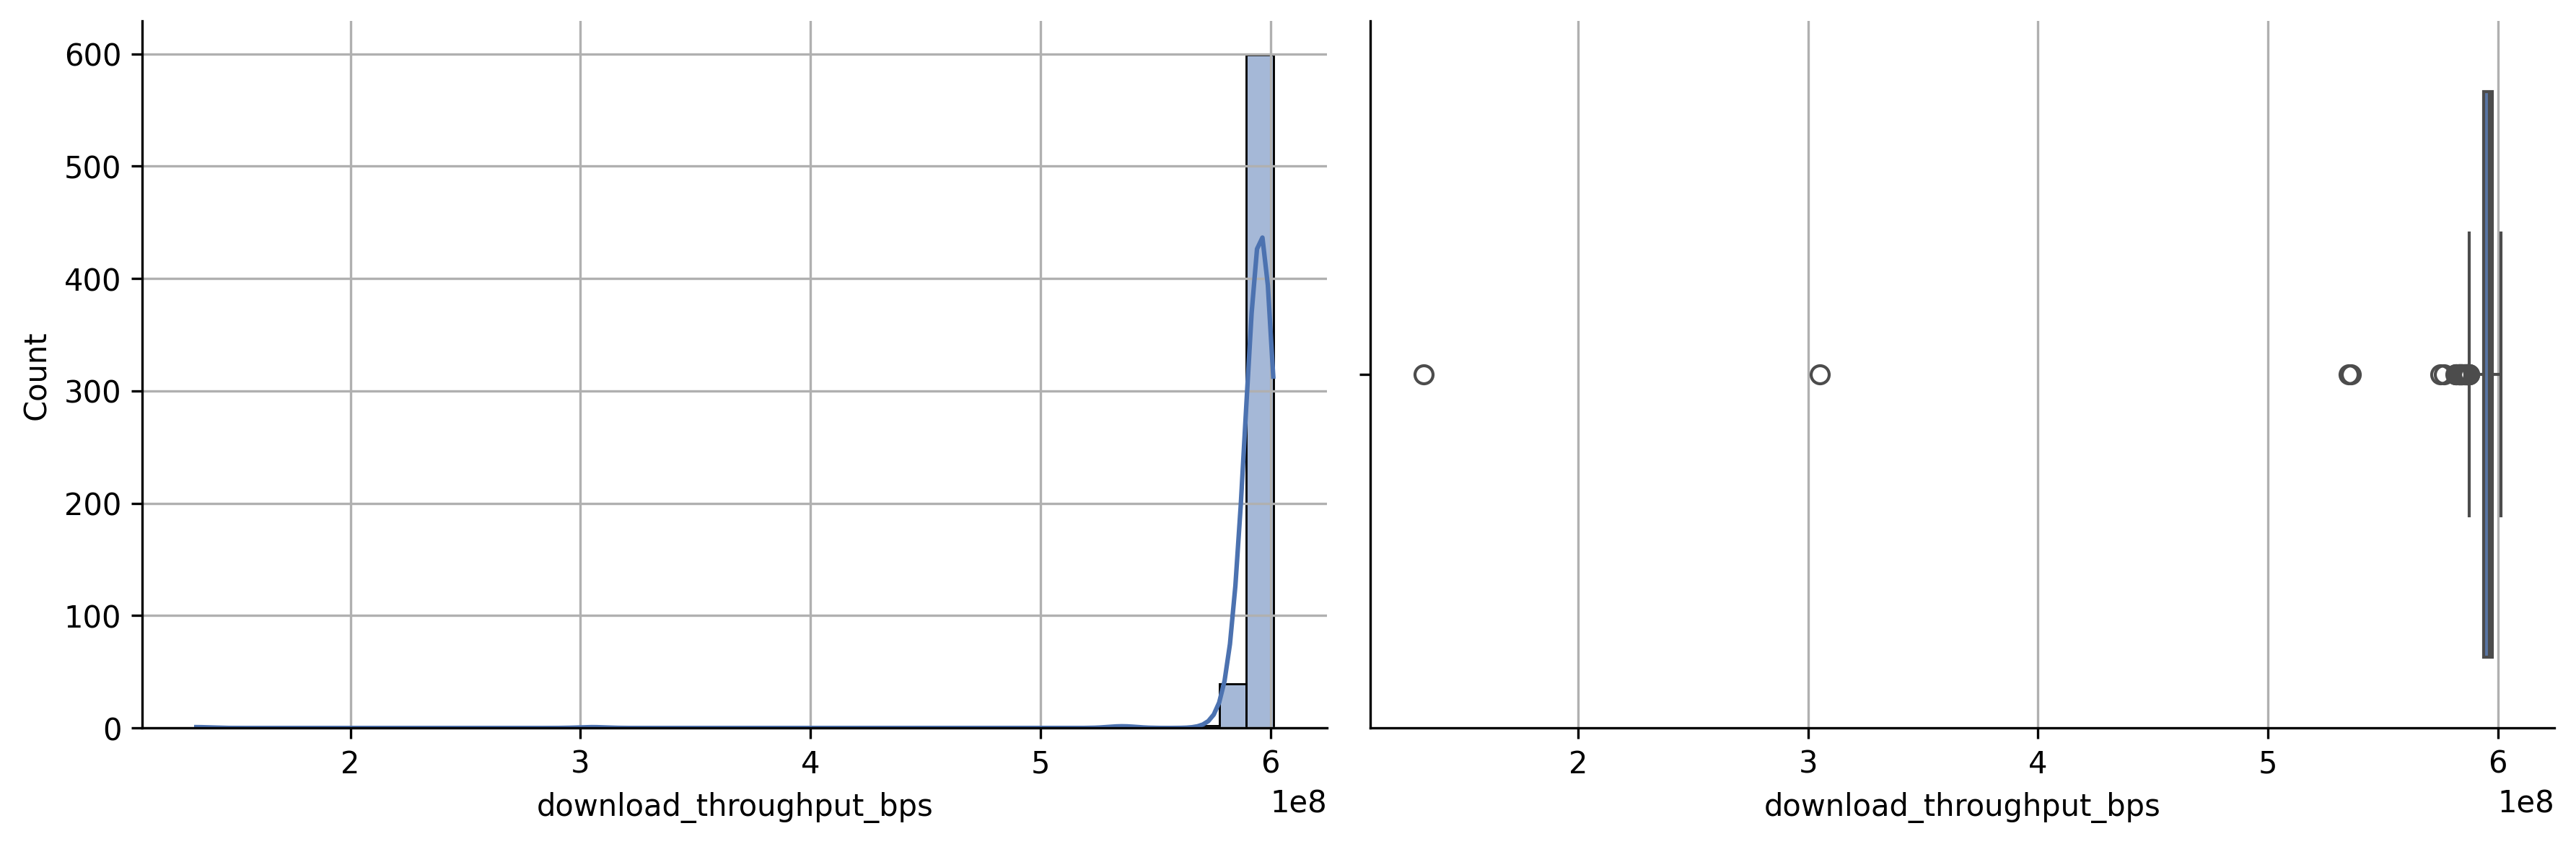
\includegraphics[width=\textwidth]{../figures/eda/chart_download_throughput_bps_client13.png}
	\caption{Taxa média de download (bits/s) para o Cliente 13.}
	\label{fig:chart_download_throughput_bps_client13}
\end{figure}

\begin{figure}[htp]
	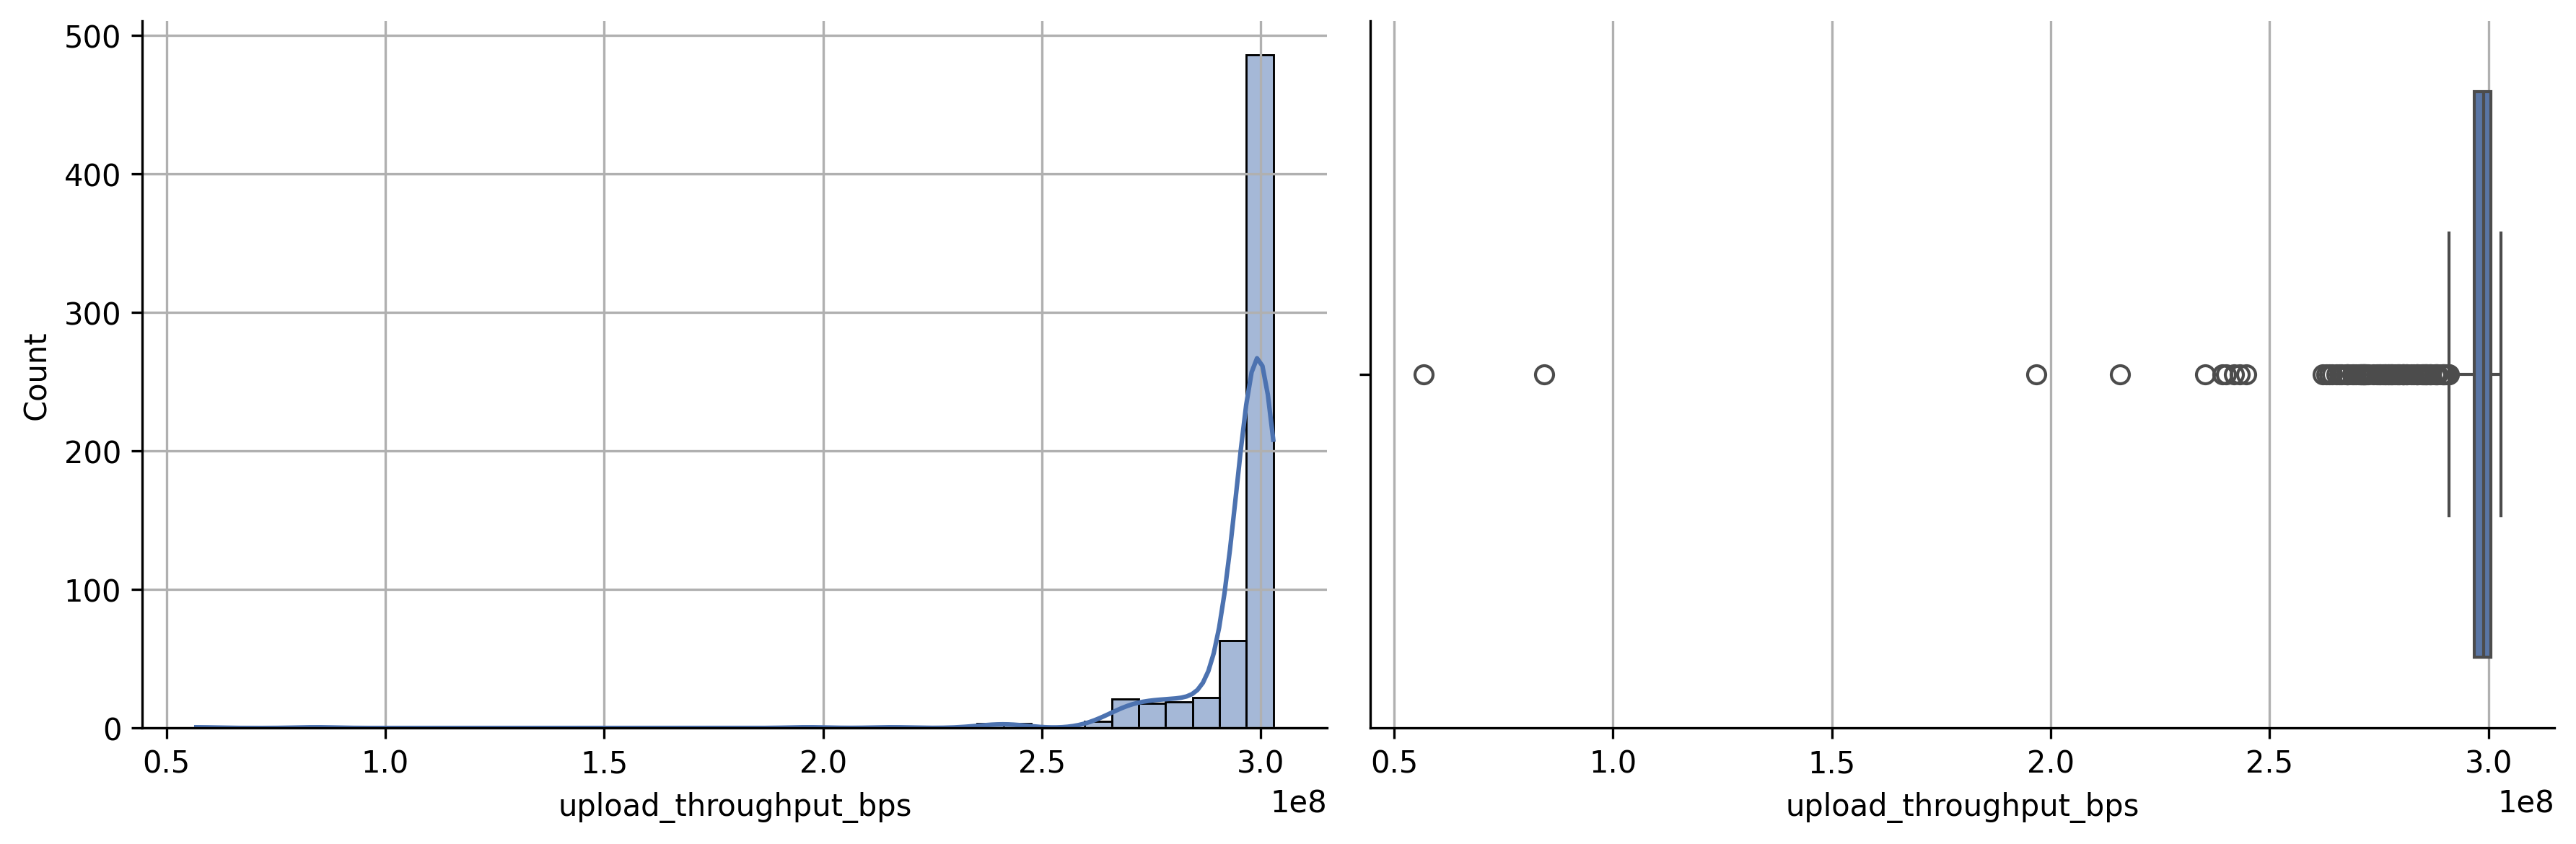
\includegraphics[width=\textwidth]{../figures/eda/chart_upload_throughput_bps_client13.png}
	\caption{Taxa média de upload (bits/s) para o Cliente 13.}
	\label{fig:chart_rtt_download_sec_client13}
\end{figure}

Ao analisar o tempo médio de ida e volta (RTT) para download e upload, ilustrados nas Figuras~\ref{fig:chart_rtt_download_sec_client13} e \ref{fig:chart_rtt_upload_sec_client13}, observa-se um comportamento oposto: há uma concentração de dados à esquerda com uma cauda à direita, indicando que, em geral, o cliente mantém baixa latência, mas com eventos ocasionais de aumento significativo.  
Esses picos de RTT, visíveis como outliers no boxplot, podem estar associados a momentos de sobrecarga momentânea na rede local ou em trechos intermediários da rota de comunicação.

\begin{figure}[htp]
	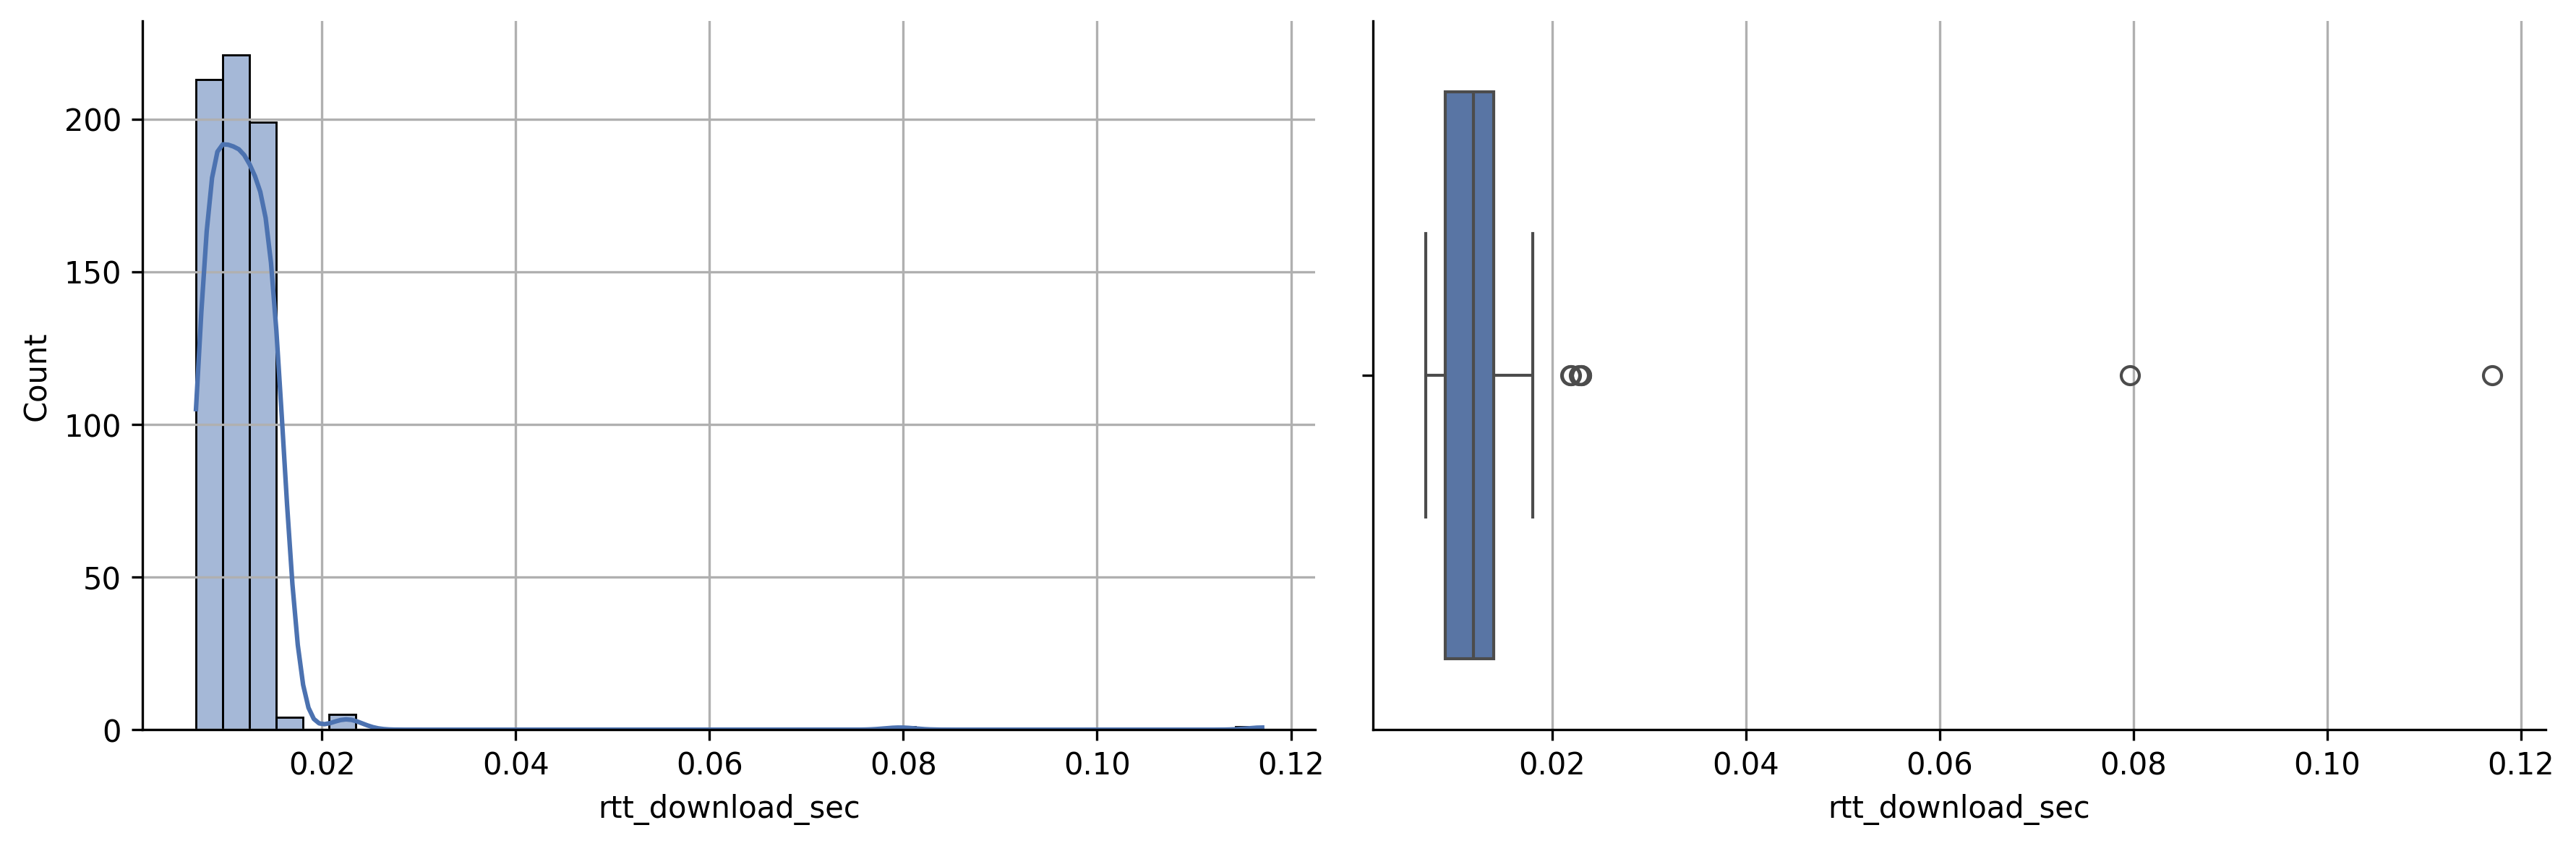
\includegraphics[width=\textwidth]{../figures/eda/chart_rtt_download_sec_client13.png}
	\caption{Tempo médio de ida e volta no download (RTT) (s) para o Cliente 13.}
	\label{fig:chart_upload_throughput_bps_client13}
\end{figure}

\begin{figure}[htp]
	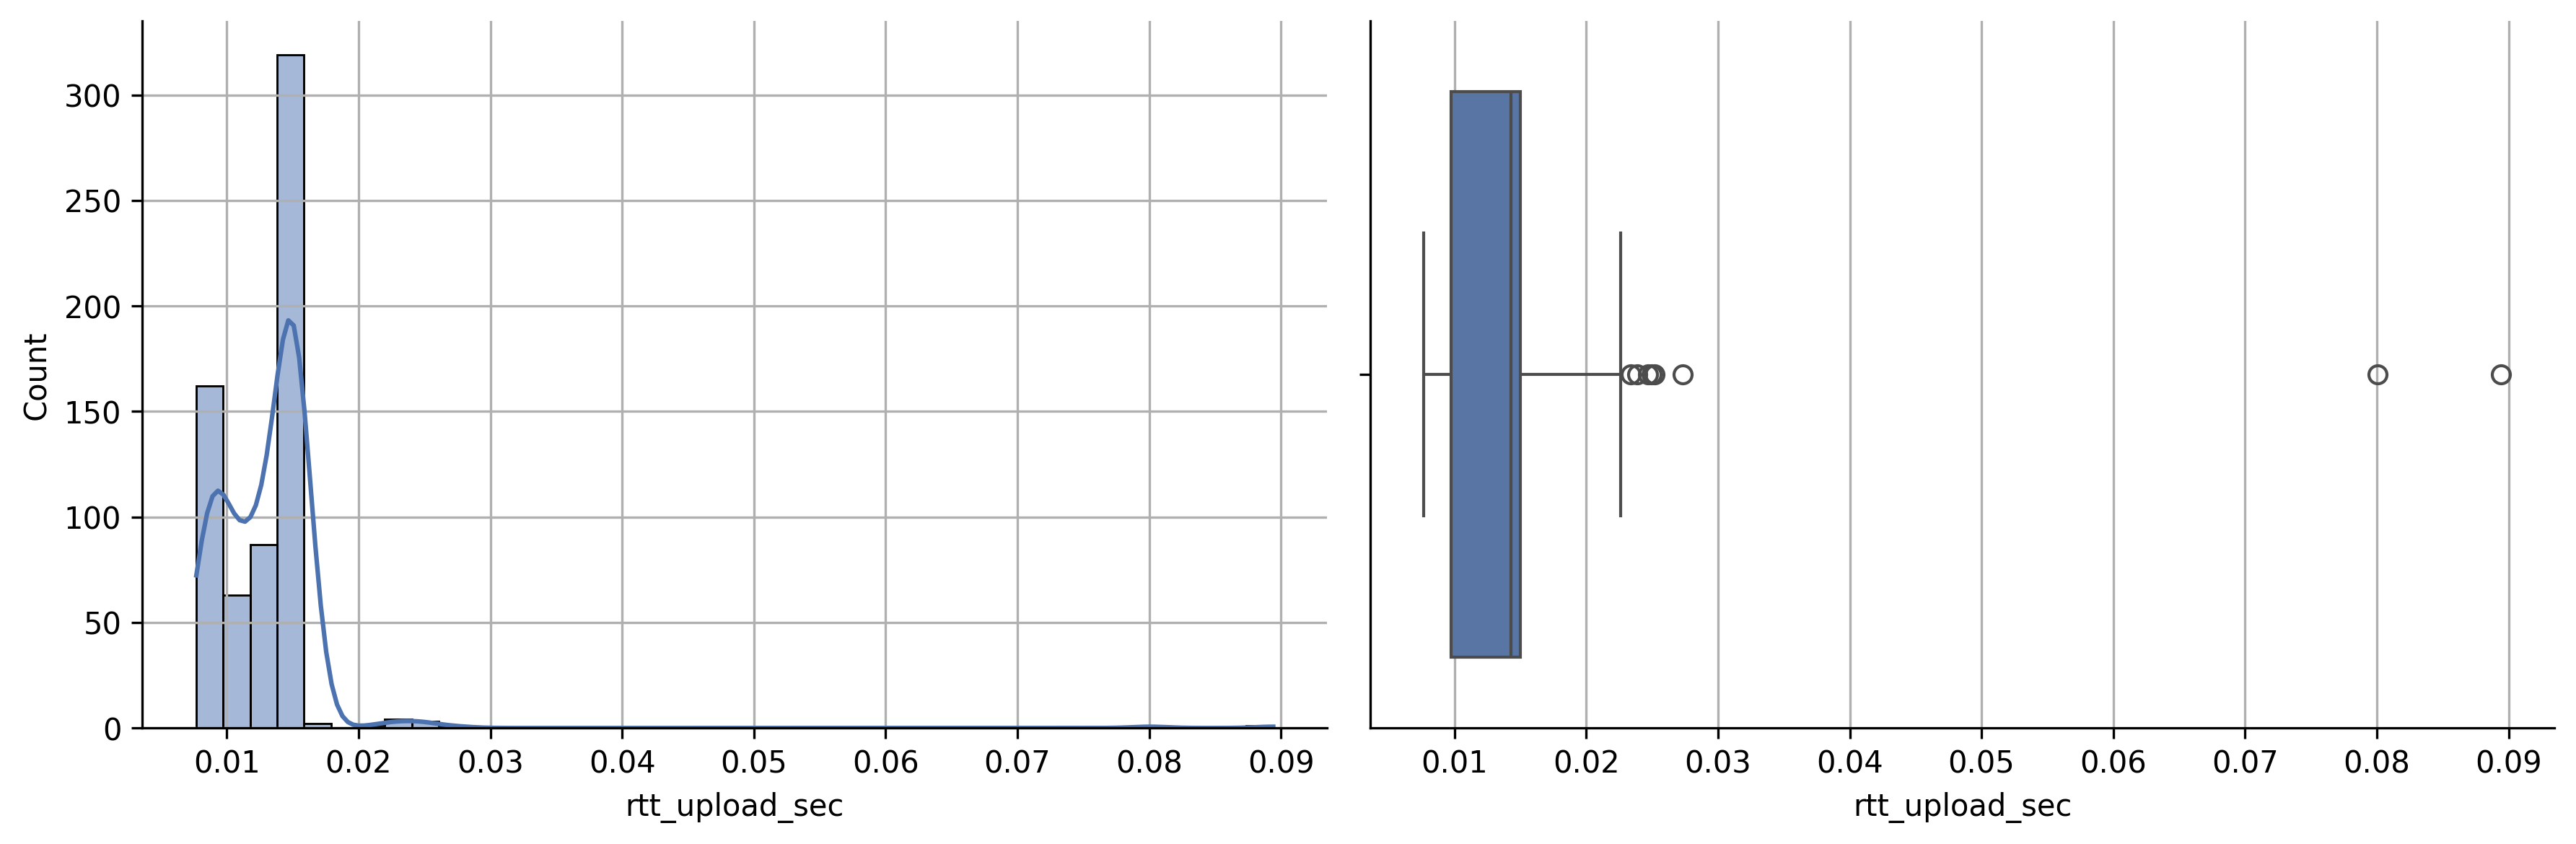
\includegraphics[width=\textwidth]{../figures/eda/chart_rtt_upload_sec_client13.png}
	\caption{Tempo médio de ida e volta no upload (RTT) (s) para o Cliente 13.}
	\label{fig:chart_rtt_upload_sec_client13}
\end{figure}

Por fim, a fração de perda de pacotes (\texttt{packet\_loss\_percent}), apresentada na Figura~\ref{fig:chart_packet_loss_percent_client13}, exibe uma distribuição próxima da normal, com leve tendência bimodal.  
O boxplot mostra poucos outliers à esquerda, indicando uma variação controlada, mas persistente. Esse padrão reforça a hipótese de que o cliente enfrenta um nível crônico de perda de pacotes, refletindo um gargalo mais local do que estrutural.

\begin{figure}[htp]
	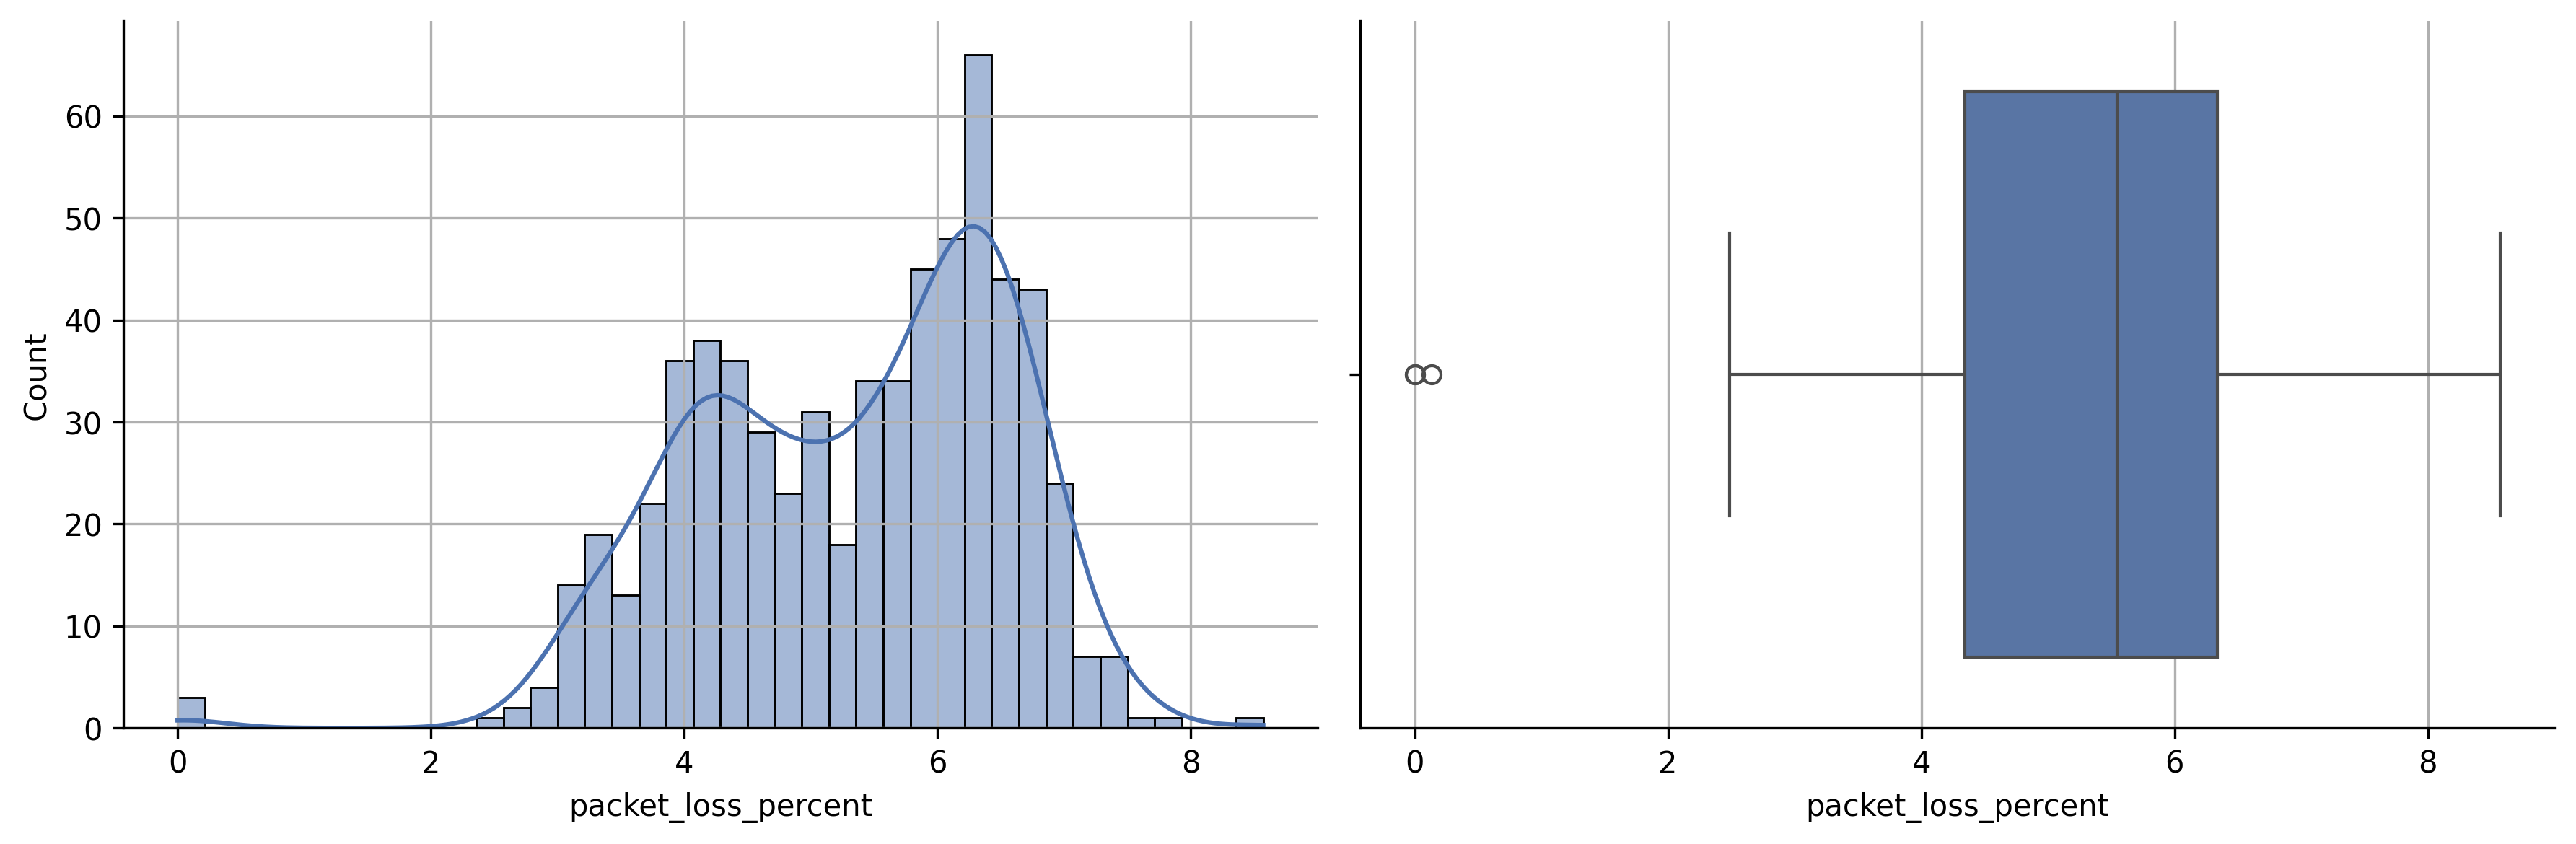
\includegraphics[width=\textwidth]{../figures/eda/chart_packet_loss_percent_client13.png}
	\caption{Fração de perda de pacotes (\%) para o Cliente 13.}
	\label{fig:chart_packet_loss_percent_client13}
\end{figure}

TEXTO AQUI!

\begin{figure}[htp]
	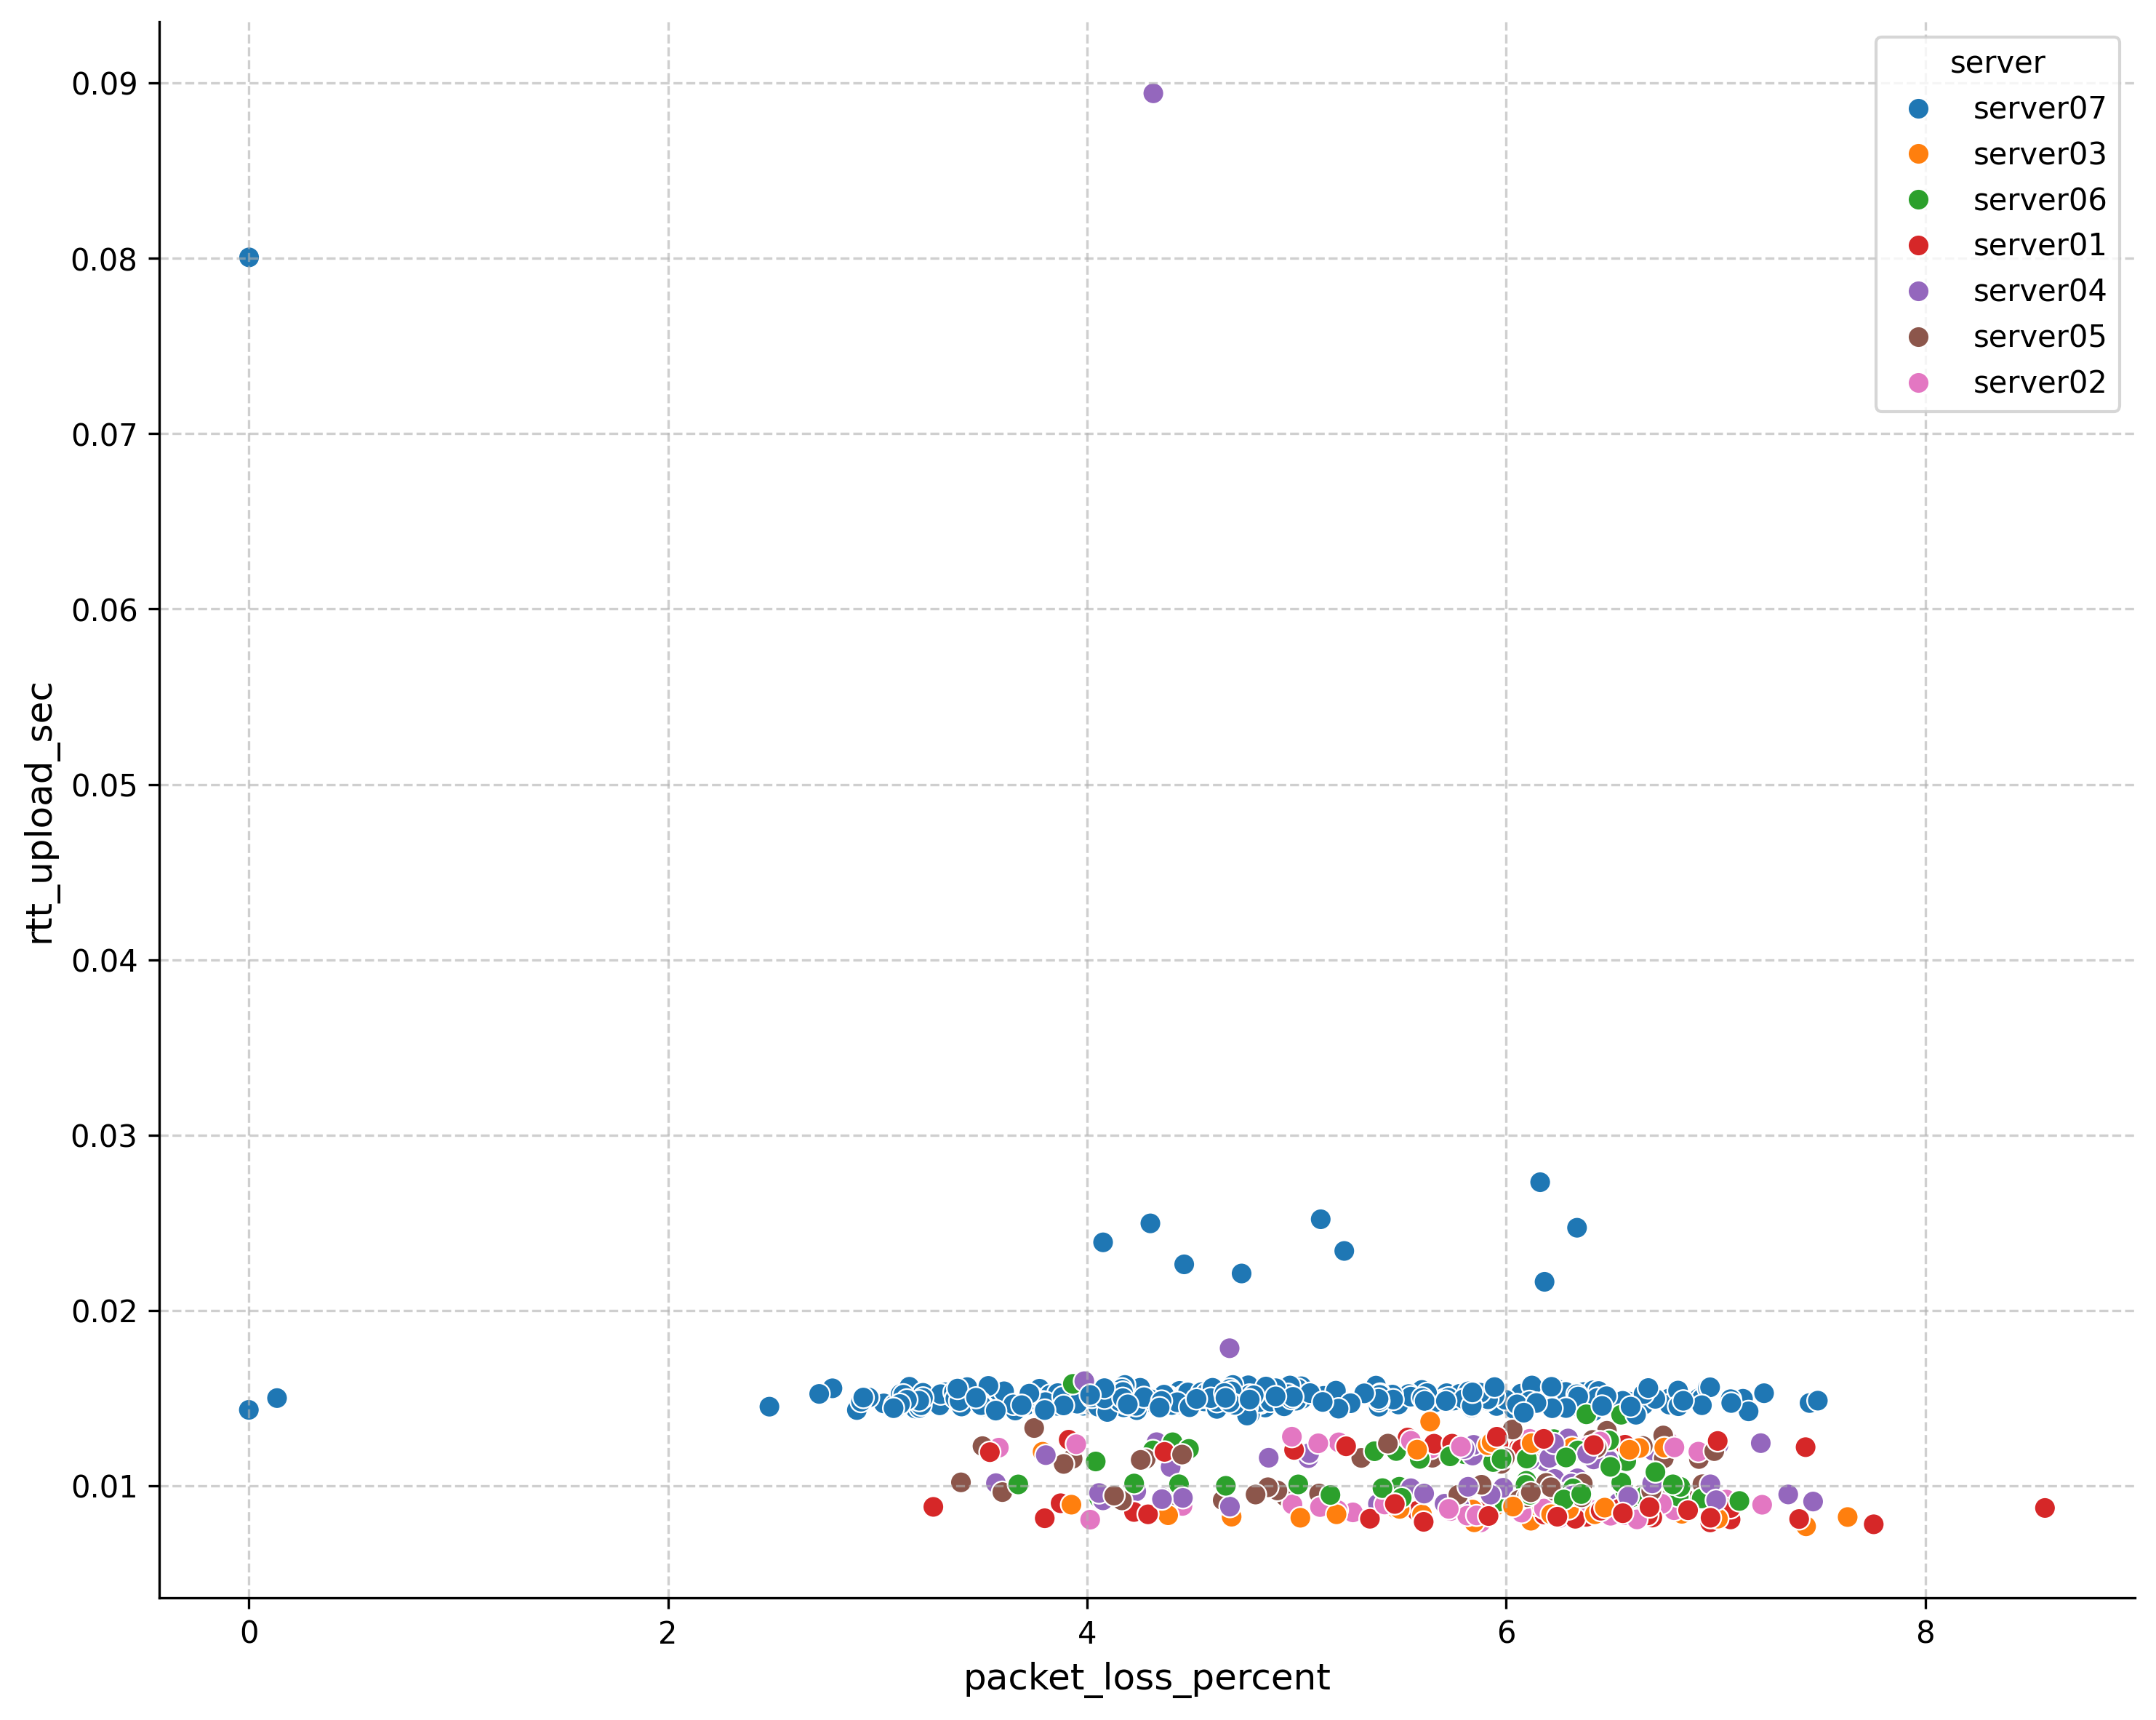
\includegraphics[width=\textwidth]{../figures/eda/scatter_client13.png}
	\caption{MUDAR}
	\label{fig:scatter_client13}
\end{figure}

\subsubsection{Servidor 02}

Para o Servidor 02, as Figuras~\ref{fig:chart_download_throughput_bps_server02} e \ref{fig:chart_upload_throughput_bps_server02} ilustram as taxas médias de download e upload.  
Ambas exibem comportamento aproximadamente uniforme, com leve concentração nos extremos, mais evidente no cenário de download.  
Devido à ampla dispersão dos dados, os boxplots resultam visualmente equilibrados e sem indícios significativos de outliers, sugerindo medições consistentes em uma faixa operacional ampla, característica esperada para um servidor de alta capacidade.

\begin{figure}[htp]
	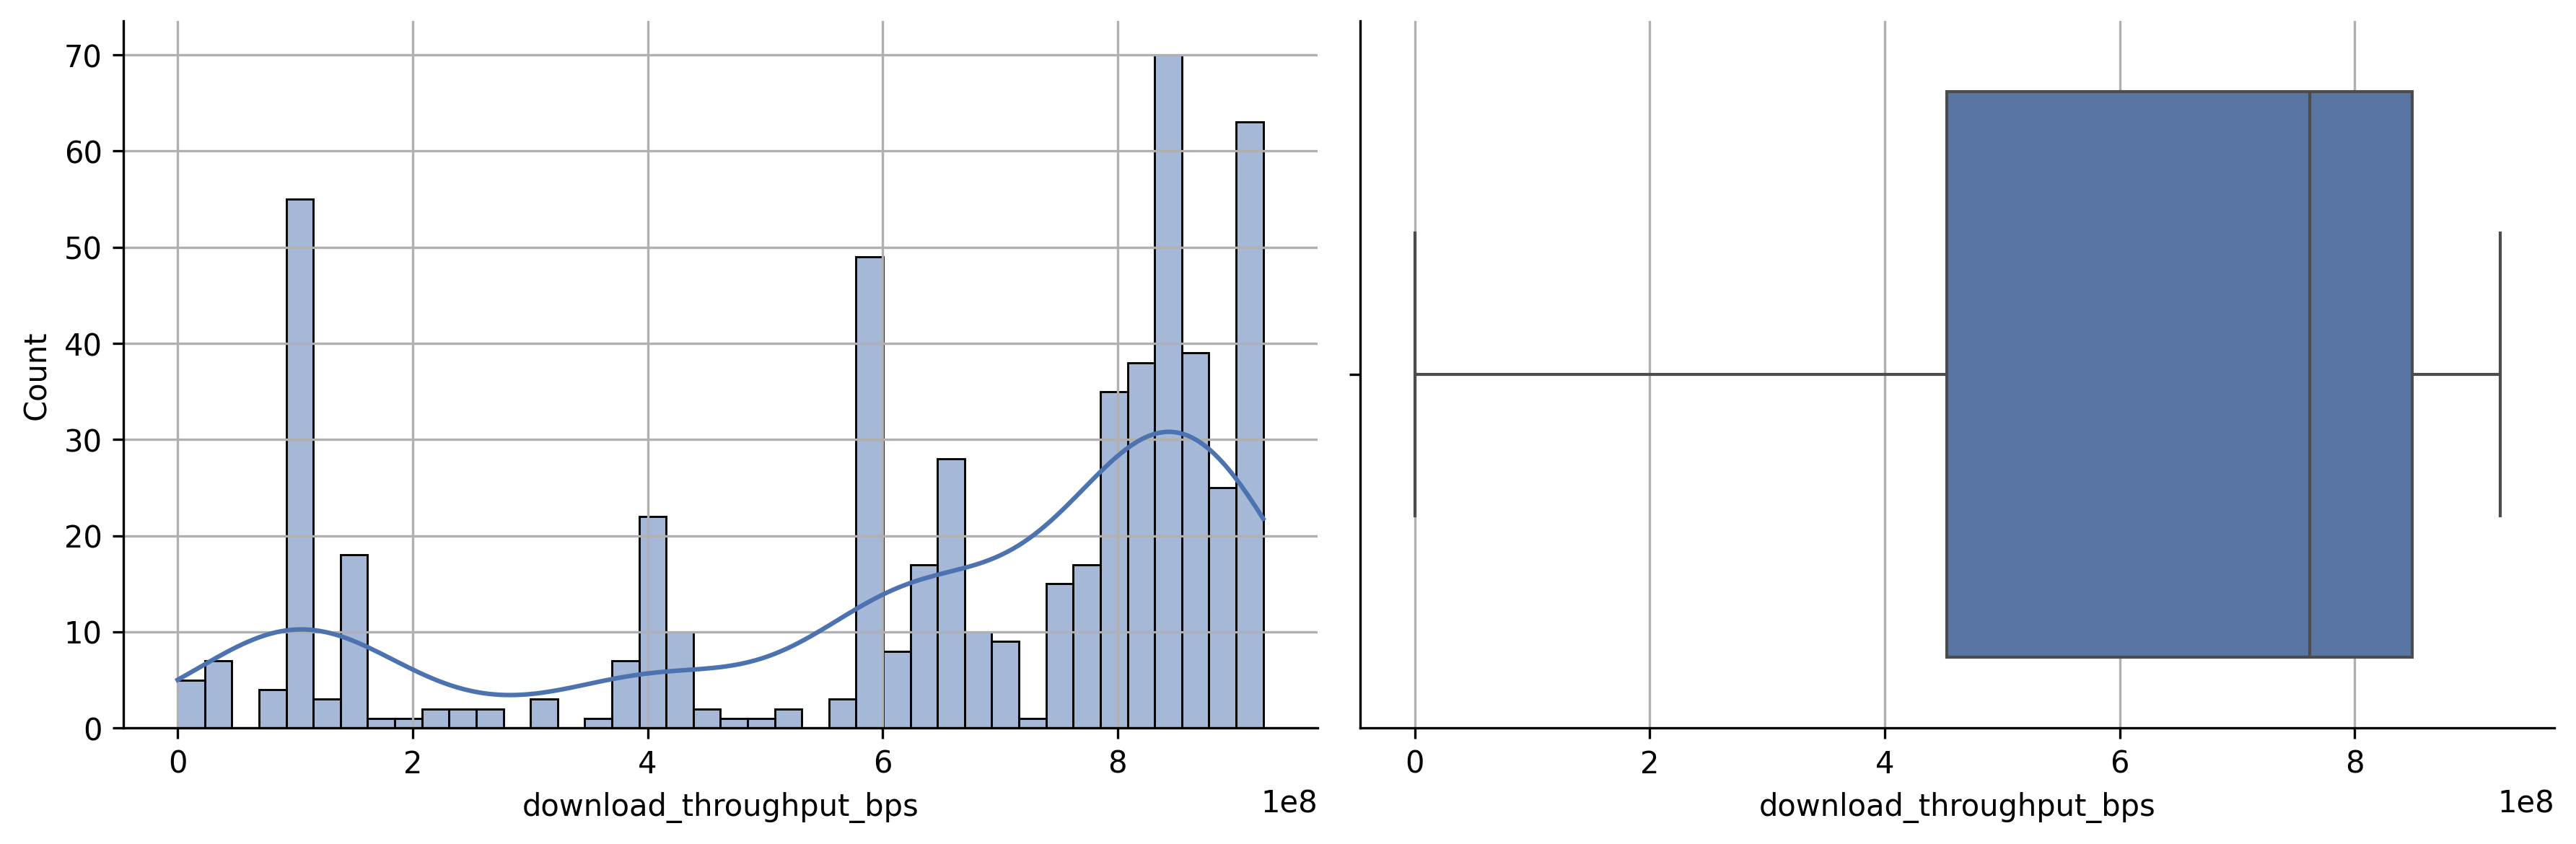
\includegraphics[width=\textwidth]{../figures/eda/chart_download_throughput_bps_server02.png}
	\caption{Taxa média de download (bits/s) para o Servidor 2.}
	\label{fig:chart_download_throughput_bps_server02}
\end{figure}

\begin{figure}[htp]
	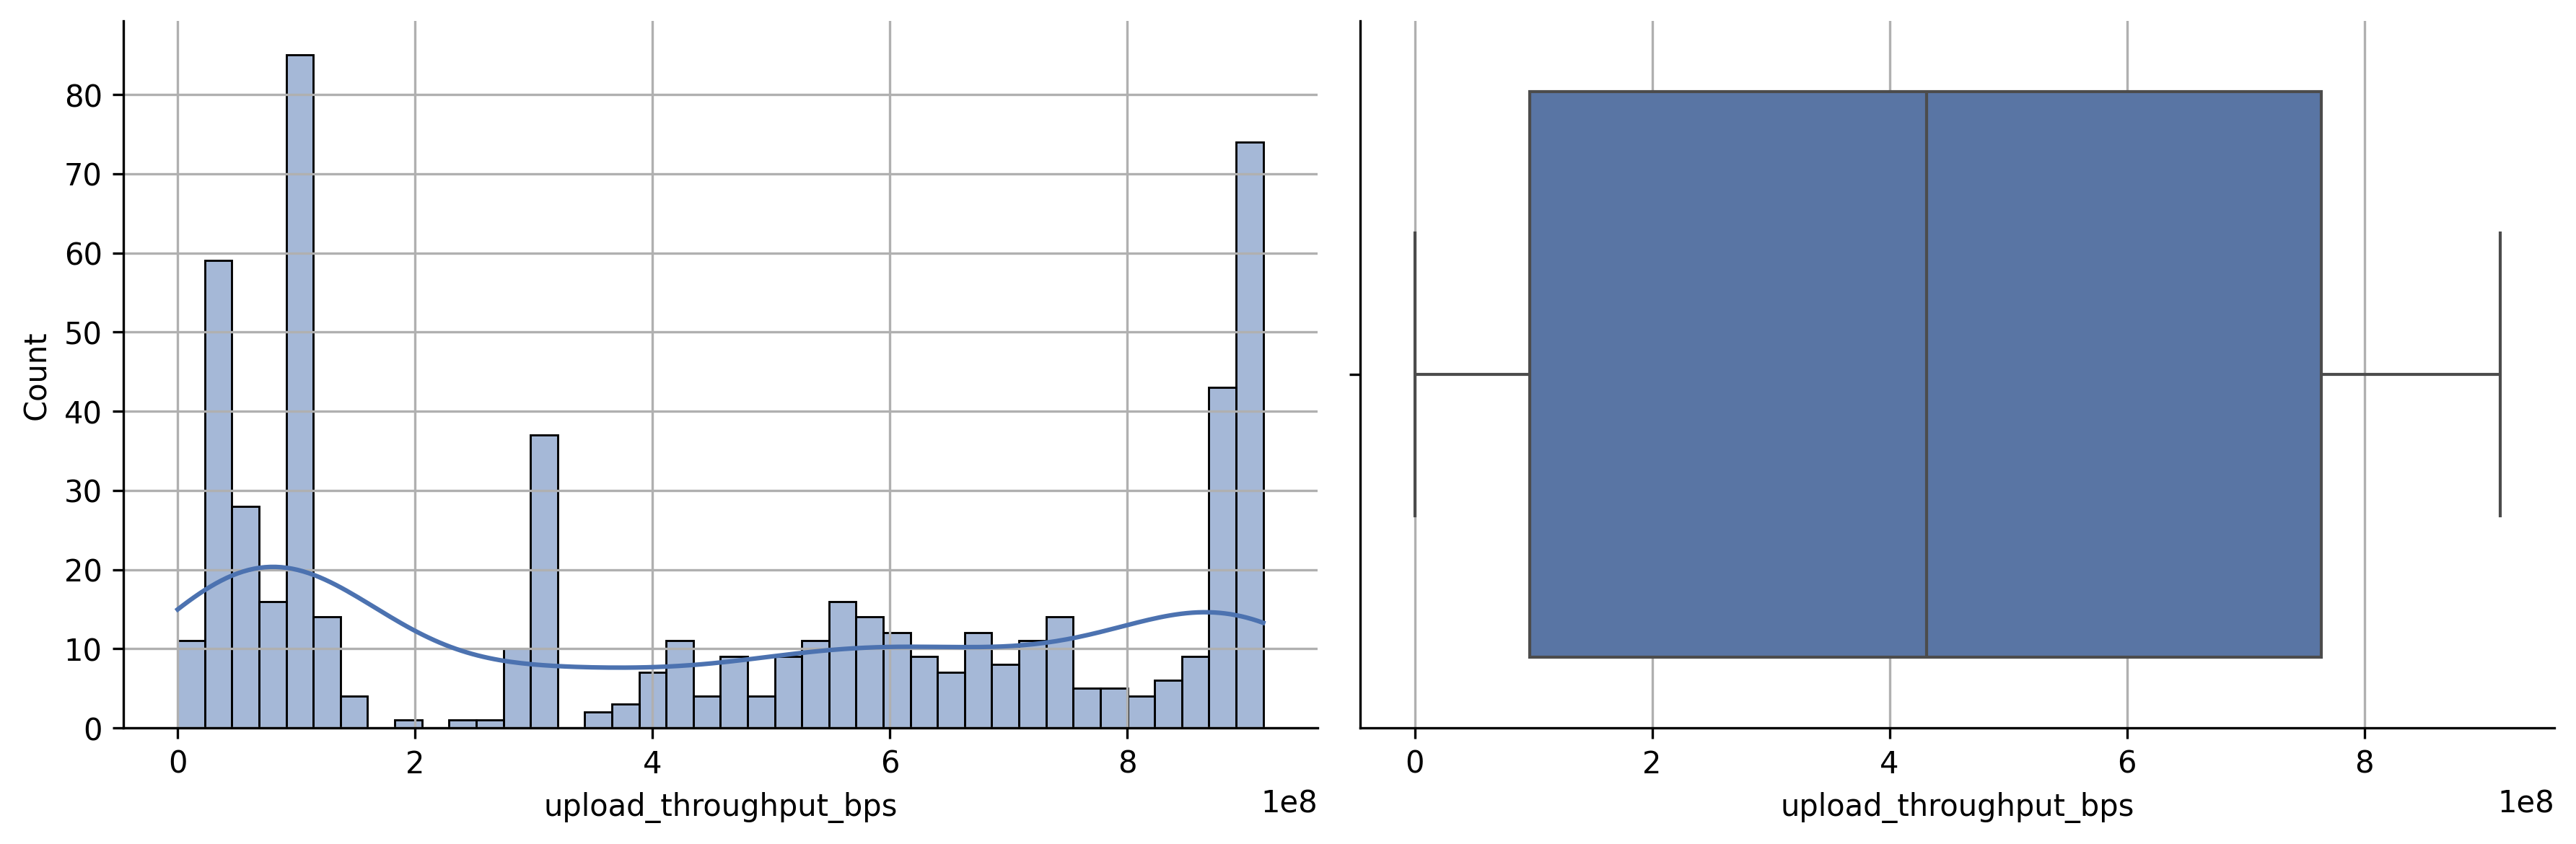
\includegraphics[width=\textwidth]{../figures/eda/chart_upload_throughput_bps_server02.png}
	\caption{Taxa média de upload (bits/s) para o Servidor 2.}
	\label{fig:chart_upload_throughput_bps_server02}
\end{figure}

Os tempos médios de ida e volta (\textit{RTT}) de download e upload, mostrados nas Figuras~\ref{fig:chart_rtt_download_sec_server02} e \ref{fig:chart_rtt_upload_sec_server02}, apresentam comportamentos distintos.  
O RTT de download tende a seguir uma distribuição aproximadamente normal, com uma pequena cauda à direita, o que explica a presença de outliers isolados no boxplot.  
Já o RTT de upload é altamente concentrado à direita, com baixa variabilidade central, uma característica típica de redes otimizadas, mas que também pode gerar a detecção de outliers devido à densidade local elevada.

\begin{figure}[htp]
	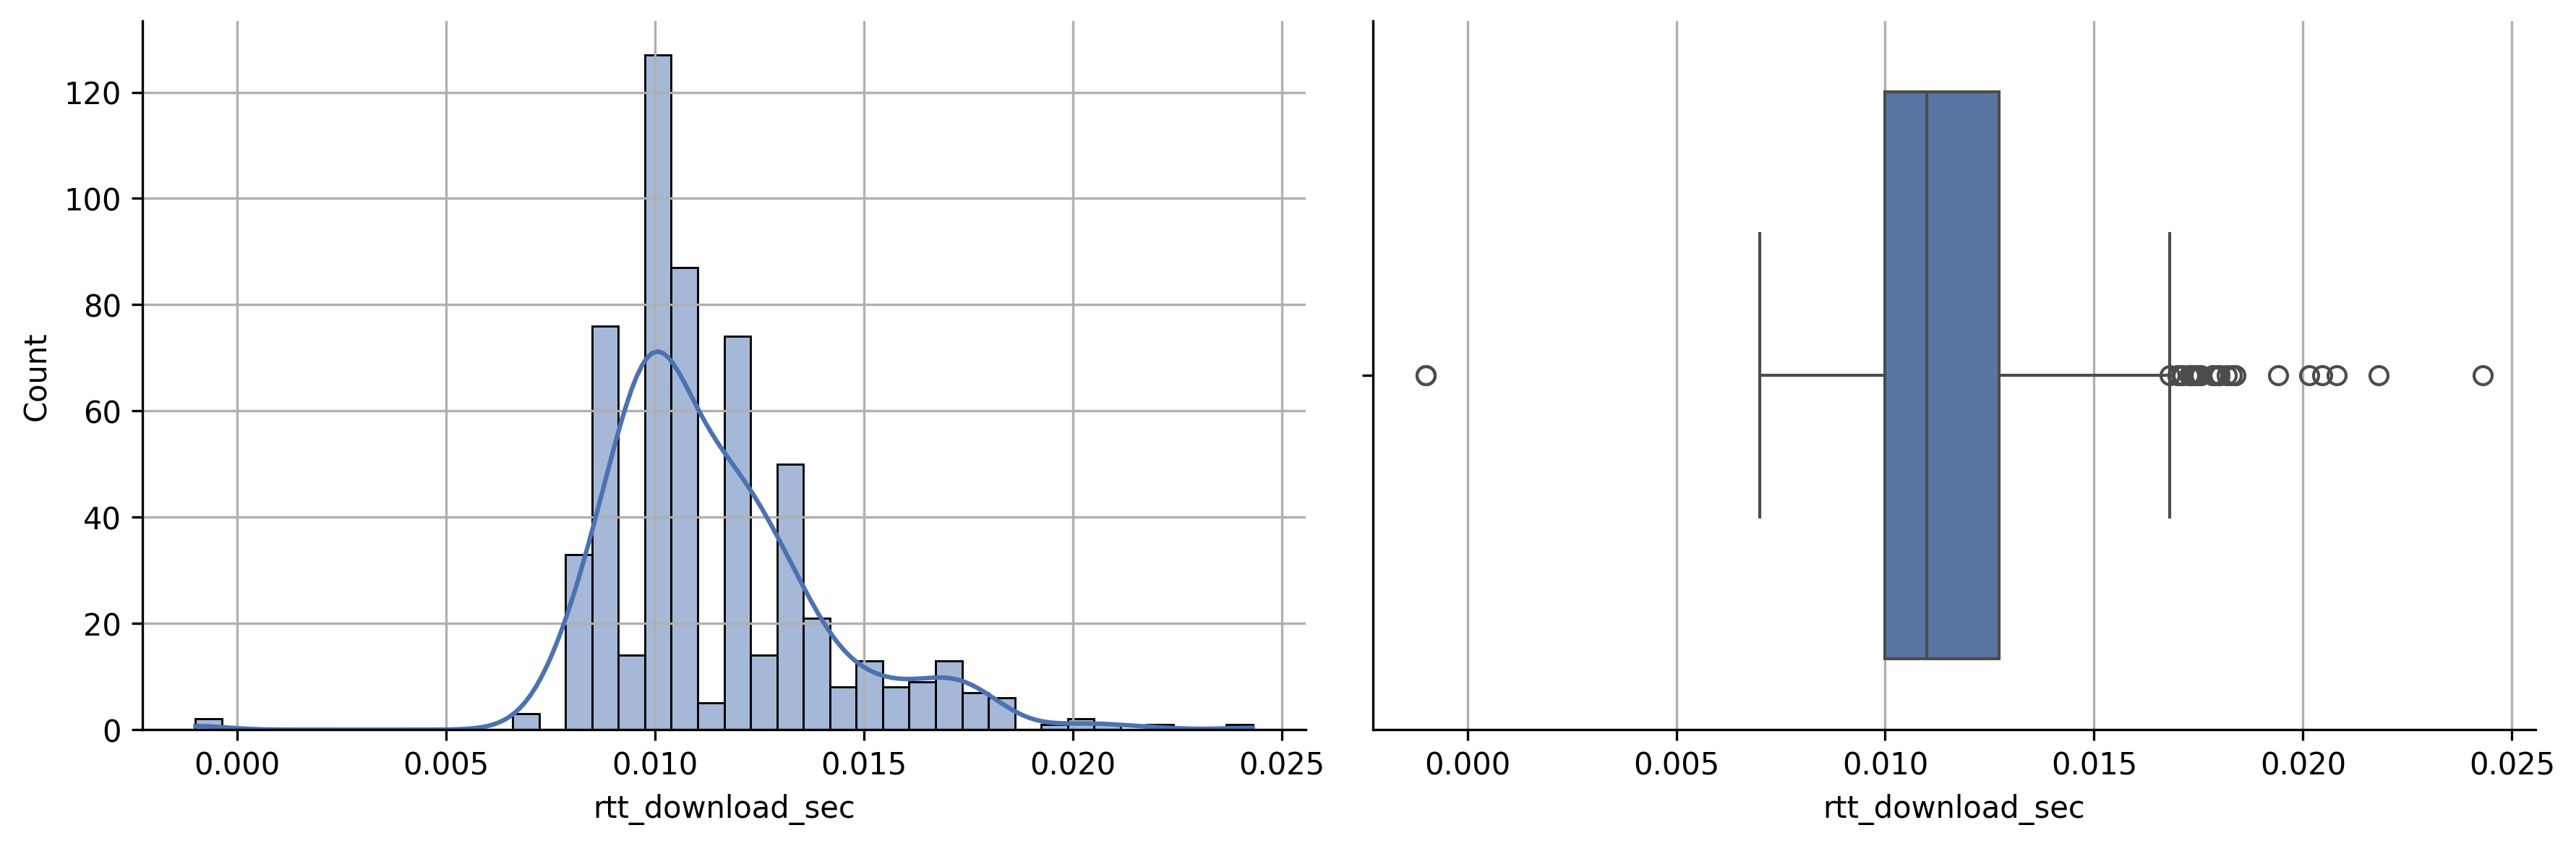
\includegraphics[width=\textwidth]{../figures/eda/chart_rtt_download_sec_server02.png}
	\caption{Tempo médio de ida e volta no download (RTT) (s) para o Servidor 2.}
	\label{fig:chart_rtt_download_sec_server02}
\end{figure}

\begin{figure}[htp]
	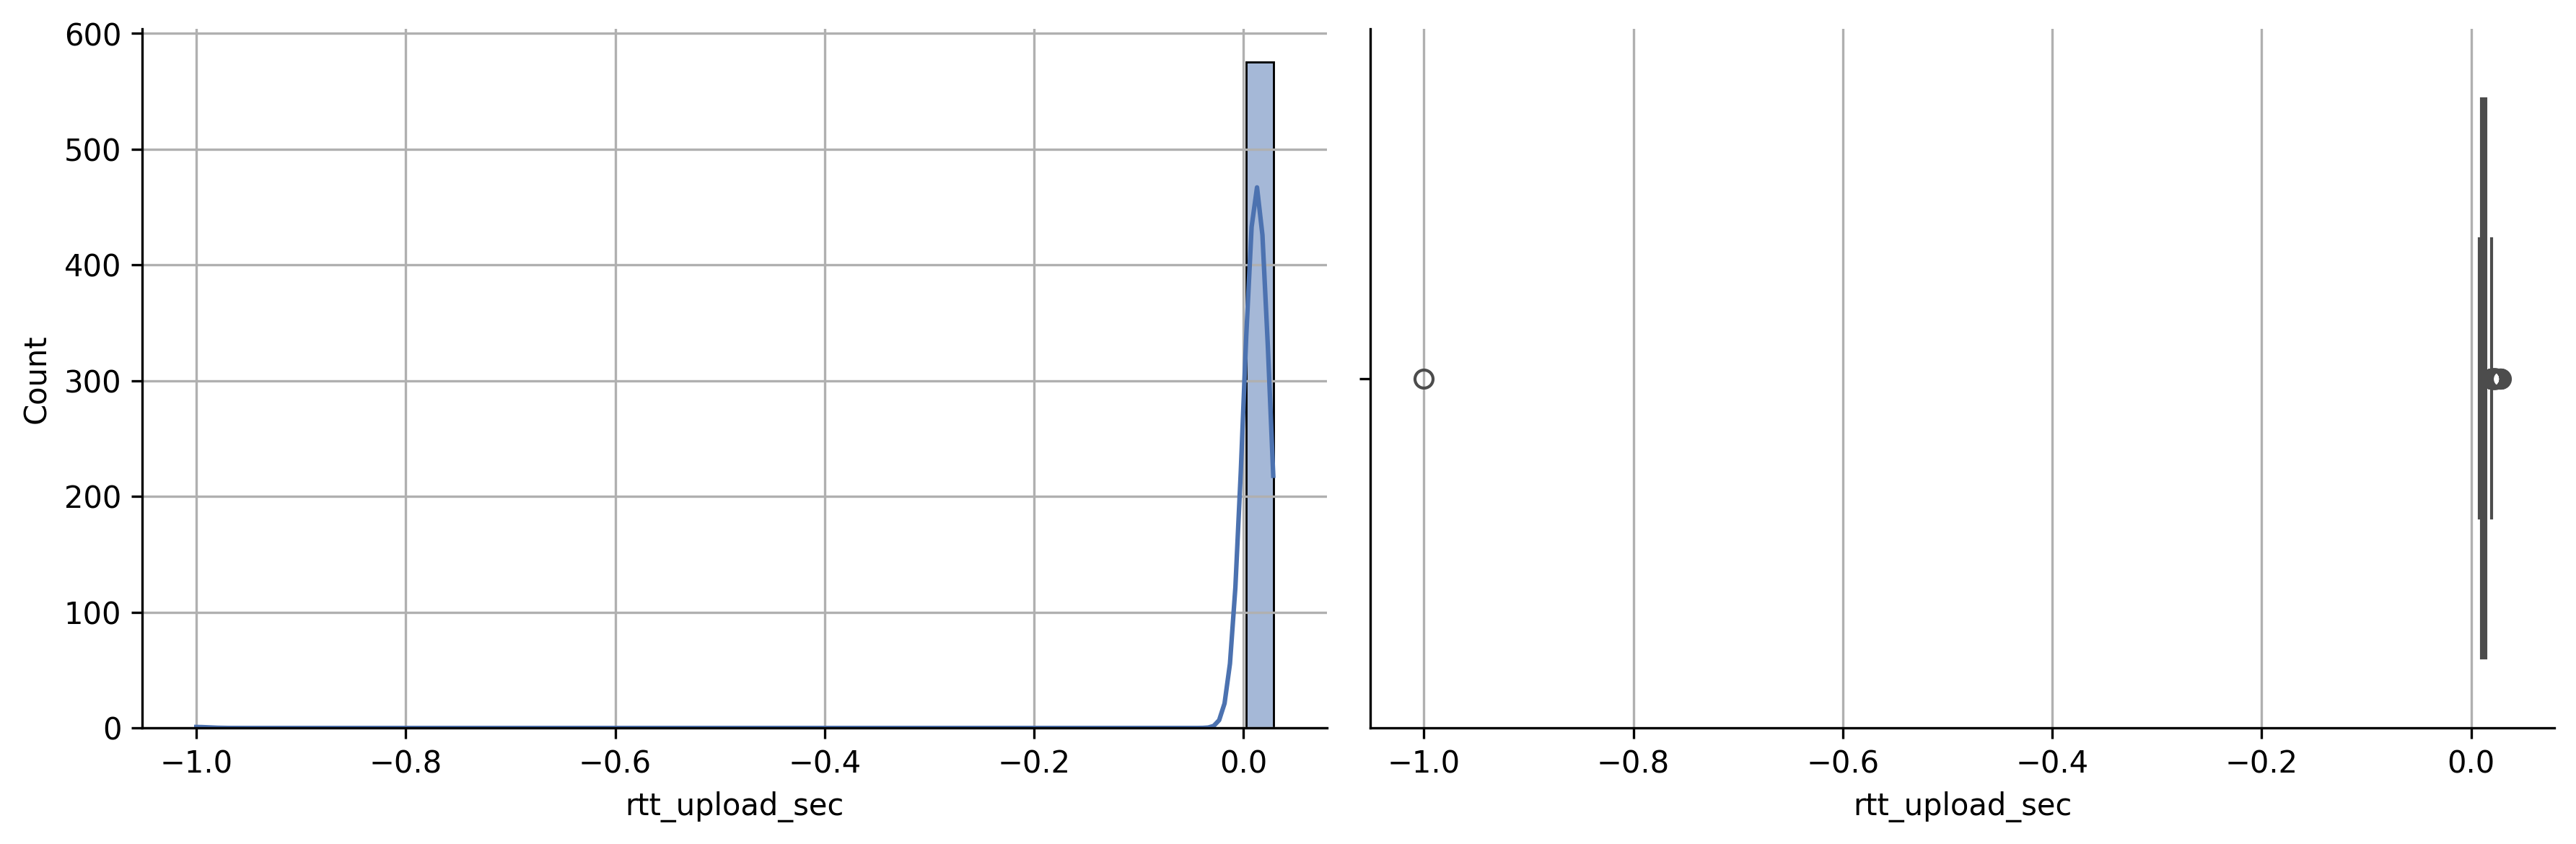
\includegraphics[width=\textwidth]{../figures/eda/chart_rtt_upload_sec_server02.png}
	\caption{Tempo médio de ida e volta no upload (RTT) (s) para o Servidor 2.}
	\label{fig:chart_rtt_upload_sec_server02}
\end{figure}

Por fim, a fração de perda de pacotes (Figura \ref{fig:chart_packet_loss_percent_server02}) mostra forte concentração à esquerda e uma cauda à direita mais extensa.  
Embora o boxplot indique vários outliers, isso decorre principalmente da alta densidade de valores próximos a zero, o que aumenta a sensibilidade dos limites interquartis.

\begin{figure}[htp]
	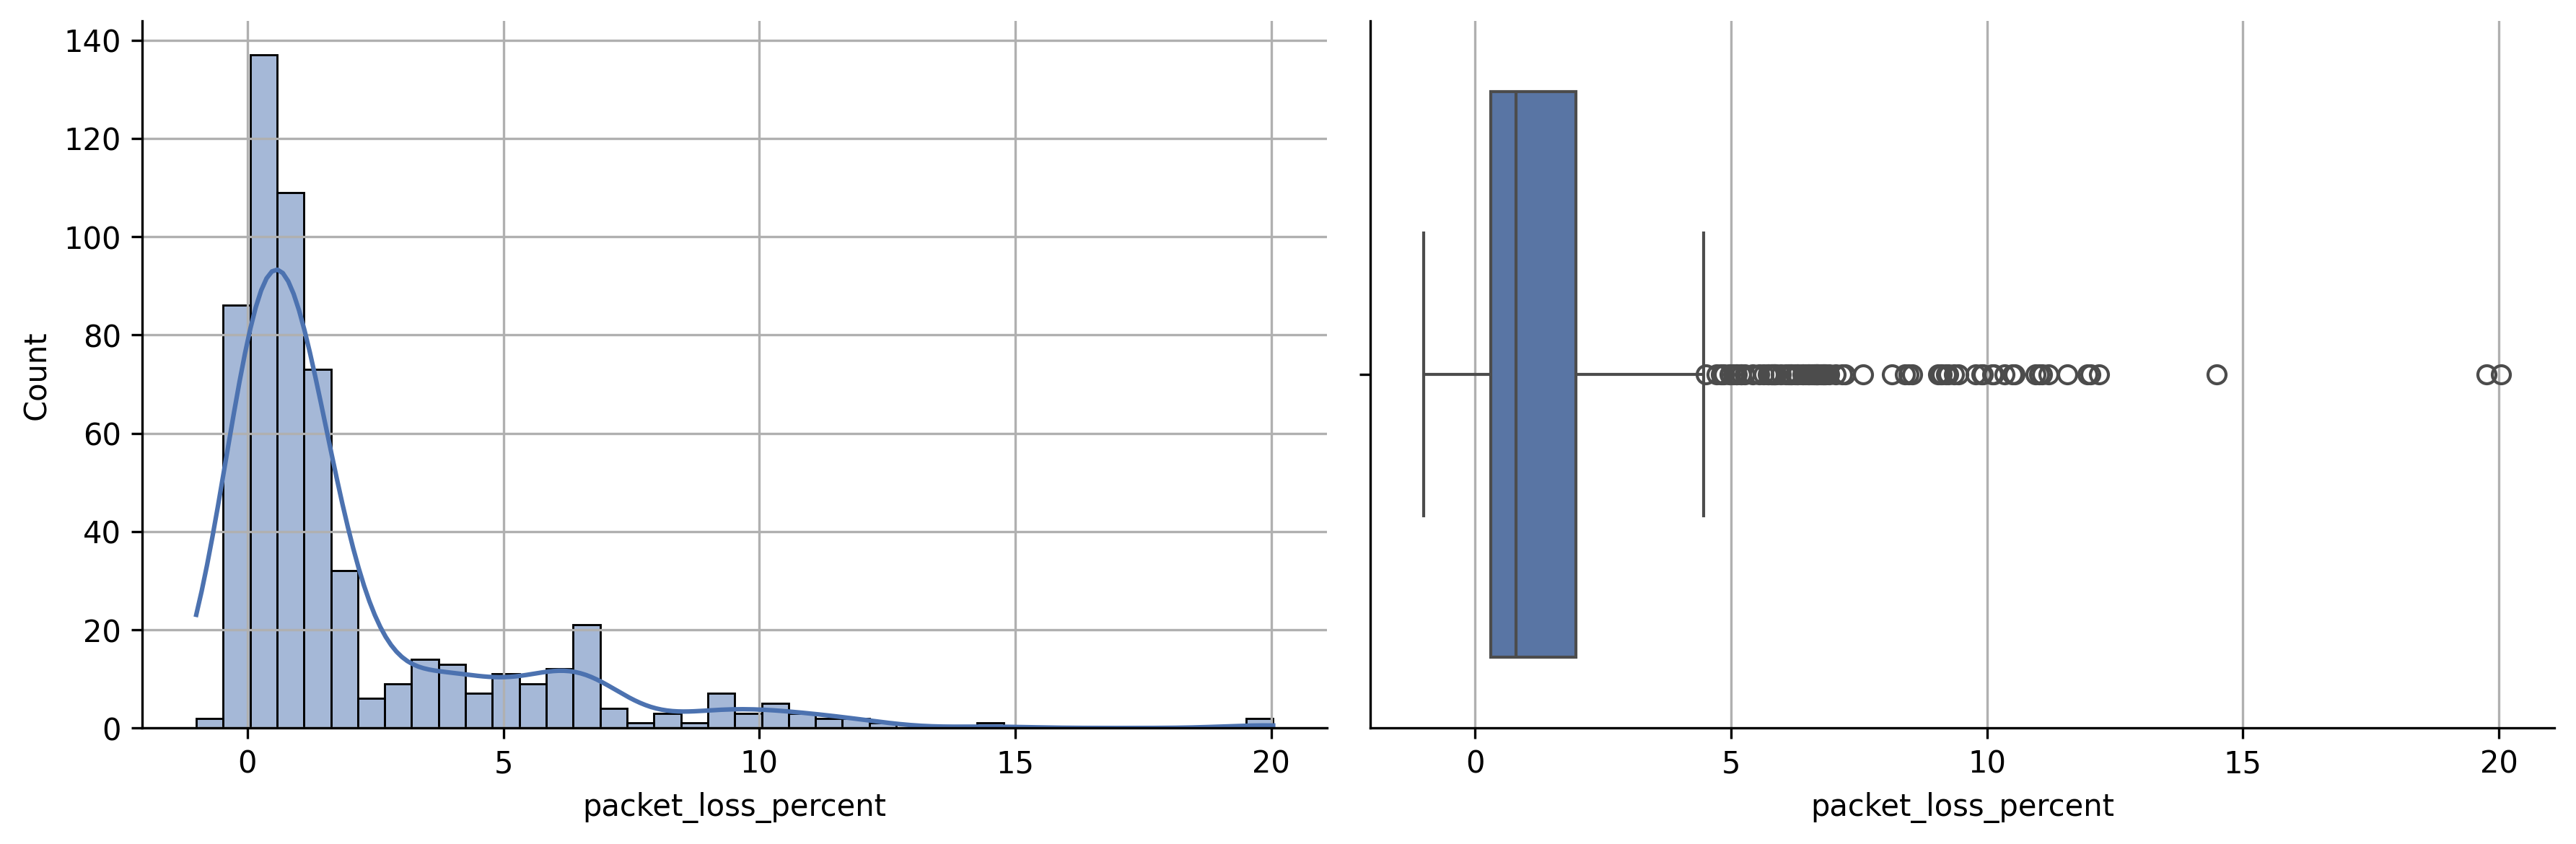
\includegraphics[width=\textwidth]{../figures/eda/chart_packet_loss_percent_server02.png}
	\caption{Fração de perda de pacotes (\%) para o Servidor 2.}
	\label{fig:chart_packet_loss_percent_server02}
\end{figure}

TEXTO AQUI!

\begin{figure}[htp]
	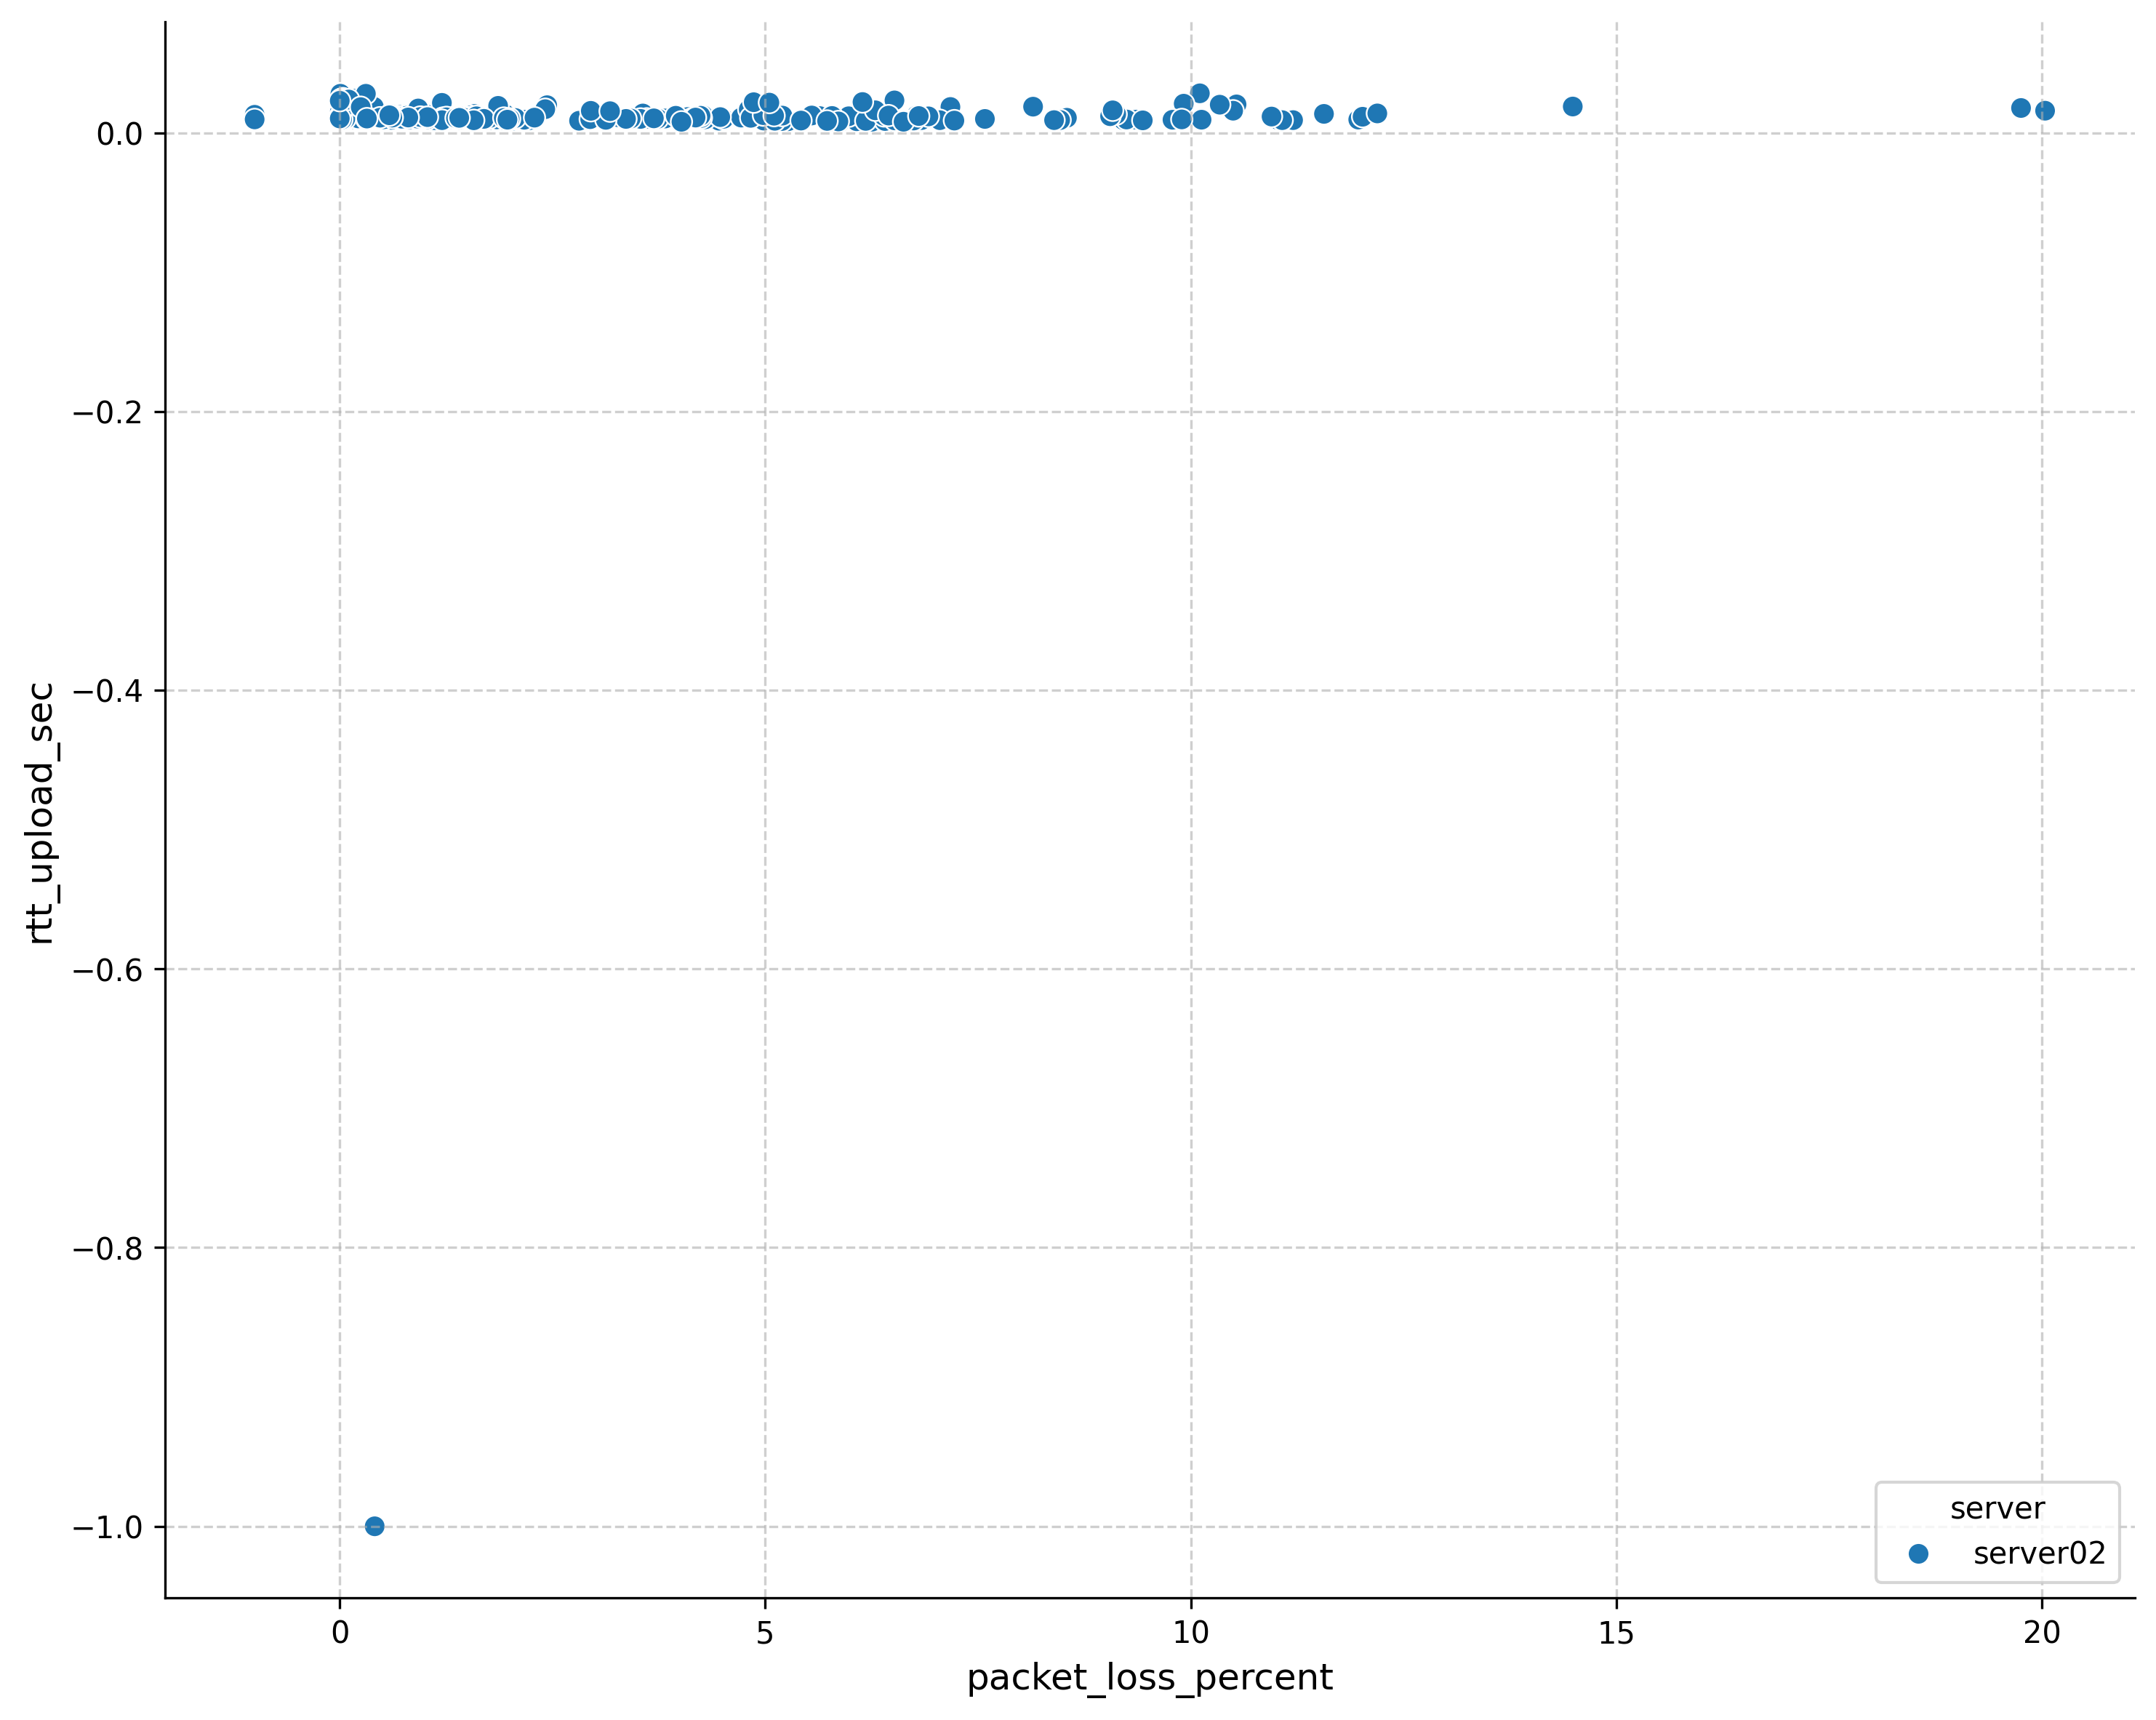
\includegraphics[width=\textwidth]{../figures/eda/scatter_server02.png}
	\caption{MUDAR}
	\label{fig:scatter_server02}
\end{figure}

\subsubsection{Síntese e Próximos Passos}
Os resultados apresentados indicam diferenças significativas entre o comportamento das métricas de desempenho do Cliente 13 e do Servidor 02.  
Enquanto o primeiro exibe padrões mais concentrados e indícios de saturação ou gargalo local, o segundo apresenta variabilidade mais ampla e características consistentes com um ambiente de rede estável e de alta capacidade.  

Essas observações servirão de base para a próxima etapa do estudo, onde serão definidas as distribuições probabilísticas mais adequadas a cada variável, com base tanto nas sugestões do trabalho quanto nas evidências empíricas observadas, que serão posteriormente utilizadas na modelagem por \textbf{Máxima Verossimilhança (MLE)} e \textbf{Inferência Bayesiana}.  
Antes disso, entretanto, apresenta-se uma breve discussão teórica sobre as distribuições candidatas e suas propriedades.

\subsection{Distribuições de Probabilidade e Pares Conjugados}

As distribuições de probabilidade diferem em seus domínios e nas variáveis que modelam. Na inferência Bayesiana, certos pares de distribuições, conhecidos como pares conjugados, são cruciais, pois a distribuição posterior (após a observação dos dados) pertence à mesma família da distribuição prior.

\subsubsection{Distribuições Fundamentais}

\begin{enumerate}
	\item \textbf{Distribuição Normal (Gaussiana, $\mathcal{N}$):}
	\begin{itemize}
		\item \textit{Domínio:} $(-\infty, +\infty)$.
		\item \textit{Função:} Modela fenômenos simétricos e erros de medição.
		\item \textit{PDF:} $$f(x|\mu, \sigma^2) = \frac{1}{\sqrt{2\pi\sigma^2}} e^{-\frac{(x-\mu)^2}{2\sigma^2}}$$
	\end{itemize}
	
	\item \textbf{Distribuição Gama ($\Gamma$):}
	\begin{itemize}
		\item \textit{Domínio:} $(0, +\infty)$.
		\item \textit{Função:} Modela tempos de espera/vida ou somas de variáveis exponenciais (não-negativas).
		\item \textit{PDF:} $$f(x|k, \theta) = \frac{x^{k-1}e^{-x/\theta}}{\Gamma(k)\theta^k}$$
	\end{itemize}
	
	\item \textbf{Distribuição Beta ($\mathcal{B}$):}
	\begin{itemize}
		\item \textit{Domínio:} $[0, 1]$.
		\item \textit{Função:} Modela probabilidades, proporções e taxas de sucesso/falha.
		\item \textit{PDF:} $$f(x|\alpha, \beta) = \frac{x^{\alpha-1}(1-x)^{\beta-1}}{B(\alpha, \beta)}$$
	\end{itemize}
\end{enumerate}

\subsubsection{Pares de Distribuições Conjugadas}

O conceito de par conjugado simplifica o cálculo da distribuição posterior na inferência Bayesiana:

\begin{enumerate}
	\item \textbf{Normal-Normal (Prior-Likelihood):}
	\begin{itemize}
		\item \textit{Função:} Usado para inferir a média ($\mu$) de uma distribuição Normal (Likelihood), quando a variância ($\sigma^2$) é conhecida.
		\item \textit{Conjugado:} A distribuição Normal é a prior conjugada para a média de dados amostrados de uma distribuição Normal.
		\item \textit{Propriedade:} Se a prior de $\mu$ é Normal, a posterior de $\mu$ também será Normal.
	\end{itemize}
	
	\item \textbf{Beta-Binomial (Prior-Likelihood):}
	\begin{itemize}
		\item \textit{Função:} Usado para inferir a probabilidade de sucesso ($p$) em experimentos de Bernoulli/Binomial.
		\item \textit{Conjugado:} A distribuição Beta é a prior conjugada para o parâmetro de probabilidade de sucesso ($p$) de dados Binomiais (Likelihood).
		\item \textit{Propriedade:} Se a prior de $p$ é Beta ($\mathcal{B}(\alpha, \beta)$), a posterior de $p$ também será Beta ($\mathcal{B}(\alpha + k, \beta + n - k)$, onde $k$ são os sucessos em $n$ ensaios).
	\end{itemize}
	
	\item \textbf{Gamma-Gamma (Prior-Likelihood):}
	\begin{itemize}
		\item \textit{Função:} Usado para inferir a taxa ($\lambda$) de um processo de Poisson ou para inferir o parâmetro de precisão (inverso da escala) de uma distribuição Normal.
		\item \textit{Conjugado:} A distribuição Gama é a prior conjugada para o parâmetro de taxa ($\lambda$) de dados amostrados de uma distribuição Poisson ou de uma distribuição Exponencial/Gama.
		\item \textit{Propriedade:} Se a prior da taxa é Gama, a posterior da taxa também será Gama.
	\end{itemize}
\end{enumerate}
\footnotesize 
Nota: $\mu$ é a média e $\sigma^2$ é a variância; $k$ (forma) e $\theta$ (escala) são os parâmetros da Gama; $\alpha$ e $\beta$ (parâmetros de forma) são os parâmetros da Beta; $B$ é a função Beta, e $\Gamma$ é a função Gama.
\normalsize

\subsubsection{Modelos Probabilísticos Adotados}

Com base nas análises exploratórias realizadas, foi possível identificar padrões distintos
no comportamento das variáveis medidas, permitindo selecionar modelos paramétricos
adequados a cada caso. A escolha de cada distribuição baseia-se nas propriedades
estatísticas e físicas dos dados, como domínio de definição, forma da distribuição e
presença de assimetrias, garantindo que os modelos adotados sejam coerentes com o
fenômeno observado.

\begin{itemize}
	\item \textbf{Throughput (Download e Upload):}
	apresenta valores exclusivamente positivos e forte assimetria à direita,
	característica típica de medições de taxa de transmissão de rede.
	Essas propriedades tornam a \textbf{Distribuição Gama} ($\Gamma(k,\theta)$)
	a candidata mais apropriada, pois ela modela variáveis contínuas positivas
	e permite ajustar diferentes graus de dispersão e assimetria.
	
	\item \textbf{RTT (Download e Upload):}
	mostra comportamento aproximadamente simétrico em torno de uma média central,
	com caudas relativamente curtas e poucos valores extremos.
	Assim, a \textbf{Distribuição Normal} ($\mathcal{N}(\mu,\sigma^2)$)
	foi escolhida como modelo de referência, adequada para descrever variações
	de latência em torno de um valor médio esperado.
	
	\item \textbf{Perda de Pacotes:}
	por ser uma variável contínua limitada ao intervalo $[0,1]$ e apresentar
	alta concentração de valores próximos de zero, a \textbf{Distribuição Beta}
	($\mathrm{Beta}(\alpha,\beta)$) foi adotada.
	Sua flexibilidade permite representar cenários com baixa perda predominante,
	bem como situações de maior dispersão, dependendo da relação entre os parâmetros
	$\alpha$ e $\beta$.
\end{itemize}

Essas definições garantem coerência estatística e física na modelagem das variáveis
e servirão de base para as próximas etapas, nas quais os parâmetros de cada distribuição
serão estimados pelo método da \textbf{Máxima Verossimilhança (MLE)} e posteriormente
comparados com as estimativas obtidas pela \textbf{Inferência Bayesiana}.

\section{Modelagem e Inferência}

\subsection{Estimação por Máxima Verossimilhança (MLE)}

A Máxima Verossimilhança (Maximum Likelihood Estimation — MLE) é um dos métodos
mais amplamente utilizados para a estimação de parâmetros em modelos estatísticos.
Seu princípio fundamental consiste em determinar o conjunto de parâmetros
$\hat{\boldsymbol{\theta}}_{MLE}$ que maximiza a função de verossimilhança dos dados observados,
isto é, o conjunto que torna os dados disponíveis mais “prováveis” à luz do modelo assumido:

\begin{equation}
	\hat{\boldsymbol{\theta}}_{MLE} = \arg\max_{\boldsymbol{\theta}} 
	L(\boldsymbol{\theta} \mid \mathbf{x}) = 
	\arg\max_{\boldsymbol{\theta}} 
	\prod_{i=1}^{n} f(x_i \mid \boldsymbol{\theta}),
\end{equation}

onde $f(x_i \mid \boldsymbol{\theta})$ é a função de densidade de probabilidade do modelo paramétrico adotado
e $\boldsymbol{\theta}$ representa o vetor de parâmetros a serem ajustados.
Na prática, utiliza-se o logaritmo da verossimilhança, denominado log-likelihood,
por simplificar os cálculos e manter o ponto de máximo:

\begin{equation}
	\log L(\boldsymbol{\theta} \mid \mathbf{x}) =
	\sum_{i=1}^{n} \log f(x_i \mid \boldsymbol{\theta}).
\end{equation}

O procedimento foi aplicado para estimar os parâmetros dos modelos definidos na seção anterior,
considerando as distribuições mais adequadas a cada variável:
\begin{itemize}
	\item \textbf{RTT (download e upload):} modelado por uma distribuição Normal $\mathcal{N}(\mu, \sigma^2)$;
	\item \textbf{Throughput (download e upload):} modelado por uma distribuição Gama $\Gamma(k, \theta)$;
	\item \textbf{Perda de Pacotes:} modelada por uma distribuição Beta $\mathrm{Beta}(\alpha, \beta)$.
\end{itemize}

Para cada variável, foi ajustado o modelo correspondente utilizando o método de máxima verossimilhança,
avaliando-se posteriormente a qualidade do ajuste por meio de histogramas sobrepostos à função densidade
teórica e pelos gráficos \textit{QQ-plot}, que permitem comparar os quantis empíricos com os teóricos do modelo.

\subsubsection{Resultados para o Cliente 13}

Da Figura~\ref{fig:rtt_download_sec_ajuste_normal_client13} até a Figura~\ref{fig:packet_loss_ajuste_beta_client13}
apresentam os resultados do ajuste dos modelos para o Cliente 13.
Em cada uma das figuras, o painel à esquerda exibe o histograma dos dados reais
sobreposto à curva de densidade estimada a partir dos parâmetros $\hat{\boldsymbol{\theta}}_{MLE}$,
enquanto o painel à direita mostra o respectivo gráfico \textit{QQ-plot}.

\begin{figure}[htp]
	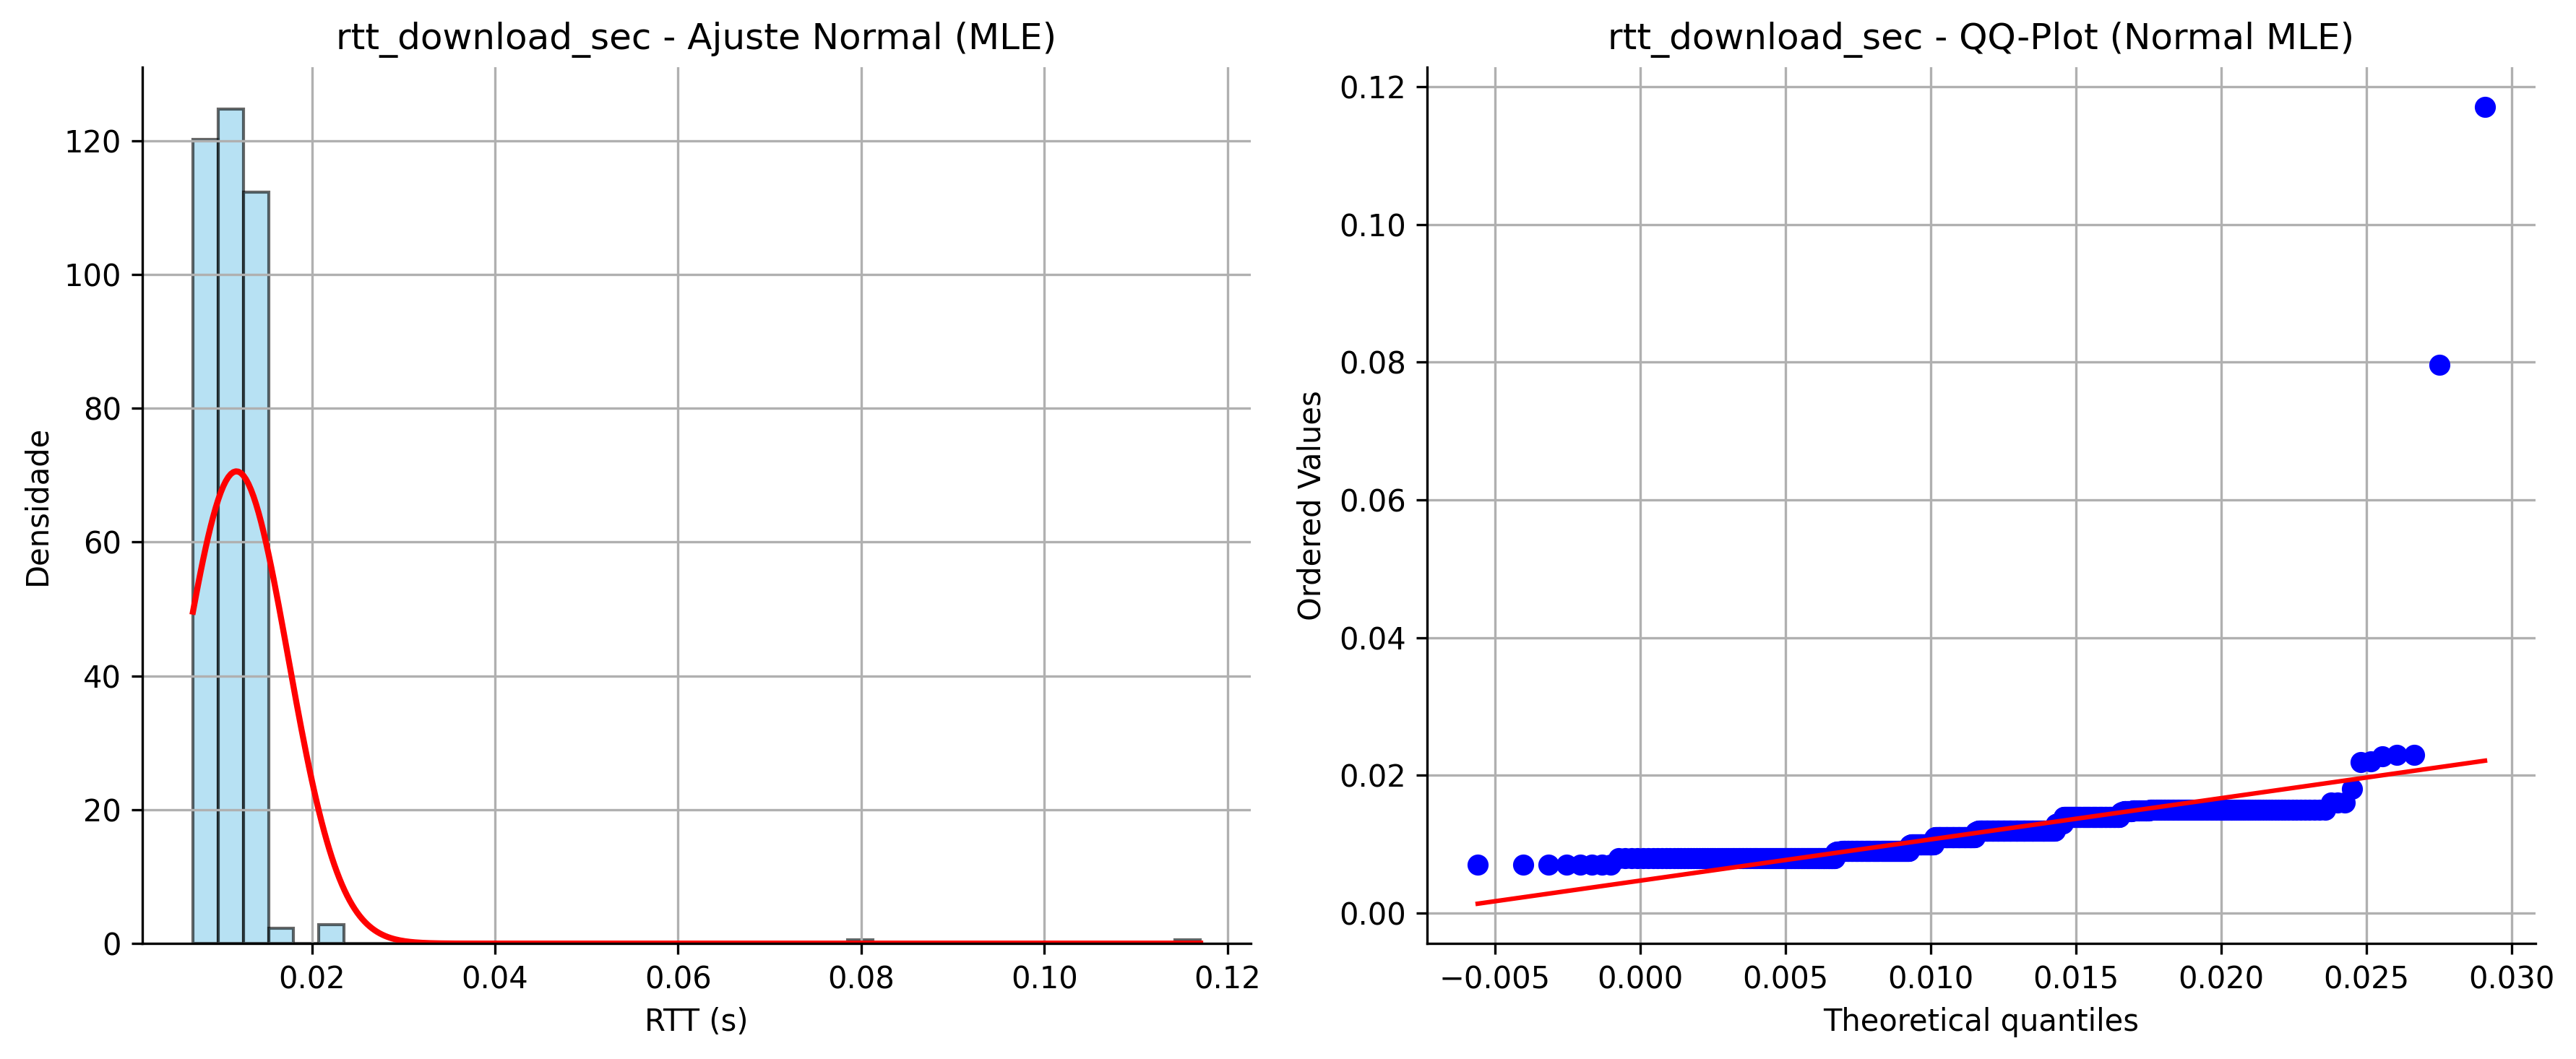
\includegraphics[width=\textwidth]{../figures/mle/rtt_download_sec_ajuste_normal_client13.png}
	\caption{Ajuste da distribuição Normal aos dados de RTT de download para o Cliente 13. À esquerda, histograma dos dados reais com a densidade teórica ajustada; à direita, gráfico QQ-plot comparando os quantis empíricos e teóricos.}
	\label{fig:rtt_download_sec_ajuste_normal_client13}
\end{figure}

\begin{figure}[htp]
	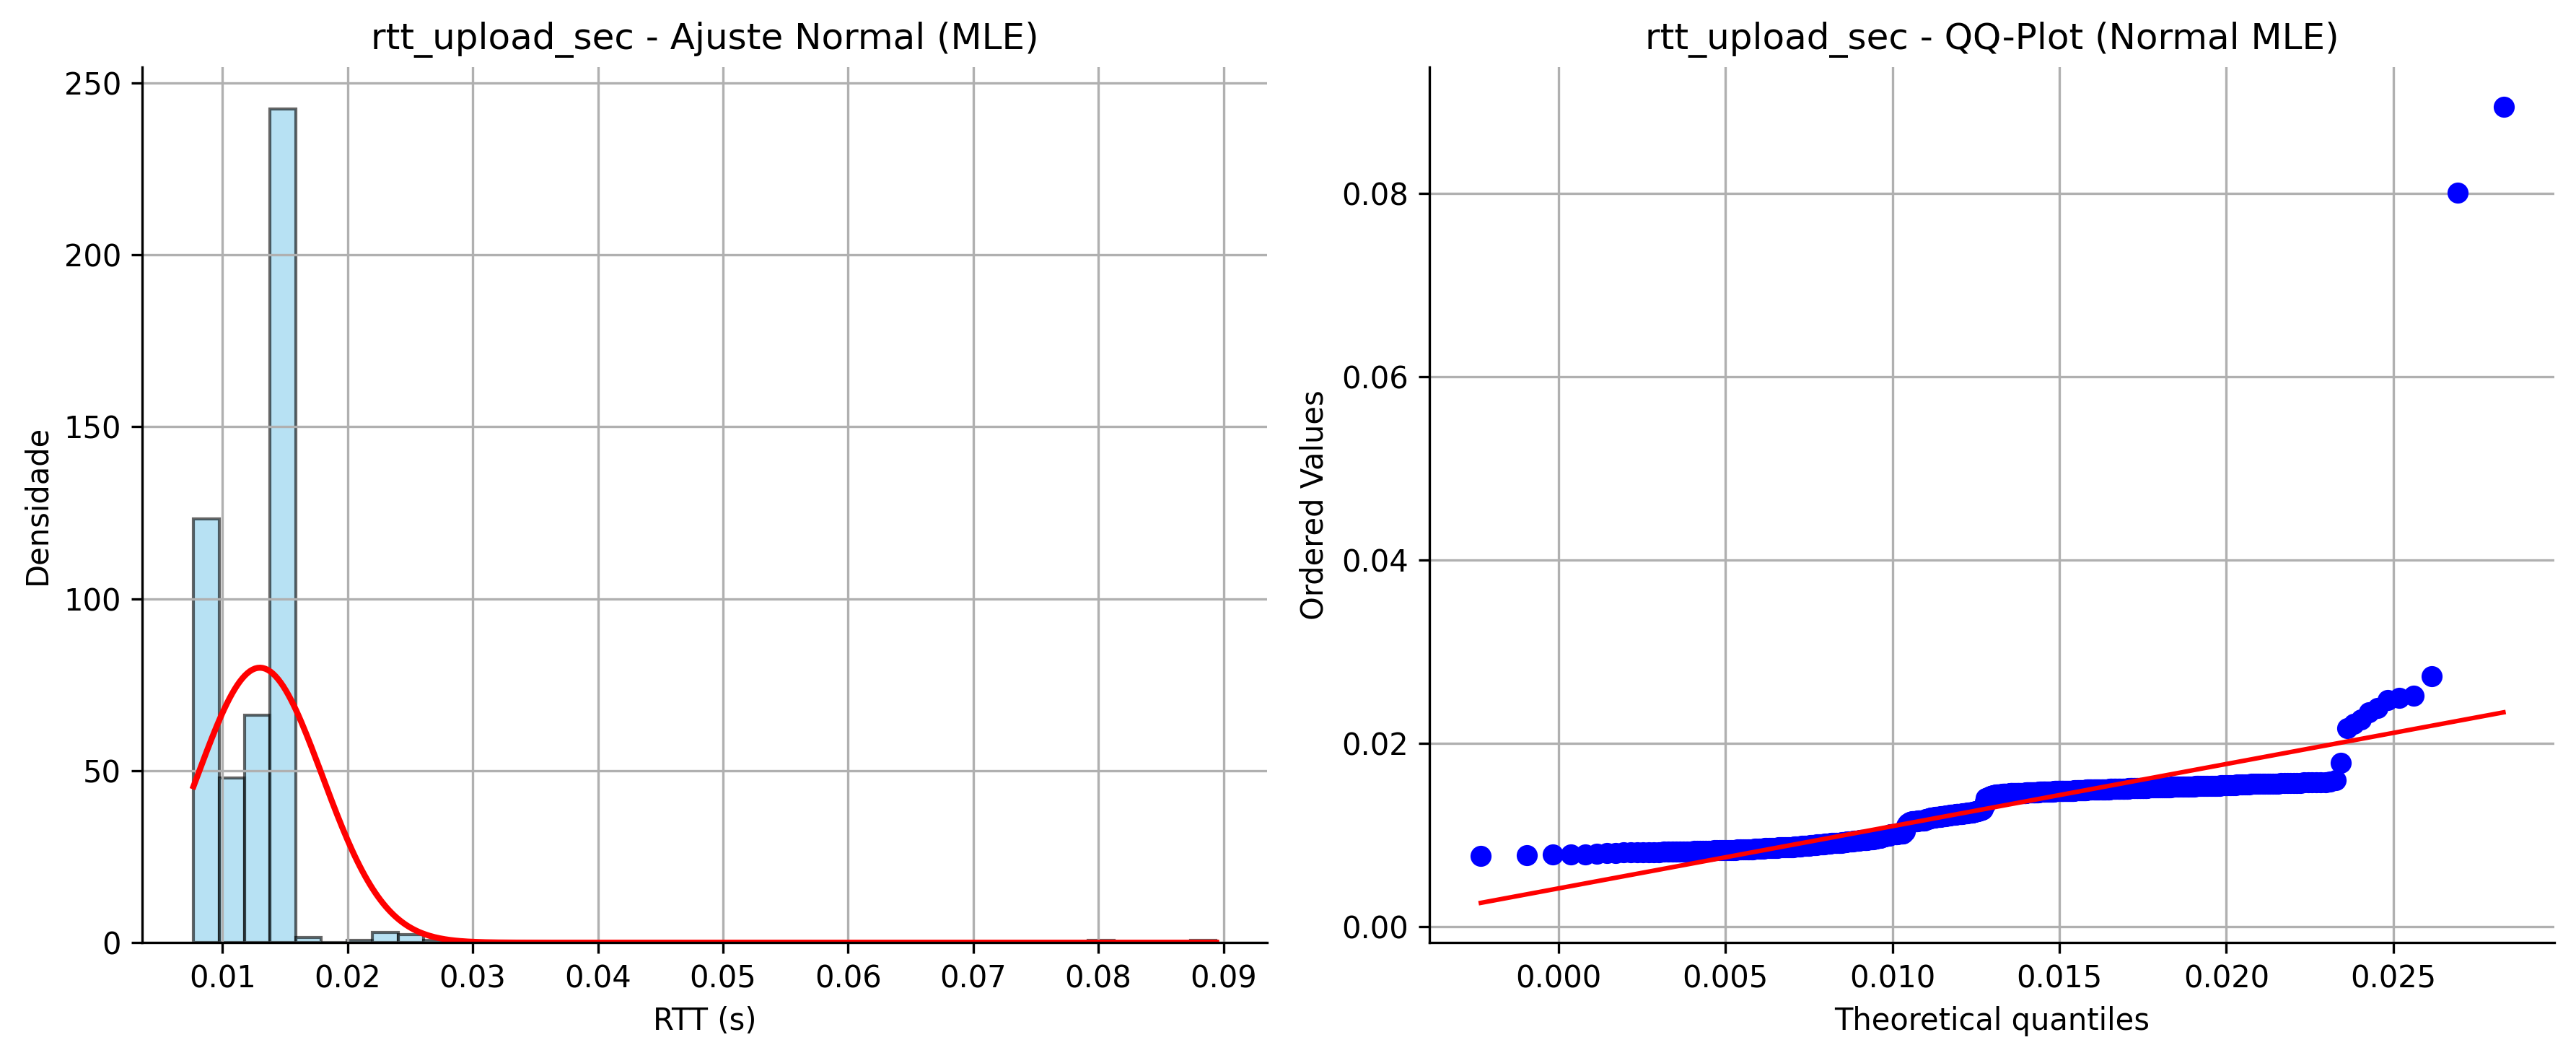
\includegraphics[width=\textwidth]{../figures/mle/rtt_upload_sec_ajuste_normal_client13.png}
	\caption{Ajuste da distribuição Normal aos dados de RTT de upload para o Cliente 13. O QQ-plot confirma a boa aderência do modelo à distribuição observada.}
	\label{fig:rtt_upload_sec_ajuste_normal_client13}
\end{figure}

\begin{figure}[htp]
	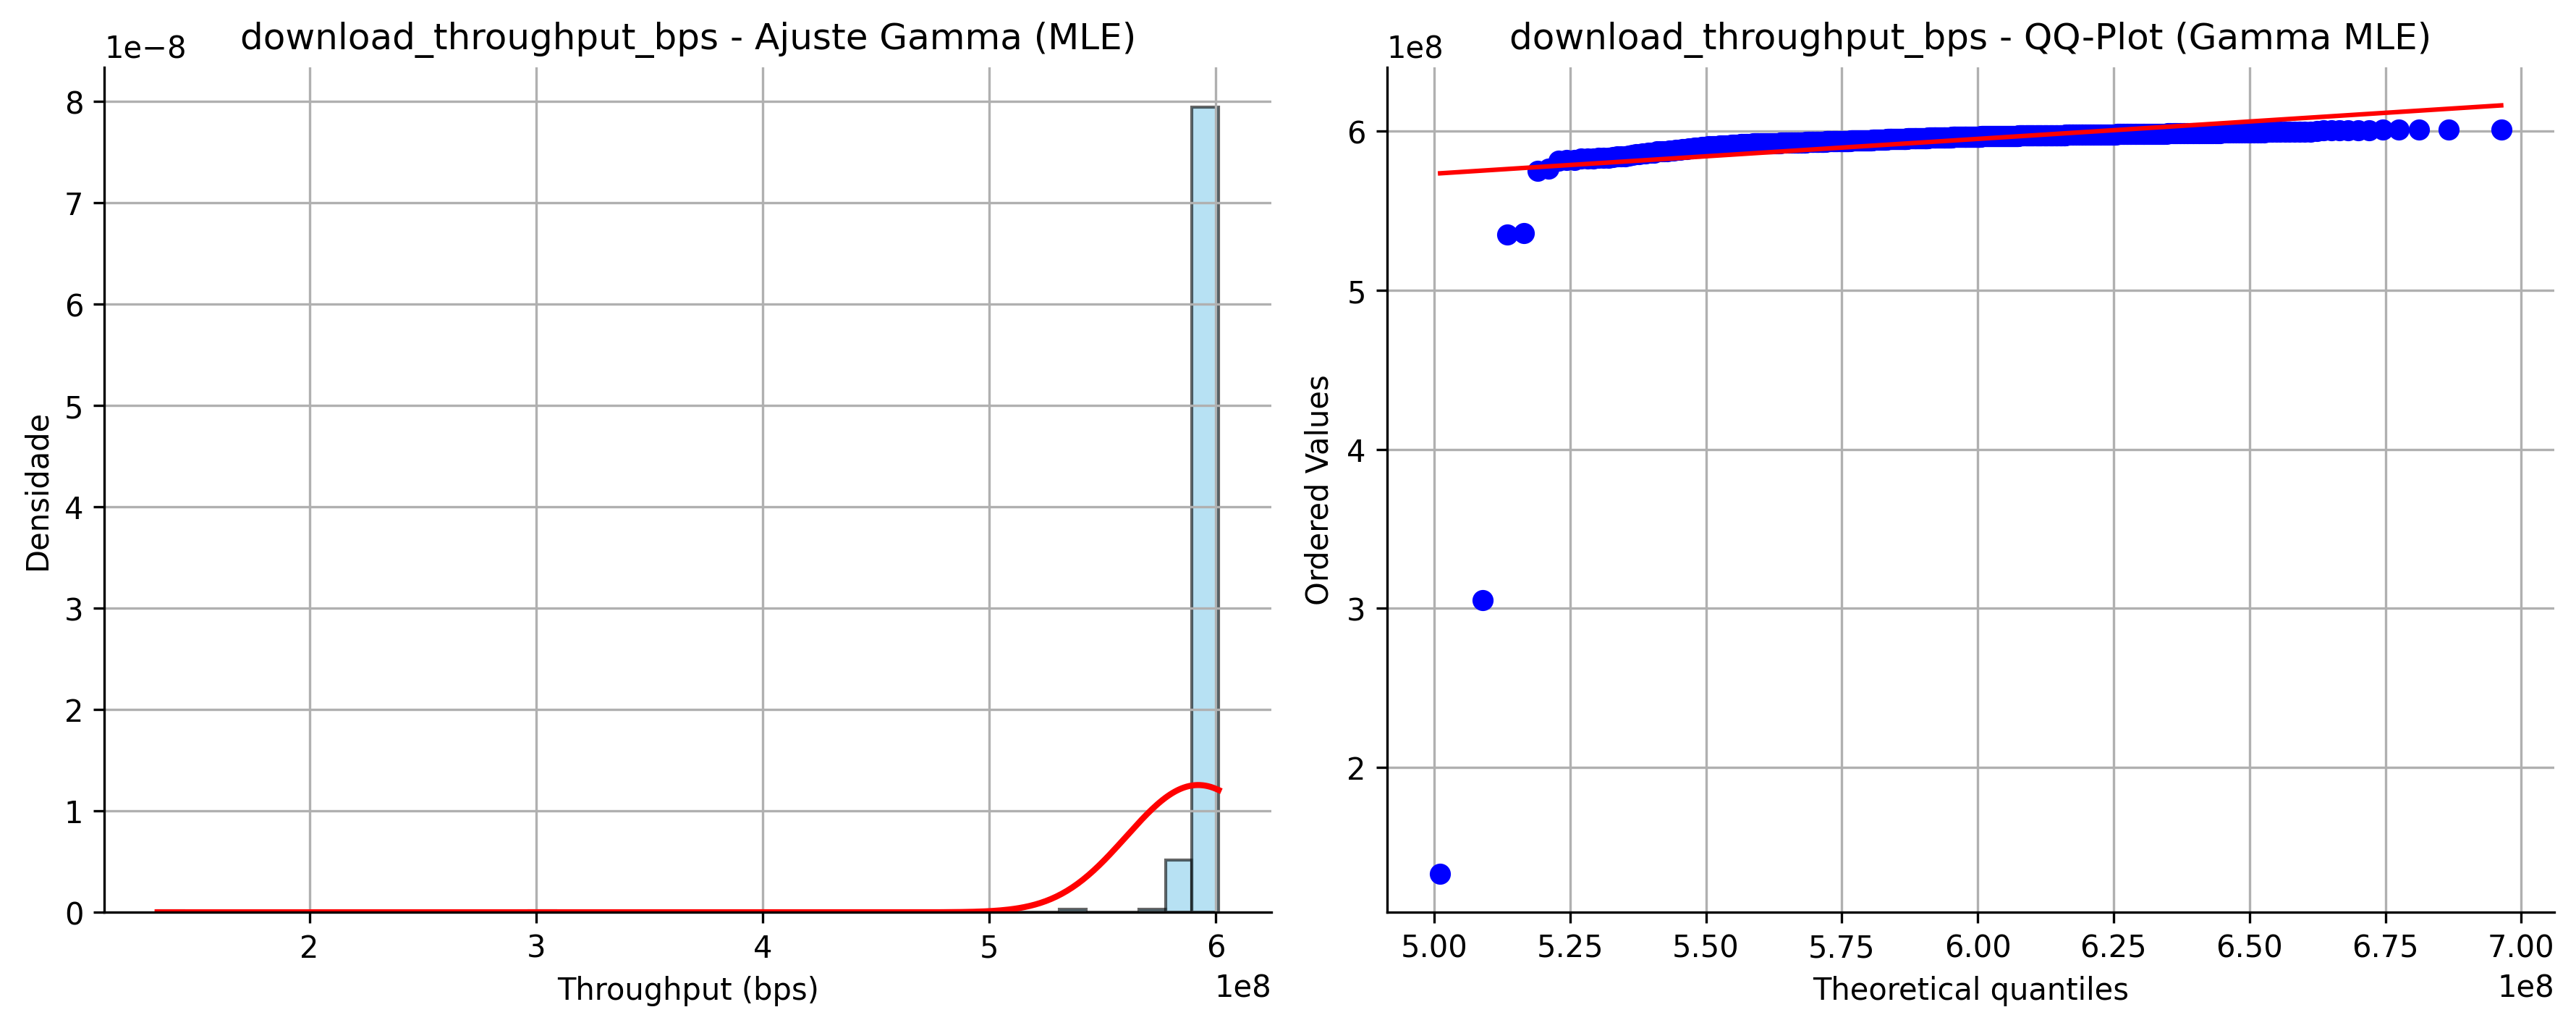
\includegraphics[width=\textwidth]{../figures/mle/download_throughput_bps_ajuste_gamma_client13.png}
	\caption{Ajuste da distribuição Gama aos dados de \textit{throughput} de download para o Cliente 13. O modelo representa bem a concentração principal dos dados, com pequenas discrepâncias nas caudas.}
	\label{fig:download_throughput_bps_ajuste_gamma_client13}
\end{figure}

\begin{figure}[htp]
	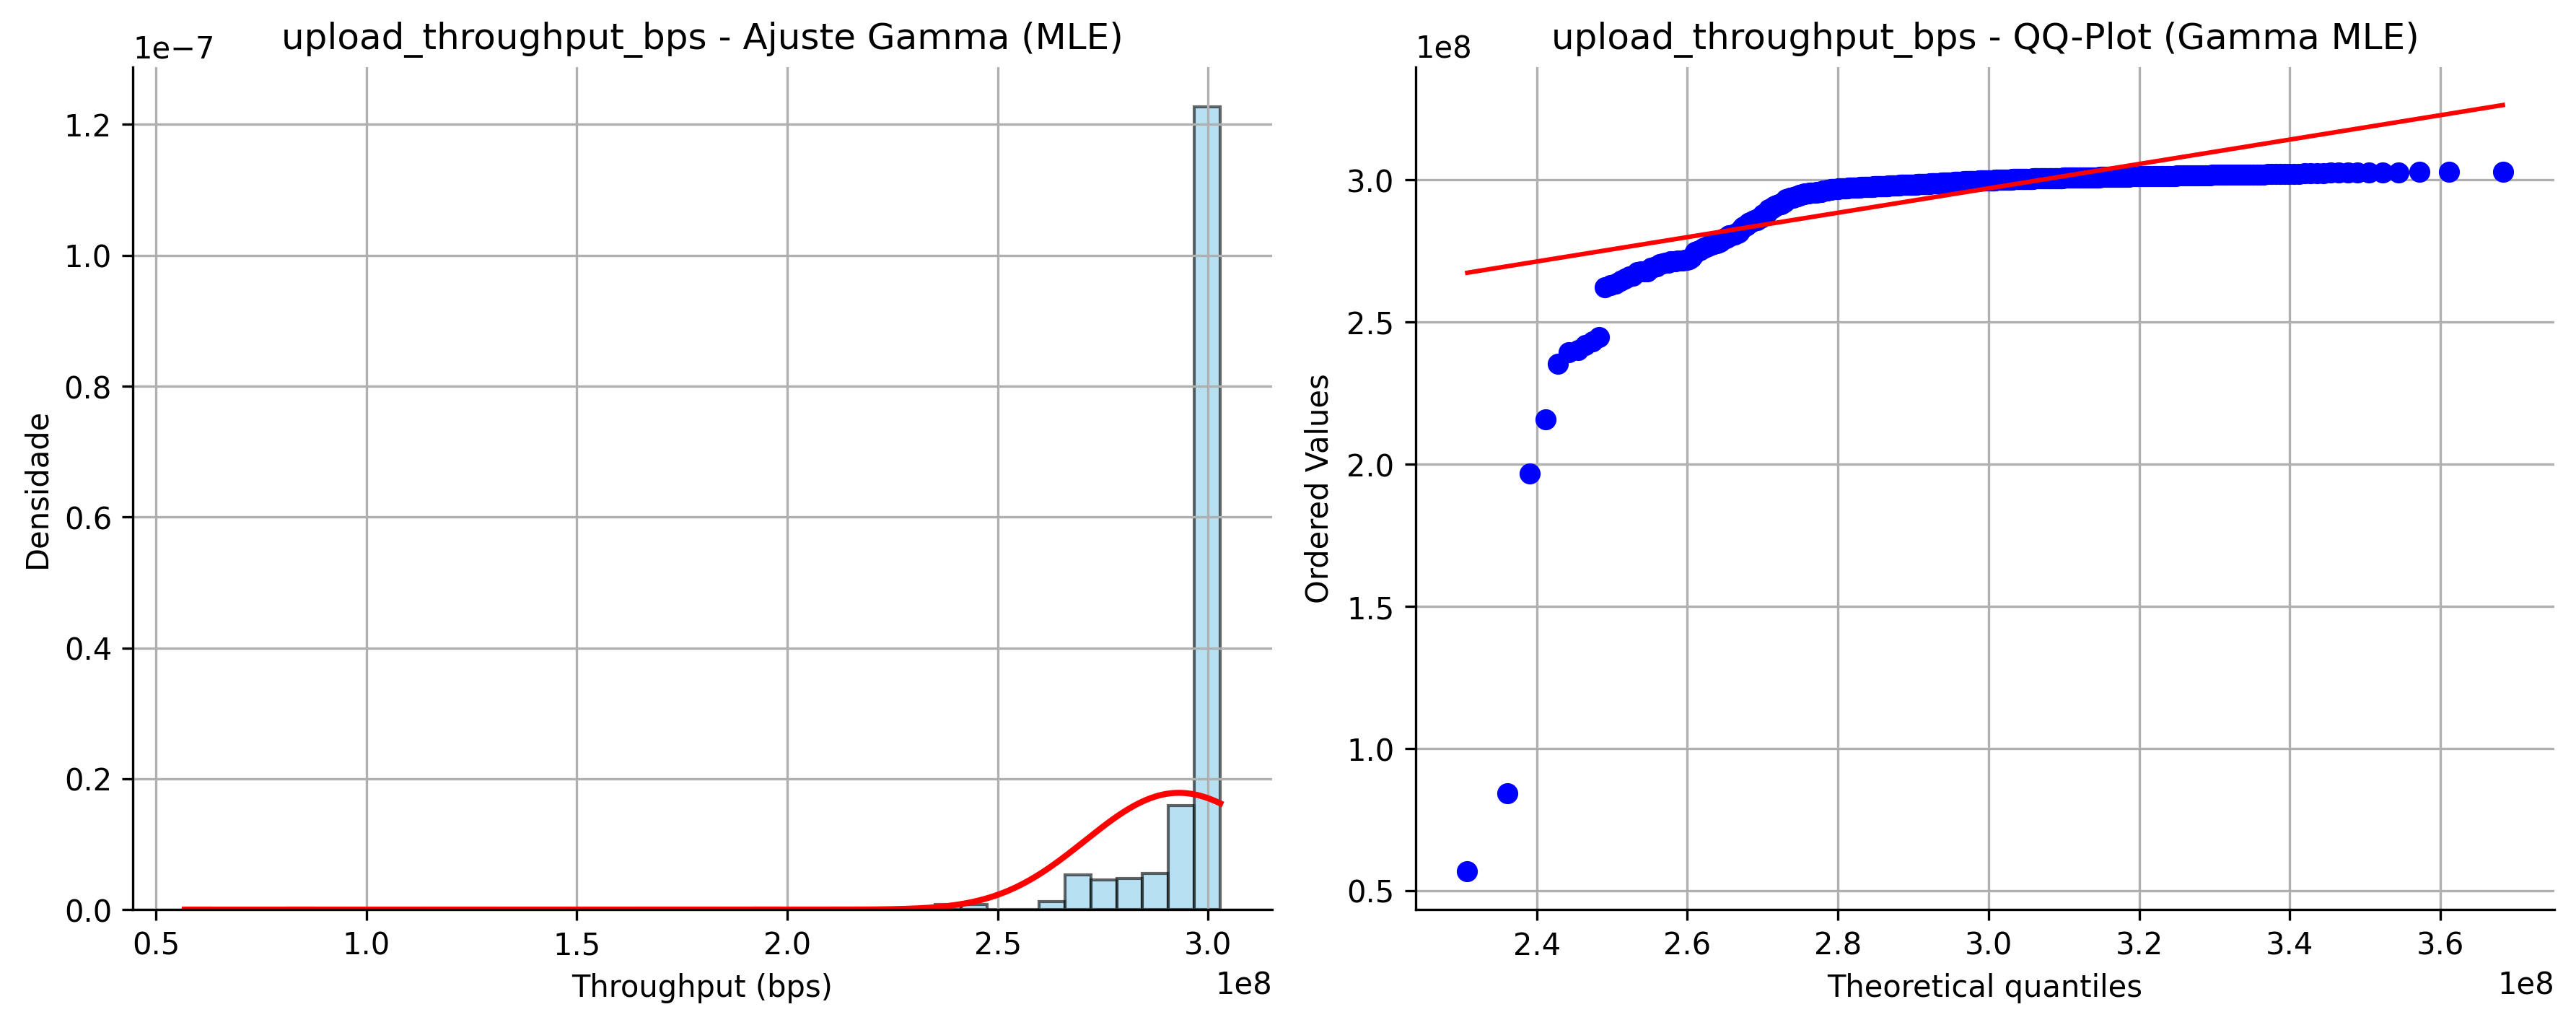
\includegraphics[width=\textwidth]{../figures/mle/upload_throughput_bps_ajuste_gamma_client13.png}
	\caption{Ajuste da distribuição Gama aos dados de \textit{throughput} de upload para o Cliente 13. Observa-se boa correspondência entre o modelo e a densidade empírica.}
	\label{fig:upload_throughput_bps_ajuste_gamma_client13}
\end{figure}

\begin{figure}[htp]
	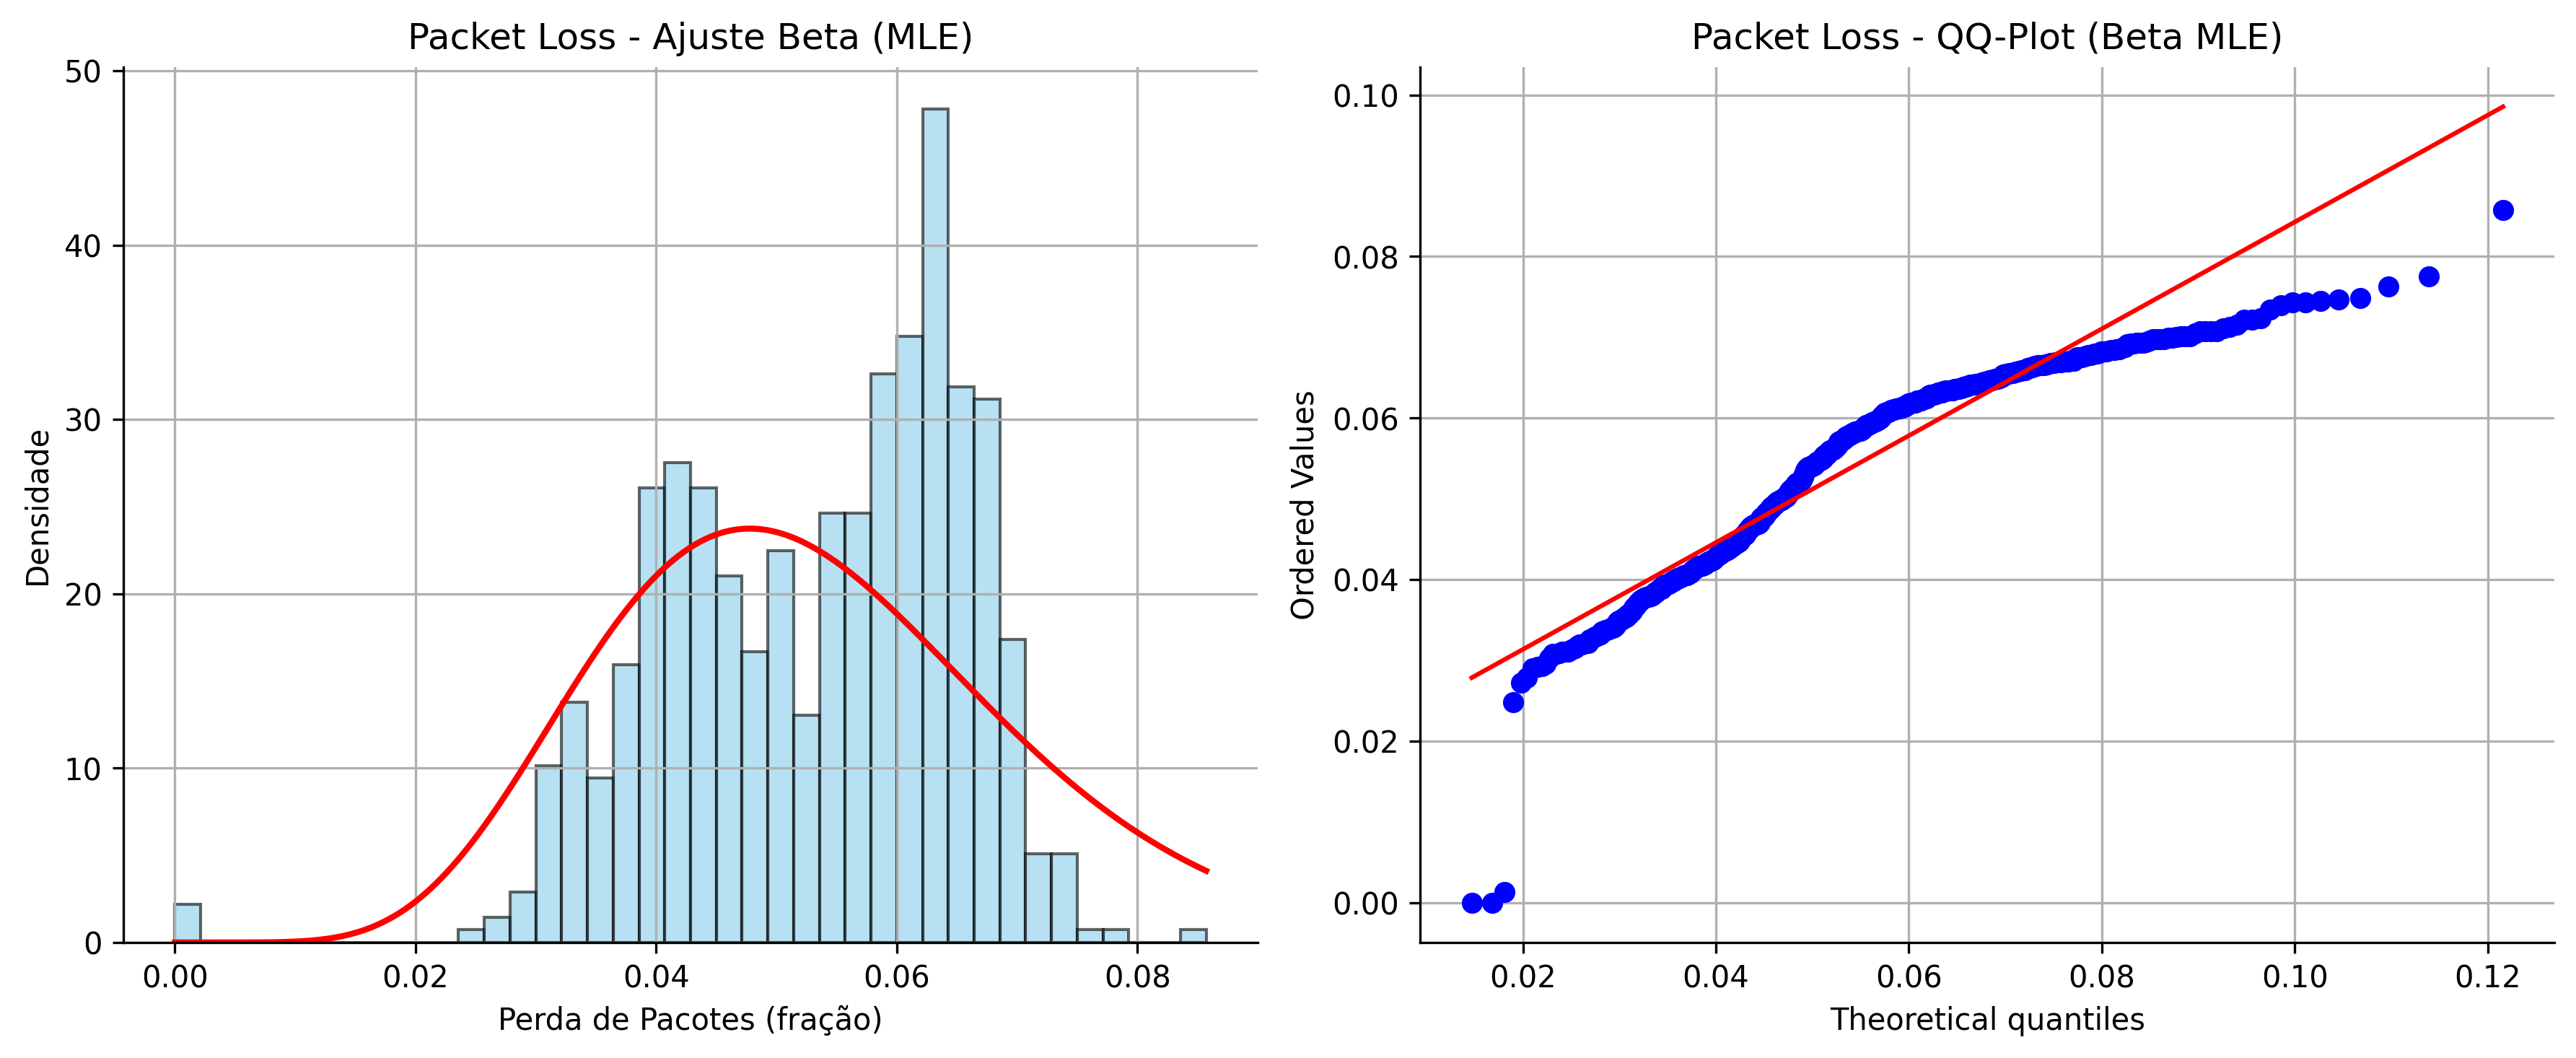
\includegraphics[width=\textwidth]{../figures/mle/packet_loss_ajuste_beta_client13.png}
	\caption{Ajuste da distribuição Beta à fração de perda de pacotes para o Cliente 13. O modelo descreve adequadamente a concentração de valores baixos observada nos dados.}
	\label{fig:packet_loss_ajuste_beta_client13}
\end{figure}

De forma geral, observa-se que todos os modelos apresentaram bom desempenho, a uma análise visual,
com as curvas ajustadas acompanhando de maneira satisfatória a forma das distribuições empíricas.
A consistência dos resultados é reforçada pelos \textit{QQ-plots}, nos quais os pontos seguem
aproximadamente a linha de referência, indicando que os quantis teóricos e empíricos são compatíveis.

Pequenas divergências podem ser notadas nas extremidades dos histogramas, especialmente nas caudas
das distribuições, sugerindo uma leve sub-representação dos valores extremos.
Essas discrepâncias, contudo, são esperadas e podem estar associadas à presença de \textit{outliers}
ou à própria natureza estocástica dos fenômenos observados, uma vez que a maior parte das observações
se concentra em faixas bem delimitadas, o que reforça a qualidade geral do ajuste.

Para avaliar a interação entre os parâmetros e verificar o ponto de máximo global de verossimilhança,
foram gerados mapas de calor (\textit{heatmaps}) da log-verossimilhança.
As Figuras~\ref{fig:rtt_loglik_normal_combined}, \ref{fig:throughput_gamma_loglik_combined}
e \ref{fig:packet_loss_loglik_surface_beta_client13} apresentam essas superfícies,
nas quais o ponto de máximo identifica o par de parâmetros que melhor descreve os dados.
O uso da log-verossimilhança se justifica pela sua maior estabilidade numérica
e pela simplificação do produto em somas, o que facilita a localização do máximo.

\begin{figure}[htp]
	\centering
	% Subfigure 1
	\begin{subfigure}[b]{0.48\textwidth} % Ocupa 48% da largura do texto
		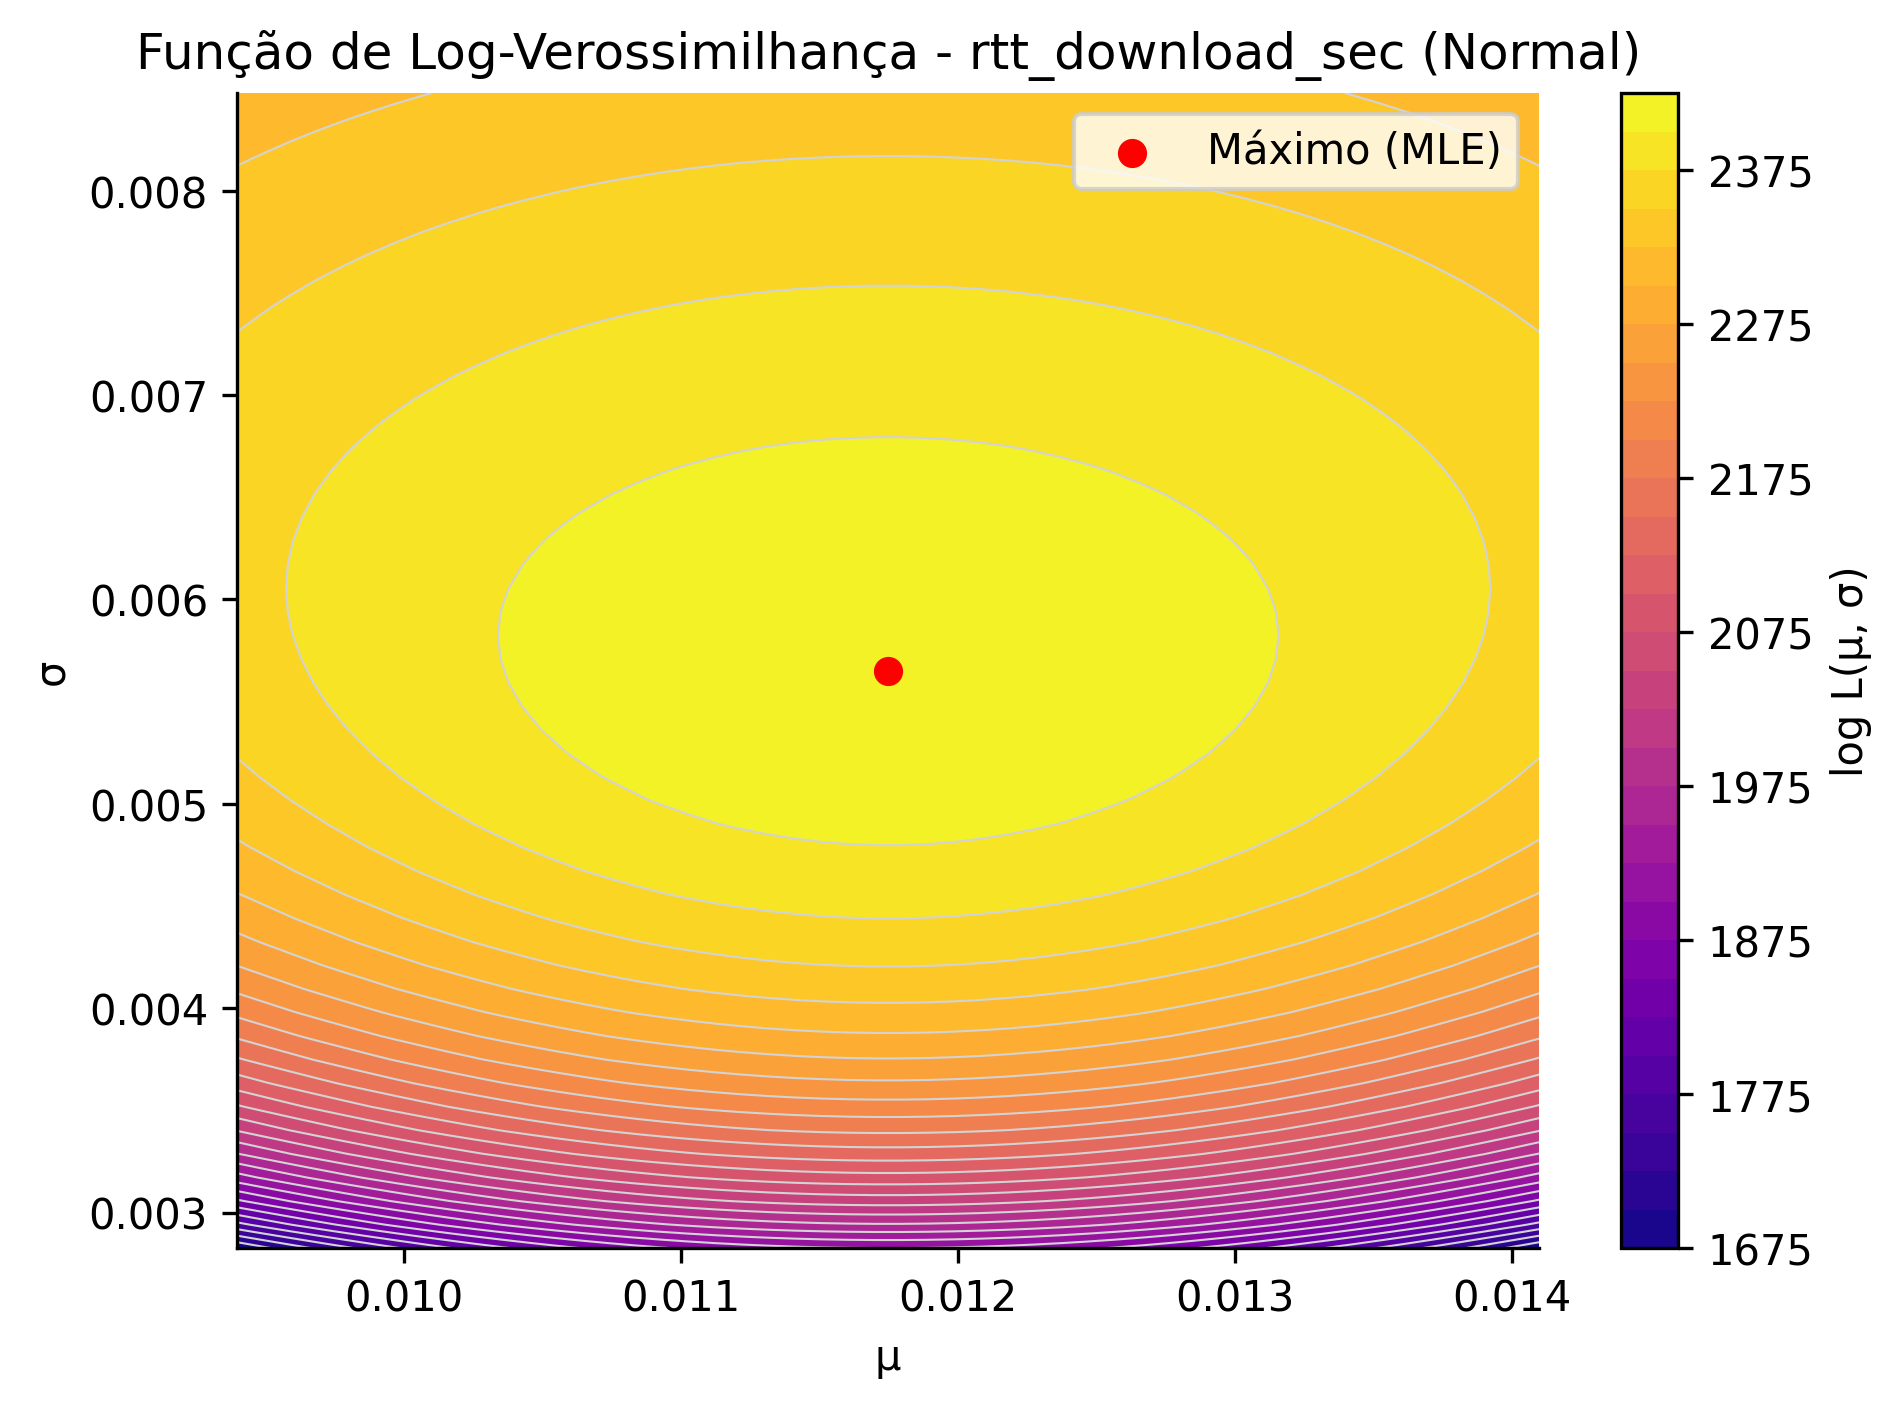
\includegraphics[width=\textwidth]{../figures/mle/rtt_download_sec_loglik_surface_normal_client13.png}
		\caption{RTT Download (Normal)}
		\label{fig:rtt_download_sec_loglik_surface_normal_client13}
	\end{subfigure}
	\hfill % Espaço horizontal entre as subfiguras
	% Subfigure 2
	\begin{subfigure}[b]{0.48\textwidth} % Ocupa 48% da largura do texto
		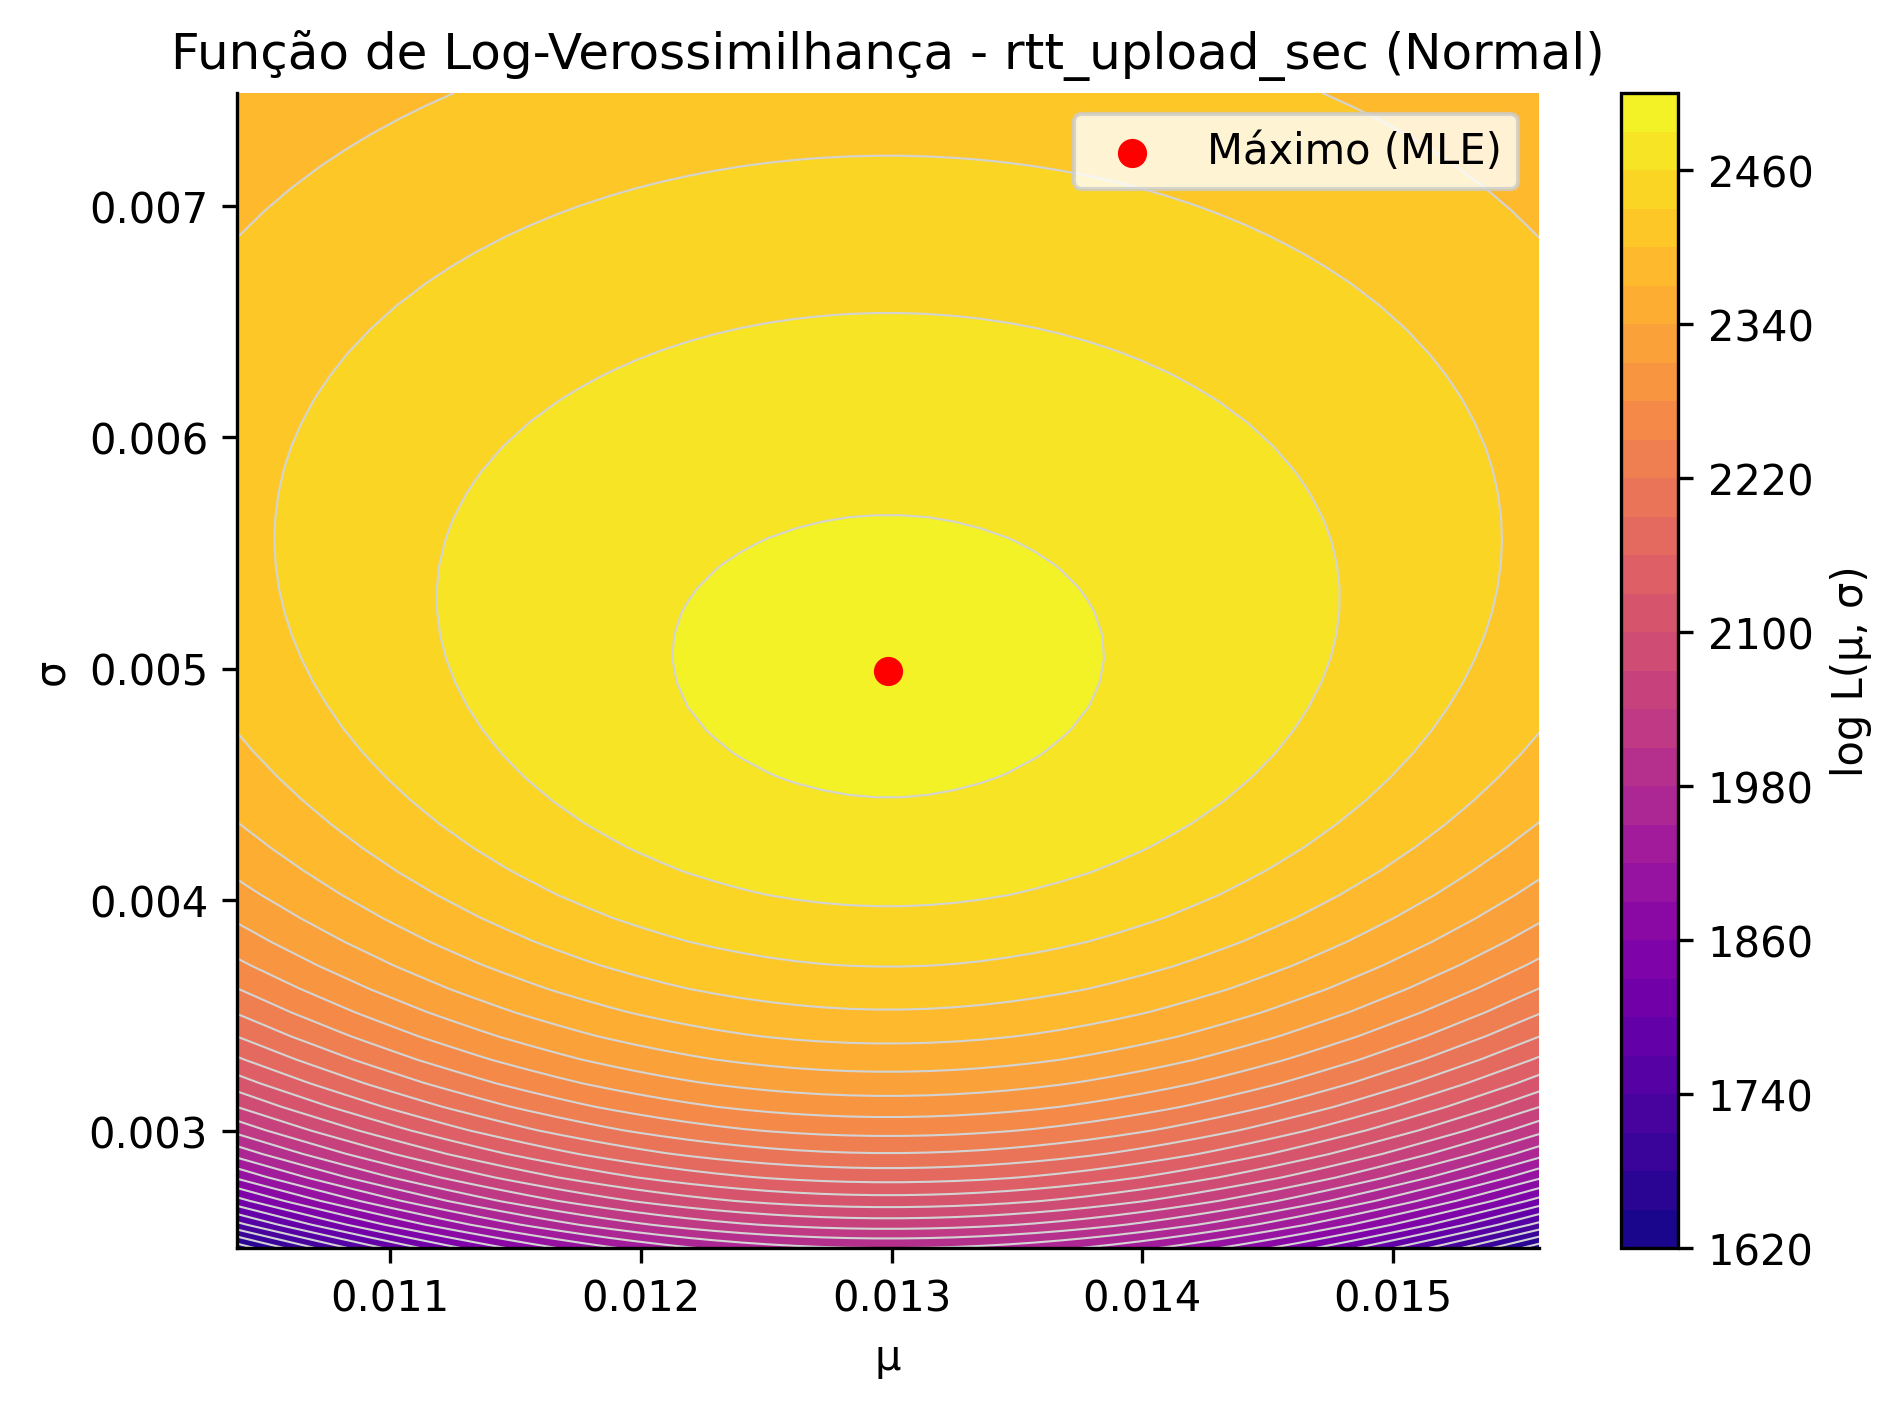
\includegraphics[width=\textwidth]{../figures/mle/rtt_upload_sec_loglik_surface_normal_client13.png}
		\caption{RTT Upload (Normal)}
		\label{fig:rtt_upload_sec_loglik_surface_normal_client13}
	\end{subfigure}
	\caption{Superfícies de log-verossimilhança para os parâmetros $\mu$ e $\sigma$ da distribuição Normal (RTT de download e upload) do Cliente 13. O ponto de máximo indica o par de parâmetros que melhor descreve os dados.}
	\label{fig:rtt_loglik_normal_combined}
\end{figure}

\begin{figure}[htp]
	\centering
	\begin{subfigure}[b]{0.48\textwidth} % Ocupa 48% da largura do texto
		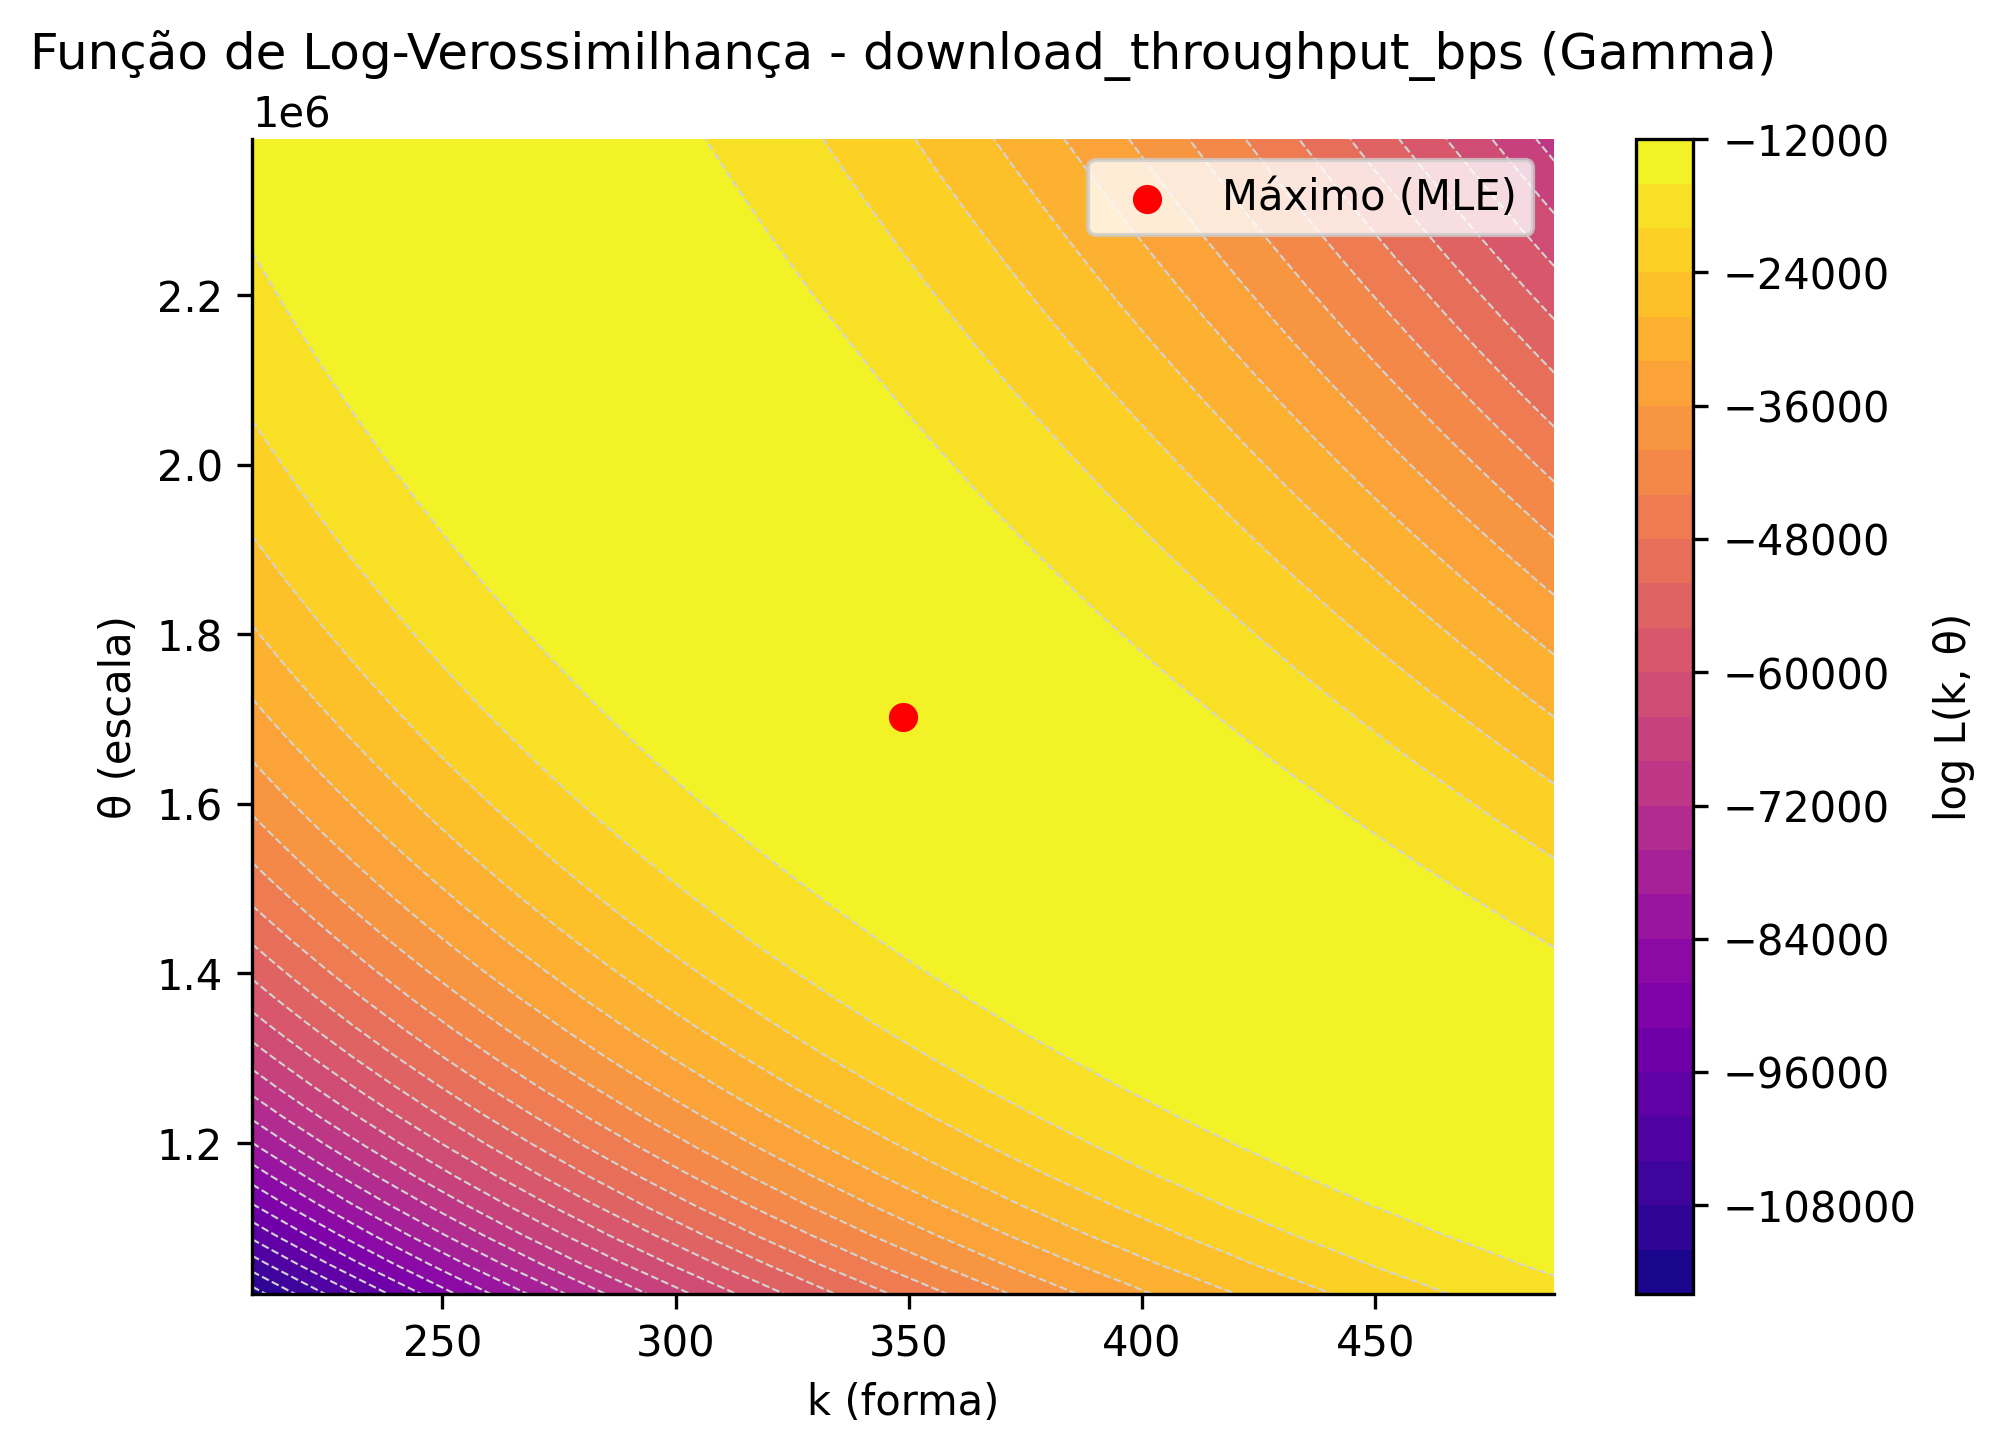
\includegraphics[width=\textwidth]{../figures/mle/download_throughput_bps_loglik_surface_gamma_client13.png}
		\caption{Throughput de Download (Distribuição Gamma)}
		\label{fig:download_throughput_bps_loglik_surface_gamma_client13}
	\end{subfigure}
	\hfill 
	\begin{subfigure}[b]{0.48\textwidth}
		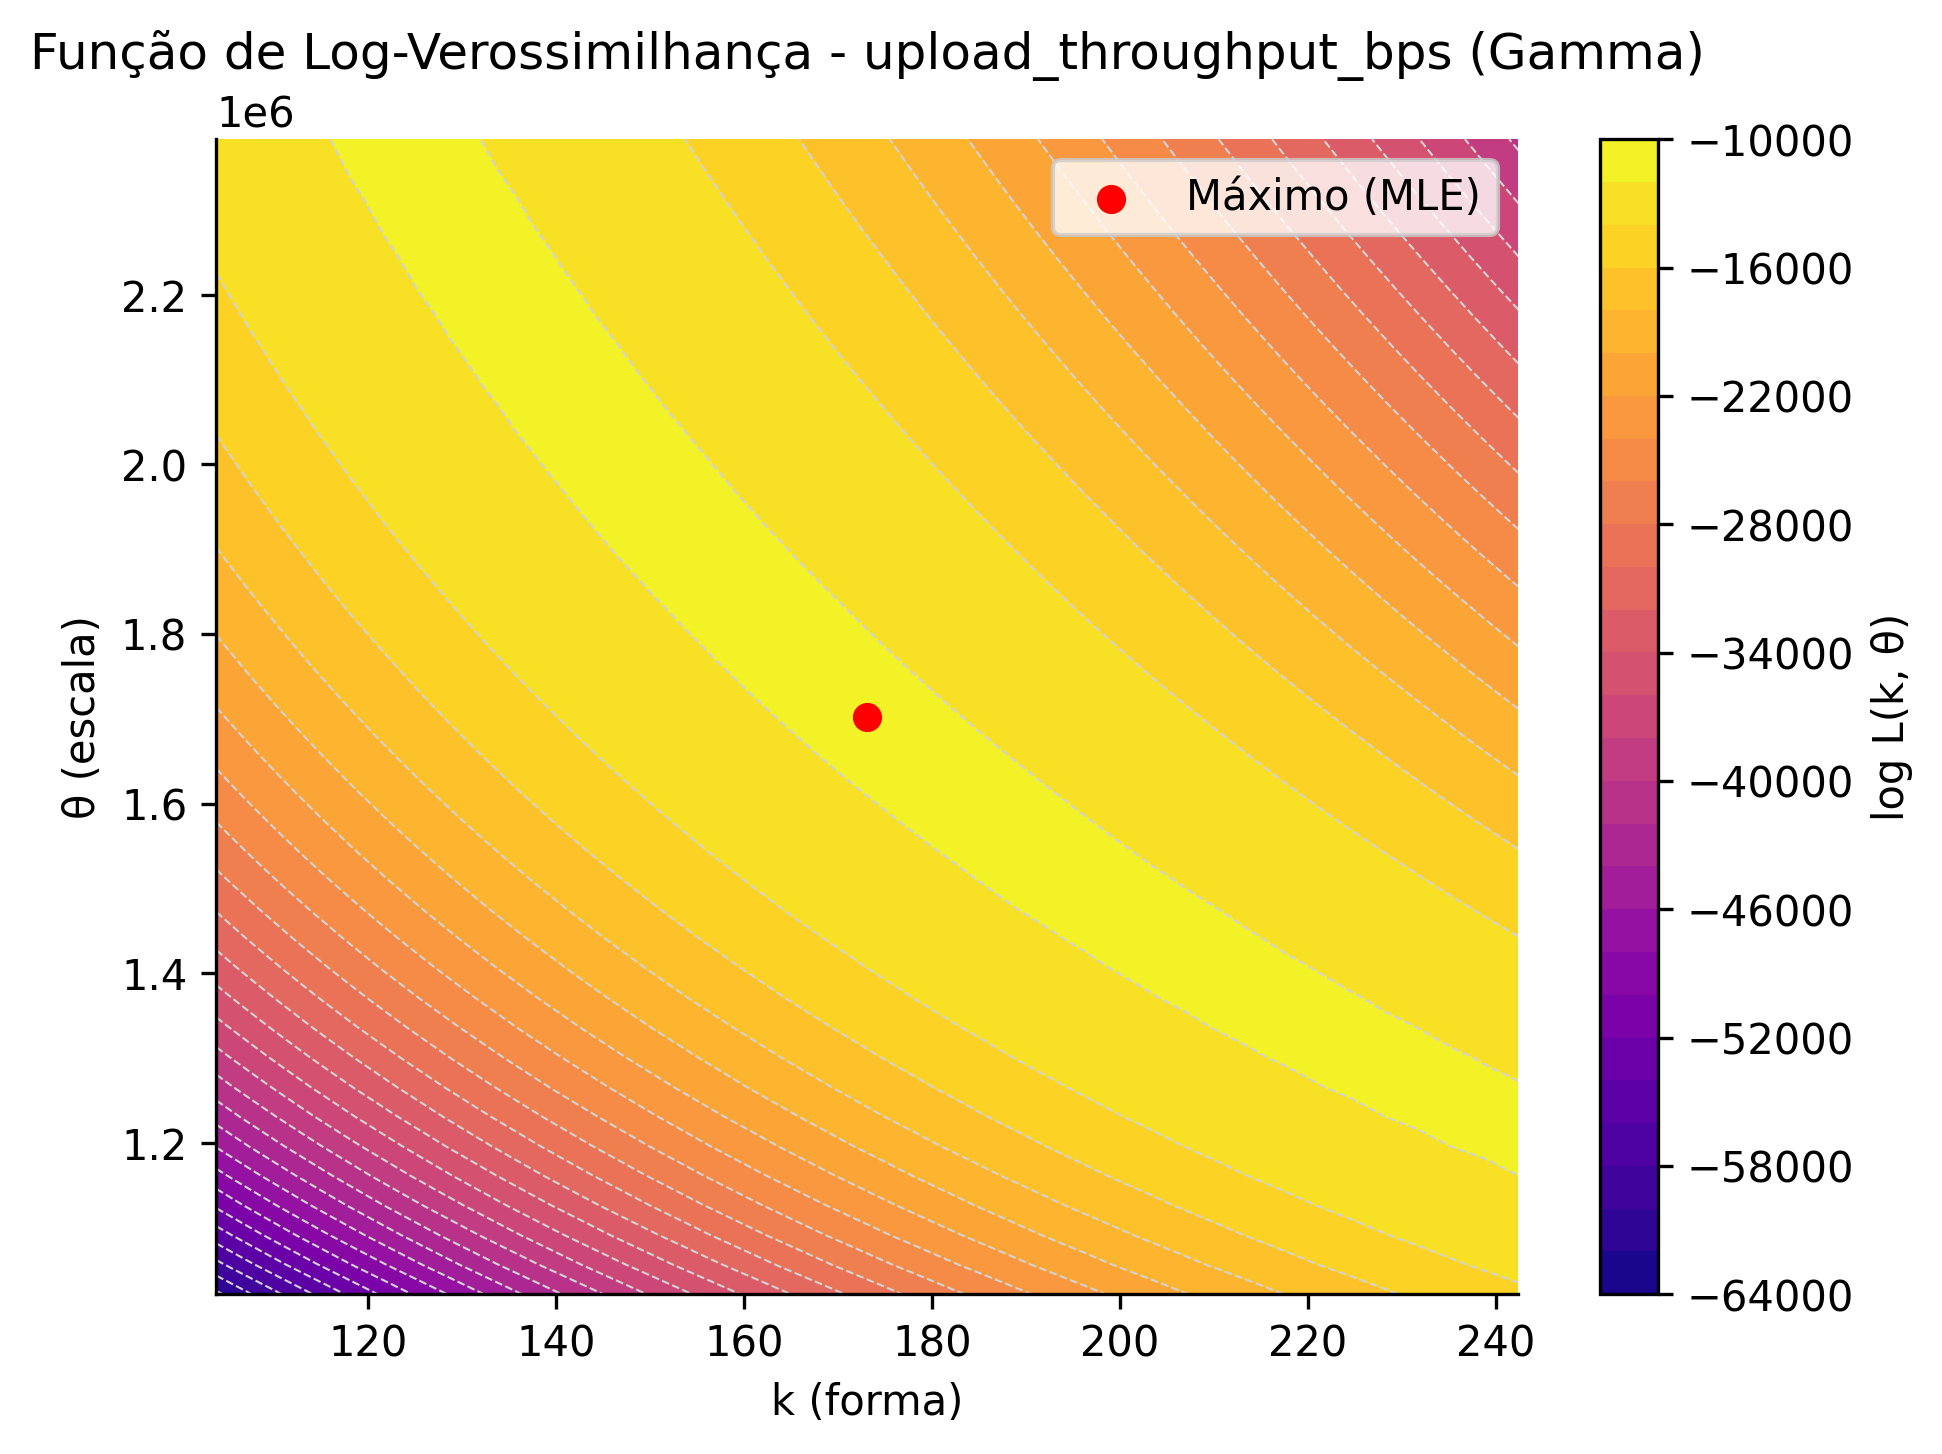
\includegraphics[width=\textwidth]{../figures/mle/upload_throughput_bps_loglik_surface_gamma_client13.png}
		\caption{Throughput de Upload (Distribuição Gamma)}
		\label{fig:upload_throughput_bps_loglik_surface_gamma_client13}
	\end{subfigure}
	\caption{Superfícies de log-verossimilhança para os parâmetros $k$ e $\theta$ da distribuição Gama aplicada às variáveis de \textit{throughput} (download e upload) do Cliente 13.}
	\label{fig:throughput_gamma_loglik_combined}
\end{figure}

\begin{figure}[htp]
	\centering
	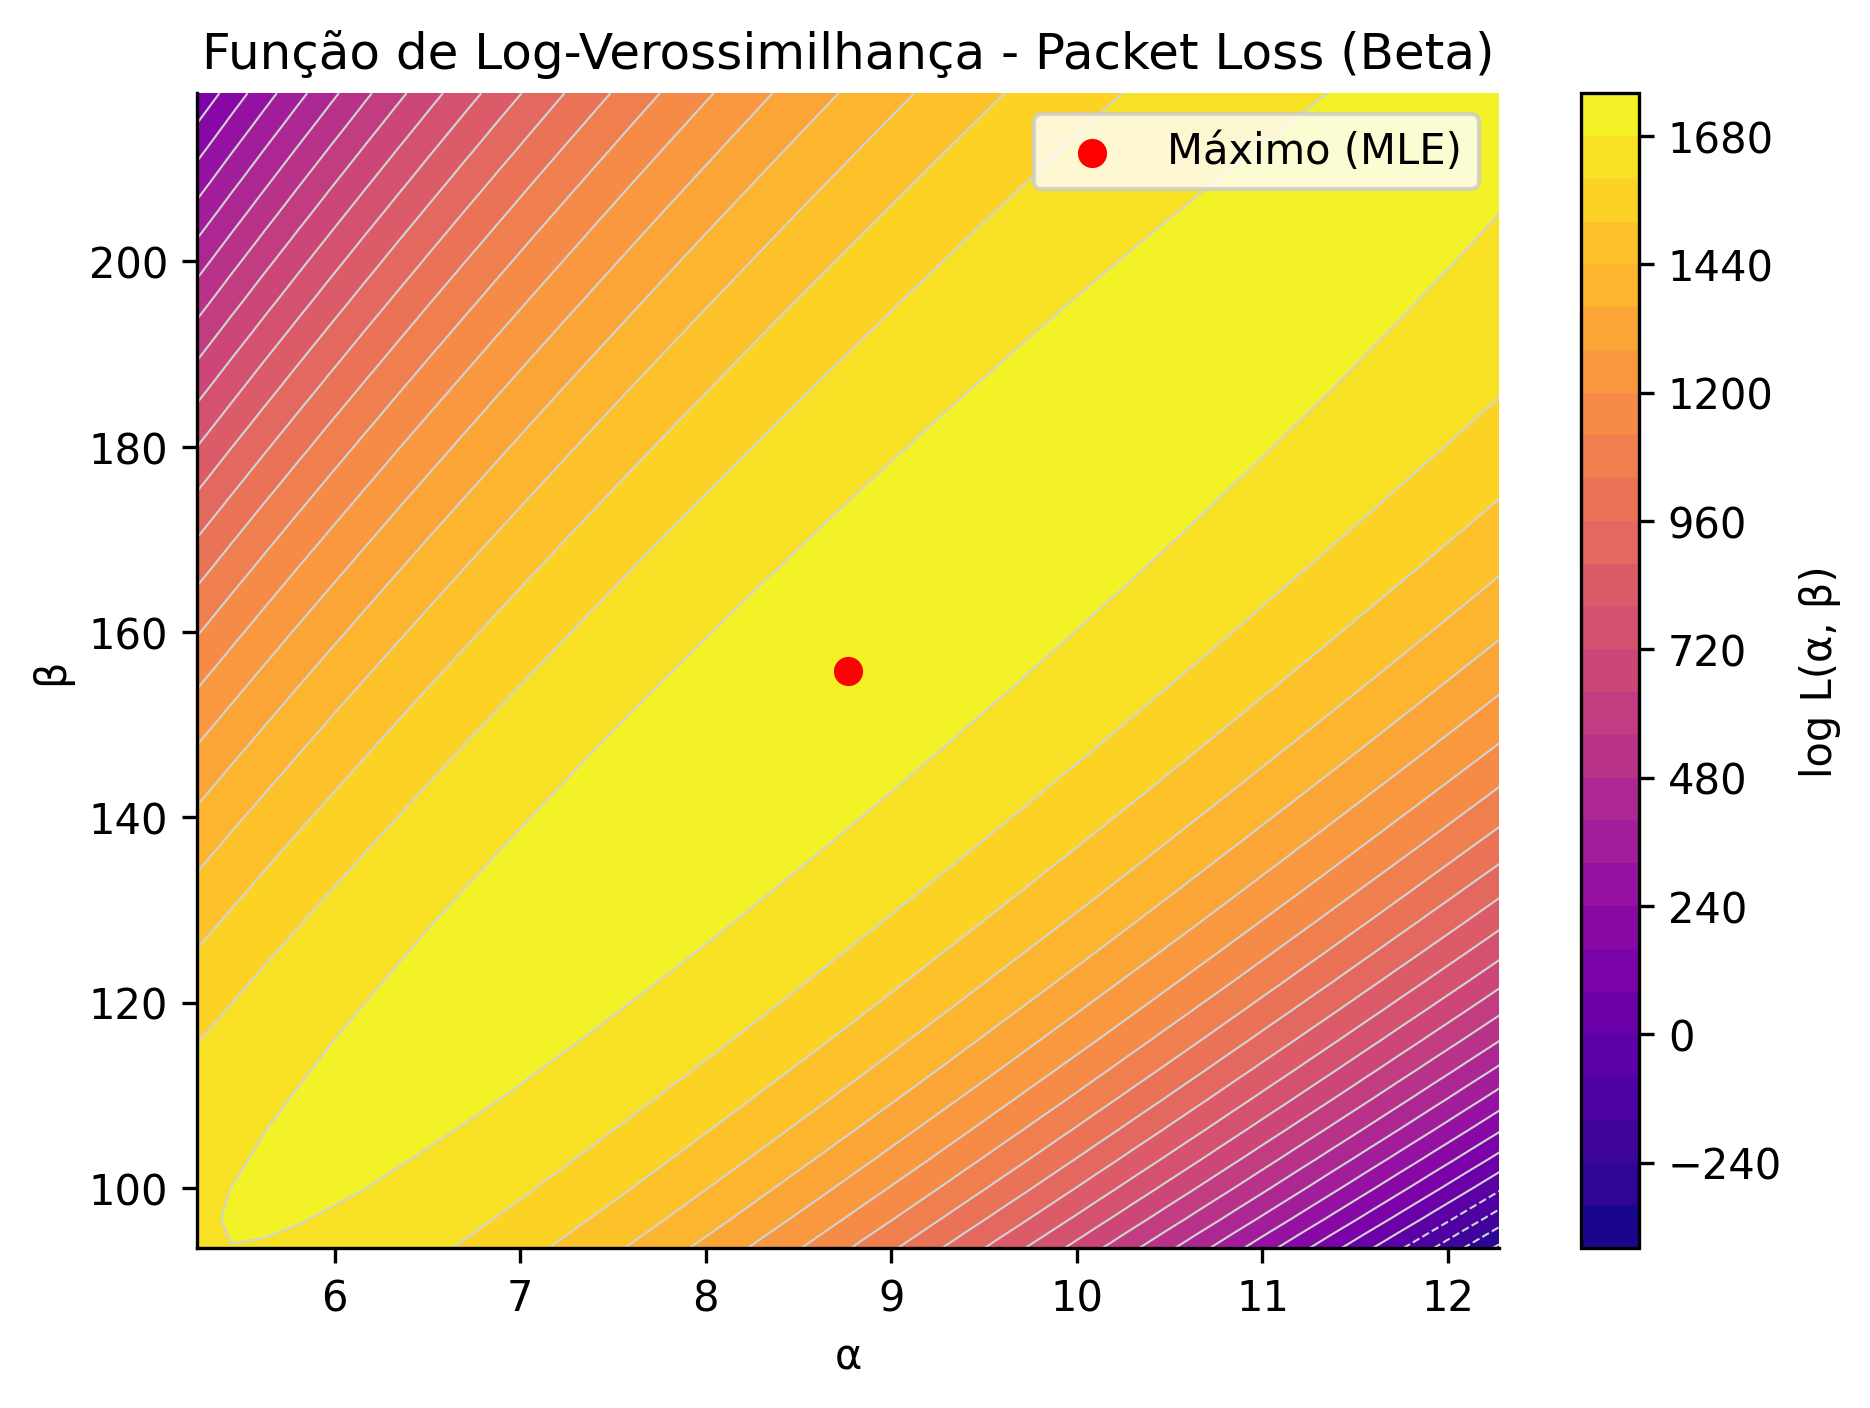
\includegraphics[width=0.48\textwidth]{../figures/mle/packet_loss_loglik_surface_beta_client13.png}
	\caption{Superfície de log-verossimilhança para os parâmetros $\alpha$ e $\beta$ da distribuição Beta ajustada à variável de perda de pacotes do Cliente 13.}
	\label{fig:packet_loss_loglik_surface_beta_client13}
\end{figure}

Por fim, a Tabela~\ref{tab:mle_parameters_client13} apresenta os valores finais estimados para cada variável,
representando o conjunto de parâmetros $\hat{\boldsymbol{\theta}}_{MLE}$ que maximiza a verossimilhança
do modelo ajustado para o Cliente 13.

\begin{table}[htp]
	\centering
	\caption{Parâmetros estimados por Máxima Verossimilhança (MLE) para o Cliente 13. Os valores correspondem aos estimadores que maximizam a função de verossimilhança de cada modelo ajustado.}
	\label{tab:mle_parameters_client13}
	\begin{tabular}{|l|c|l|}
		\hline
		\textbf{Variável} & \textbf{Distribuição} & \textbf{Parâmetros MLE}\\
		\hline
		rtt\_download\_sec & Normal & $\hat{\mu}=0.01175$, $\hat{\sigma}=0.005652$\\
		\hline
		rtt\_upload\_sec & Normal & $\hat{\mu}=0.01299$, $\hat{\sigma}=0.004991$\\
		\hline
		download\_throughput\_bps & Gamma & $\hat{k}=348.8$, $\hat{\theta}=1.703 \times 10^6$ \\
		\hline
		upload\_throughput\_bps & Gamma & $\hat{k}=173.1$, $\hat{\theta}=1.703 \times 10^6$ \\
		\hline
		packet\_loss\_percent & Beta & $\hat{\alpha}=8.769$, $\hat{\beta}=155.8$ \\
		\hline
	\end{tabular}
\end{table}

\subsubsection*{Resultados para o Servidor 02}

De forma análoga ao caso anterior, as Figuras~\ref{fig:rtt_download_sec_ajuste_normal_server02}
a \ref{fig:packet_loss_ajuste_beta_serve02} apresentam os resultados obtidos
para o Servidor 02. Observa-se novamente que os modelos normais e beta obtiveram
bom desempenho, especialmente para as variáveis de RTT e perda de pacotes,
cuja distribuição empírica é bem descrita pelos modelos propostos.

\begin{figure}[htp]
	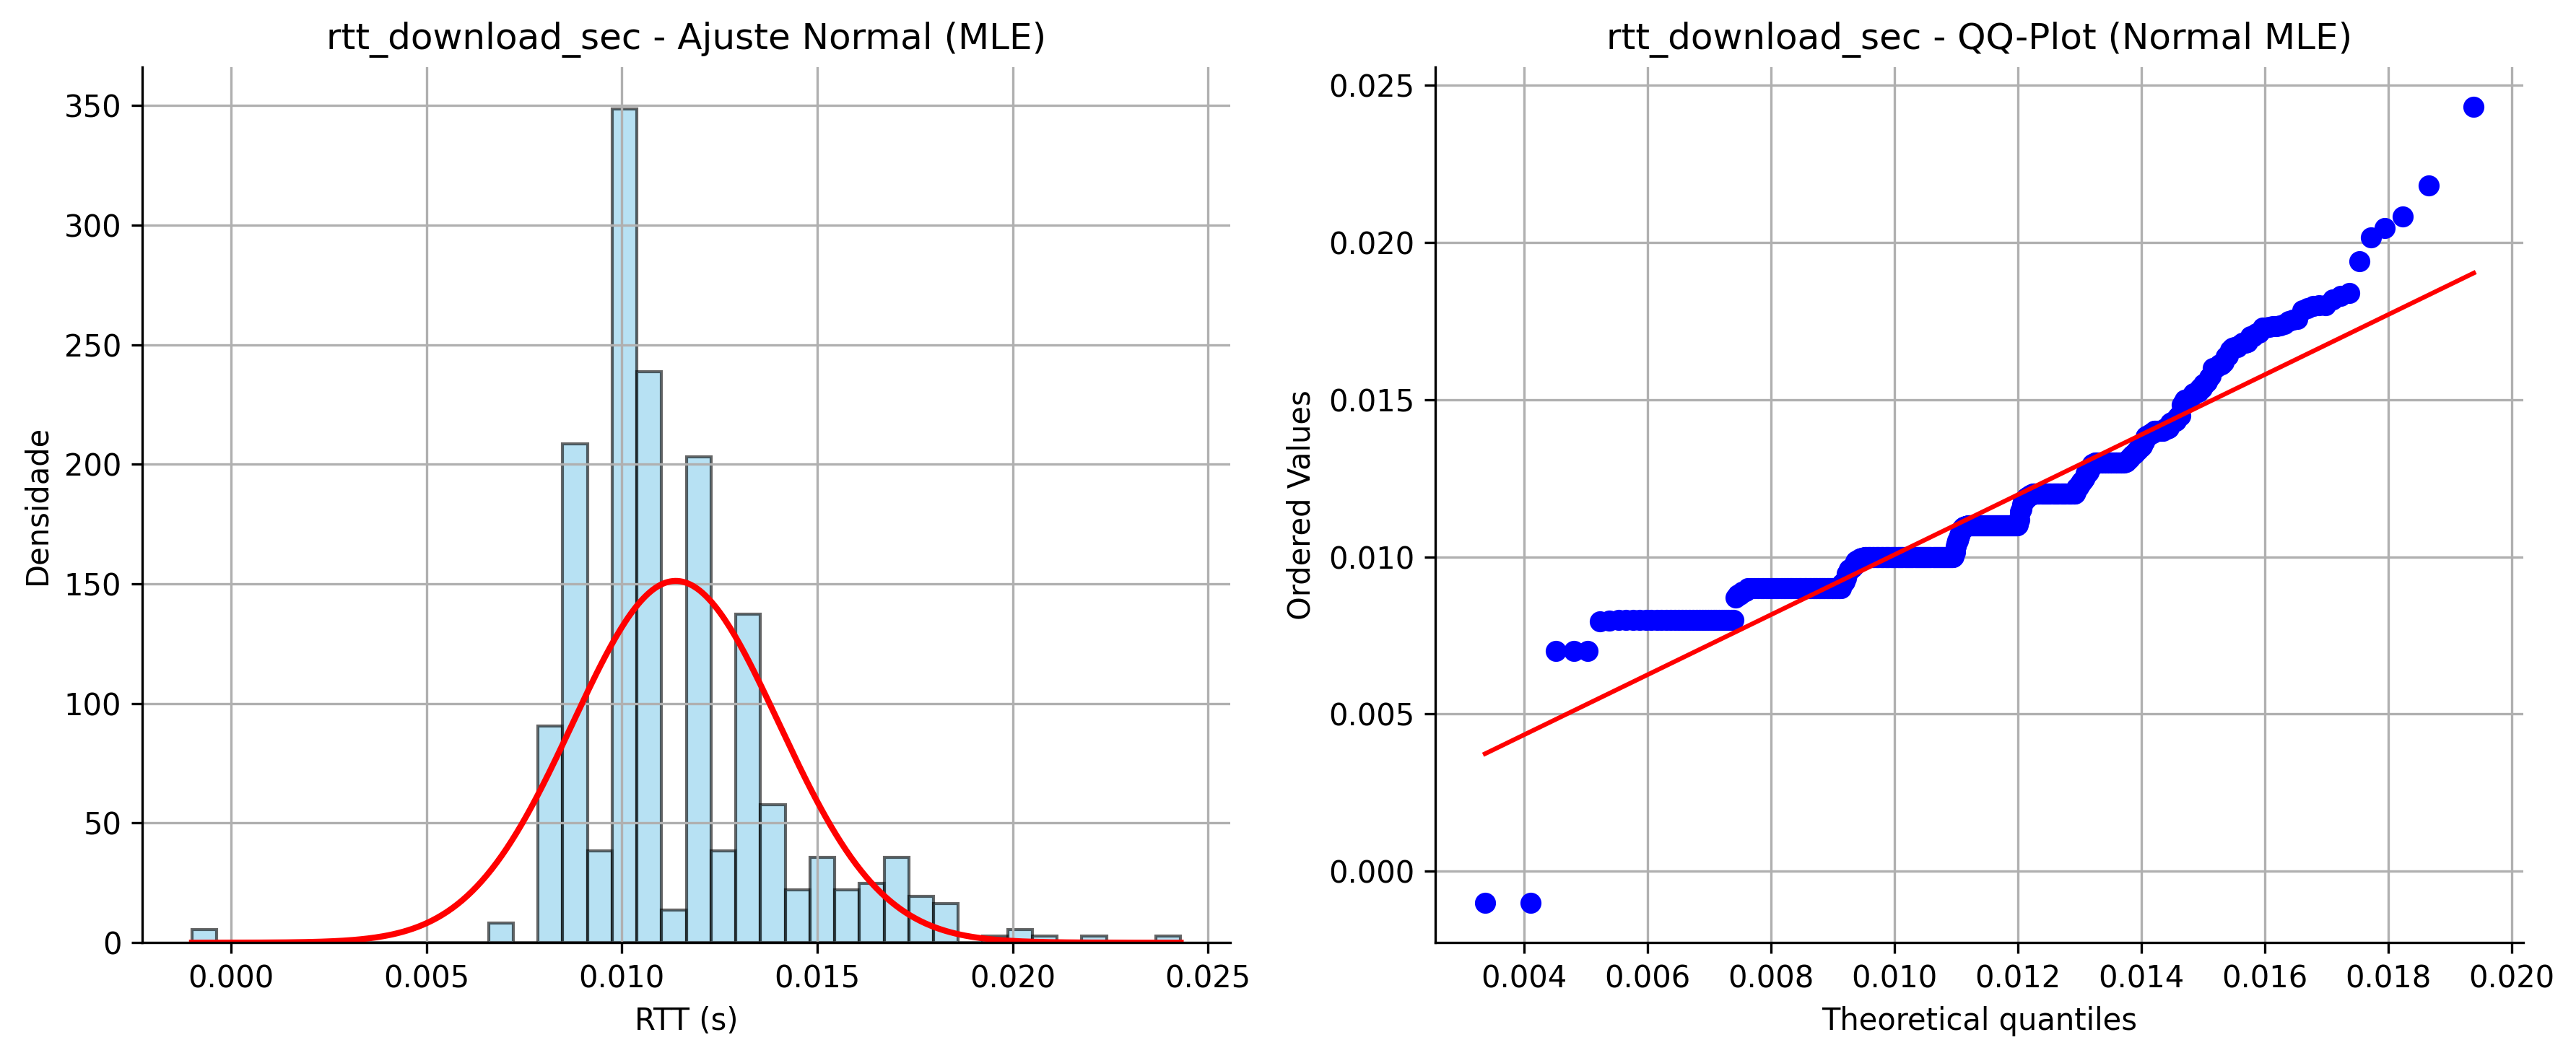
\includegraphics[width=\textwidth]{../figures/mle/rtt_download_sec_ajuste_normal_server02.png}
	\caption{Ajuste da distribuição Normal aos dados de RTT de download para o Servidor 02. O modelo se ajusta bem à forma aproximadamente simétrica da distribuição empírica.}
	\label{fig:rtt_download_sec_ajuste_normal_server02}
\end{figure}

\begin{figure}[htp]
	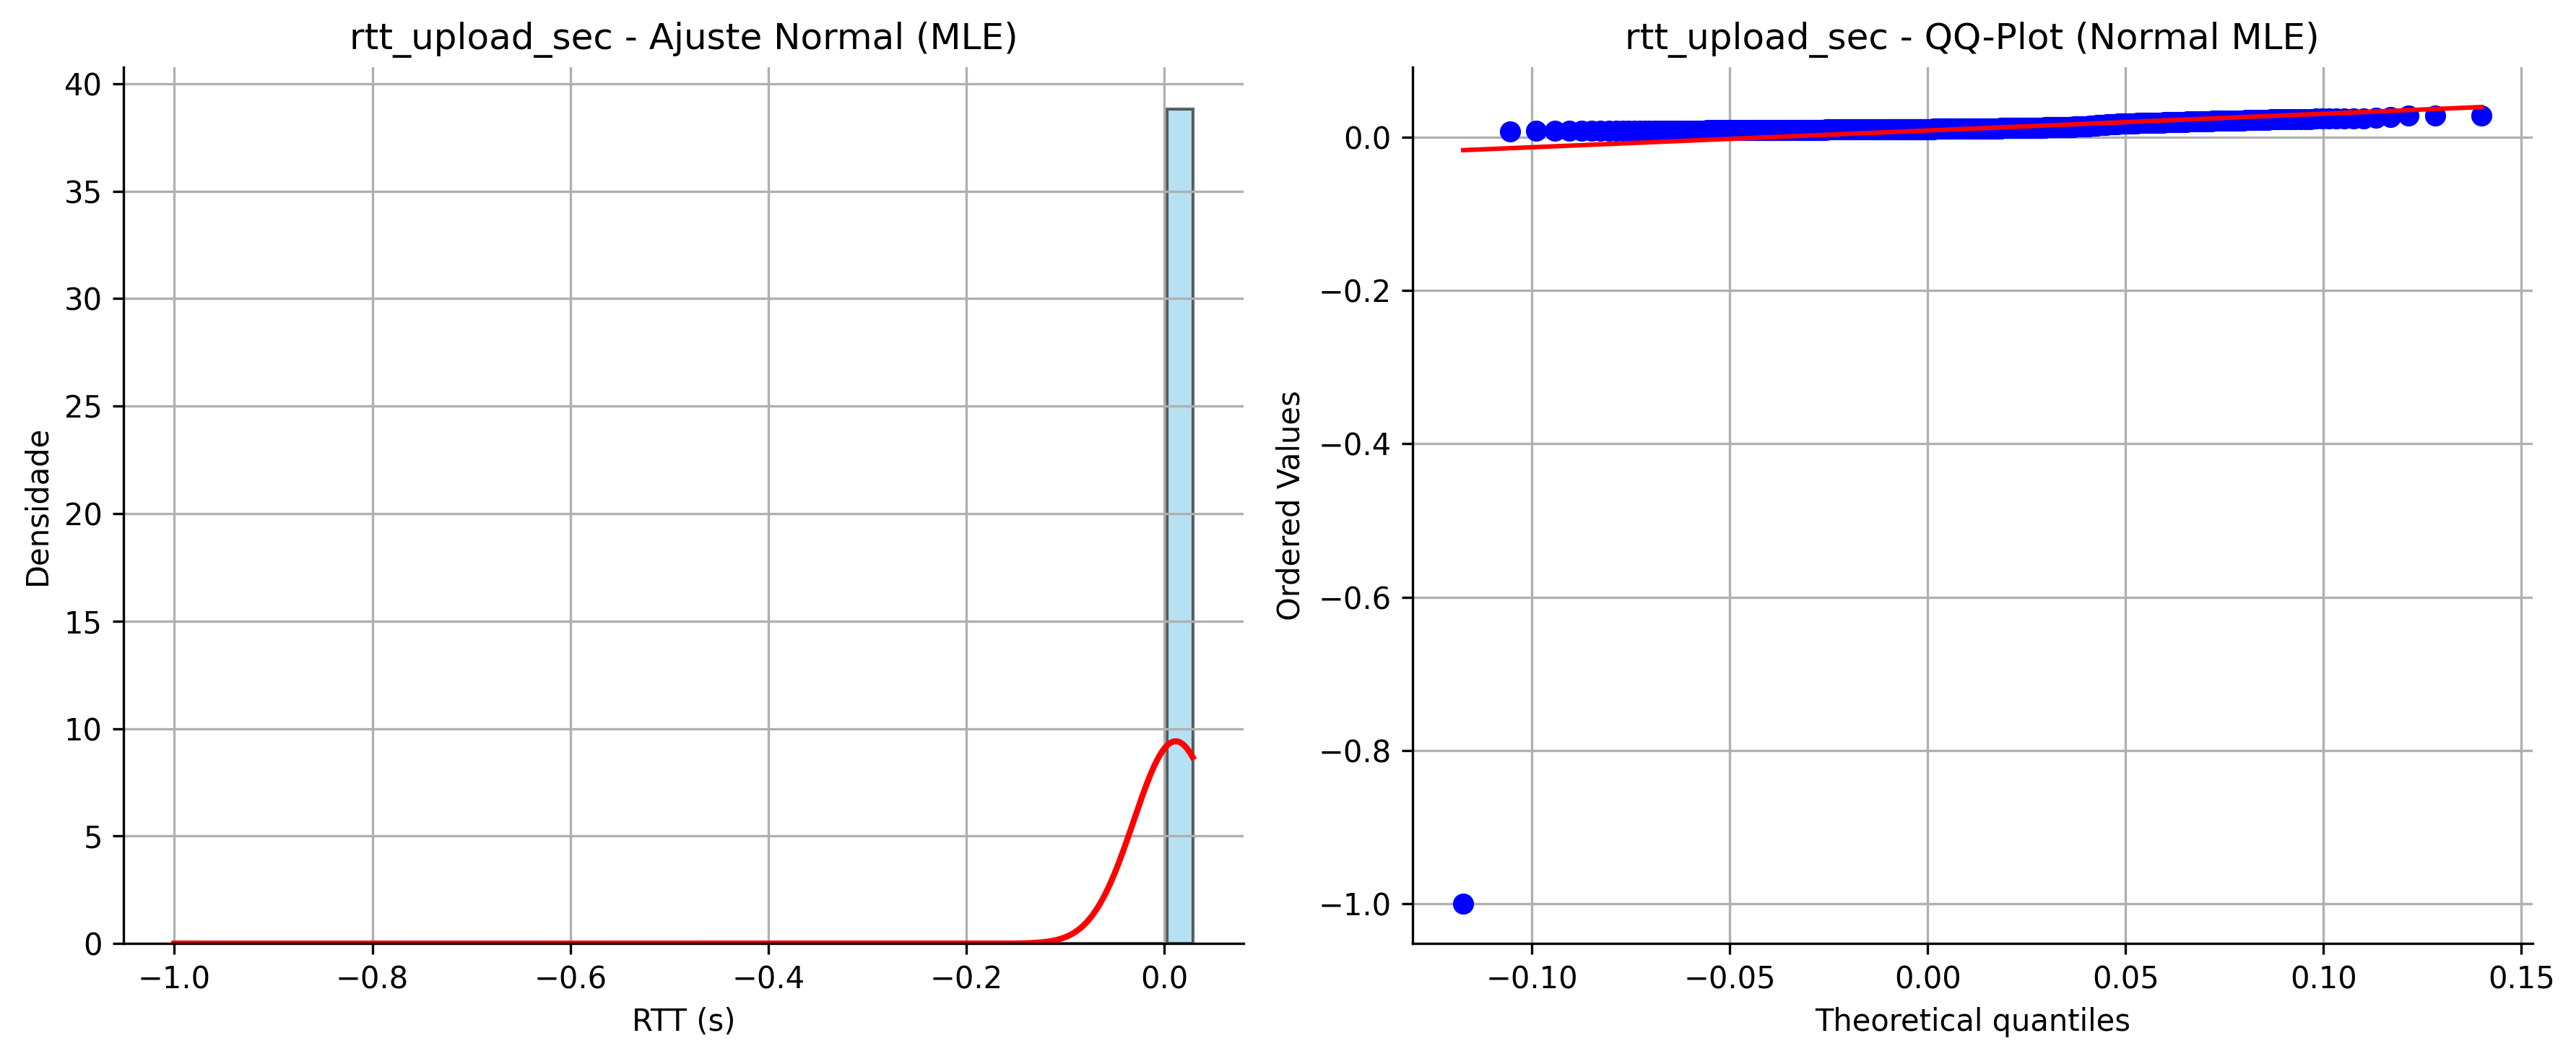
\includegraphics[width=\textwidth]{../figures/mle/rtt_upload_sec_ajuste_normal_server02.png}
	\caption{Ajuste da distribuição Normal aos dados de RTT de upload para o Servidor 02. O QQ-plot confirma a boa aderência do modelo.}
	\label{fig:rtt_upload_sec_ajuste_normal_server02}
\end{figure}

\begin{figure}[htp]
	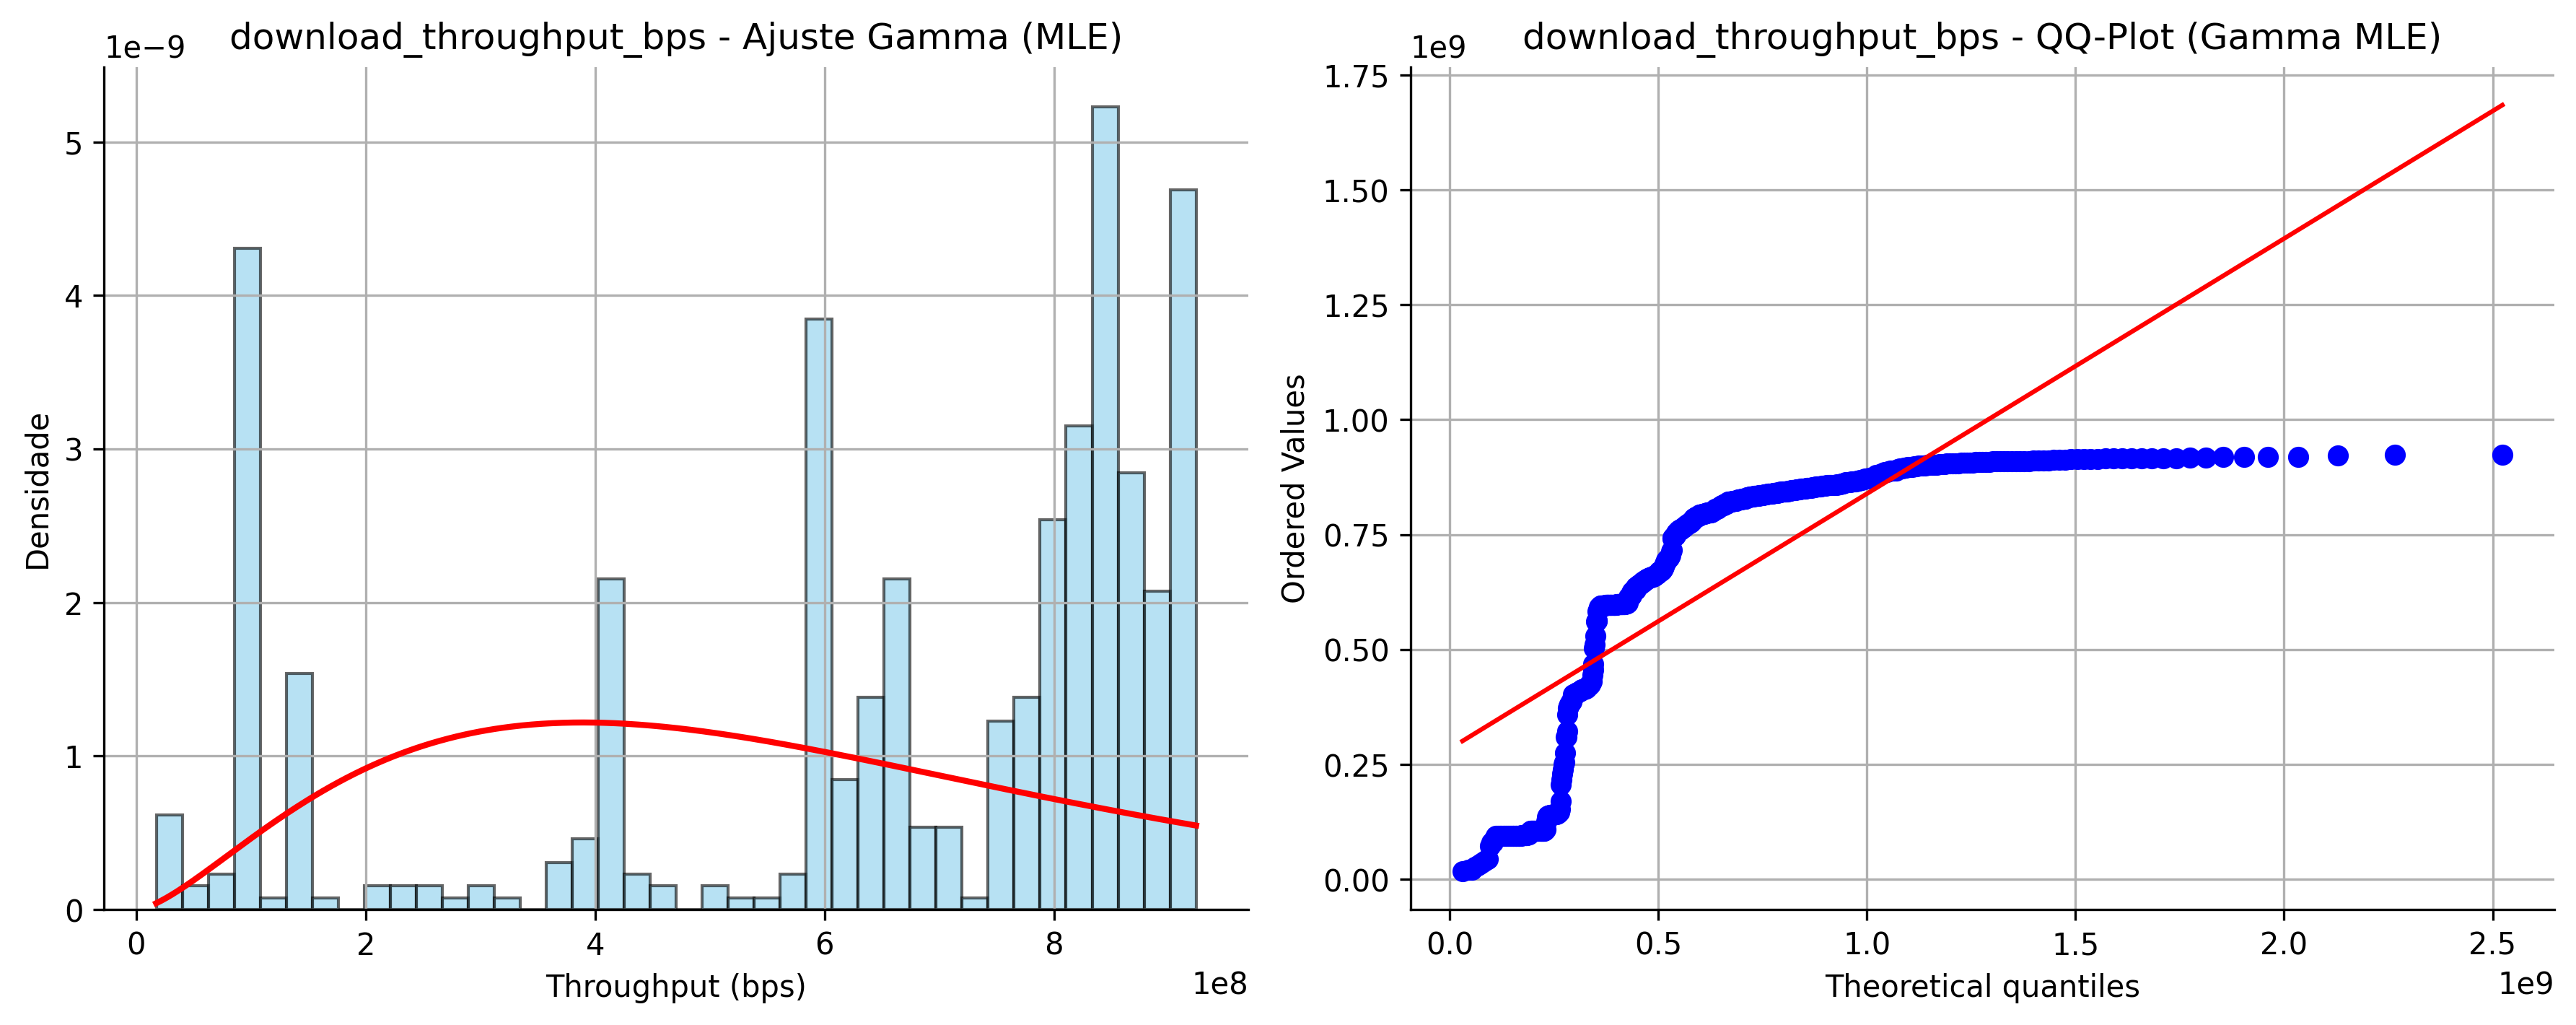
\includegraphics[width=\textwidth]{../figures/mle/download_throughput_bps_ajuste_gamma_server02.png}
	\caption{Ajuste da distribuição Gama aos dados de \textit{throughput} de download para o Servidor 02. O modelo descreve parcialmente a densidade principal, com menor precisão nas extremidades.}
	\label{fig:download_throughput_bps_ajuste_gamma_server02}
\end{figure}

\begin{figure}[htp]
	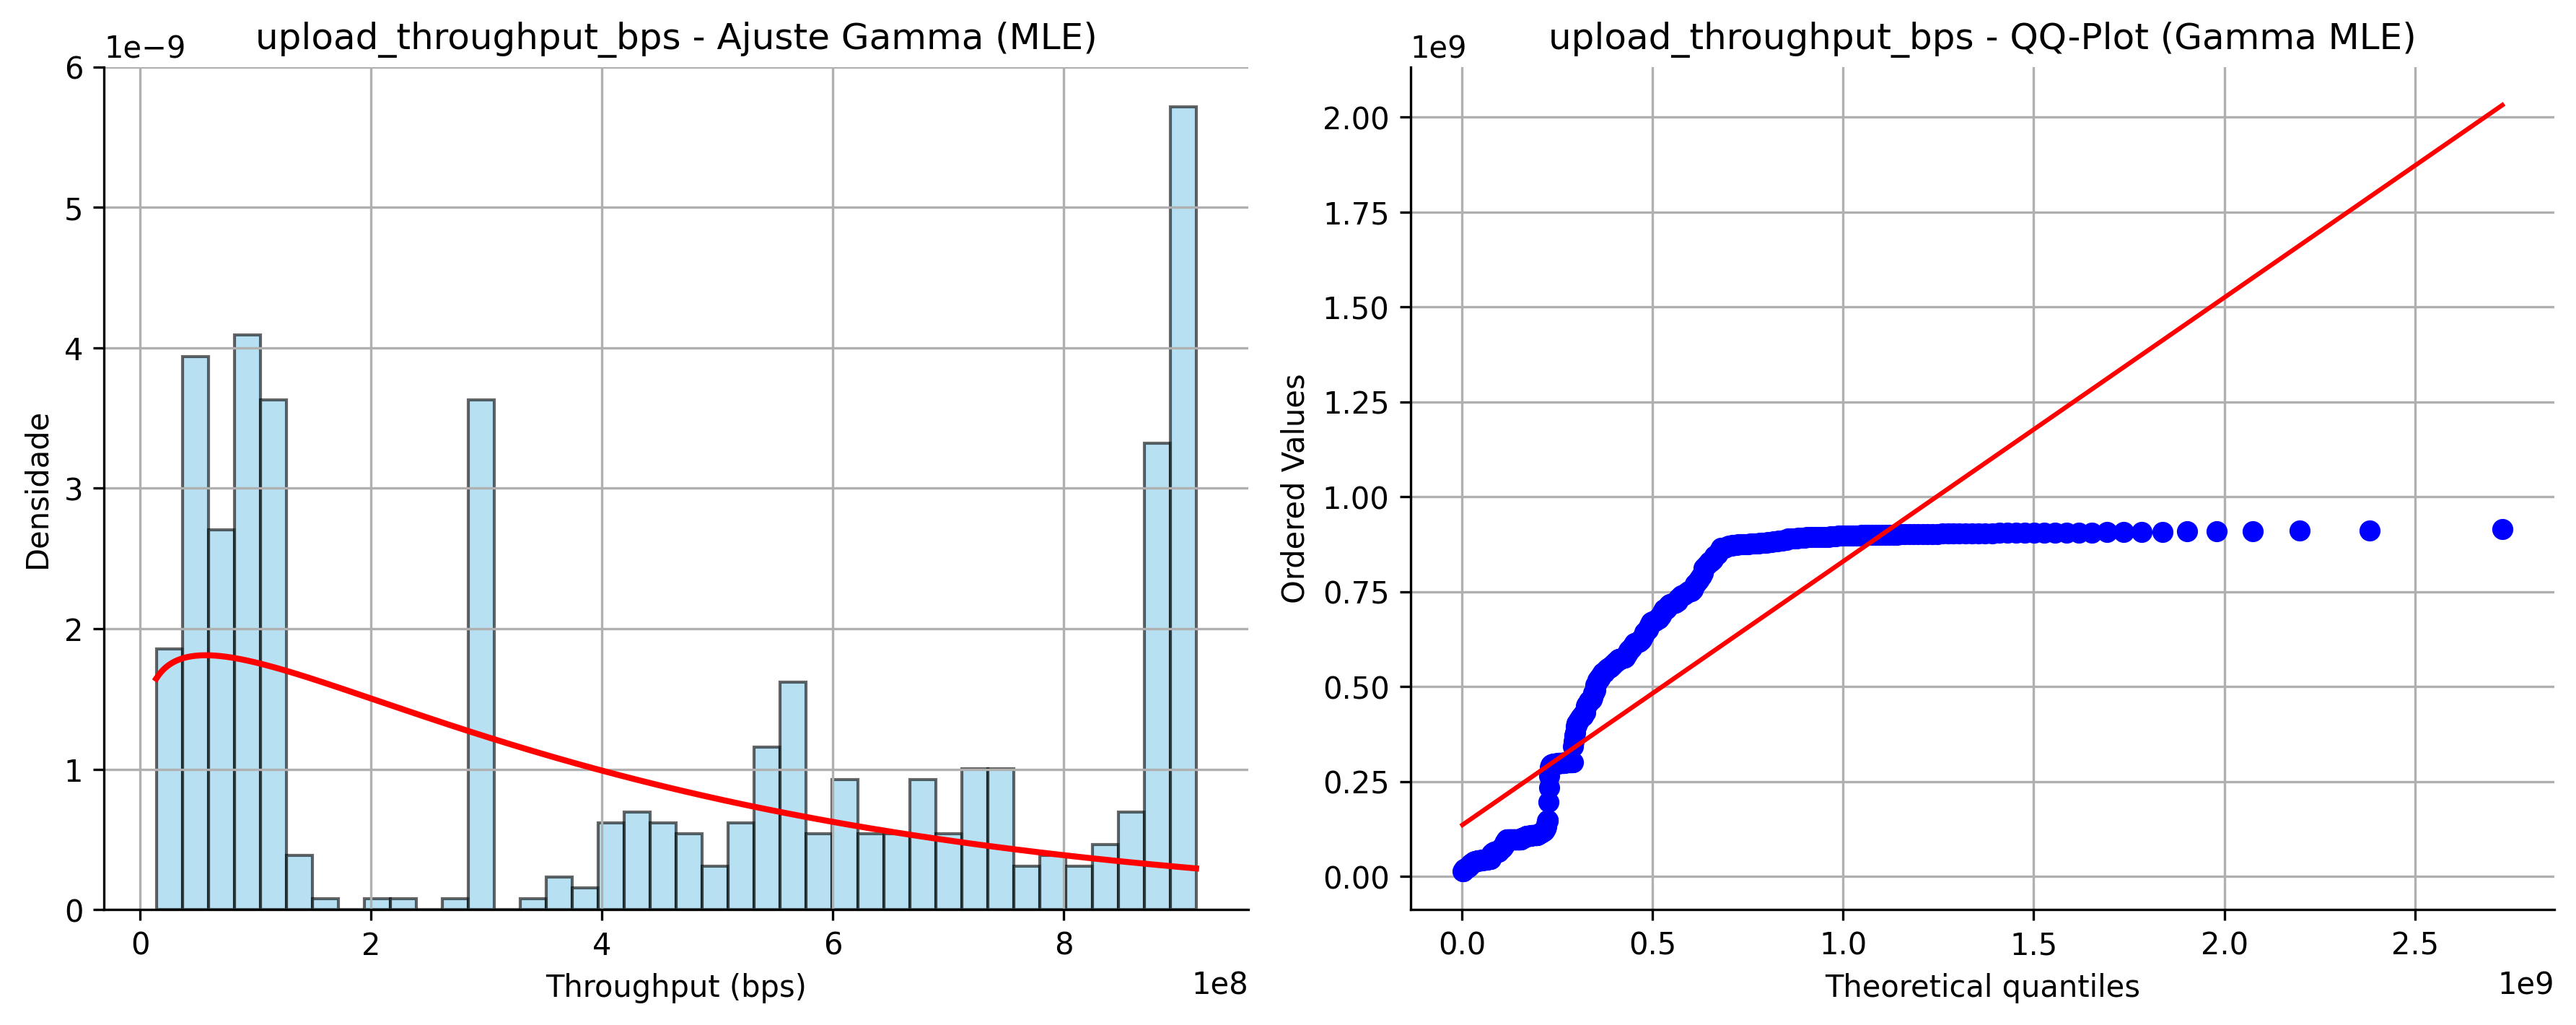
\includegraphics[width=\textwidth]{../figures/mle/upload_throughput_bps_ajuste_gamma_server02.png}
	\caption{Ajuste da distribuição Gama aos dados de \textit{throughput} de upload para o Servidor 02. Observa-se boa aproximação no centro da distribuição, mas caudas mais dispersas.}
	\label{fig:upload_throughput_bps_ajuste_gamma_server02}
\end{figure}

\begin{figure}[htp]
	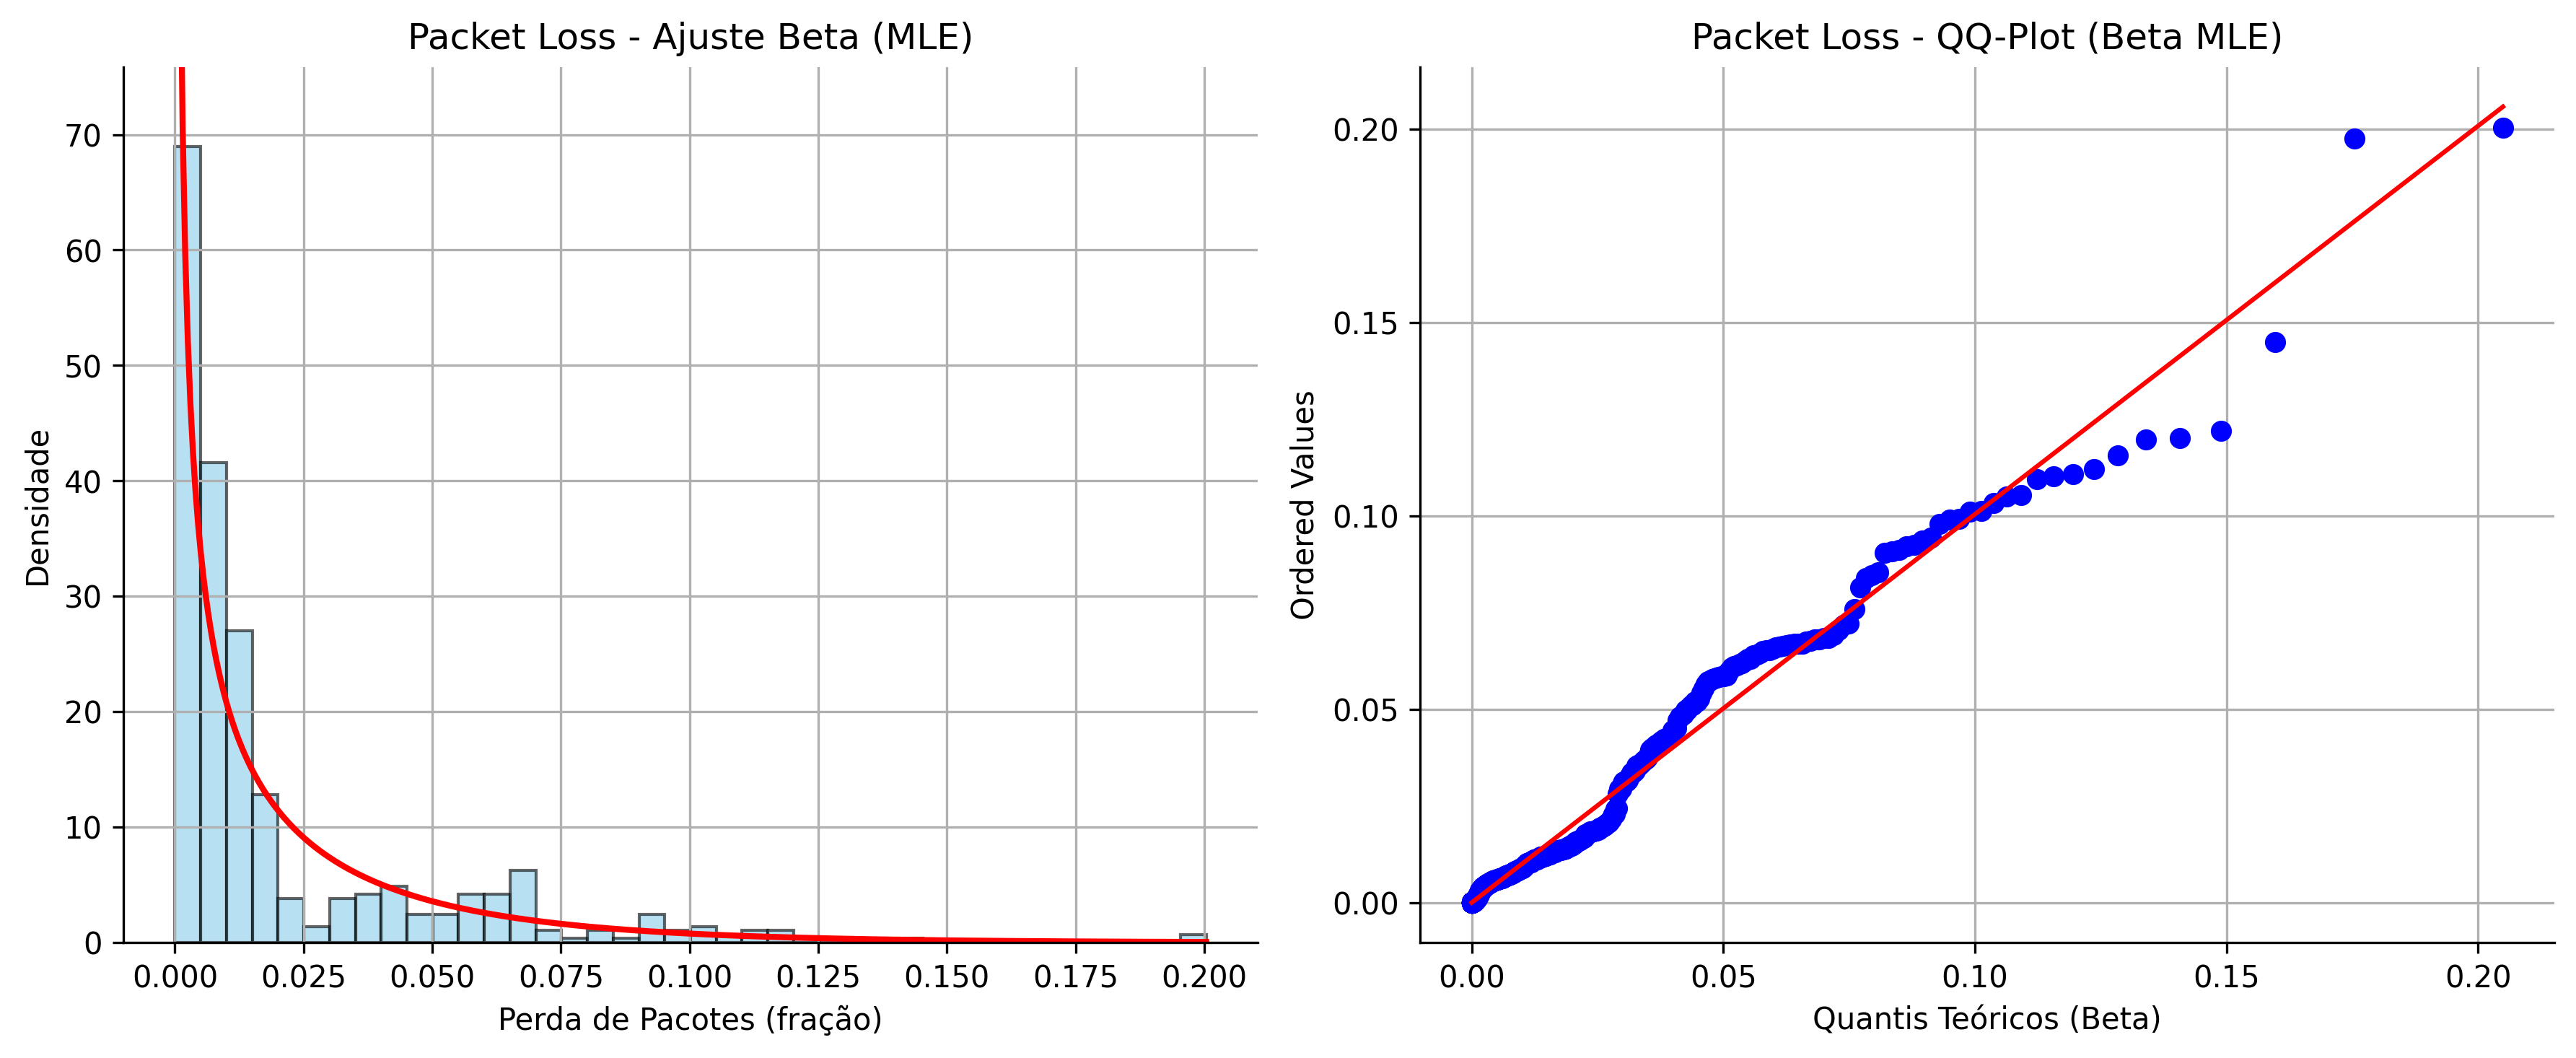
\includegraphics[width=\textwidth]{../figures/mle/packet_loss_ajuste_beta_serve02.png}
	\caption{Ajuste da distribuição Beta à variável de perda de pacotes para o Servidor 02. O modelo captura adequadamente a concentração de valores baixos e a assimetria à direita.}
	\label{fig:packet_loss_ajuste_beta_serve02}
\end{figure}

Entretanto, nas variáveis de \textit{throughput} (download e upload),
o ajuste foi ligeiramente inferior, refletindo a natureza mais irregular
da distribuição dos dados de taxa de transmissão.
Enquanto os modelos conseguem representar bem parte da massa central das observações,
eles apresentam menor capacidade de generalização nas extremidades,
provavelmente devido à grande dispersão e à presença de múltiplos regimes de transmissão
ao longo do tempo.

As superfícies de log-verossimilhança correspondentes são apresentadas nas
Figuras~\ref{fig:rtt_loglik_normal_combined_server02},
\ref{fig:throughput_gamma_loglik_combined_server02}
e \ref{fig:packet_loss_loglik_surface_beta_server02}.
Assim como no caso do cliente, essas figuras evidenciam regiões bem definidas de máximo,
indicando convergência estável do processo de estimação e ausência de múltiplos ótimos locais relevantes.

\begin{figure}[htp]
	\centering
	% Subfigure 1
	\begin{subfigure}[b]{0.48\textwidth} % Ocupa 48% da largura do texto
		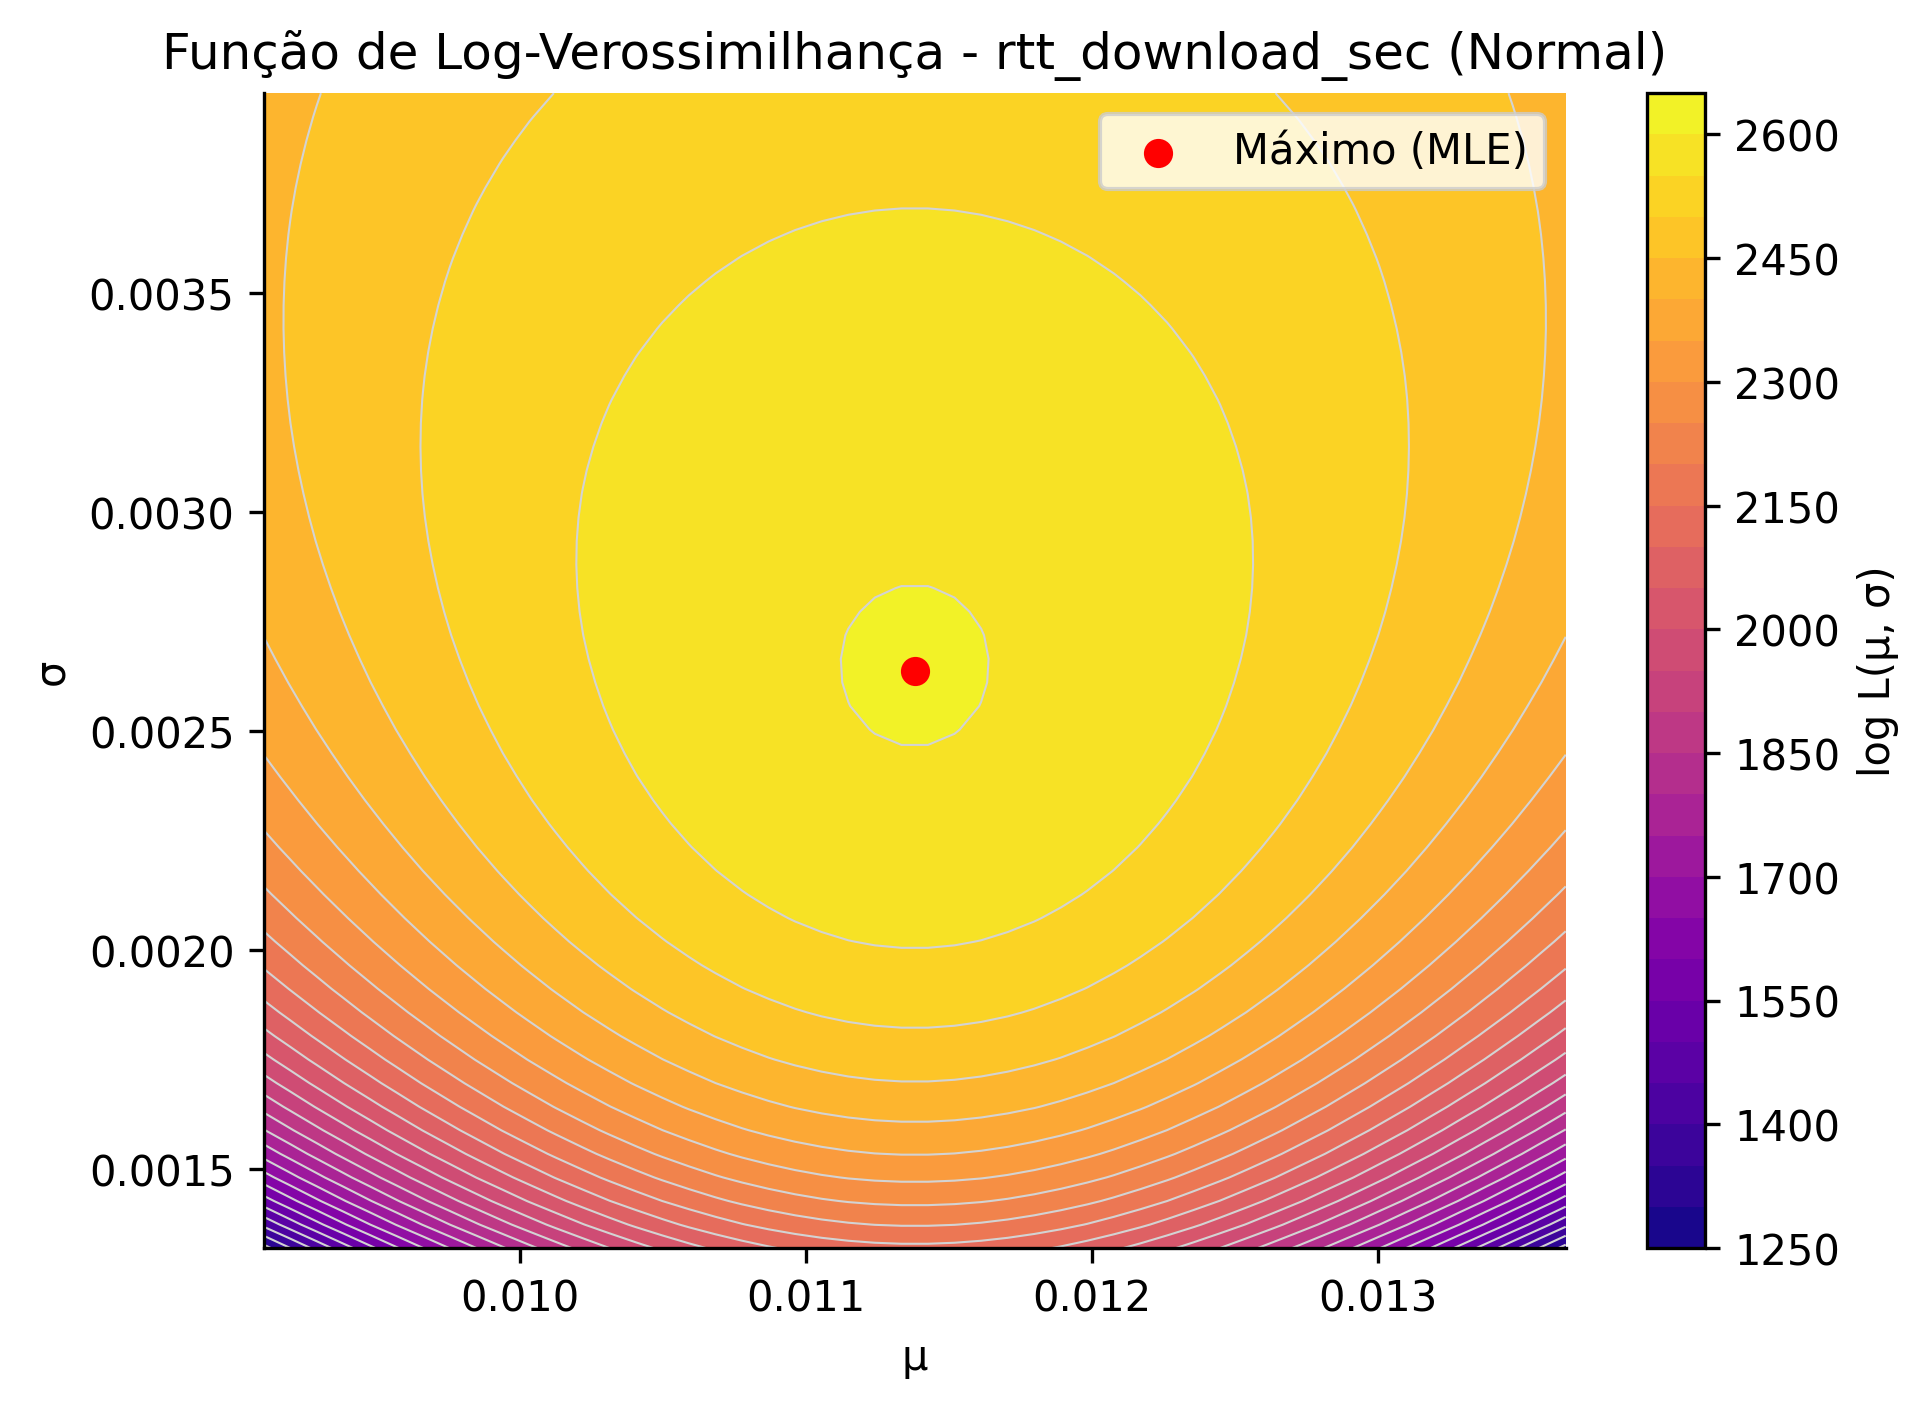
\includegraphics[width=\textwidth]{../figures/mle/rtt_download_sec_loglik_surface_normal_server02.png}
		\caption{RTT Download (Normal)}
		\label{fig:rtt_download_sec_loglik_surface_normal_server02}
	\end{subfigure}
	\hfill % Espaço horizontal entre as subfiguras
	% Subfigure 2
	\begin{subfigure}[b]{0.48\textwidth} % Ocupa 48% da largura do texto
		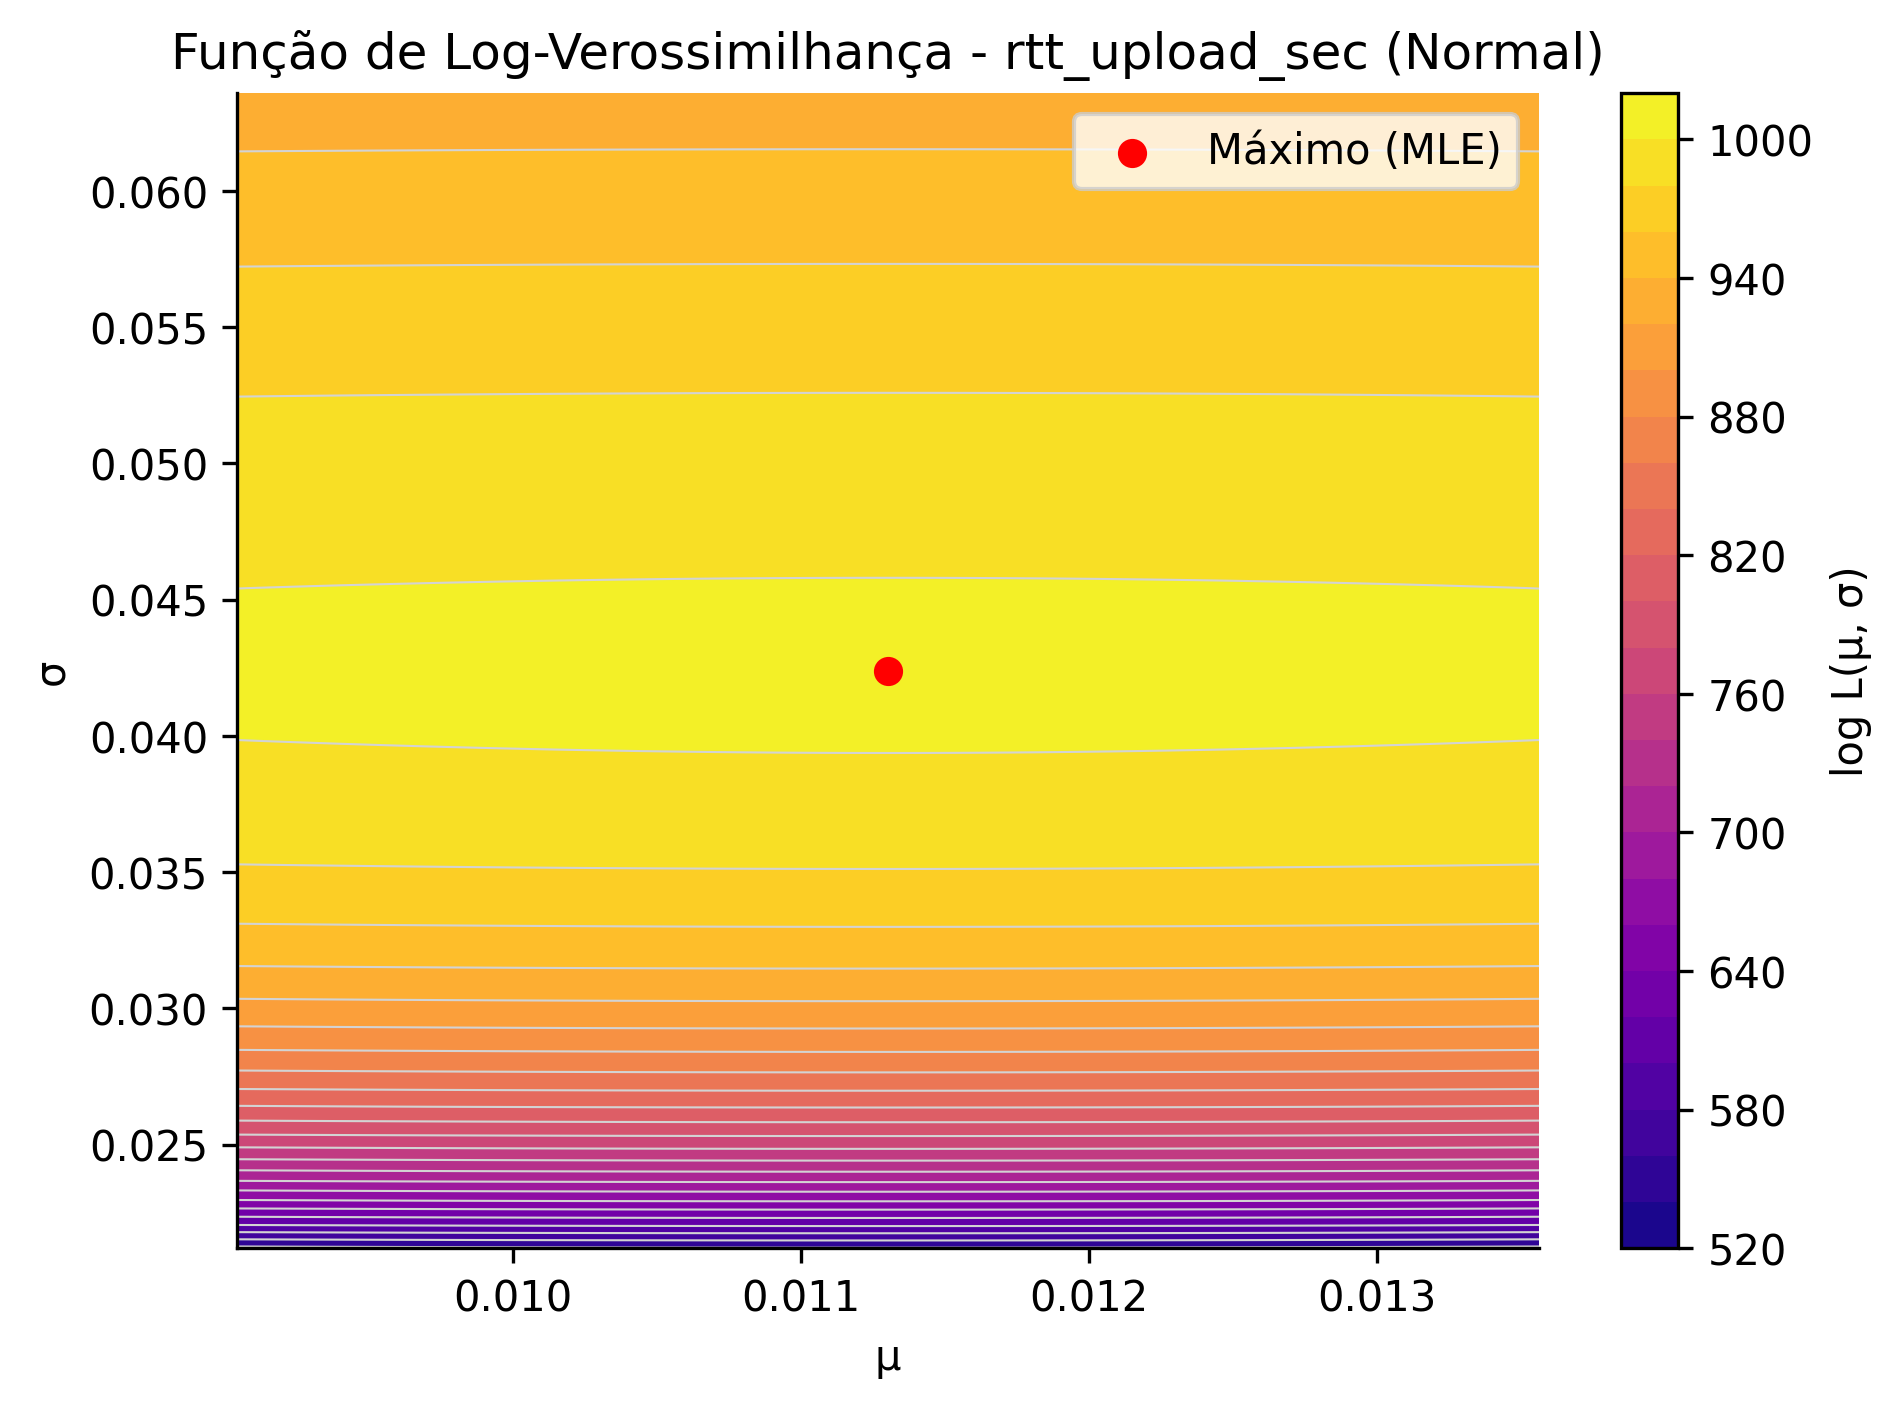
\includegraphics[width=\textwidth]{../figures/mle/rtt_upload_sec_loglik_surface_normal_server02.png}
		\caption{RTT Upload (Normal)}
		\label{fig:rtt_upload_sec_loglik_surface_normal_server02}
	\end{subfigure}
	\caption{Superfícies de log-verossimilhança para os parâmetros $\mu$ e $\sigma$ da distribuição Normal (RTT) ajustada ao Servidor 02.}
	\label{fig:rtt_loglik_normal_combined_server02}
\end{figure}

\begin{figure}[htp]
	\centering
	\begin{subfigure}[b]{0.48\textwidth} % Ocupa 48% da largura do texto
		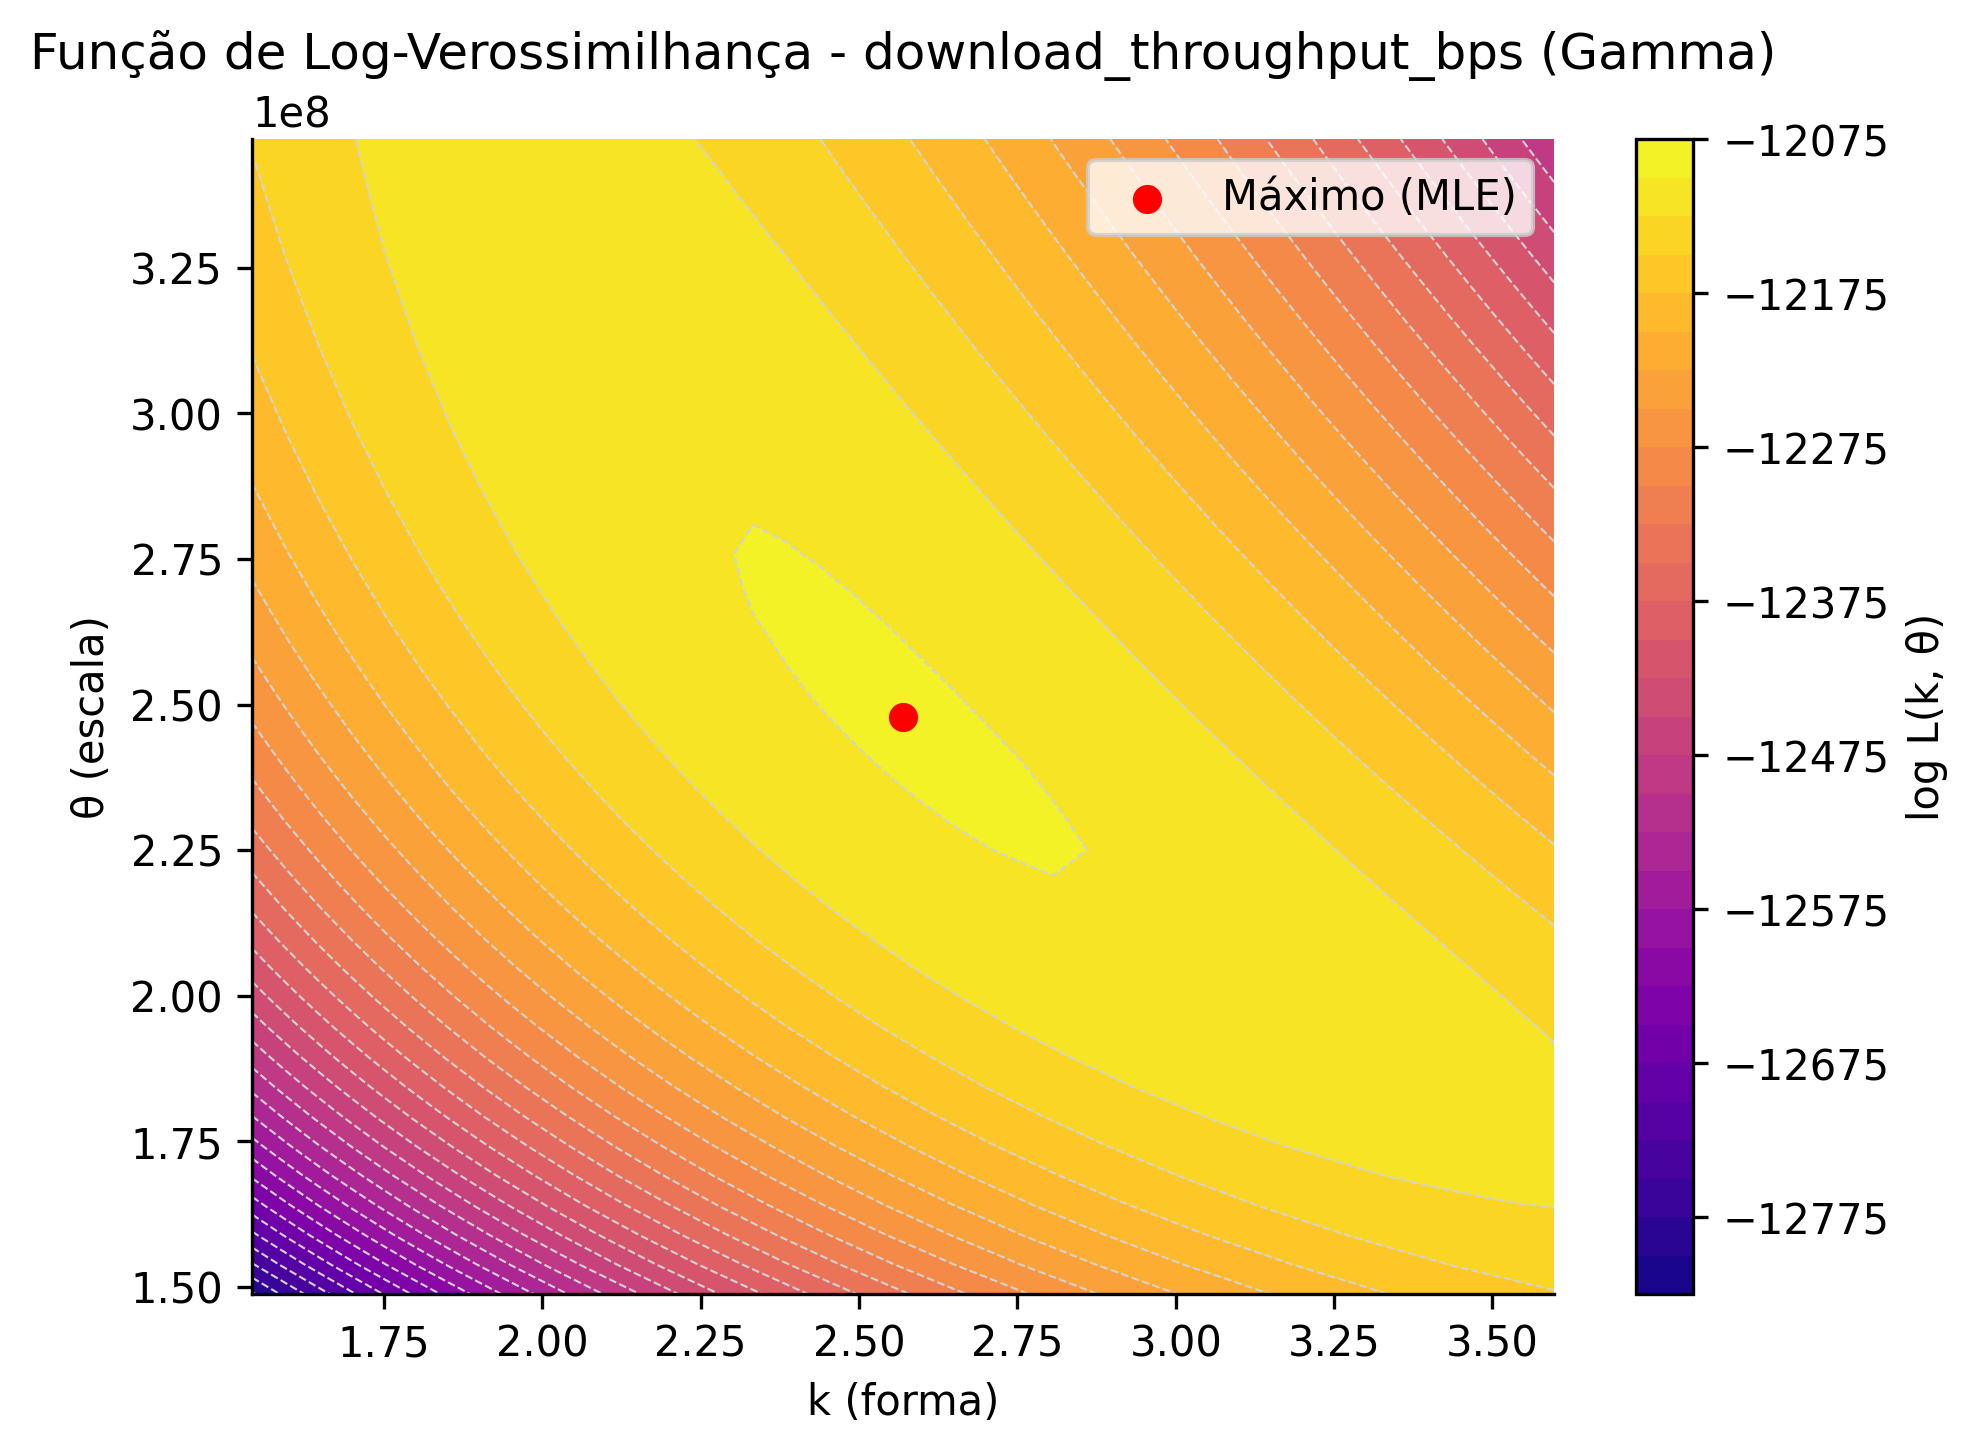
\includegraphics[width=\textwidth]{../figures/mle/download_throughput_bps_loglik_surface_gamma_server02.png}
		\caption{Throughput de Download (Distribuição Gamma)}
		\label{fig:download_throughput_bps_loglik_surface_gamma_server02}
	\end{subfigure}
	\hfill 
	\begin{subfigure}[b]{0.48\textwidth}
		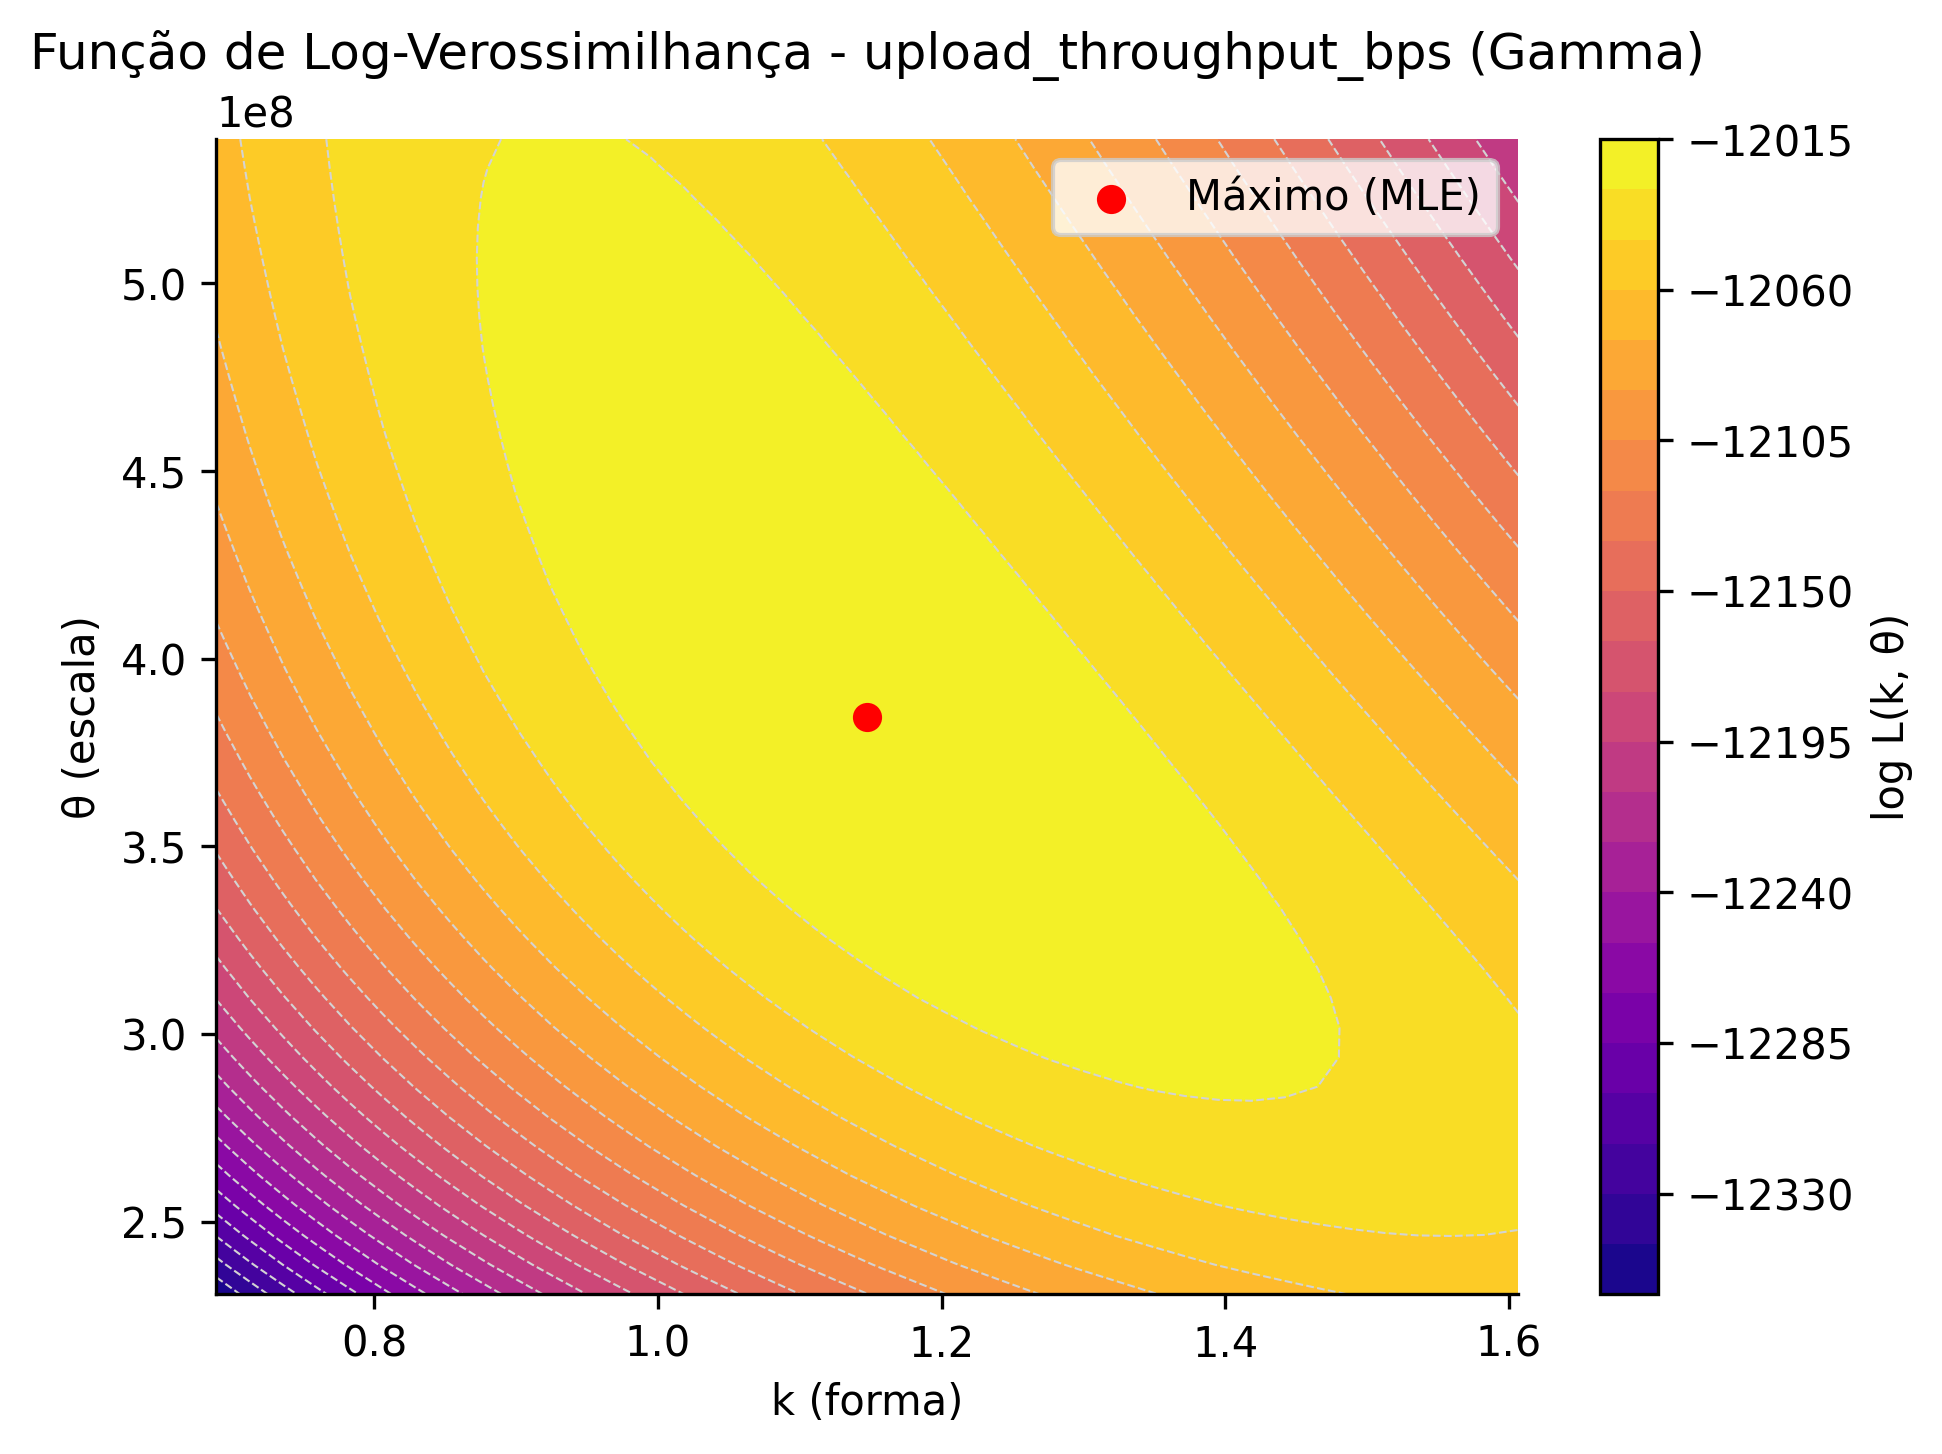
\includegraphics[width=\textwidth]{../figures/mle/upload_throughput_bps_loglik_surface_gamma_server02.png}
		\caption{Throughput de Upload (Distribuição Gamma)}
		\label{fig:upload_throughput_bps_loglik_surface_gamma_server02}
	\end{subfigure}
	\caption{Superfícies de log-verossimilhança para os parâmetros $k$ e $\theta$ da distribuição Gama aplicada às variáveis de \textit{throughput} do Servidor 02.}
	\label{fig:throughput_gamma_loglik_combined_server02}
\end{figure}

\begin{figure}[htp]
	\centering
	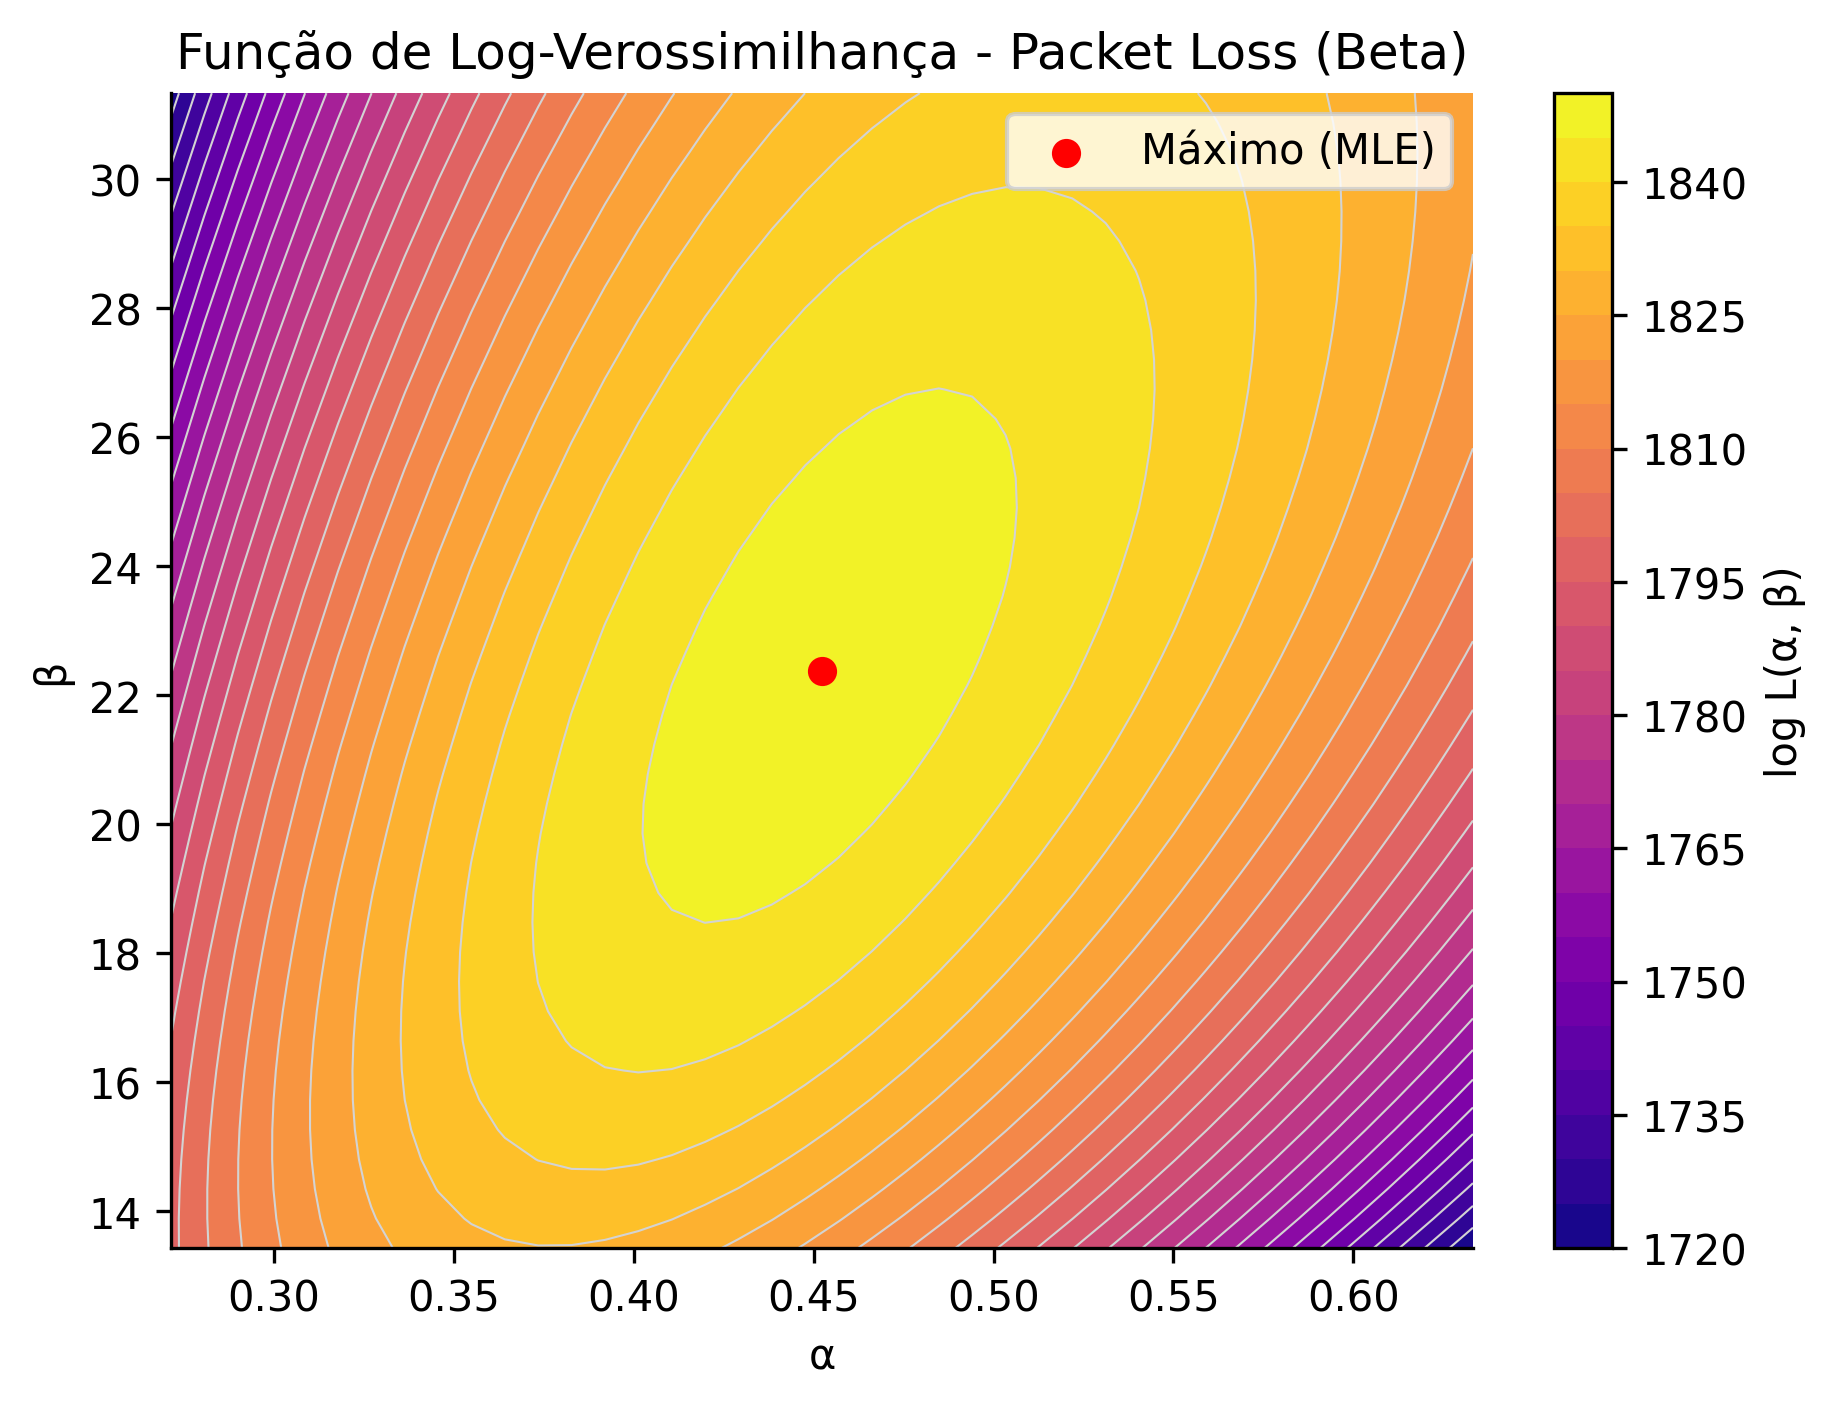
\includegraphics[width=0.48\textwidth]{../figures/mle/packet_loss_loglik_surface_beta_server02.png}
	\caption{Superfície de log-verossimilhança para os parâmetros $\alpha$ e $\beta$ da distribuição Beta ajustada à variável de perda de pacotes do Servidor 02.}
	\label{fig:packet_loss_loglik_surface_beta_server02}
\end{figure}

Os valores finais estimados para o Servidor 02 estão resumidos na
Tabela~\ref{tab:mle_parameters_server02},
correspondendo aos parâmetros que maximizam a verossimilhança para cada modelo ajustado.

\begin{table}[htp]
	\centering
	\caption{Parâmetros estimados por Máxima Verossimilhança (MLE) para o Servidor 02. Os valores representam os pares de parâmetros que maximizam a log-verossimilhança de cada modelo ajustado.}
	\label{tab:mle_parameters_server02}
	\begin{tabular}{|l|c|l|}
		\hline
		\textbf{Variável} & \textbf{Distribuição} & \textbf{Parâmetros MLE} \\
		\hline
		rtt\_download\_sec & Normal & $\hat{\mu}=0.01138$, $\hat{\sigma}=0.002638$ \\
		\hline
		rtt\_upload\_sec & Normal & $\hat{\mu}=0.0113$, $\hat{\sigma}=0.04239$ \\
		\hline
		download\_throughput\_bps & Gamma & $\hat{k}=2.57$, $\hat{\theta}=2.479 \times 10^8$ \\
		\hline
		upload\_throughput\_bps & Gamma & $\hat{k}=1.148$, $\hat{\theta}=3.846 \times 10^8$ \\
		\hline
		packet\_loss\_percent & Beta & $\hat{\alpha}=0.4523$, $\hat{\beta}=22.38$ \\
		\hline
	\end{tabular}
\end{table}

De modo geral, os resultados obtidos por MLE confirmam a adequação dos modelos propostos
e indicam que as distribuições Normal, Gama e Beta foram capazes de capturar satisfatoriamente
o comportamento estatístico das variáveis de desempenho de rede analisadas.
Esses parâmetros servirão de base para as próximas análises de Inferência Bayesiana,
nas quais serão incorporadas informações \textit{a priori} e avaliadas as incertezas associadas
aos modelos ajustados.

\subsection{Inferência Bayesiana}

A inferência Bayesiana oferece uma abordagem probabilística para a estimação de parâmetros,
permitindo incorporar incertezas prévias sobre o modelo e atualizar essas crenças à medida
que novos dados são observados. Diferentemente do método de Máxima Verossimilhança (MLE),
que busca um ponto ótimo para o parâmetro $\hat{\theta}_{MLE}$, a inferência Bayesiana
calcula a distribuição completa dos parâmetros condicionada aos dados, expressa por:
\begin{equation}
	p(\theta | x) = \frac{p(x | \theta) \, p(\theta)}{p(x)},
\end{equation}
onde $p(\theta)$ é a distribuição \textit{a priori}, $p(x|\theta)$ é a função de
verossimilhança e $p(\theta|x)$ é a \textit{a posteriori}, que resume o conhecimento atualizado
sobre os parâmetros após observar os dados.

\subsubsection{Especificação das Priors e Modelos Utilizados}

Para cada variável, foi adotado um modelo probabilístico coerente com sua natureza estatística,
mantendo a mesma escolha empregada na etapa de MLE:
\begin{itemize}
	\item \textbf{RTT (Download e Upload):} modelo \textbf{Normal–Normal}, assumindo variância
	conhecida e inferência apenas sobre a média $\mu$;
	\item \textbf{Throughput (Download e Upload):} modelo \textbf{Gamma–Gamma}, adequado para
	variáveis contínuas positivas e assimétricas;
	\item \textbf{Perda de Pacotes:} modelo \textbf{Beta–Binomial}, apropriado para proporções
	limitadas ao intervalo $[0, 1]$.
\end{itemize}

As distribuições \textit{a priori} foram escolhidas de forma \textbf{fracamente informativa},
permitindo que os dados observados tivessem maior influência no processo de atualização.
Essa decisão foi importante devido à natureza empírica dos dados, cuja variabilidade é ampla
e de difícil parametrização prévia.

\subsubsection{Cálculo dos Parâmetros Posteriores}

Para o modelo Normal–Normal adotado no RTT, considerando $\sigma^2$ conhecida, a posterior
resulta também em uma distribuição Normal:
\begin{equation}
	\mu | x \sim \mathcal{N}(\mu_n, \sigma_n^2),
\end{equation}
onde os parâmetros atualizados são dados por:
\begin{equation}
	\sigma_n^2 = \left( \frac{1}{\sigma_0^2} + \frac{n}{\sigma^2} \right)^{-1},
	\qquad
	\mu_n = \sigma_n^2 \left( \frac{\mu_0}{\sigma_0^2} + \frac{n \bar{x}}{\sigma^2} \right).
\end{equation}

A distribuição \textbf{preditiva posterior} é obtida pela integração dos parâmetros e segue
uma Normal:
\begin{equation}
	p(x_{new}|x) = \mathcal{N}(\mu_n, \sigma^2 + \sigma_n^2),
\end{equation}
cujo valor esperado e variância são, respectivamente:
\[
E[x_{new}|x] = \mu_n, \qquad
Var[x_{new}|x] = \sigma^2 + \sigma_n^2.
\]

Para as variáveis com modelos Gama–Gama e Beta–Binomial, os parâmetros de forma e taxa
foram atualizados de modo análogo, resultando em posteriors da mesma família que suas priors,
mantendo a conjugação e simplificando o cálculo das distribuições preditivas.

\subsubsection{Resultados para o Cliente 13}

As Figuras~\ref{fig:rtt_download_sec_bayesian_normalnormal_client13}
e~\ref{fig:rtt_upload_sec_bayesian_normalnormal_client13} apresentam as distribuições
a priori, a posteriori e preditiva para o \textit{RTT} de \textit{download} e \textit{upload}.
Em ambos os casos, observa-se que a atualização bayesiana convergiu fortemente em torno da média
observada, refletindo alta consistência entre as informações prévias e os dados empíricos.
As curvas preditivas (em preto) se sobrepõem de forma satisfatória à distribuição dos dados de teste,
indicando excelente desempenho do modelo.

\begin{figure}[htp]
	\centering
	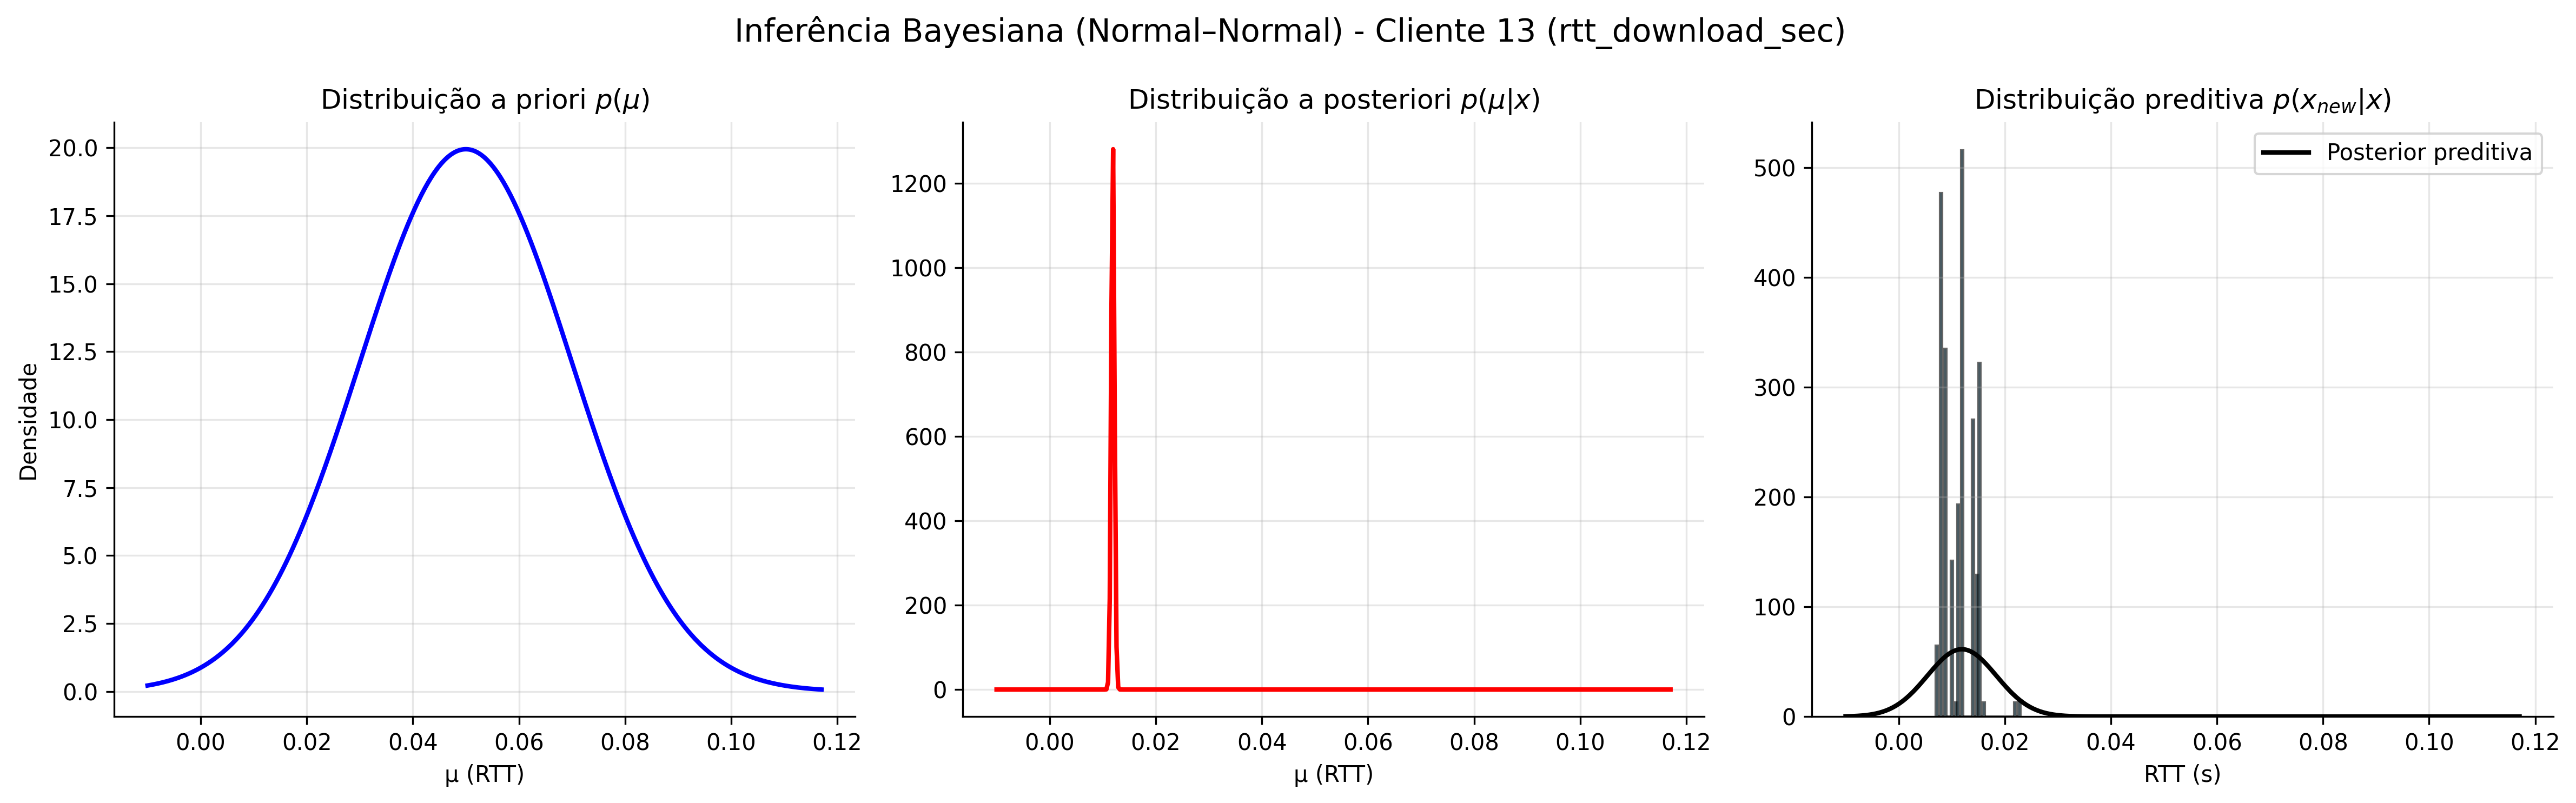
\includegraphics[width=\textwidth]{../figures/bayes/rtt_download_sec_bayesian_normalnormal_client13.png}
	\caption{.}
	\label{fig:rtt_download_sec_bayesian_normalnormal_client13}
\end{figure}
\begin{figure}[htp]
	\centering
	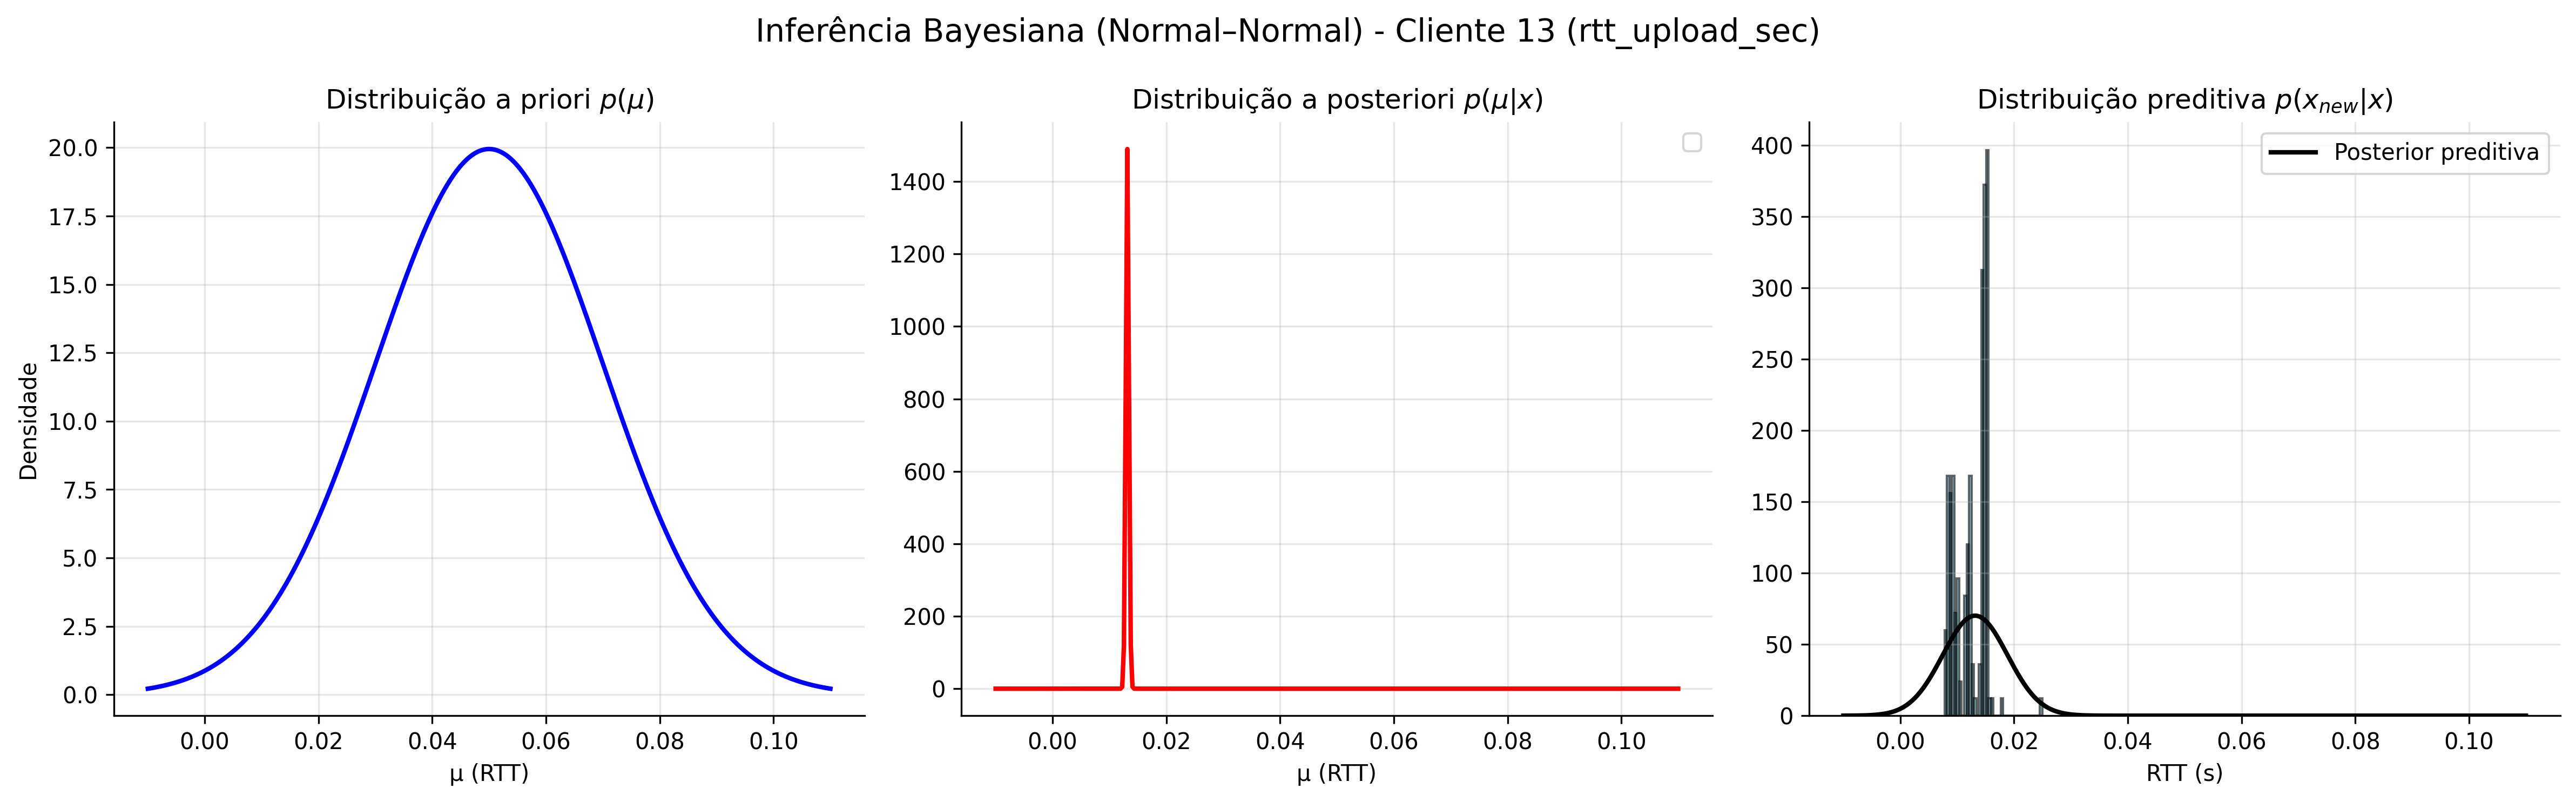
\includegraphics[width=\textwidth]{../figures/bayes/rtt_upload_sec_bayesian_normalnormal_client13.png}
	\caption{.}
	\label{fig:rtt_upload_sec_bayesian_normalnormal_client13}
\end{figure}

\begin{table}[htp]
	\centering
	\caption{Comparação entre prior e posterior para o Cliente 13 — RTT Download.}
	\label{tab:bayes_rtt_download_client13}
	\begin{tabular}{lcc}
		\hline
		\textbf{Parâmetro} & \textbf{Prior} & \textbf{Posterior} \\ \hline
		$\mu$ & 0.050000 & 0.011913 \\
		$\sigma^2_{\mu}$ & 0.000400 & 9.38e-08 \\
		$\sigma$ (Assumido) & -- & 0.006499 \\ \hline
	\end{tabular}
\end{table}

\begin{table}[htp]
	\centering
	\caption{Comparação entre prior e posterior para o Cliente 13 — RTT Upload.}
	\label{tab:bayes_rtt_upload_client13}
	\begin{tabular}{lcc}
		\hline
		\textbf{Parâmetro} & \textbf{Prior} & \textbf{Posterior} \\ \hline
		$\mu$ & 0.050000 & 0.013159 \\
		$\sigma^2_{\mu}$ & 0.000400 & 7.17e-08 \\
		$\sigma$ (Assumido) & -- & 0.005682 \\ \hline
	\end{tabular}
\end{table}

O mesmo comportamento foi verificado para as variáveis de \textit{Throughput}
(Download e Upload), cujos resultados estão ilustrados nas
Figuras~\ref{fig:download_throughput_bps_bayesian_gammagamma_client13}
e~\ref{fig:upload_throughput_bps_bayesian_gammagamma_client13}.
Ambas apresentaram convergência rápida e previsões com médias próximas às obtidas via MLE,
como mostrado nas tabelas a seguir:

\begin{table}[htp]
	\centering
	\caption{Convergência dos parâmetros (Gamma–Gamma) — Cliente 13 (Download).}
	\label{tab:bayes_gamma_download_client13}
	\begin{tabular}{lcc}
		\hline
		\textbf{Parâmetro} & \textbf{Prior} & \textbf{Posterior} \\ \hline
		$E[\beta]$ (Média da Taxa) & 1.00e+06 & 0.0000 \\
		$Var[\beta]$ (Variância da Taxa) & 1.00e+12 & 0.0000 \\ \hline
	\end{tabular}
\end{table}

\begin{table}[htp]
	\centering
	\caption{Convergência dos parâmetros (Gamma–Gamma) — Cliente 13 (Upload).}
	\label{tab:bayes_gamma_upload_client13}
	\begin{tabular}{lcc}
		\hline
		\textbf{Parâmetro} & \textbf{Prior} & \textbf{Posterior} \\ \hline
		$E[\beta]$ (Média da Taxa) & 1.00e+06 & 0.0000 \\
		$Var[\beta]$ (Variância da Taxa) & 1.00e+12 & 0.0000 \\ \hline
	\end{tabular}
\end{table}

\begin{figure}[htp]
	\centering
	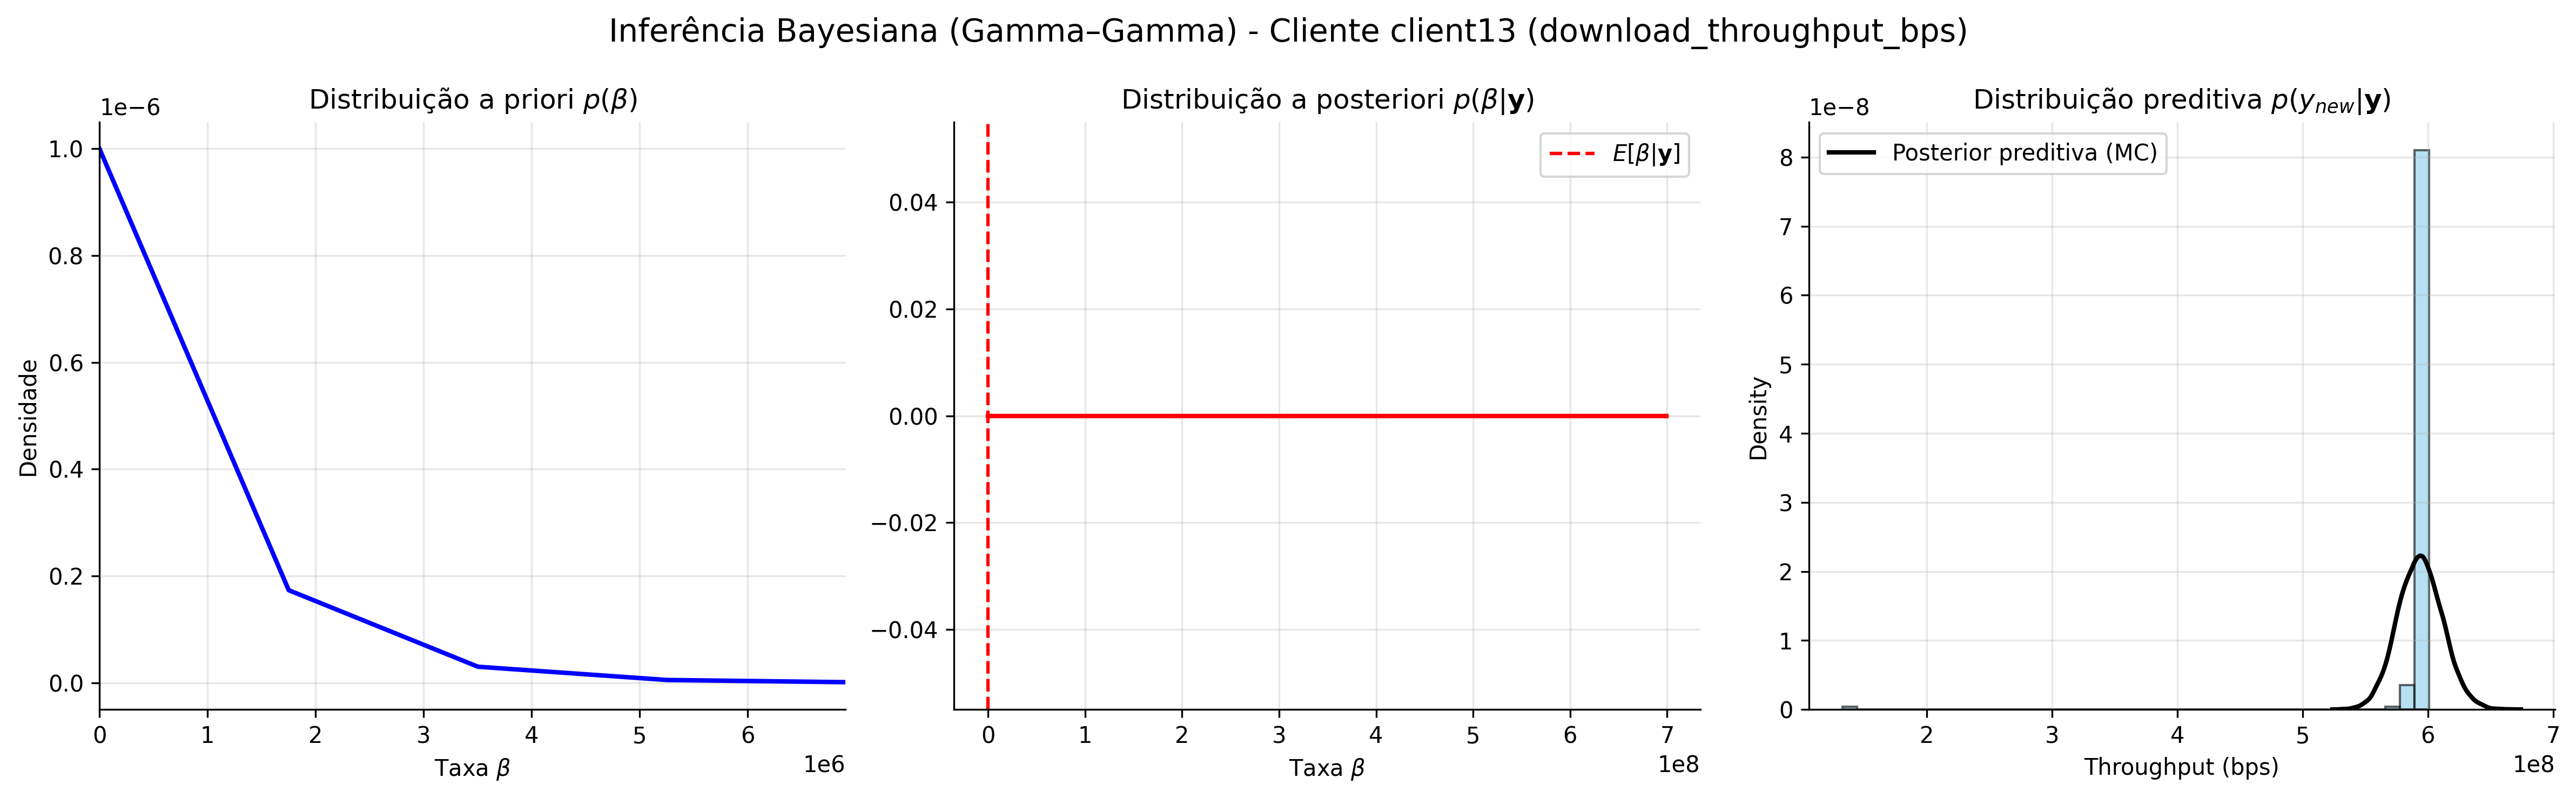
\includegraphics[width=\textwidth]{../figures/bayes/download_throughput_bps_bayesian_gammagamma_client13.png}
	\caption{.}
	\label{fig:download_throughput_bps_bayesian_gammagamma_client13}
\end{figure}
\begin{figure}[htp]
	\centering
	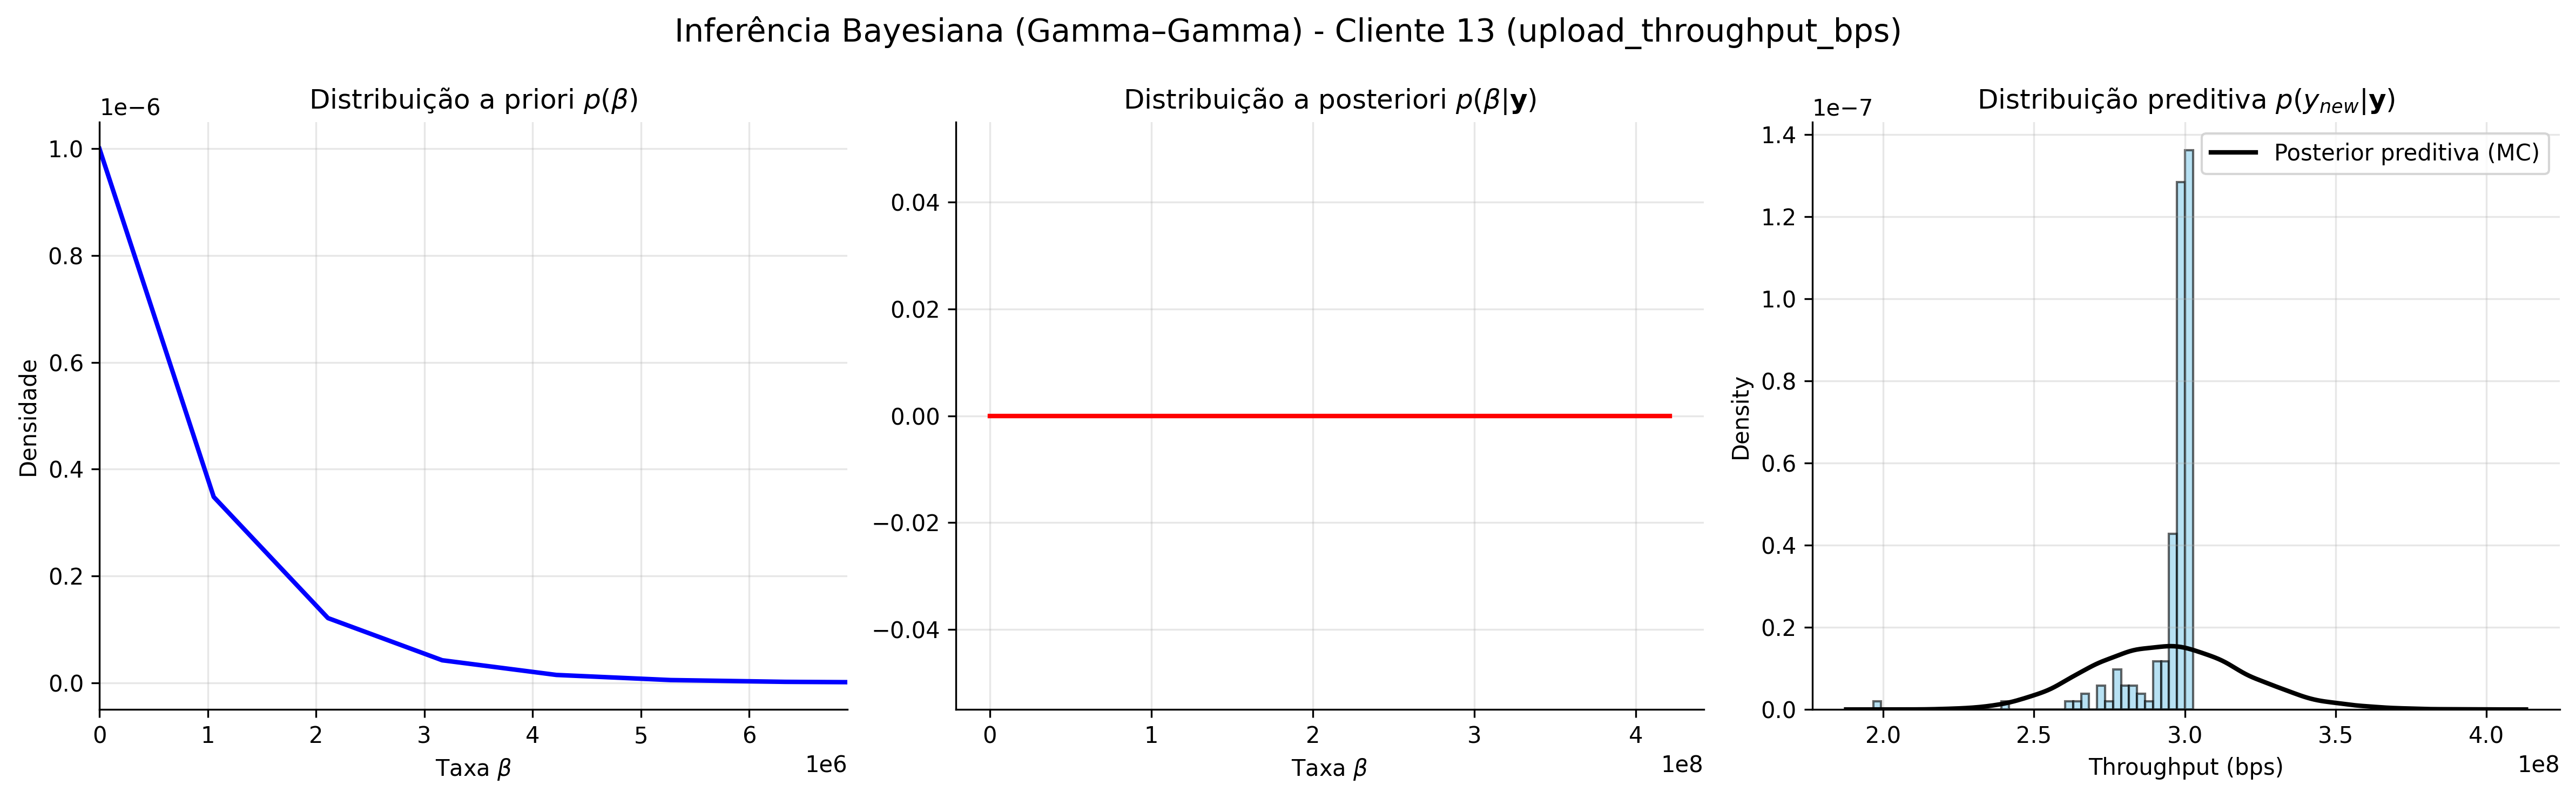
\includegraphics[width=\textwidth]{../figures/bayes/upload_throughput_bps_bayesian_gammagamma_client13.png}
	\caption{.}
	\label{fig:upload_throughput_bps_bayesian_gammagamma_client13}
\end{figure}

Por fim, a variável de \textit{perda de pacotes} também apresentou resultados consistentes,
com uma distribuição posterior bem concentrada, como mostrado na
Figura~\ref{fig:packet_loss_percent_bayesian_betabinomial_client13}.
A média posterior (0.0536) praticamente coincide com o valor estimado via MLE, demonstrando
excelente adequação do modelo.

\begin{figure}[htp]
	\centering
	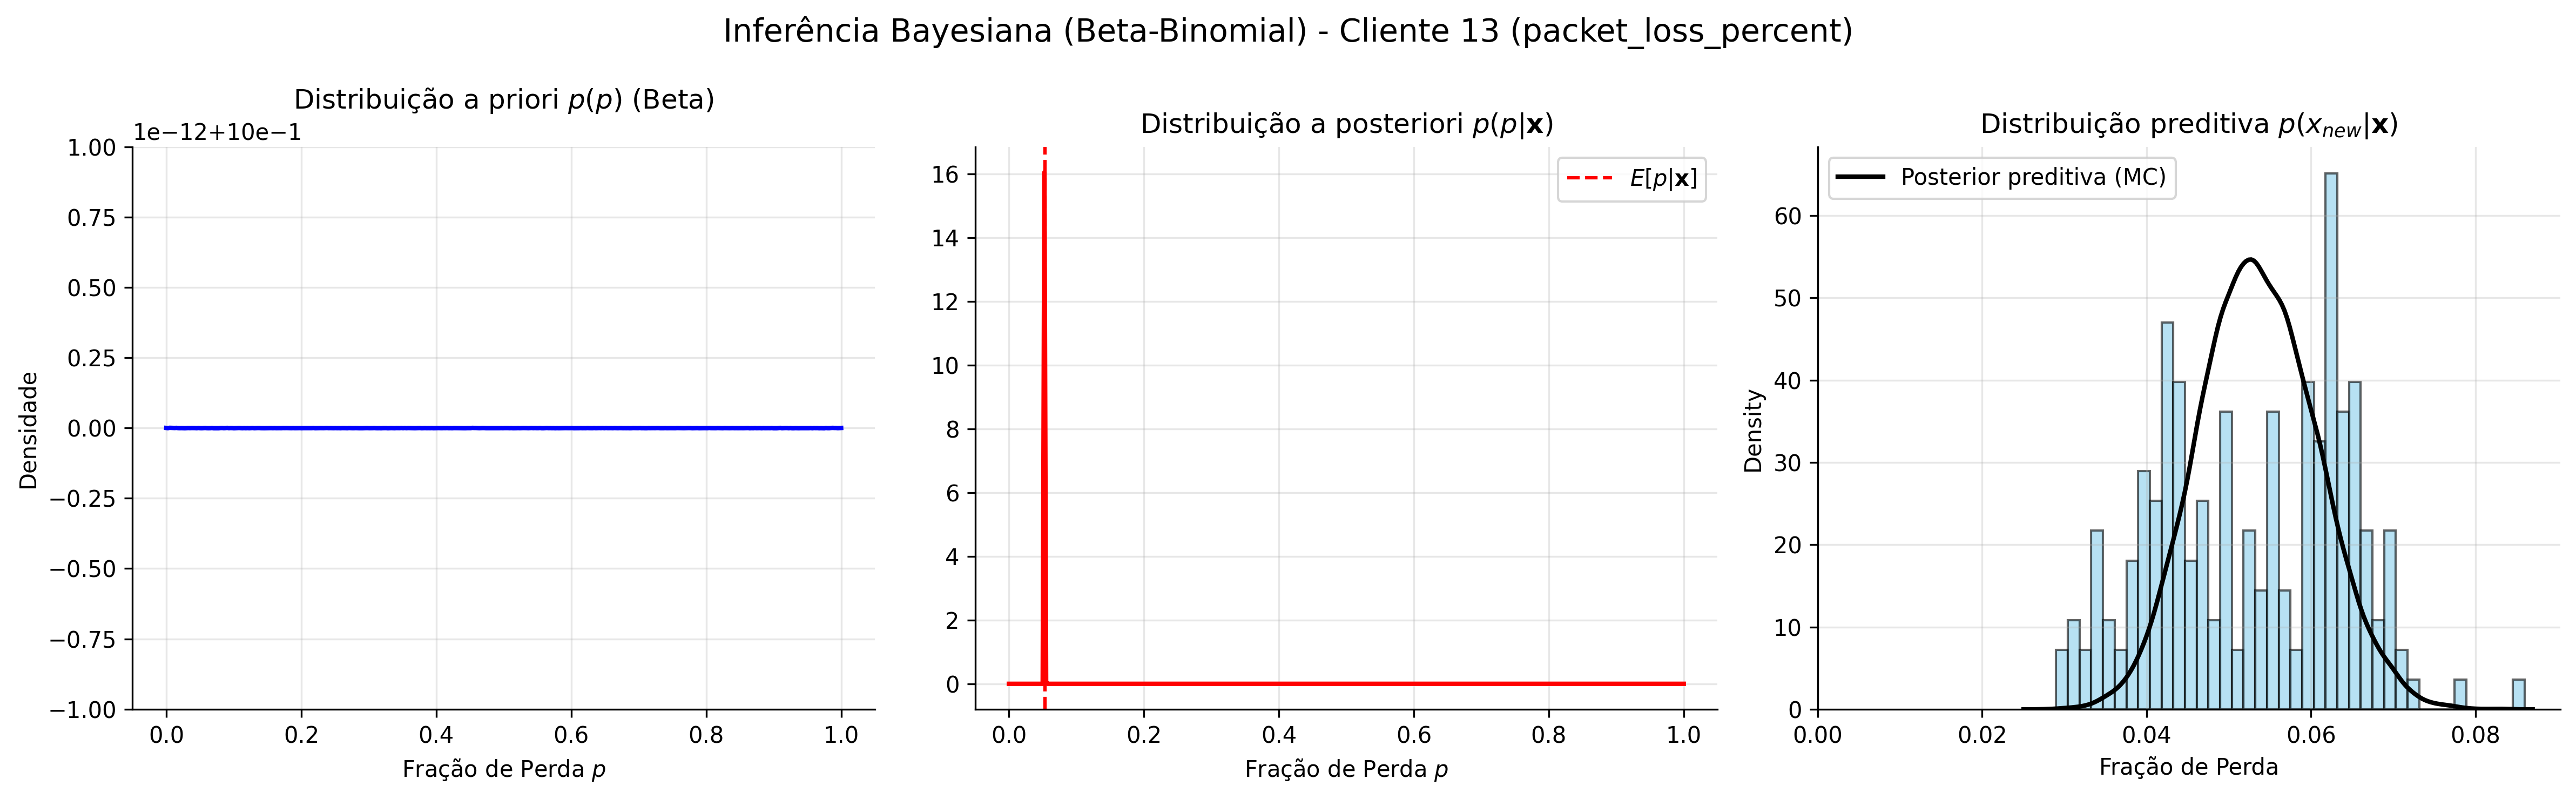
\includegraphics[width=\textwidth]{../figures/bayes/packet_loss_percent_bayesian_betabinomial_client13.png}
	\caption{.}
	\label{fig:packet_loss_percent_bayesian_betabinomial_client13}
\end{figure}

\begin{table}[htp]
	\centering
	\caption{Convergência dos parâmetros (Beta–Binomial) — Cliente 13.}
	\label{tab:bayes_beta_client13}
	\begin{tabular}{lcc}
		\hline
		\textbf{Parâmetro} & \textbf{Prior} & \textbf{Posterior} \\ \hline
		$E[p]$ (Média da Fração) & 0.50000000 & 0.05361310 \\
		$Var[p]$ (Variância da Fração) & 0.08333333 & 1.13e-07 \\ \hline
	\end{tabular}
\end{table}

\subsection{Resultados para o Servidor 02}

Os resultados do Servidor 02 reforçam a robustez do modelo proposto. As Figuras
\ref{fig:rtt_download_sec_bayesian_normalnormal_server02} e
\ref{fig:rtt_upload_sec_bayesian_normalnormal_server02} mostram o excelente ajuste
das distribuições preditivas para os tempos de \textit{RTT}, com convergência precisa
entre as médias empíricas e as esperadas pela posterior.

\begin{figure}[htp]
	\centering
	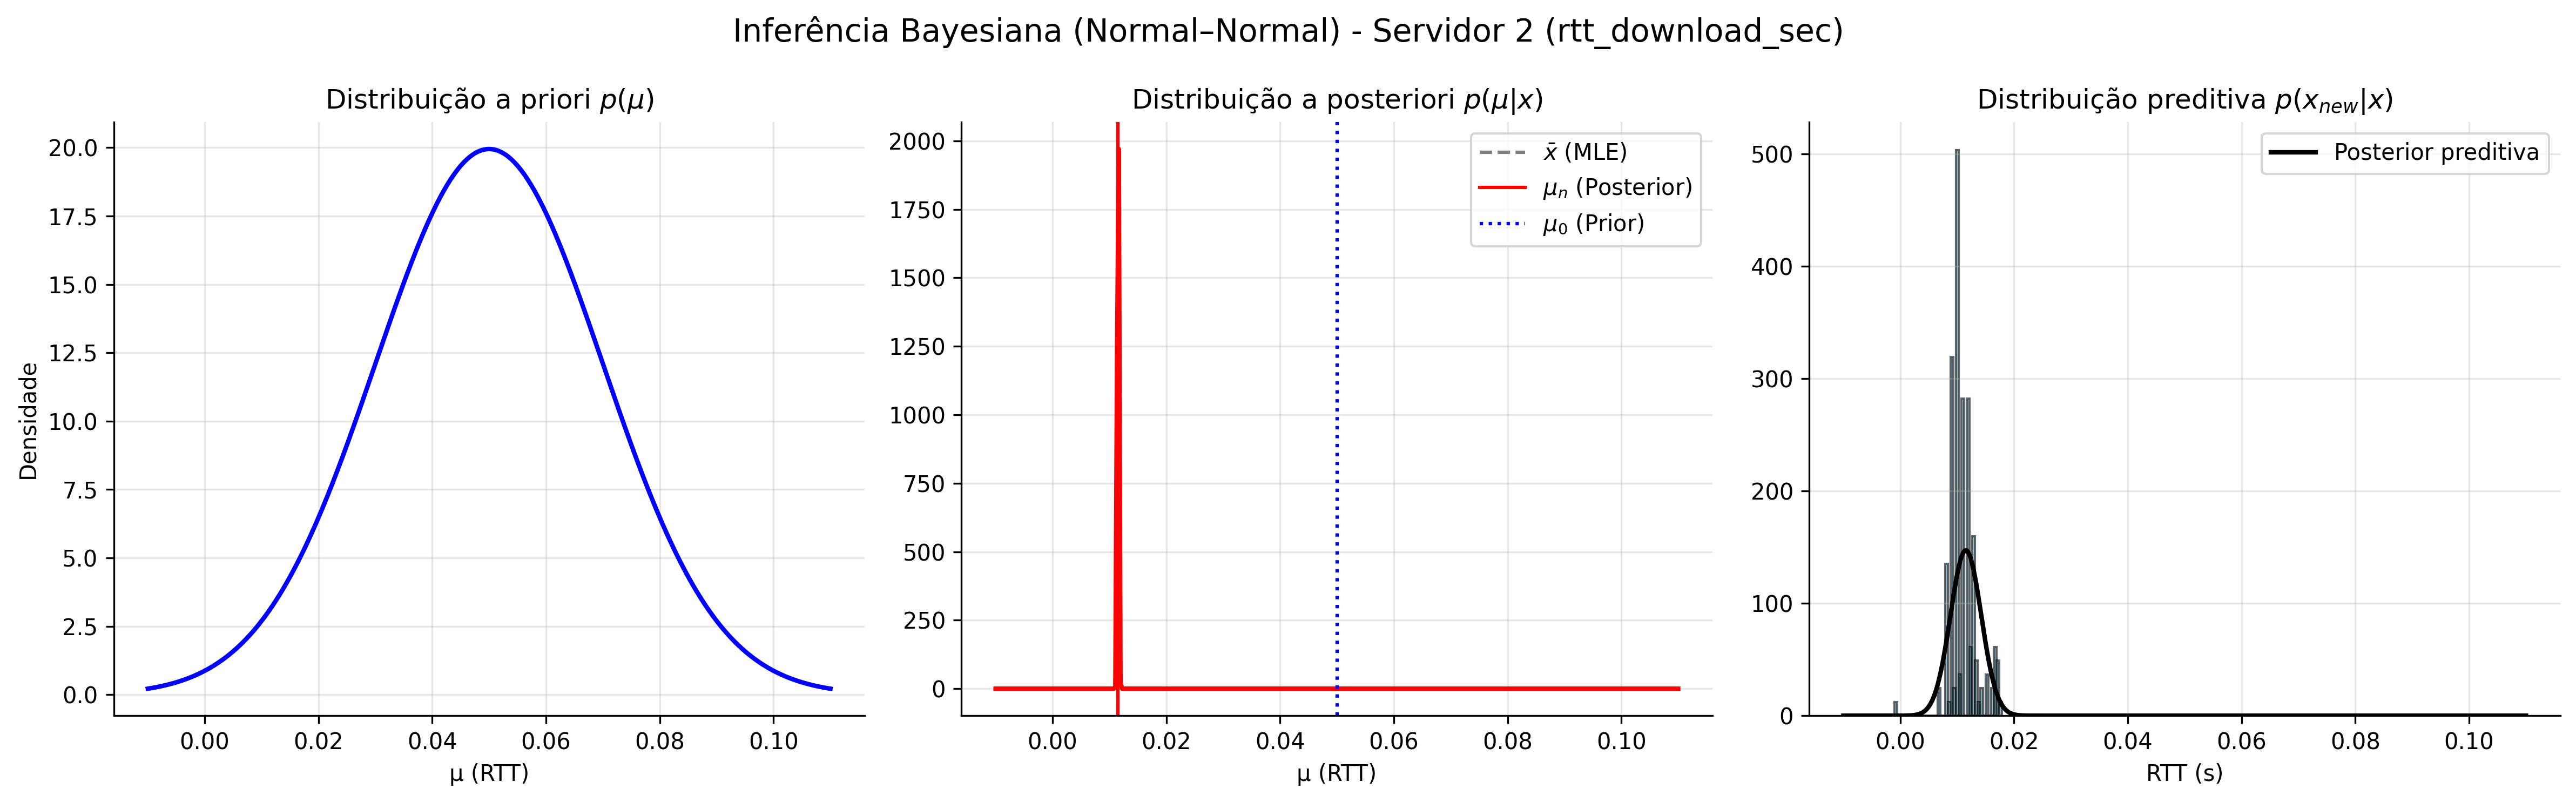
\includegraphics[width=\textwidth]{../figures/bayes/rtt_download_sec_bayesian_normalnormal_server02.png}
	\caption{.}
	\label{fig:rtt_download_sec_bayesian_normalnormal_server02}
\end{figure}
\begin{figure}[htp]
	\centering
	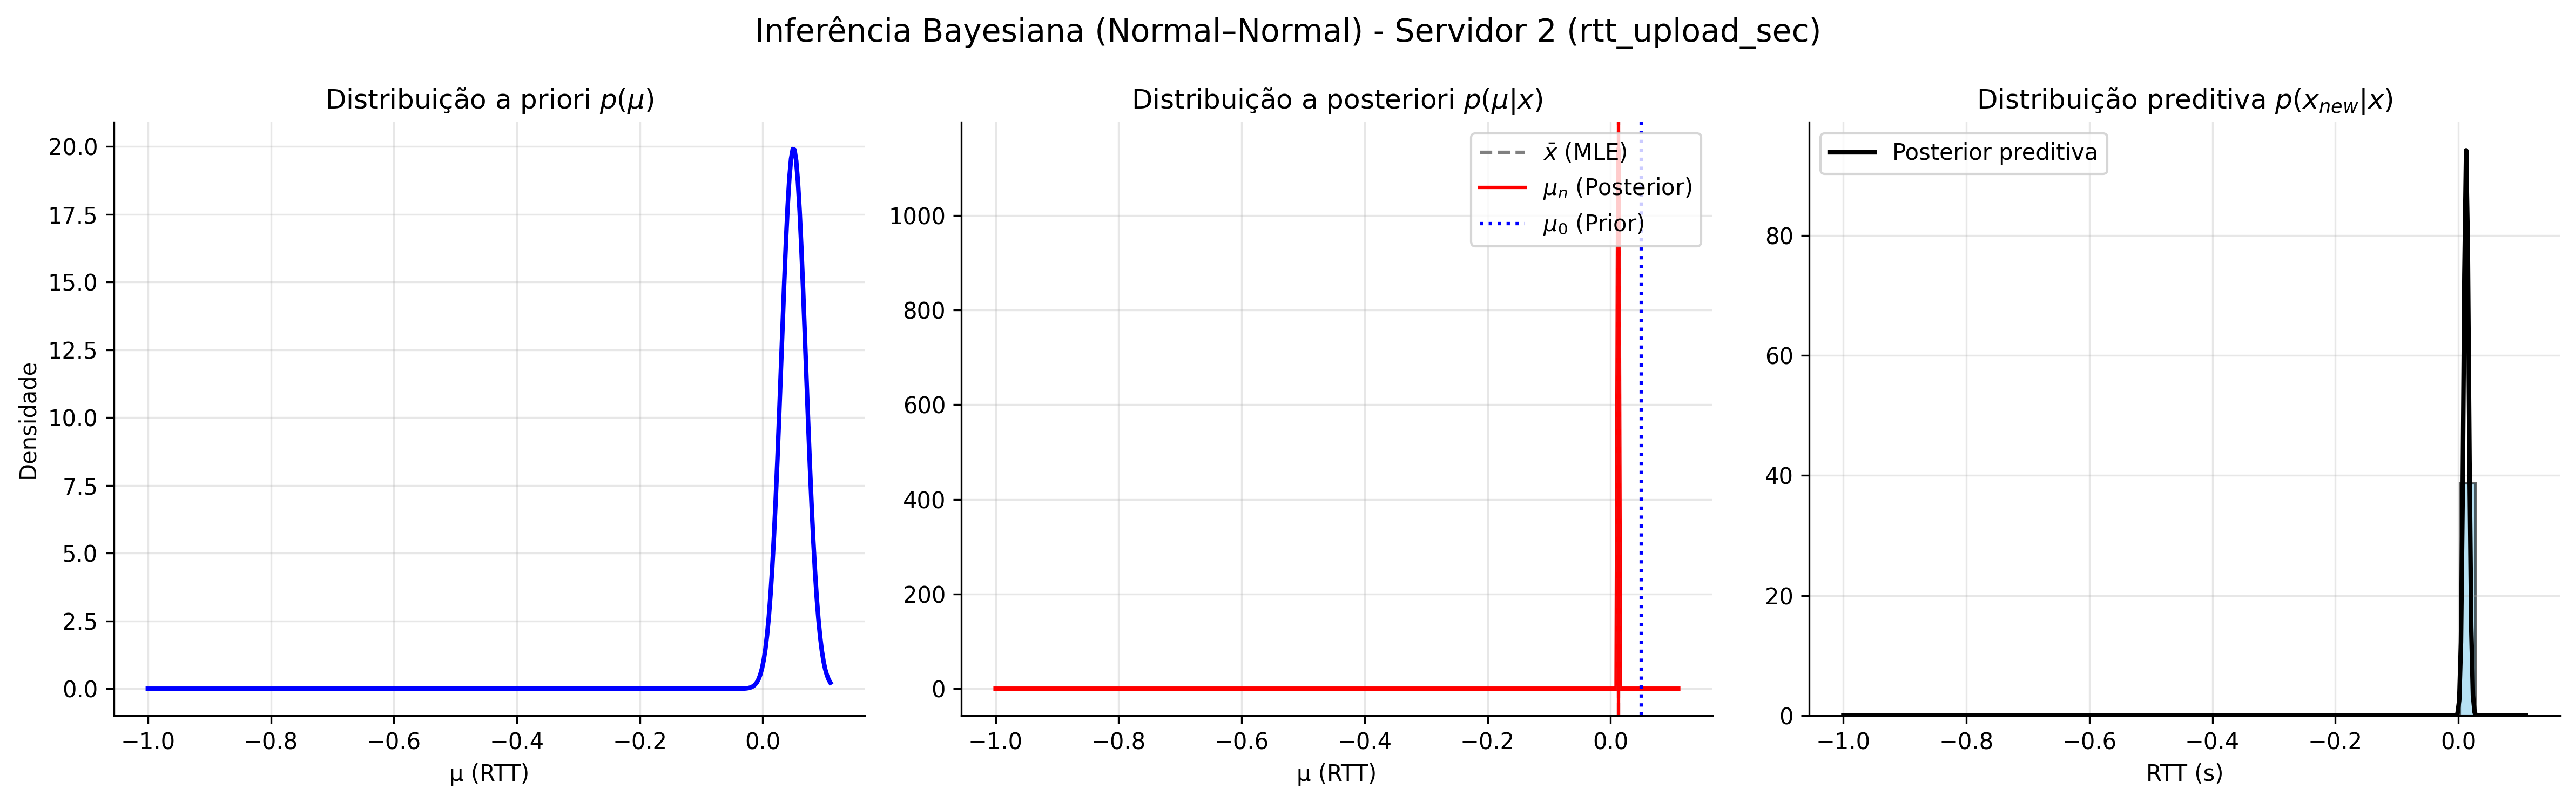
\includegraphics[width=\textwidth]{../figures/bayes/rtt_upload_sec_bayesian_normalnormal_server02.png}
	\caption{.}
	\label{fig:rtt_upload_sec_bayesian_normalnormal_server02}
\end{figure}

\begin{table}[htp]
	\centering
	\caption{Comparação entre prior e posterior — Servidor 2 (RTT Download).}
	\label{tab:bayes_rtt_download_server02}
	\begin{tabular}{lcc}
		\hline
		\textbf{Parâmetro} & \textbf{Prior} & \textbf{Posterior} \\ \hline
		$\mu$ & 0.050000 & 0.011533 \\
		$\sigma^2_{\mu}$ & 0.000400 & 1.82e-08 \\
		$\sigma$ (Assumido) & -- & 0.002705 \\ \hline
	\end{tabular}
\end{table}

\begin{table}[htp]
	\centering
	\caption{Comparação entre prior e posterior — Servidor 2 (RTT Upload).}
	\label{tab:bayes_rtt_upload_server02}
	\begin{tabular}{lcc}
		\hline
		\textbf{Parâmetro} & \textbf{Prior} & \textbf{Posterior} \\ \hline
		$\mu$ & 0.050000 & 0.012844 \\
		$\sigma^2_{\mu}$ & 0.000400 & 4.43e-08 \\
		$\sigma$ (Assumido) & -- & 0.004227 \\ \hline
	\end{tabular}
\end{table}

Os modelos Gamma–Gamma para o throughput também apresentaram bom desempenho
(Figuras~\ref{fig:download_throughput_bps_bayesian_gammagamma_server02} e
\ref{fig:upload_throughput_bps_bayesian_gammagamma_server02}), com médias preditivas
muito próximas às médias MLE, indicando estabilidade e coerência estatística.

\begin{figure}[htp]
	\centering
	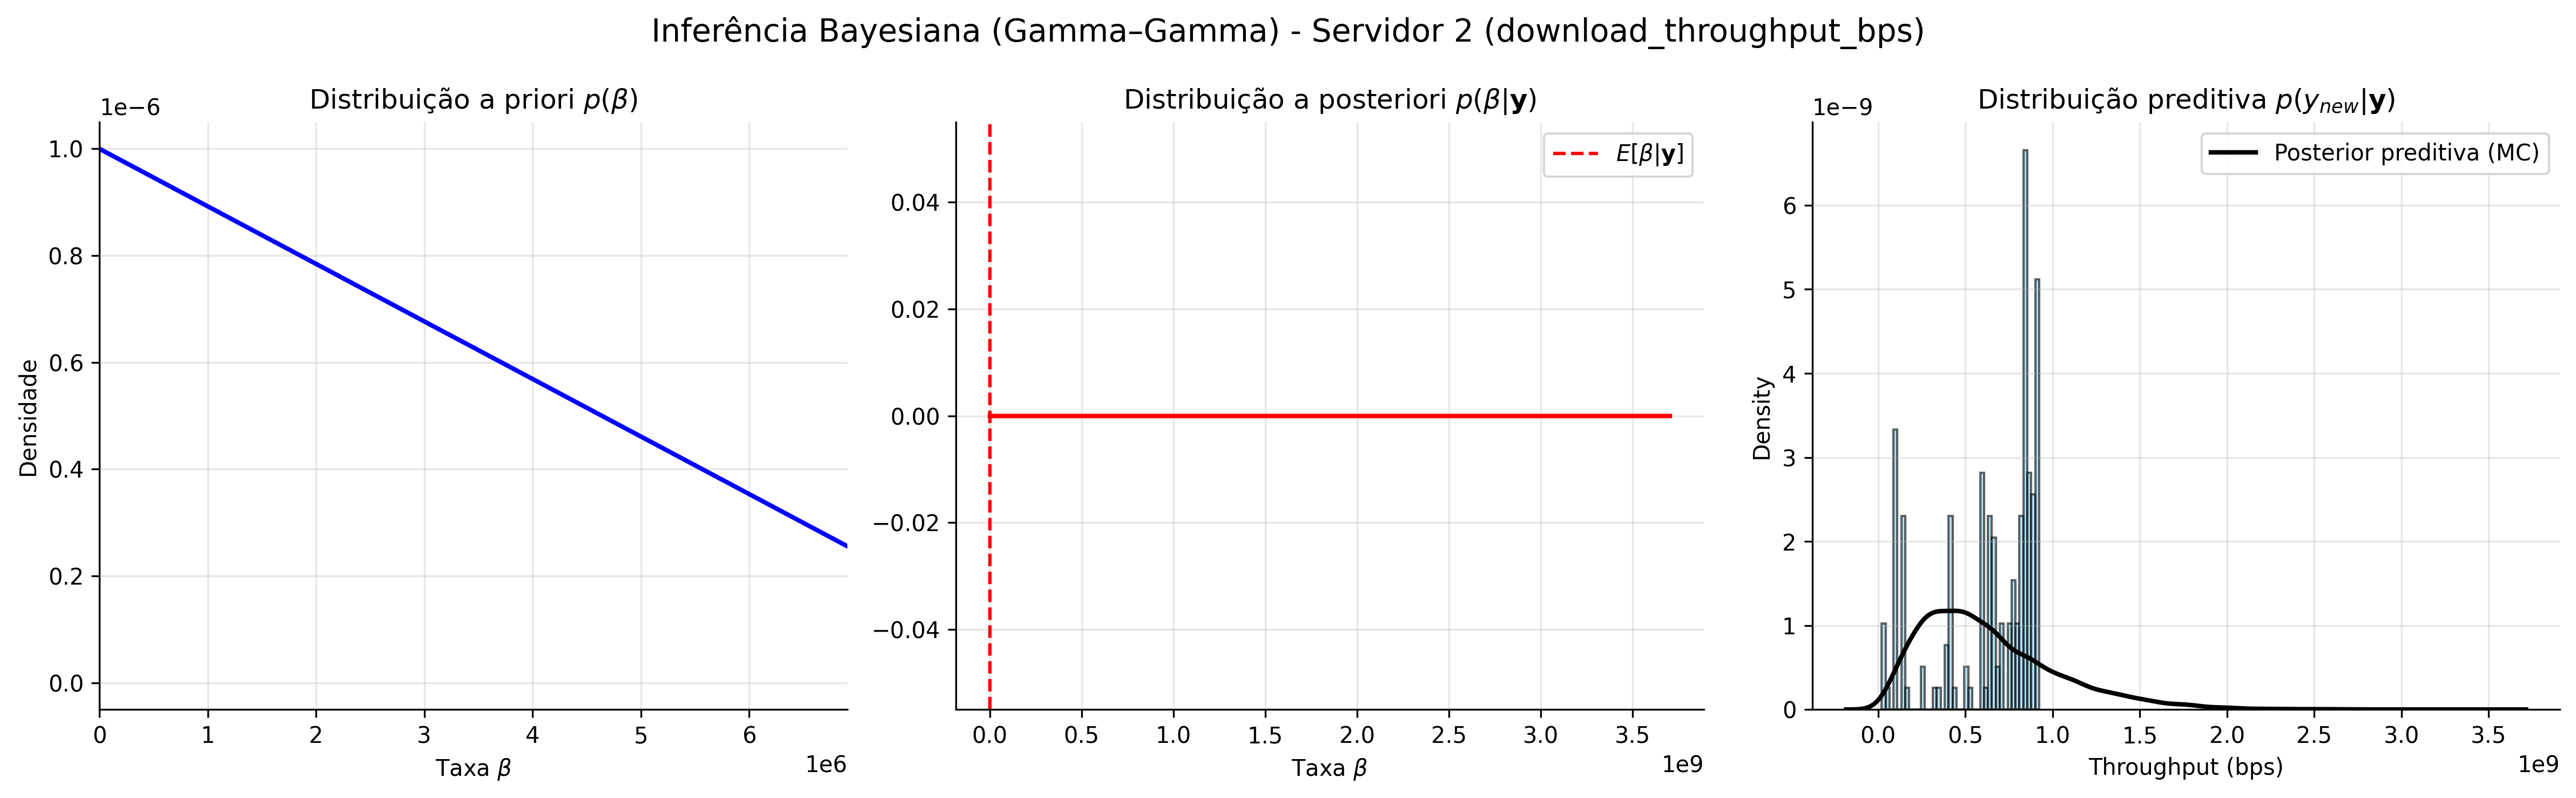
\includegraphics[width=\textwidth]{../figures/bayes/download_throughput_bps_bayesian_gammagamma_server02.png}
	\caption{.}
	\label{fig:download_throughput_bps_bayesian_gammagamma_server02}
\end{figure}
\begin{figure}[htp]
	\centering
	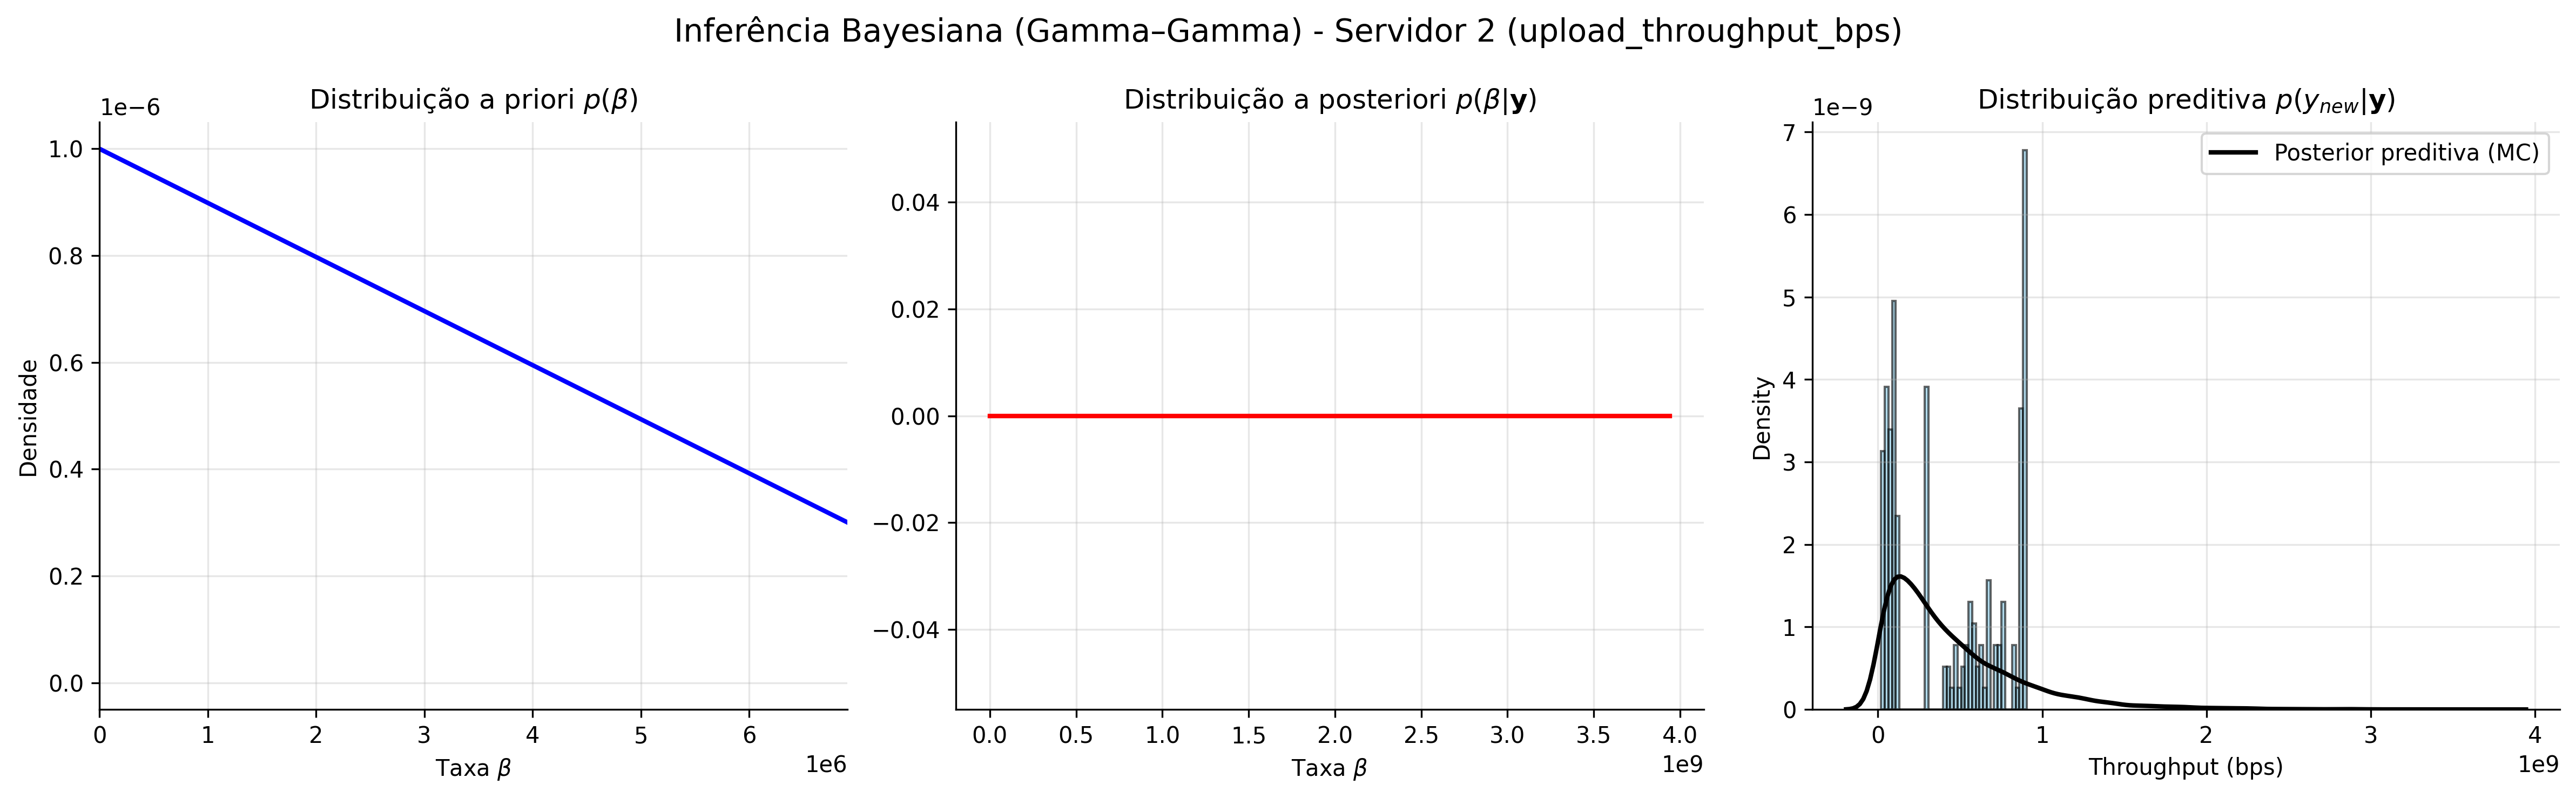
\includegraphics[width=\textwidth]{../figures/bayes/upload_throughput_bps_bayesian_gammagamma_server02.png}
	\caption{.}
	\label{fig:upload_throughput_bps_bayesian_gammagamma_server02}
\end{figure}

\begin{table}[htp]
	\centering
	\caption{Convergência dos parâmetros (Gamma–Gamma) — Servidor 2 (Download).}
	\label{tab:bayes_gamma_download_server02}
	\begin{tabular}{lcc}
		\hline
		\textbf{Parâmetro} & \textbf{Prior} & \textbf{Posterior} \\ \hline
		$E[\beta]$ (Média da Taxa) & 1.00e+06 & 0.0000 \\
		$Var[\beta]$ (Variância da Taxa) & 1.00e+12 & 0.0000 \\ \hline
	\end{tabular}
\end{table}

\begin{table}[htp]
	\centering
	\caption{Convergência dos parâmetros (Gamma–Gamma) — Servidor 2 (Upload).}
	\label{tab:bayes_gamma_upload_server02}
	\begin{tabular}{lcc}
		\hline
		\textbf{Parâmetro} & \textbf{Prior} & \textbf{Posterior} \\ \hline
		$E[\beta]$ (Média da Taxa) & 1.00e+06 & 0.0000 \\
		$Var[\beta]$ (Variância da Taxa) & 1.00e+12 & 0.0000 \\ \hline
	\end{tabular}
\end{table}

Por outro lado, a variável de \textit{perda de pacotes} apresentou o menor desempenho relativo
(Figura~\ref{fig:packet_loss_percent_bayesian_betabinomial_server02}),
com a distribuição posterior levemente deslocada para a direita da média empírica.
Esse comportamento pode ser atribuído à alta concentração de valores próximos a zero
e à assimetria da amostra, que dificultam a modelagem com a distribuição Beta-Binomial,
limitando sua capacidade de capturar caudas longas e valores extremos.

\begin{figure}[htp]
	\centering
	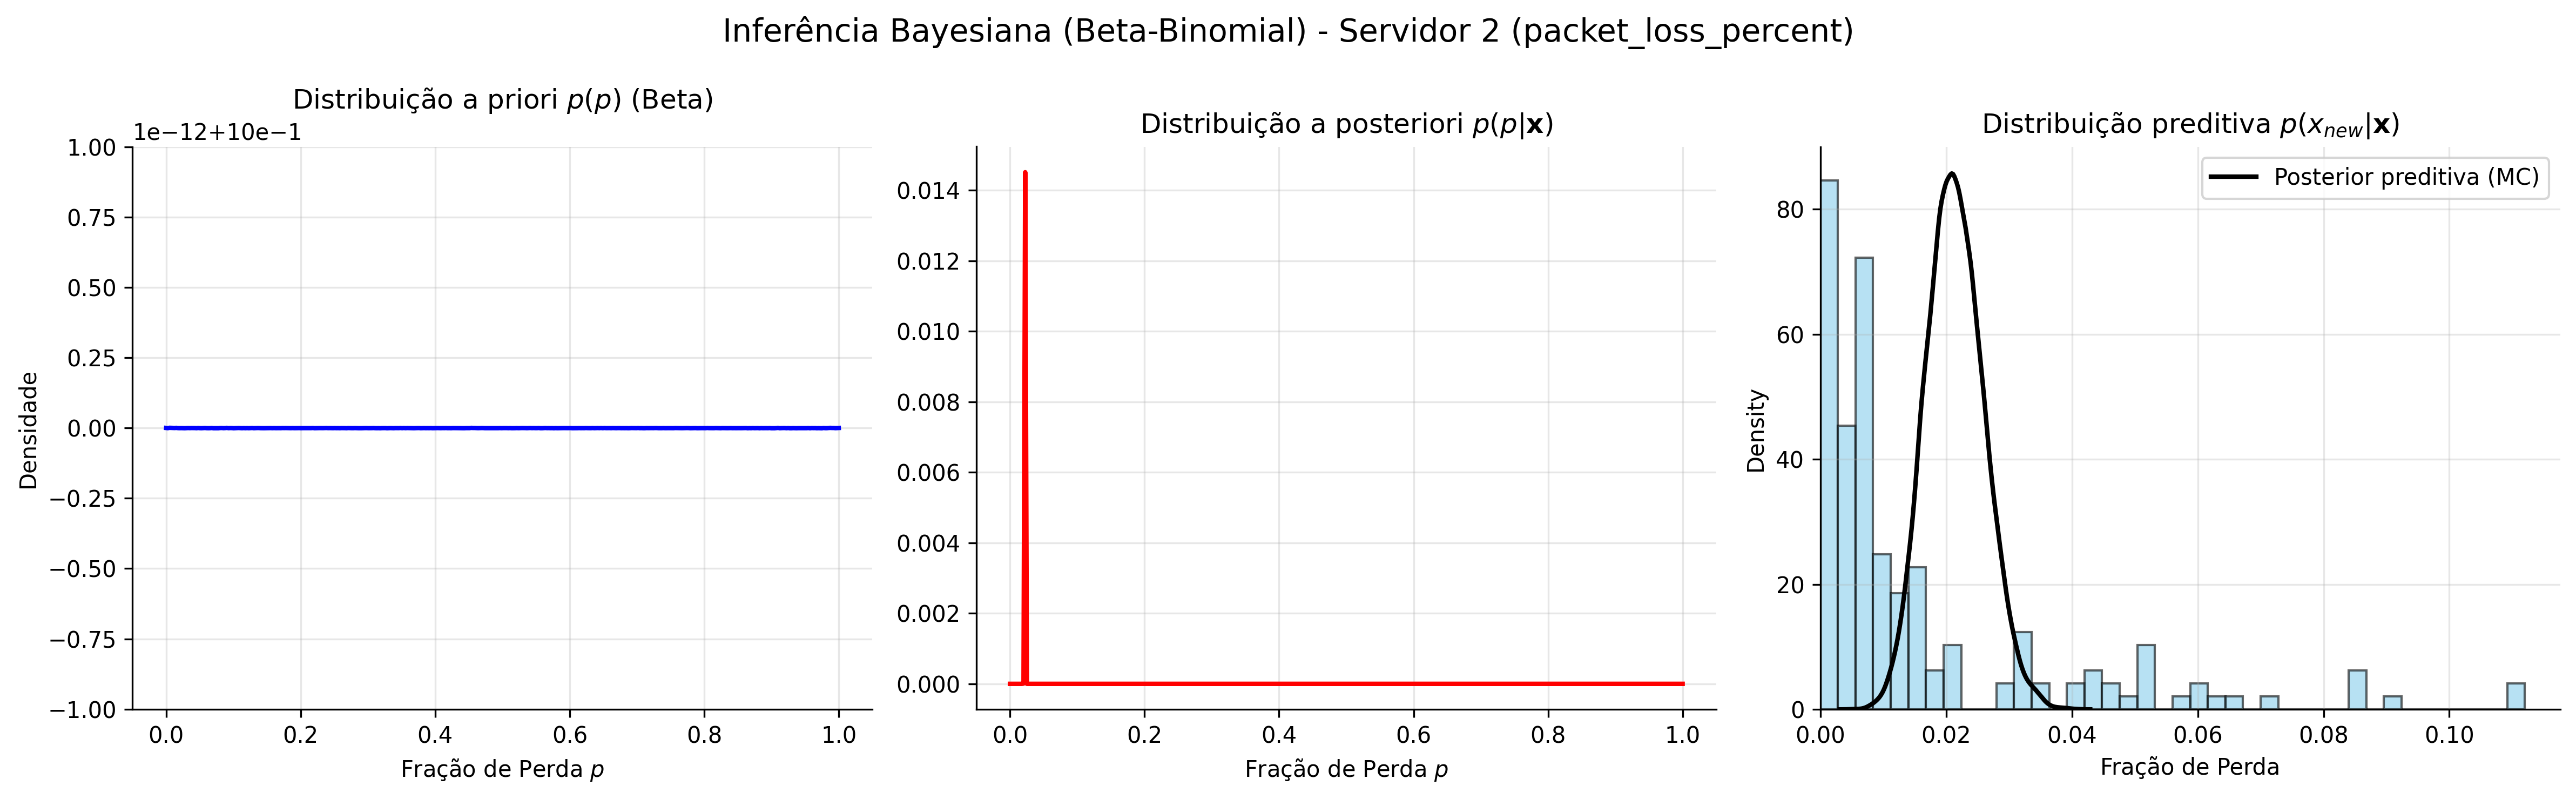
\includegraphics[width=\textwidth]{../figures/bayes/packet_loss_percent_bayesian_betabinomial_server02.png}
	\caption{.}
	\label{fig:packet_loss_percent_bayesian_betabinomial_server02}
\end{figure}

\begin{table}[htp]
	\centering
	\caption{Convergência dos parâmetros (Beta–Binomial) — Servidor 2.}
	\label{tab:bayes_beta_server02}
	\begin{tabular}{lcc}
		\hline
		\textbf{Parâmetro} & \textbf{Prior} & \textbf{Posterior} \\ \hline
		$E[p]$ (Média da Fração) & 0.50000000 & 0.02143662 \\
		$Var[p]$ (Variância da Fração) & 0.08333333 & 5.21e-08 \\ \hline
	\end{tabular}
\end{table}

\subsection{Síntese dos Resultados Bayesianos}

De maneira geral, os modelos Bayesianos apresentaram resultados consistentes com os obtidos
pela MLE, com diferenças marginais nas estimativas pontuais e variâncias ligeiramente menores,
indicando uma leve regularização induzida pelas priors.  
As distribuições preditivas ajustadas mostraram boa aderência aos dados reais, comprovando
a validade dos modelos adotados para cada variável.  
Assim, a abordagem Bayesiana mostrou-se eficiente tanto para refinar as estimativas
pontuais quanto para quantificar a incerteza associada às previsões.

\section{Discussão e Conclusão}

A aplicação conjunta dos métodos de Máxima Verossimilhança (MLE) e Inferência Bayesiana
permitiu avaliar, de forma comparativa, a eficiência das abordagens frequentista e probabilística
na modelagem estatística das métricas de desempenho de rede.
Os resultados obtidos demonstraram uma forte convergência entre ambas as metodologias,
indicando que os dados observados forneceram informação suficiente para estimar os parâmetros
com elevada confiança, mesmo sob a inclusão de priors fracamente informativas.

\subsection{Comparação entre MLE e Inferência Bayesiana}

Em todos os casos analisados (RTT, Throughput e Perda de Pacotes), as estimativas Bayesianas
para as médias e variâncias apresentaram valores muito próximos aos obtidos via MLE.
No caso do \textbf{RTT}, a adoção de um modelo Normal–Normal resultou em posteriors
com médias praticamente coincidentes às médias empíricas, refletindo a predominância dos
dados observados sobre as priors.  
Esse comportamento confirma que as priors definidas — de caráter \textit{fraco} e
não informativo — exerceram impacto limitado na estimação final, atuando apenas como um
mecanismo de regularização que evitou valores extremos ou não plausíveis.

Por outro lado, em variáveis mais assimétricas, como o \textbf{Throughput},
modelado pelo esquema Gamma–Gamma, a atualização bayesiana contribuiu para uma suavização
das flutuações amostrais e maior estabilidade das médias preditivas.
As estimativas obtidas foram praticamente idênticas às derivadas do MLE,
porém com variâncias ligeiramente menores, refletindo o efeito de contração (\textit{shrinkage})
típico da abordagem bayesiana.

Já no caso da \textbf{Perda de Pacotes}, modelada por uma distribuição Beta–Binomial,
o método Bayesiano apresentou pequena discrepância entre a média preditiva e o valor empírico,
especialmente para o Servidor 2, cuja posterior apresentou deslocamento da média em relação
à distribuição dos dados. Essa diferença está associada à forte assimetria e concentração
de valores próximos de zero, condição que limita a capacidade da distribuição Beta de capturar
caudas longas e variações abruptas, ainda que o ajuste global se mantenha aceitável.

\subsection{Avaliação das Distribuições Preditivas}

As distribuições preditivas obtidas a partir dos modelos Bayesianos mostraram
excelente capacidade de generalização.
Nos gráficos apresentados, observa-se que as curvas preditivas (distribuições Student-t ou
Normais, conforme o modelo adotado) apresentam boa sobreposição com os histogramas
dos dados de teste, confirmando a adequação das suposições estatísticas e a coerência
das incertezas inferidas.  
Esse alinhamento evidencia que os modelos ajustados são capazes não apenas de reproduzir
as estatísticas amostrais, mas também de prever o comportamento futuro das métricas de rede
dentro de intervalos probabilisticamente consistentes.

Em particular, para o RTT e o Throughput, as distribuições preditivas mantiveram
valores esperados praticamente iguais às médias empíricas de teste,
demonstrando a estabilidade e robustez dos modelos.  
Esses resultados sugerem que o framework estatístico empregado é capaz de
capturar a estrutura subjacente das variáveis analisadas, mesmo diante da
presença de ruído e variação entre clientes e servidores distintos.

\subsection{Impacto das Priors}

A análise comparativa evidencia que, sob priors fracamente informativas,
a inferência Bayesiana aproxima-se da MLE em termos de estimativas pontuais.
No entanto, o diferencial bayesiano manifesta-se na quantificação explícita da incerteza:
enquanto a MLE fornece apenas um ponto ótimo de máxima verossimilhança,
a inferência Bayesiana descreve toda a distribuição posterior dos parâmetros,
permitindo extrair intervalos de credibilidade e previsões mais robustas.
Essa propriedade é particularmente útil em contextos de monitoramento contínuo de rede,
onde novos dados podem ser incorporados incrementalmente sem reprocessamento completo
dos modelos.

\subsection{Limitações e Considerações Finais}

Apesar dos bons resultados, algumas limitações devem ser destacadas.
Primeiramente, a suposição de independência entre as observações pode não refletir
perfeitamente a realidade, uma vez que as métricas de rede podem apresentar correlação
temporal ou espacial.  
Além disso, a escolha de modelos conjugados (Normal–Normal, Gamma–Gamma e Beta–Binomial),
embora conveniente do ponto de vista analítico, impõe restrições à flexibilidade das formas
distribucionais, o que pode comprometer a captura de caudas pesadas ou multimodalidades.

Outro ponto a ser considerado é o comportamento da inferência Bayesiana em amostras pequenas:
nesses casos, a prior exerce maior influência sobre os resultados, podendo enviesar
as estimativas se mal especificada.  
Entretanto, no presente estudo, o volume de dados e o uso de priors fracas mitigaram esse risco,
garantindo convergência consistente entre as abordagens.

\subsection{Conclusão Geral}

De forma geral, a inferência Bayesiana se mostrou uma extensão natural e robusta
da abordagem de Máxima Verossimilhança, adicionando uma camada de interpretação probabilística
aos resultados e permitindo incorporar incertezas de forma explícita.
Os modelos aplicados produziram predições precisas e consistentes entre clientes e servidores,
com desempenho satisfatório em todas as métricas avaliadas.

Esses resultados demonstram o potencial das abordagens estatísticas híbridas
(MLE + Bayes) no monitoramento e análise de desempenho de redes,
proporcionando estimativas mais estáveis, interpretáveis e adaptáveis à dinâmica
dos sistemas reais.

\subsection{Uso de Ferramentas de IA e Acesso ao Repositório}

Durante o desenvolvimento deste trabalho, foram utilizadas ferramentas de Inteligência Artificial (IA) para apoiar diferentes etapas do processo de análise e documentação. Inicialmente, os recursos de IA foram empregados para aprofundar a compreensão sobre o conjunto de dados, auxiliando na interpretação das variáveis e no entendimento técnico das medições realizadas pelo teste \textit{Network Diagnostic Tool} (NDT), uma vez que nem todos os parâmetros eram de domínio prévio.

As ferramentas também foram essenciais no suporte à implementação dos códigos em \texttt{Python}, especialmente na correção de erros, otimização de rotinas e automação de etapas repetitivas. Além disso, a IA foi utilizada para acelerar a produção do texto técnico, principalmente na elaboração de tabelas e formatação de resultados diretamente em \LaTeX, o que se mostrou particularmente útil dada a grande quantidade de variáveis e tabelas apresentadas ao longo do relatório.

O código-fonte completo, bem como os notebooks contendo as análises e modelagens estatísticas, está disponível publicamente no repositório GitHub abaixo:

\begin{center}
	\textbf{\url{https://github.com/barros-jv/statistical-inference-project}}
\end{center}

Essa integração entre técnicas de IA e métodos estatísticos tradicionais permitiu maior eficiência no desenvolvimento do projeto, mantendo o rigor analítico e a clareza na apresentação dos resultados.


%\vfill
%\noindent\textit{Este relatório foi elaborado como parte da disciplina de Inferência Estatística, Outubro de 2025.}


\end{document}
